\part{The /um/ <\armenian{ում}> branch}

The /um/ <\armenian{ում}> branch has 7 dialects:

\begin{enumerate}
	\item Dialect of Yerevan (\S\ref{chapter:Yerevan})
	\item Dialect of Tbilisi (\S\ref{chapter:Tbilisi})
	\item Dialect of Karabakh (\S\ref{chapter:Karabakh})
	\item Dialect of Shamakhi (\S\ref{chapter:Shamakhi})
	\item Dialect of Astrakhan (\S\ref{chapter:Astrakhan})
	\item Dialect of Julfa (\S\ref{chapter:Julfa})
	\item Dialect of Agulis (\S\ref{chapter:Agulis})
	
\end{enumerate}




\chapter{Yerevan}\label{chapter:Yerevan}



\begin{adjarianpage}\label{page:37}\end{adjarianpage}% should be 37

\section{Background}
The Yerevan dialect is spoken in the city of Yerevan and in the surrounding provinces, especially in the provinces of Yerevan, Etchmiadzin, and New Bayazet. It spreads from the south side to Tabriz, the capital of Atropatene (Iranian Azerbaijan), from the west Kaghzvan, from the southwest side it enters Ottoman Turkey and it reaches until Bayazit, from the northern and southern sides it gets mixed with the Karin and Karabakh dialects, which demarcate its two borders. On its north sides, the Yerevan dialect forms two islets; one of them is in the province of Borchaly (Shulaver, Shamshadin, Lori, and the surrounding areas), and the second is in Avlabari district of Tbilisi, which is a migrant settlement of Yerevan. 


Besides the main dialect, the Yerevan dialect has three subdialects, which are the following:

\begin{itemize}
	\item Bayazit subdialect: This in Ottoman Armenia. Its one settlement is the city of New Bayazet, the shores of Lake Sevan, with 10 surrounding Armenian-populated villages. These are Ordaklu, Noraduz, Gyshlag, Bashkend, Kösemehmet, Kulali, Kyarimkend, Dalikardash, Kyuzadzhik, and Bashkend. This entire region speaks the same dialect, as in Bayazit. 
	\item Astabad subdialect: This is spoken near Old Julfa in the village of Astabad and its surrounding area.
	\item Tabriz subdialect: In Atropatene  (Iranian Azerbaijan), the Armenian settlement in Tabriz has two districts: Ghala and Lilava. The people of Lilava are much larger and they have recently migrated from Karabakh; they speak the Karabakh subdialect. As for the people of Ghala, they form less than half the Armenian population of Tabriz, and they are considered natives, and they speak the Tabriz dialect.
\end{itemize}



\begin{adjarianpage}\label{page:38}\end{adjarianpage}% should be 38

The Yerevan dialect is very pure and it is very close to the literary language. And if we consider only the /um/ <\armenian{ում}> dialects, then it is the purest. And thus, it is because of its pureness and its extensive size that it serves as a base for the formation of the Russian-Armenian literary language. 

\section{Phonology}

\subsection{Segment inventory}
The phonetic system of the Yerevan dialect has the following sounds in Tables \ref{tab:Yerevan:vowels} and \ref{tab:Yerevan:Consonant}. 



\begin{table}[H]
	\centering
	\caption{Vowels of the Yerevan dialect}
	\label{tab:Yerevan:vowels}
	\begin{tabular}{|lll|}
		\hline /i/ <\armenian{ի}> & &/u/ <\armenian{ու}> \\
		/e/ <\armenian{է}> & /ə/ <\armenian{ը}> & /o/ <\armenian{օ}> \\
		& & /ɑ/ <\armenian{ա}> 
		\\
		\hline 
		% Orthography & \armenian{ա} & \armenian{է} & \armenian{ը}& \armenian{ի}& \armenian{օ}& \armenian{ու} \\
		% IPA transcription & ɑ & e & ə & i & o & u 
		% \\ \hline
	\end{tabular}
\end{table}

\begin{table}[H]
	\centering
	\caption{Consonants of the Yerevan dialect}
	\label{tab:Yerevan:Consonant}
	\resizebox{\textwidth}{!}{%
	\begin{tabular}{|l|lll|llll|lll|}
		\hline 
		& \multicolumn{3}{l|}{Labial}& \multicolumn{4}{l|}{Coronal}& \multicolumn{3}{l|}{Dorsal/back}\\
		Stops& /b/ & /p/ & /pʰ/ & /d/ & /t/ & /tʰ/& & /ɡ/ & /k/ & /kʰ/ 
		\\
		& <\armenian{բ}> &<\armenian{պ}>& <\armenian{փ}> &<\armenian{դ}>& <\armenian{տ}> &<\armenian{թ}>&& <\armenian{գ}>& <\armenian{կ}>& <\armenian{ք}>\\
		\hline 
		Affricates & && & /d͡z/ & /t͡s/ & /t͡sʰ/ & && & \\
		& && &<\armenian{ձ}>& <\armenian{ծ}>& <\armenian{ց}> & & & & \\
		& && & /d͡ʒ/ & /t͡ʃ/ & / t͡ʃʰ/ && & & \\
		& & & &<\armenian{ջ}>& <\armenian{ճ}>& <\armenian{չ}> & & && \\
		\hline 
		Fricatives& /f/ & /v/ & &/s/& /z/& /ʃ/& /ʒ/& /χ/ & /ʁ/ & /h/ \\
		& <\armenian{ֆ}> & <\armenian{վ}>& & <\armenian{ս}>& <\armenian{զ}>& <\armenian{շ}>& <\armenian{ժ}>& <\armenian{խ}> & <\armenian{ղ}> & <\armenian{հ}>
		\\ \hline 
		Sonorants & /m/ & /n/& & /ɾ/ & /r/& /l/ & /j/ && & \\
		& <\armenian{մ}> & <\armenian{ն}> && <\armenian{ր}>& <\armenian{ռ}>& <\armenian{լ}>& <\armenian{յ}> && & 
		\\ \hline 
	\end{tabular}
}\end{table}

Like other Armenian dialects, the Yerevan dialect does not have diphthongs. The diphthongs of Old Armenian have become either simple vowels (Table \ref{tab:Yerevan:DiphthongLoss}a) or have turned into a consonant-vowel sequence (Table \ref{tab:Yerevan:DiphthongLoss}b). 


\begin{table}[H]
	\centering
	\caption{Loss of Classical diphthongs in Yerevan Armenian}
	\label{tab:Yerevan:DiphthongLoss}
	\begin{tabular}{|l| ll|ll| ll|}
		\hline & \multicolumn{2}{l|}{Classical Armenian} &\multicolumn{2}{l|}{> Yerevan} & \multicolumn{2}{l|}{cf. SEA} \\ 
		a. `father' & hɑi̯ɾ & \armenian{հայր}& heɾ & \armenian{հէր} & hɑjɾ & \armenian{հայր} \\ 
		b. `God' & ɑstu̯ɑt͡s & \armenian{Աստուած} & ɑstvɑd͡z & \armenian{Աստվաձ} & ɑstvɑt͡s & \armenian{Աստված}
		\\ \hline 
	\end{tabular}
\end{table}

From this list, it appears that the Yerevan dialect has almost completely preserved the rich phonetic system of Old Armenian. Among the vowel, the Classical vowels /e-ē/ <\armenian{ե-է}> and /o-ɑu̯/ <\armenian{ո-օ}> have merged with each other; in the modern dialect, they are both pronounced as /e/ <\armenian{է}> and /o/ <\armenian{օ}>. The sounds /œ/ <\armenian{էօ}> and /ʏ/ <\armenian{իւ}> that are found in other dialects, do not exist here. Among the consonants, the only sound that was lost is Classical /w/ <\armenian{ւ}>; but it has gained the sound /f/ <\armenian{ֆ}>, about which see more below.

\subsection{Sound changes}





Among the sound changes that happened in the Yerevan dialect, the following are noticeable. 


\subsubsection{Monophthong vowels}
\paragraph{Classical Armenian /e/ <\armenian{ե}>}

The Classical Armenian /e/ <\armenian{ե}> has become /je/ <\armenian{յէ}> word-initially in monosyllables. But at the beginning of polysyllabic words, it has become /e/ <\armenian{է}> among all words. Various other dialects have /i̯e/ <\armenian{ե}> and the literary language has word-initial /je/ in polysyllabic words; but these don't happen here. Examples in Table \ref{tab:Yerevan:SoundChange:Vowel:E}). 

\begin{table}[H]
	\centering
	\caption{Sound changes from CA /e/ <\armenian{ե}> in the Yerevan dialect}
	\label{tab:Yerevan:SoundChange:Vowel:E}
	\resizebox{\textwidth}{!}{%
	\begin{tabular}{|l|ll|ll|ll|}
		\hline & \multicolumn{2}{l|}{Classical Armenian}& \multicolumn{2}{l|}{> Yerevan }& \multicolumn{2}{l|}{cf. SEA }
		\\
		`I'& es & \armenian{ես} & jes & \armenian{յէս} & jes & \armenian{ես} \\
		`he has come' & eke̯ɑl ē & \armenian{եկեալ է} & ekel ɑ & \armenian{էկէլ ա} & jekel e & \armenian{եկել է} \\
		`to go' & eɾtʰɑl & \armenian{երթալ} & etʰɑl & \armenian{էթալ} & jeɾtʰɑl & \armenian{երթալ} \\
		`to cook' & epʰel & \armenian{եփել} & epʰel & \armenian{էփէլ} & jepʰel & \armenian{եփել} \\
		`dream' & eɾɑz & \armenian{երազ} & eɾɑz & \armenian{էրազ} & jeɾɑz & \armenian{երազ} \\
		`big' &met͡s & \armenian{մեծ} & met͡s& \armenian{մէծ} &met͡s & \armenian{մեծ} \\
		`grave' & ɡeɾezmɑn & \armenian{գերեզման} & ɡeɾezmɑn & \armenian{գէրէզման} & ɡeɾezmɑn & \armenian{գերեզման}
		\\ \hline
	\end{tabular}
}
\end{table}

\paragraph{Classical Armenian /o/ <\armenian{ո}>}
The Classical Armenian /o/ <\armenian{ո}>, unlike the former and like the literary language, has becomes /vo/ <\armenian{վօ}> word-initially in both monosyllabic and polysyllabic words; while it comes /o/ <\armenian{օ}> word-medially. Examples in Table \ref{tab:Yerevan:SoundChange:Vowel:O}. 



%\translatorHD{Note that oftentimes, Adjarian would provide a reflex that is actually SEA instead of CA. For example for `lentil', Adjarian gave the source word <\armenian{ոսպ}>. But the actual Classical form is <\armenian{ոսպն}>. The form <\armenian{ոսպ}> is modern. Such discrepancies are quite common in Adjarian's manuscript. {tab:Yerevan:SoundChange:Vowel:O} }

\begin{table}[H]
	\centering
	\caption{Sound changes from CA /o/ <\armenian{ո}> in the Yerevan dialect}
	\label{tab:Yerevan:SoundChange:Vowel:O}
	\resizebox{\textwidth}{!}{%
	\begin{tabular}{|l|ll|ll|ll|}
		\hline & \multicolumn{2}{l|}{Classical Armenian}& \multicolumn{2}{l|}{> Yerevan }& \multicolumn{2}{l|}{cf. SEA }
		\\
		`lentil' & ospən & \armenian{ոսպն} & vosp & \armenian{վօսպ} & vosp & \armenian{ոսպ} \\
		`gold' & oski & \armenian{ոսկի} & voski & \armenian{վօսկի} & voski& \armenian{ոսկի} \\
		`foot' & ot-(ə?)kʰ (-{\pl}) & \armenian{ոտք} & votkʰ & \armenian{վօտք} & votkʰ & \armenian{ոտք} \\
		`to massacre' & kotoɾel & \armenian{կոտորել} & kotoɾel & \armenian{կօտօրէլ} & kotoɾel & \armenian{կոտորել} \\
		`to forget' & morɑnɑl & \armenian{մոռանալ} & morɑnɑl & \armenian{մօռանալ} & morɑnɑl & \armenian{մոռանալ} 
		\\ \hline
	\end{tabular}
}
\end{table}


\begin{adjarianpage}\label{page:39}\end{adjarianpage}% should be 39

\subsubsection{Diphthongs}

\paragraph{Classical Armenian /ɑi̯/ <\armenian{այ}>}

Classical Armenian /ɑi̯/ <\armenian{այ}> became Yerevan /e/ <\armenian{է}> as in Table \ref{tab:Yerevan:SoundChange:Diphthong:Aj:Medial}. 

\begin{table}[H]
	\centering
	\caption{Sound changes from medial CA /ɑi̯/ <\armenian{այ}> in the Yerevan dialect}
	\label{tab:Yerevan:SoundChange:Diphthong:Aj:Medial}
	\begin{tabular}{|l|ll|ll|ll|}
		\hline & \multicolumn{2}{l|}{Classical Armenian}& \multicolumn{2}{l|}{> Yerevan }& \multicolumn{2}{l|}{cf. SEA }
		\\
		`father' & hɑi̯ɾ & \armenian{հայր} & heɾ & \armenian{հէր} & hɑjɾ & \armenian{հայր} \\
		`mother' & mɑi̯ɾ & \armenian{մայր} & meɾ & \armenian{մէր} & mɑjɾ & \armenian{մայր} \\
		`wagon' & sɑi̯l & \armenian{սայլ} & sel & \armenian{սէլ} & sɑjl & \armenian{սայլ} \\
			`wide' & lɑi̯n & \armenian{լայն} & len & \armenian{լէն} & lɑjn & \armenian{լայն} \\ 
				`edge' & t͡sɑi̯ɾ & \armenian{ծայր} & t͡seɾ & \armenian{ծէր} &t͡sɑjɾ & \armenian{ծայր} \\
		`wood' & pʰɑi̯t & \armenian{փայտ} & pʰet & \armenian{փէտ} &pʰɑjt & \armenian{փայտ} 
		\\ \hline
	\end{tabular}
	
\end{table}




Word-finally, Classical /ɑi̯/ <\armenian{այ}> has become Yerevan /ɑ/ <\armenian{ա}> as in Table \ref{tab:Yerevan:SoundChange:Diphthong:Aj:Final}. 


\begin{table}[H]
	\centering
	\caption{Sound changes from final CA /ɑi̯/ <\armenian{այ}> in the Yerevan dialect}
	\label{tab:Yerevan:SoundChange:Diphthong:Aj:Final}
	\begin{tabular}{|l|ll|ll|ll|}
		\hline & \multicolumn{2}{l|}{Classical Armenian}& \multicolumn{2}{l|}{> Yerevan }& \multicolumn{2}{l|}{cf. SEA }
		\\
		`bridegroom' & pʰesɑi̯ & \armenian{փեսայ} & pʰesɑ & \armenian{փէսա} & pʰesɑ & \armenian{փեսա} \\
		`child' & eɾɑχɑi̯ & \armenian{երախայ} & eɾeχɑ & \armenian{էրէխա} & jeɾeχɑ & \armenian{երեխա} \\
		`(male?) child' & təɬɑi̯ & \armenian{տղայ} & təʁɑ & \armenian{տըղա}& təʁɑ & \armenian{տղա}
		
		\\ \hline
	\end{tabular}
	
\end{table}


But, when the word has the article /n/ <\armenian{ն}> or the plural marker /kʰ/ <\armenian{ք}>, then the reflex of CA /ɑi̯/ <\armenian{այ}> becomes word-medial and turns into modern /e/ <\armenian{է}> (Table \ref{tab:Yerevan:SoundChange:Diphthong:Aj:Suffixed}).\footnote{\translatorHD{Note that the article /n/ was a distal marker in Classical Armenian, while it is a definite marker in SEA. It is possible that Adjarian implies that this marker is also a definite marker in Yerevan. }}


\begin{table}[H]
	\centering
	\caption{Sound changes from CA /ɑi̯/ <\armenian{այ}> in the Yerevan dialect when there's a suffix}
	\label{tab:Yerevan:SoundChange:Diphthong:Aj:Suffixed}
	\resizebox{\textwidth}{!}{%
	\begin{tabular}{|ll|ll|ll|ll|}
		\hline & & \multicolumn{2}{l|}{Classical Armenian}& \multicolumn{2}{l|}{> Yerevan }& \multicolumn{2}{l|}{cf. SEA }
		\\
		+ article & `bridegroom' & pʰesɑi̯-n & \armenian{փեսայն} & pʰese-n & \armenian{փէսէն} & pʰesɑ-n & \armenian{փեսան} \\
		& `child' & eɾɑχɑi̯-n & \armenian{երախայն} & eɾeχe-n & \armenian{էրէխէն} & jeɾeχɑ-n & \armenian{երեխան} \\
		& `(male?) child' & təɬɑi̯-n & \armenian{տղայն} & təʁe-n & \armenian{տըղէն}& təʁɑ-n & \armenian{տղան}
		\\
		+ plural & `bridegroom' & pʰesɑi̯-kʰ & \armenian{փեսայք} & pʰese-kʰ & \armenian{փէսէք} & NA & \\
		& `child' & eɾɑχɑi̯-kʰ & \armenian{երախայք} & eɾeχe-kʰ & \armenian{էրէխէք} & NA & \\
		& `(male?) child' & təɬɑi̯-kʰ & \armenian{տղայք} & təʁe-kʰ & \armenian{տըղէք}& təʁɑ-kʰ & \armenian{տղաք}
		\\ \hline
	\end{tabular}
}
\end{table}


\paragraph{Classical Armenian /oi̯/ <\armenian{ոյ}>}


CLassical Armenian /oi̯/ <\armenian{ոյ}> became Yerevan /i/ <\armenian{ի}> (Table \ref{tab:Yerevan:SoundChange:Diphthong:Oj}).\footnote{\translatorHD{Adjarian translates /ɑkɑnɑkiɾ/ <\armenian{ականակիր}> as a `eye-blinding darkness, very dark night'. }}


\begin{table}[H]
	\centering
	\caption{Sound changes from CA /oi̯/ <\armenian{ոյ}> in the Yerevan dialect}
	\label{tab:Yerevan:SoundChange:Diphthong:Oj}
	\resizebox{\textwidth}{!}{%
	\begin{tabular}{|l|ll|ll|ll|}
		\hline & \multicolumn{2}{l|}{Classical Armenian}& \multicolumn{2}{l|}{> Yerevan }& \multicolumn{2}{l|}{cf. SEA }
		\\
		`light' & loi̯s & \armenian{լոյս} & lis & \armenian{լիս} & lujs & \armenian{լույս} \\
		`sister' & kʰoi̯ɾ & \armenian{քոյր} & kʰiɾ & \armenian{քիր} & kʰujɾ & \armenian{քույր} \\
		`conservation' & zəɾoi̯t͡sʰ & \armenian{զրոյց} & zɾit͡sʰ & \armenian{զրից} & zəɾujt͡sʰ & \armenian{զրույց} \\
		`dark night' & *ɑkɑnɑkoi̯ɾ & *\armenian{ականակոյր} & ɑkɑnɑkiɾ & \armenian{ականակիր} & ɑkɑnɑkujɾ & \armenian{ականակույր}
		\\ \hline
	\end{tabular}
}
\end{table}




The same occurs also in suffixation, for the form /u/ <\armenian{ու}> that originates from the Classical diphthong /oi̯/ <\armenian{ոյ}> (Table \ref{tab:Yerevan:SoundChange:Diphthong:Oj:Derived}). %\translatorHD{I provide the morphologically-related forms with CA /oi̯/; I don't how they behave in Yerevan. }


\begin{table}[H]
	\centering
	\caption{Sound changes from CA /u/ <\armenian{ու}> that is synchronically related to CA /oi̯/ <\armenian{ոյ}> from Classical to the Yerevan dialect}
	\label{tab:Yerevan:SoundChange:Diphthong:Oj:Derived}
	\resizebox{\textwidth}{!}{%
	\begin{tabular}{|l|ll|ll|ll|}
		\hline & \multicolumn{2}{l|}{Classical Armenian}& \multicolumn{2}{l|}{> Yerevan }& \multicolumn{2}{l|}{cf. SEA }
		\\
		`to go blind' &  kuɾɑnɑl & \armenian{կուրանալ} & kiɾɑnɑl & \armenian{կիրանալ} & kuɾɑnɑl & \armenian{կուրանալ} \\
		cf. `blind' & koi̯ɾ & \armenian{կոյր} & & &kujɾ & \armenian{կույր} 
		\\
		`to amass' & kutel & \armenian{կուտել} & kitel & \armenian{կիտէլ} & kutel & \armenian{կուտել} 
		\\
		cf. `heap' & koi̯t & \armenian{կոյտ} & & &kujt & \armenian{կույտ} 
		
		\\ \hline
	\end{tabular}
}
\end{table}



\paragraph{Classical Armenian /iu̯/ <\armenian{իւ}>}



Classical Armenian /iu̯/ <\armenian{իւ}> becomes Yerevan /i/ <\armenian{ի}> (Table \ref{tab:Yerevan:SoundChange:Diphthong:Iw}).


\begin{table}[H]
	\centering
	\caption{Sound changes from CA /iu̯/ <\armenian{իւ}> in the Yerevan dialect}
	\label{tab:Yerevan:SoundChange:Diphthong:Iw}
	\begin{tabular}{|l|ll|ll|ll|}
		\hline & \multicolumn{2}{l|}{Classical Armenian}& \multicolumn{2}{l|}{> Yerevan }& \multicolumn{2}{l|}{cf. SEA }
		\\ 
		`hundred' & hɑɾiu̯ɾ & \armenian{հարիւր} & hɑɾiɾ & \armenian{հարիր} & hɑɾjuɾ & \armenian{հարյուր} \\
		`snow' & d͡ziu̯n & \armenian{ձիւն} & d͡zin & \armenian{ձին} & d͡zjun & \armenian{ձյուն} \\
		`column' & siu̯n & \armenian{սիւն} & sin & \armenian{սին} & sjun & \armenian{սյուն} \\
		`blood' & ɑɾiu̯n & \armenian{արիւն} & ɑɾin & \armenian{արին} & ɑɾjun & \armenian{արյուն} \\
		`flour' & ɑliu̯ɾ & \armenian{ալիւր} & ɑliɾ & \armenian{ալիր} & ɑljuɾ & \armenian{ալյուր} 
		\\ \hline
	\end{tabular}
	
\end{table}

\subsubsection{Consonants}

The sound changes for consonants are the following. 

\paragraph{Stops and affricates}

Let us first discuss the Old Armenian   three-way series   /b p pʰ ɡ k kʰ/ <\armenian{բ պ փ գ կ ք}> and so on. In the New Armenian dialects, these sounds have undergo many types of changes. If we accept that in Old Armenian the sounds   /b ɡ d d͡z d͡ʒ/ <\armenian{բ գ դ ձ ջ}> were voiced, just as the letters <b, g, d> of modern French (but not German), then we must accept that they have been preserved in very few places. One such place is the Yerevan dialect. 


The Classical sounds /p  k t t͡s t͡ʃ/ <\armenian{պ կ տ ծ ճ}> have undergone many changes. Many of the dialects in the /kə/ <\armenian{կը}> branch have changed these sounds into voiced consonants; while in the Tbilisi dialect, they are accompanied with a glottal closure (\armenian{կոկորդի սեղմումով}), similar to Georgian voiceless consonants.\footnote{\translatorHD{I think he means they're ejectives.}} But in the Yerevan dialect, there is no such closure and they are pronounced as simply and purely as the French sounds <p, k, t> (unlike German), with equal voicelessness, but with less strength. 

The Classical sounds /pʰ kʰ tʰ t͡sʰ t͡ʃʰ/ <\armenian{փ ք թ ց չ}> have a single pronunciation across all the dialects, and thus they don't need their own description.\footnote{\translatorHD{He means they are pronounced /pʰ kʰ tʰ t͡sʰ t͡ʃʰ/.}}

\begin{adjarianpage}\label{page:40}\end{adjarianpage}% should be 40

\paragraph{Other consonants}
For the other consonants, the noticeable changes are the following. 

\subparagraph{Classical Armenian /h/ <\armenian{հ}>}

Word-initially, but before CA /o/ <\armenian{ո}>, this sound has become /f/ <\armenian{ֆ}> (Table \ref{tab:Yerevan:SoundChange:Consonant:H}).\footnote{\translatorHD{For the word `calf', Adjarian provides an Classical ancestor /hoɾtʰ/ <\armenian{հորթ}>. But the most prescriptive Classical form is /oɾtʰ/ <\armenian{որթ}>. I changed his example for accuracy. The /h/ was diachronically added on the path from Classical to SEA; this /h/ must likewise been epenthesized on the path from Classical to Yerevan and then became a /f/: /$\emptyset$/ > /h/ > /f/. Similarly, Adjarian provides a reconstructed */hoɾs/ <\armenian{հորս}> for `prey', but this likely developed from attested CA /oɾs/ <\armenian{որս}> with an epenthetic /h/ that became /f/. }}



\begin{table}[H]
	\centering
	\caption{Sound changes from CA /h/ <\armenian{հ}> in the Yerevan dialect}
	\label{tab:Yerevan:SoundChange:Consonant:H}
	\begin{tabular}{|l|ll|ll|ll|}
		\hline & \multicolumn{2}{l|}{Classical Armenian}& \multicolumn{2}{l|}{> Yerevan }& \multicolumn{2}{l|}{cf. SEA }
		\\ 
		`soul' & hoɡi & \armenian{հոգի} & fokʰi & \armenian{ֆօքի} & hokʰi & \armenian{հոգի} \\
		`earth' & hoɬ & \armenian{հող} & foʁ & \armenian{ֆօղ} & hoʁ & \armenian{հող} \\
		`smell' & hot & \armenian{հոտ} & fot & \armenian{ֆօտ} & hot & \armenian{հոտ} \\
		`calf' & oɾtʰ & \armenian{որթ} & foɾtʰ & \armenian{ֆօրթ} & hoɾt & \armenian{հորթ} \\
		`prey' & *oɾs & *\armenian{որս} & foɾs & \armenian{ֆօրս} & voɾs & \armenian{որս} 
		\\ \hline 
	\end{tabular}
	
\end{table}



The sound /f/ <\armenian{ֆ}> is generally a foreign sound in the other dialects and it only found there in foreign words. But in contrast in the Yerevan dialect, it seems that the /f/ <\armenian{ֆ}> sound is an internal and native sound that arouse from natural sound changes. 

\subparagraph{Classical Armenian \armenian{խ} /χ/}

Word-initially, before the sound /ʁ/ <\armenian{ղ}>, this sound becomes /h/ <\armenian{հ}> by rule of dissimilation (Table \ref{tab:Yerevan:SoundChange:Consonant:h}). This situation does not appear in the other dialects. 



\begin{table}[H]
	\centering
	\caption{Sound changes from CA /h/ <\armenian{հ}> in the Yerevan dialect}
	\label{tab:Yerevan:SoundChange:Consonant:h}
	\begin{tabular}{|l|ll|ll|ll|}
		\hline & \multicolumn{2}{l|}{Classical Armenian}& \multicolumn{2}{l|}{> Yerevan }& \multicolumn{2}{l|}{cf. SEA }
		\\ 
		`game' & χɑɬ & \armenian{խաղ} & hɑʁ & \armenian{հաղ} & χɑʁ & \armenian{խաղ} \\
		`to play' & χɑɬɑl & \armenian{խաղալ} & hɑʁɑl & \armenian{հաղալ} & χɑʁɑl & \armenian{խաղալ} \\
		`grape' & χɑɬoɬ & \armenian{խաղող} & hɑʁoʁ & \armenian{հաղօղ} & χɑʁoʁ & \armenian{խաղող} 
		\\ \hline 
	\end{tabular}
	
\end{table}


\subparagraph{Classical Armenian /ɬ/ <\armenian{ղ}>}



Word-finally in some words, it is lost (Table \ref{tab:Yerevan:SoundChange:Consonant:Gh}). However, the word `place' CA /teɬ/ <\armenian{տեղ}> on its own did not undergo this rule. \footnote{\translatorHD{For `yonder', the SEA form shows regressive devoicing of /ɑjd-teʁ/ to /ɑjt-teʁ/. We don't know if CA also had regressive devoicing. For the question word `where', stress is variable in SEA. }}



\begin{table}[H]
	\centering
	\caption{Sound changes from CA /ɬ/ <\armenian{ղ}> in the Yerevan dialect}
	\label{tab:Yerevan:SoundChange:Consonant:Gh}
	\resizebox{\textwidth}{!}{%
	\begin{tabular}{|l|ll|ll|ll|}
		\hline & \multicolumn{2}{l|}{Classical Armenian}& \multicolumn{2}{l|}{> Yerevan }& \multicolumn{2}{l|}{cf. SEA }
		\\ 
		`here' (= `this-place')& ɑi̯s-teɬ & \armenian{այստեղ}& əste & \armenian{ըստէ}& ɑjs-teʁ & \armenian{այստեղ} \\
		`there' (= `that-place') & ɑi̯d-teɬ & \armenian{այդտեղ}& əste & \armenian{ըտէ}& ɑjt-teʁ & \armenian{այդտեղ} \\
		`yonder' (= `that-place') & ɑi̯n-teɬ & \armenian{այնտեղ}& ənde & \armenian{ընդէ}& ɑjn-teʁ & \armenian{այնտեղ} \\
		`where' (= `which-place') & oɾ-teɬ & \armenian{որտեղ}& v\'oɾte & \armenian{վօ՛րտէ}& voɾ-teʁ & \armenian{որտեղ} 
		\\
		cf. `place' & teɬ & \armenian{տեղ}& & & teʁ & \armenian{տեղ} 
		\\ \hline 
	\end{tabular}
}
\end{table}

\subparagraph{Classical Armenian /t/ <\armenian{տ}>}




Before CA /n/ <\armenian{ն}>, this sound became /n/ <\armenian{ն}> through a rule of assimilation (Table \ref{tab:Yerevan:SoundChange:Consonant:tn}). Even the Russian loanword /ponnot͡sʰ/ <\armenian{պօննօց}> from /podnos/ <подносъ> `tray' (\translatorHD{modern Standard Russian: /pɐdnos/ <поднос>}). The /tn/>/nn/ sound change rule is more general in the Karabakh and Kharberd dialects. 


\begin{table}[H]
	\centering
	\caption{Sound changes from CA /tn/ <\armenian{տն}> in the Yerevan dialect}
	\label{tab:Yerevan:SoundChange:Consonant:tn}
	\resizebox{\textwidth}{!}{%
	\begin{tabular}{|l|ll|ll|ll|}
		\hline & \multicolumn{2}{l|}{Classical Armenian}& \multicolumn{2}{l|}{> Yerevan }& \multicolumn{2}{l|}{cf. SEA }
		\\ 
		`ground' & ɡetnin & \armenian{գետնին}& ɡennin & \armenian{գէննին}& ɡetnin & \armenian{գետնին} \\
		`with-{\defgloss}' & hetən & \armenian{հետն}& henna & \armenian{հէննա}& hetə & \armenian{հետը} \\
		`after' & *jetən & *\armenian{յետն}& jenna & \armenian{յէննա}& jet(ə)n & \armenian{ետն} \\
		`from after' &*jetnut͡sʰ & *\armenian{յետնուց}& jennut͡sʰ & \armenian{յէննուց}& jetit͡sʰ & \armenian{ետից} \\
		`thimble' (Tabriz) & mɑtnot͡sʰ & \armenian{մատնոց}& mɑnnot͡sʰ & \armenian{մաննօց}& mɑtnot͡sʰ & \armenian{մատնոց} \\
		`ring' (Tabriz) & mɑtɑni & \armenian{մատանի}& mɑnnik & \armenian{մաննիկ}& mɑtɑni & \armenian{մատանի} 
		\\ \hline 
	\end{tabular}
}
\end{table}


\subparagraph{Classical Armenian /ɾ/ <\armenian{ր}>}

The sound is deleted before sibilants (\armenian{շչական}) as in Table \ref{tab:Yerevan:SoundChange:Consonant:r}. But this is a general phenomenon across almost all the dialects. Besides these, we also have the word /etʰɑl/ `to go'. 



\begin{table}[H]
	\centering
	\caption{Sound changes from CA /ɾ/ <\armenian{ր}> in the Yerevan dialect}
	\label{tab:Yerevan:SoundChange:Consonant:r}
	\resizebox{\textwidth}{!}{%
	\begin{tabular}{|l|ll|ll|ll|}
		\hline & \multicolumn{2}{l|}{Classical Armenian}& \multicolumn{2}{l|}{> Yerevan }& \multicolumn{2}{l|}{cf. SEA }
		\\ 
		`earthquake' & ʃɑɾʒ & \armenian{շարժ}& ʒɑʒ & \armenian{ժաժ}& ʃɑɾʒ & \armenian{շարժ} \\
		`outside' & i duɾs & \armenian{ի դուրս}& dus & \armenian{դուս}& duɾs & \armenian{դուրս} \\
		`inside' & i neɾkʰəs & \armenian{ի ներքս}& nes & \armenian{նէս}& neɾs & \armenian{ներս} \\
		`to boil' & χɑɾʃel & \armenian{խարշել}& χɑʃel & \armenian{խաշէլ}& χɑɾʃel (dated),   & \armenian{խարշել,  } \\
			&  &  &     &   &  χɑʃel & \armenian{խաշել} \\
				`cheap' & ɑɾʒɑn & \armenian{արժան}& eʒɑn & \armenian{էժան}& ɑɾʒɑn & \armenian{արժան} \\
				`to go' & eɾtʰɑl & \armenian{երթալ}& etʰɑl & \armenian{էթալ}& jeɾtʰɑl & \armenian{երթալ}
		\\ \hline 
	\end{tabular}
}
\end{table}




\subsection{Stress}\label{sec:Yerevan:phono:stress}

In terms of stress, the Yerevan dialect has a major innovation. In Old Armenian and without exception in all the dialects of the /kə/ <\armenian{կը}> branch, stress is on the final syllable. But in the Yerevan dialect, stress is on the penultimate syllable. This form of stress also exists to a greater extent in the dialects of Karabakh, Agulis, and Tbilisi, and it appears that... 

\begin{adjarianpage}\label{page:41}\end{adjarianpage}% should be 41

... it is widespread across the entire /um/ <um> branch. In other places \citep[185]{Adjarian-1901-Kharabagh}, we have shown that this method of stress manifested because of the influence of the Caucasian languages; and thus originating from the north, it gradually spread to the south. 

\section{Morphology}

\subsection{Noun inflection or declension}

The Yerevan dialect has seven cases. The genitive is formed with the formative /-i/ <\armenian{ի}>, and it has the characteristic that it cannot take any article (\ref{ex:Yerevan:Morpho:Noun:Gen}); it differs in this way from the dative \ref{ex:Yerevan:Morpho:Noun:Dat}). 

\begin{exe}
	\ex Yerevan\begin{xlist}
		\ex \gll kɑɾɑpet-i ɡiɾkʰ-ə \\
		Karapet-{\gen} book-{\defgloss} \\
		\trans `the book of Karapet' \label{ex:Yerevan:Morpho:Noun:Gen}\\
		\armenian{Կարապետի գիրքը}
		\ex \gll kɑɾɑpet-i-n tvi \\
		Karapet-{\dat}-{\defgloss} gave \\
		\trans `I gave it to Karapet.' \label{ex:Yerevan:Morpho:Noun:Dat}
		\\ \armenian{Կարապետին տվի} 
	\end{xlist}
\end{exe}


As in all the other dialects of the /um/ <\armenian{ում}> branch, the accusative case distinguishes between animate and inanimate objects (\armenian{շնշաւոր եւ անշնաւոր առարկաներ}). The accusative case of animate objects has the form of the dative case (\ref{ex:Yerevan:Morpho:Noun:DOM:Dat}); while inanimate objects have the form of the nominative (\ref{ex:Yerevan:Morpho:Noun:Dom:Acc}). 

\begin{exe}
	\ex Yerevan\begin{xlist}
		\ex \gll kɑtv-i-n əspɑnet͡sʰ\\
		cat-{\dat}-{\defgloss} killed \\
		\trans `He killed the cat.'
		\label{ex:Yerevan:Morpho:Noun:DOM:Dat}\\
		\armenian{կատվին ըսպանէց} 
		\ex \gll ɡiɾkʰ-ə tuɾ \\
		book-{\defgloss} give \\
		\trans `Give the book!'
		\label{ex:Yerevan:Morpho:Noun:Dom:Acc}
		\\ 
		\armenian{գիրքը տուր} 
	\end{xlist}
\end{exe}




The other cases are special markers: ablative /-it͡sʰ/ <\armenian{ից}>, instrumental /-ov/ <\armenian{օվ}>, and locative /um/ <\armenian{ում}>. 

The plural is formed with either the formative /-eɾ/ <\armenian{էր}> or /-neɾ/ <\armenian{նէր}>; the former is for monosyllabic words, while the latter for polysyllabic words. 

In the plural, the genitive case stays /-i/ <\armenian{ի}> (Table \ref{tab:Yerevan:Morpho:Noun:PlGen}); this is unlike many other dialects where the case marker is /-i/ <\armenian{ի}> in the singular, but /-u/ in the plural <\armenian{ու}>.


\begin{table}[H]
	\centering
	\caption{Genitive marking in the Yerevan dialect}
	\label{tab:Yerevan:Morpho:Noun:PlGen}
	\begin{tabular}{|l|ll|ll|}
		\hline & \multicolumn{2}{l|}{Yerevan }& \multicolumn{2}{l|}{cf. SEA }
		\\ 
		bread-{\pl}-{\dat} & hɑt͡sʰ-eɾ-i & \armenian{հացէրի} & hɑt͡sʰ-eɾ-i & \armenian{հացերի}\\
		house-{\pl}-{\dat} & tn-eɾ-i & \armenian{տնէրի} & tən-eɾ-i & \armenian{տների}\\
		bread-{\pl}-{\dat}-{\defgloss} & hɑt͡sʰ-eɾ-i-n & \armenian{հացէրին} & hɑt͡sʰ-eɾ-i-n & \armenian{հացերին}\\
		house-{\pl}-{\dat}-{\defgloss} & tn-eɾ-i-n & \armenian{տնէրին} & tən-eɾ-i-n & \armenian{տներին} 
		\\ \hline 
	\end{tabular}
	
\end{table}

\subsection{Pronoun inflection or declension}

For pronouns, note the following declensions in Table \ref{tab:Yerevan:morpho:pronoun}. 

\begin{table}[H]
	\centering
	\caption{Demonstrative pronouns in the Yerevan dialect} \label{tab:Yerevan:morpho:pronoun}
	
	\resizebox{\textwidth}{!}{%
	\begin{tabular}{|l|lll|lll|}
		\hline & \multicolumn{3}{c|}{Singular} & \multicolumn{3}{c|}{Plural} \\
		& proximal & medial & distal & proximal & medial & distal \\
		& `this' & `that' & `yonder' & `these' & `those' & `those yonder' \\
		\hline 
		{\nom} & es &ed& en &estonkʰ& etonkʰ& endonkʰ
		\\
		& & & & əstonkʰ& ətonkʰ& əndonkʰ
		\\
		& \armenian{էս} & \armenian{էդ} & \armenian{էն} & \armenian{էստօնք} & \armenian{էտօնք} & \armenian{էնդօնք}\\
		& & & & \armenian{ըստօնք} & \armenian{ըտօնք} & \armenian{ընդօնք}\\
		\hline {\gen} & estuɾ &etuɾ &enduɾ &estont͡sʰ &etont͡sʰ & endont͡sʰ \\
		& əstuɾ & ətuɾ & ənduɾ & əstont͡sʰ & ətont͡sʰ& əndont͡sʰ \\
		& \armenian{էստուր} & \armenian{էտուր} & \armenian{էնդուր} &\armenian{էստօնց} &\armenian{էտօնց} & \armenian{էնդօնց} 
		\\ 
		& \armenian{ըստուր}& \armenian{ըտուր}& \armenian{ընդուր} & \armenian{ըստօնց} & \armenian{ըտօնց} & \armenian{ընդօնց}
		\\
		\hline 
		{\abl} & est-ut͡sʰ &et-ut͡sʰ & end-ut͡sʰ & estont͡sʰ-it͡sʰ & etont͡sʰ-it͡sʰ & endont͡sʰ-it͡sʰ \\
		& əst-ut͡sʰ & ət-ut͡sʰ& ənd-ut͡sʰ & əstont͡sʰ-it͡sʰ & ətont͡sʰ-it͡sʰ & əndont͡sʰ-it͡sʰ \\
		& \armenian{էստուց} &\armenian{էտուց} &\armenian{էնդուց} & \armenian{էստօնցից} & \armenian{էտօնցից} &\armenian{էնդօնցից} \\
		& \armenian{ըստուց} & \armenian{ըտուց} & \armenian{ընդուց}& \armenian{ըստօնցից} & \armenian{ըտօնցից} & \armenian{ընդօնցից} \\
		\hline {\ins} & est-ov & et-ov & end-ov & estont͡sʰ-ov &etont͡sʰ-ov & endont͡sʰ-ov 
		\\
		& əst-ov& ət-ov& ənd-ov& əstont͡sʰ-ov & ətont͡sʰ-ov& əndont͡sʰ-ov
		\\
		& \armenian{էստօվ} & \armenian{էտօվ} & \armenian{էնդօվ} &\armenian{էստօնցօվ} & \armenian{էտօնցօվ} & \armenian{էնդօնցօվ} 
		\\
		& \armenian{ըստօվ} & \armenian{ըտօվ} & \armenian{ընդօվ} & \armenian{ըստօնցօվ} & \armenian{ըտօնցօվ} & \armenian{ընդօնցօվ}
		\\ \hline
	\end{tabular}
}\end{table}

For some of the pronominal forms, the sound /i/ <\armenian{ի}> or /e/ <\armenian{է}> becomes /ə/ <\armenian{ը}> when next to the conjunction /el/ <\armenian{էլ}> `also' (Table \ref{tab:Yerevan:Morpho:pronoun:SchwaChange}).


\begin{table}[H]
	\centering
	\caption{Replacement of /i,e/ with /ə/ in cliticized pronouns in the Yerevan dialect}
	\label{tab:Yerevan:Morpho:pronoun:SchwaChange}
	\resizebox{\textwidth}{!}{%
	\begin{tabular}{|l|lll|ll|}
		\hline & &\multicolumn{2}{l|}{Yerevan }& \multicolumn{2}{l|}{cf. SEA }
		\\ 
		me-also `also me' & & əs el & \armenian{ըս էլ} & jes el & \armenian{ես էլ}\\
		& instead of & jes el & \armenian{յէս էլ} & & \\
		one-also `also one' & & mək el & \armenian{մըկ էլ}& mek el & \armenian{մեկ էլ}\\
		& instead of & mek el & \armenian{մէկ էլ} & & \\
		one-also `also one' & & mən el & \armenian{մըն էլ}& min el & \armenian{մին էլ}\\
		& instead of & min el & \armenian{մին էլ} & & \\
		me.{\dat}-also `for me also' & & ənd͡z el & \armenian{ընձ էլ}& ind͡z el & \armenian{ինձ էլ}\\
		& instead of & ind͡z el & \armenian{ինձ էլ} & & \\
		us.{\dat}-also `for us also' & & mənkʰ el & \armenian{մընք էլ}& meŋkʰ el & \armenian{մենք էլ}\\
		& instead of & menkʰ el & \armenian{մէնք էլ} & & 
		\\ \hline 
	\end{tabular}
}
\end{table}

\subsection{Verb inflection or conjugation}

\subsubsection{General paradigms for the reflex of the E-Class}\label{sec:Yerevan:morpho:verb:paradigm}
Verbs are subject to the basic changes. First, two of the four conjugation classes are lost. The CA /-il/ <\armenian{իլ}> and CA /-ul/ <\armenian{ուլ}> suffixes have become /-el/ <\armenian{ել}>, and are thus conjugated... 



\begin{adjarianpage}\label{page:42}\end{adjarianpage}% should be 42

... as the first conjugation class. The Old Armenian present has turned into the composite form /-um/ <\armenian{ում}>, while the formative /kə/ <\armenian{կը}> is used in the future. As an example, we show the conjugation of the verb /siɾem/ <\armenian{սիրեմ}> `I like'. 

{\paradigmExplanation}
\paragraph{Indicative present and past imperfective}

\translatorHD{The indicative present in SEA is formed via periphrasis (Table \ref{tab:Yerevan:morpho:verb:paradigm:presentIndc}). The verb is in a converb form called the imperfective converb with the suffix /-um/. Tense and agreement is on an inflected auxiliary. The Yerevan dialect seems to follow the same system, though the suffix /-um/ can optionally reduce to just /-əm/. Note how we don't know if Yerevan also had nasal place assimilation in the 1{\pl} suffix. }


\begin{table}[H]
	\centering
	\caption{Indicative present <\armenian{ներկայ}> of the verb `to like' in the Yerevan dialect}
	\label{tab:Yerevan:morpho:verb:paradigm:presentIndc}
	\resizebox{\textwidth}{!}{%
	\begin{tabular}{|l|ll|ll|ll|}
		\hline & \multicolumn{4}{l|}{Yerevan (form I and form II)} & \multicolumn{2}{l|}{cf. SEA} \\
		1SG & siɾ-um e-m & \armenian{սիրում էմ} & siɾ-əm e-m & \armenian{սիրըմ էմ} & siɾ-um e-m &\armenian{սիրում եմ} \\
		2SG & siɾ-um e-s & \armenian{սիրում էս} & siɾ-əm e-s & \armenian{սիրըմ էս} & siɾ-um e-s &\armenian{սիրում ես} \\
		3SG & siɾ-um ɑ & \armenian{սիրում ա} & siɾ-əm ɑ & \armenian{սիրըմ ա} & siɾ-um e &\armenian{սիրում է} \\
		1PL & siɾ-um e-nkʰ & \armenian{սիրում էնք} & siɾ-əm e-nkʰ & \armenian{սիրըմ էնք} & siɾ-um e-ŋk &\armenian{սիրում ենք} \\
		2PL & siɾ-um e-kʰ & \armenian{սիրում էք} & siɾ-əm e-kʰ & \armenian{սիրըմ էք} & siɾ-um e-kʰ &\armenian{սիրում եք} \\
		3PL& siɾ-um e-n & \armenian{սիրում էն} & siɾ-əm e-n & \armenian{սիրըմ էն} & siɾ-um e-n &\armenian{սիրում են} \\
		& \multicolumn{2}{l|}{$\sqrt{}$-{\impfcvb} {\aux}-{\agr}}& \multicolumn{2}{l|}{$\sqrt{}$-{\impfcvb} {\aux}-{\agr}}& \multicolumn{2}{l|}{$\sqrt{}$-{\impfcvb} {\aux}-{\agr}}\\
		\hline 
	\end{tabular}
}\end{table}

\translatorHD{The indicative past imperfective uses the same imperfective converb as in the present (Table \ref{tab:Yerevan:morpho:verb:paradigm:pastImpfIndc}). The difference is that auxiliary is now in the past tense. In SEA, the auxiliary has a constant shape /e/. Outside of the 3SG, when the past suffix /i/ is added, a glide is epenthesized. But in Yerevan, it seems that this auxiliary morph /e/ is deleted before the past suffix /i/. All zero morphs are of my own. Modern Tehrani Iranian Armenian behaves similarly \citep[ch. 6.2]{DolatianEtAl-prep-IranianGrammar}.}



\begin{table}[H]
	\centering
	\caption{Indicative past imperfective <\armenian{անկատար}> of the verb `to like' in the Yerevan dialect}
	\label{tab:Yerevan:morpho:verb:paradigm:pastImpfIndc}
	\resizebox{\textwidth}{!}{%
	\begin{tabular}{|l|ll|ll|ll|l|}
		\hline & \multicolumn{4}{l|}{Yerevan (form I and form II)} & \multicolumn{2}{l|}{cf. SEA} \\
		1SG & siɾ-um $\emptyset$-i-$\emptyset$ & \armenian{սիրում ի} & siɾ-əm $\emptyset$-i-$\emptyset$ & \armenian{սիրըմ ի} & siɾ-um ej-i-$\emptyset$ &\armenian{սիրում էի} \\
		2SG& siɾ-um $\emptyset$-i-ɾ & \armenian{սիրում իր} & siɾ-əm $\emptyset$-i-ɾ & \armenian{սիրըմ իր} & siɾ-um ej-i-ɾ &\armenian{սիրում էիր} \\
		3SG& siɾ-um e-$\emptyset$-ɾ & \armenian{սիրում էր} & siɾ-əm e-$\emptyset$-ɾ & \armenian{սիրըմ էր} & siɾ-um e-$\emptyset$-ɾ &\armenian{սիրում էր} \\
		1PL& siɾ-um $\emptyset$-i-nkʰ & \armenian{սիրում ինք} & siɾ-əm $\emptyset$-i-nkʰ & \armenian{սիրըմ ինք} & siɾ-um ej-i-ŋkʰ &\armenian{սիրում էինք} \\
		2PL& siɾ-um $\emptyset$-i-kʰ & \armenian{սիրում իք} & siɾ-əm $\emptyset$-i-kʰ & \armenian{սիրըմ իք} & siɾ-um ej-i-kʰ &\armenian{սիրում էիք} \\
		3PL& siɾ-um $\emptyset$-i-n & \armenian{սիրում ին} & siɾ-əm $\emptyset$-i-n & \armenian{սիրըմ ին} & siɾ-um ej-i-n &\armenian{սիրում էին} \\
		& \multicolumn{2}{l|}{$\sqrt{}$-{\impfcvb} {\aux}-{\pst}-{\agr}} & \multicolumn{2}{l|}{$\sqrt{}$-{\impfcvb} {\aux}-{\pst}-{\agr}} & \multicolumn{2}{l|}{$\sqrt{}$-{\impfcvb} {\aux}-{\pst}-{\agr}}\\
		\hline 
	\end{tabular}
}
\end{table}
\paragraph{Present perfect and past perfect}

\translatorHD{The present perfect (Table \ref{tab:Yerevan:morpho:verb:paradigm:presentPerfect}) and past perfect (Table \ref{tab:Yerevan:morpho:verb:paradigm:pastPerfect}) in SEA are formed with periphrasis. The verb is in the form of the perfective converb with the suffix /-el/. The present tense auxiliary is added for the present perfect, while the past auxiliary for the past perfect. The Yerevan dialect seems to use the same strategy. }

\begin{table}[H]
	\centering
	\caption{Present perfect <\armenian{յարակատար}> of the verb `to like' in the Yerevan dialect}
	\label{tab:Yerevan:morpho:verb:paradigm:presentPerfect}
	\begin{tabular}{|l|ll|ll|}
		\hline & \multicolumn{2}{l|}{Yerevan} & \multicolumn{2}{l|}{cf. SEA} \\
		1SG &siɾ-el e-m & \armenian{սիրէլ էմ} & siɾ-el e-m &\armenian{սիրել եմ} \\
		2SG &siɾ-el e-s & \armenian{սիրէլ էս} & siɾ-el e-s &\armenian{սիրել ես} \\
		3SG &siɾ-el ɑ & \armenian{սիրէլ ա} & siɾ-el e &\armenian{սիրել է} \\
		1PL&siɾ-el e-nkʰ & \armenian{սիրէլ էնք} & siɾ-el e-ŋk &\armenian{սիրել ենք} \\
		2PL&siɾ-el e-kʰ & \armenian{սիրէլ էք}& siɾ-el e-kʰ &\armenian{սիրել եք} \\
		3PL &siɾ-el e-n & \armenian{սիրէլ էն} & siɾ-el e-n &\armenian{սիրել են} \\
		& \multicolumn{2}{l|}{$\sqrt{}$-{\perfcvb} {\aux}-{\agr}}& \multicolumn{2}{l|}{$\sqrt{}$-{\perfcvb} {\aux}-{\agr}}\\ 
		
		\hline 
	\end{tabular}
\end{table}


\begin{table}[H]
	\centering
	\caption{Past perfect <\armenian{գերակատար}> of the verb `to like' in the Yerevan dialect}
	\label{tab:Yerevan:morpho:verb:paradigm:pastPerfect}
	\begin{tabular}{|l|ll|ll| }
		\hline & \multicolumn{2}{l|}{Yerevan} & \multicolumn{2}{l|}{cf. SEA} \\
		1SG &siɾ-el $\emptyset$-i-$\emptyset$ & \armenian{սիրէլ ի} & siɾ-el ej-i-$\emptyset$ &\armenian{սիրել էի} \\
		2SG &siɾ-el $\emptyset$-i-ɾ & \armenian{սիրէլ իր} & siɾ-el ej-i-ɾ &\armenian{սիրել էիր} \\
		3SG &siɾ-el e-$\emptyset$-ɾ & \armenian{սիրէլ էր} & siɾ-el e-$\emptyset$-ɾ &\armenian{սիրել էր} \\
		1PL&siɾ-el $\emptyset$-i-nkʰ & \armenian{սիրէլ ինք} & siɾ-el ej-i-ŋkʰ &\armenian{սիրել էինք} \\
		2PL&siɾ-el $\emptyset$-i-kʰ & \armenian{սիրէլ իք}& siɾ-el ej-i-kʰ &\armenian{սիրել էիք} \\
		3PL &siɾ-el $\emptyset$-i-n & \armenian{սիրէլ ին} & siɾ-el ej-i-n &\armenian{սիրել էին} \\ 
		& \multicolumn{2}{l|}{$\sqrt{}$-{\perfcvb} {\aux}-{\pst}-{\agr}}& \multicolumn{2}{l|}{$\sqrt{}$-{\perfcvb} {\aux}-{\pst}-{\agr}}\\ 
		
		\hline 
	\end{tabular}
\end{table}

\paragraph{Past perfective or aorist}

\translatorHD{The past perfective (Table \ref{tab:Yerevan:morpho:verb:paradigm:pastperfectiveAorist}) is also called the aorist. In SEA for /siɾ-e-l/ `to like', the past perfective is formed by taking the root and theme vowel, adding the aorist or perfective suffix /-t͡sʰ-/, and then adding the past suffix /-i/ and the appropriate agreement suffixes. The 3SG uses covert tense and agreement suffixes. The Yerevan dialect behaves the same. }


\begin{table}[H]
	\centering
	\caption{Past perfective or aorist <\armenian{կատարեալ}> of the verb `to like' in the Yerevan dialect}
	\label{tab:Yerevan:morpho:verb:paradigm:pastperfectiveAorist}
	\begin{tabular}{|l|ll|ll|}
		\hline & \multicolumn{2}{l|}{Yerevan} & \multicolumn{2}{l|}{cf. SEA} \\
		1SG & siɾ-e-t͡sʰ-i-$\emptyset$ & \armenian{սիրէցի} & siɾ-e-t͡sʰ-i-$\emptyset$ & \armenian{սիրեցի} \\
		2SG& siɾ-e-t͡sʰ-i-ɾ & \armenian{սիրէցիր} & siɾ-e-t͡sʰ-i-ɾ &\armenian{սիրեցիր} \\
		3SG & siɾ-e-t͡sʰ-$\emptyset$-$\emptyset$ & \armenian{սիրէց} &siɾ-e-t͡sʰ-$\emptyset$-$\emptyset$ &\armenian{սիրեց} \\
		1PL & siɾ-e-t͡sʰ-i-nkʰ & \armenian{սիրէցինք} & siɾ-e-t͡sʰ-i-ŋkʰ &\armenian{սիրեցինք} \\
		2PL & siɾ-e-t͡sʰ-i-kʰ & \armenian{սիրէցիք} &siɾ-e-t͡sʰ-i-kʰ &\armenian{սիրեցիք}\\
		3PL & siɾ-e-t͡sʰ-i-n & \armenian{սիրէցին} & siɾ-e-t͡sʰ-i-n &\armenian{սիրեցին} \\
		& \multicolumn{2}{l|}{$\sqrt{}$-{\thgloss}-{\aor}-{\pst}-{\agr}}& \multicolumn{2}{l|}{$\sqrt{}$-{\thgloss}-{\aor}-{\pst}-{\agr}}\\ 
		
		\hline 
	\end{tabular}
\end{table}
\paragraph{Subjunctive present and past } 

\translatorHD{In SEA, the subjunctive present (Table \ref{tab:Yerevan:morpho:verb:paradigm:subjPresent}) is formed by adding agreement suffixes after the theme vowel /e/. These are the same agreement suffixes that are added onto the present auxiliary in the indicative present. For a verb like `to like', the 3SG involves changing the theme vowel /e/ to /i/ in the 3SG. The Yerevan dialect behaves the same.} 


\begin{table}[H]
	\centering
	\caption{Subjunctive present <\armenian{ստորադասական ներկայ}> of the verb `to like' in the Yerevan dialect}
	\label{tab:Yerevan:morpho:verb:paradigm:subjPresent}
	\begin{tabular}{|l|ll|ll|}
		\hline & \multicolumn{2}{l|}{Yerevan} & \multicolumn{2}{l|}{cf. SEA} \\
		1SG & siɾ-e-m & \armenian{սիրէմ} & siɾ-e-m & \armenian{սիրեմ} \\
		2SG & siɾ-e-s & \armenian{սիրէս} & siɾ-e-s & \armenian{սիրես} \\
		3SG & siɾ-i-$\emptyset$ & \armenian{սիրի} & siɾ-i-$\emptyset$ & \armenian{սիրի} \\
		1PL & siɾ-e-nkʰ & \armenian{սիրէնք} & siɾ-e-ŋkʰ & \armenian{սիրենք} \\
		2PL & siɾ-e-kʰ & \armenian{սիրէք} & siɾ-e-kʰ & \armenian{սիրեք} \\
		3PL & siɾ-e-n & \armenian{սիրէն} & siɾ-e-n & \armenian{սիրեն} \\
		& \multicolumn{2}{l|}{$\sqrt{}$-{\thgloss}-{\agr}}& \multicolumn{2}{l|}{$\sqrt{}$-{\thgloss}-{\agr}}\\ 
		
		\hline 
	\end{tabular}
\end{table}

\translatorHD{In SEA, the subjunctive past (Table \ref{tab:Yerevan:morpho:verb:paradigm:subjPast}) is formed by adding the past suffix /i/ and agreement suffixes after the theme vowel. In Yerevan, the theme vowel /e/ is deleted before the past suffix /i/. Modern Tehrani Iranian Armenian behaves similarly  \citep[ch. 6.4.2]{DolatianEtAl-prep-IranianGrammar}. }



\begin{table}[H]
	\centering
	\caption{Subjunctive past <\armenian{ստորադասական անցեալ}> of the verb `to like' in the Yerevan dialect}
	\label{tab:Yerevan:morpho:verb:paradigm:subjPast}
	\begin{tabular}{|l|ll|ll|}
		\hline & \multicolumn{2}{l|}{Yerevan} & \multicolumn{2}{l|}{cf. SEA} \\
		1SG & siɾ-$\emptyset$-i-$\emptyset$ & \armenian{սիրի} & siɾ-ej-i-$\emptyset$ & \armenian{սիրեի} \\
		2SG & siɾ-$\emptyset$-i-ɾ & \armenian{սիրիր} & siɾ-ej-i-ɾ & \armenian{սիրեիր} \\
		3SG & siɾ-e-$\emptyset$-ɾ & \armenian{սիրէր} & siɾ-e-$\emptyset$-ɾ & \armenian{սիրեր} \\
		1PL & siɾ-$\emptyset$-i-nkʰ & \armenian{սիրինք} & siɾ-ej-i-ŋkʰ & \armenian{սիրեինք} \\
		2PL & siɾ-$\emptyset$-i-kʰ & \armenian{սիրիք} & siɾ-ej-i-kʰ & \armenian{սիրեիք} \\
		3PL & siɾ-$\emptyset$-i-n & \armenian{սիրին} & siɾ-ej-i-n & \armenian{սիրեին} \\
		& \multicolumn{2}{l|}{$\sqrt{}$-{\thgloss}-{\pst}-{\agr}}& \multicolumn{2}{l|}{$\sqrt{}$-{\thgloss}-{\pst}-{\agr}}\\ 
		
		\hline 
	\end{tabular}
\end{table}



\paragraph{Tenses built from the subjunctive: Future and debitive}


\translatorHD{In Yerevan, many other tenses seem to be built off of the subjunctive (Table \ref{tab:Yerevan:morpho:verb:paradigm:complexSubjunctive}). The future and past future are built by adding the prefix /kə/ before the subjunctive present and subjunctive past. The debitive and debitive past are formed also by adding the proclitic /pti/ before the appropriate subjunctive form. SEA behaves essentially the same and I don't provide its paradigm. }


\begin{table}[H]
	\centering
	\caption{Forms that are built from the subjunctive forms for the verb `to like' in the Yerevan dialect}
	\label{tab:Yerevan:morpho:verb:paradigm:complexSubjunctive}
	\resizebox{\textwidth}{!}{%
	\begin{tabular}{|l|ll|ll|}
		\hline & 
		\multicolumn{2}{l|}{Future <\armenian{ապառնի}>} & \multicolumn{2}{l|}{Past future <\armenian{անցեալ ապառնի}> } \\
		1SG & kə siɾ-e-m & \armenian{կը սիրեմ} & kə siɾ-$\emptyset$-i-$\emptyset$ & \armenian{կը սիրի} \\
		2SG & kə siɾ-e-s & \armenian{կը սիրէս}& kə siɾ-$\emptyset$-i-ɾ & \armenian{կը սիրիր} \\
		3SG & kə siɾ-i-$\emptyset$ & \armenian{կը սիրի} & kə siɾ-e-$\emptyset$-ɾ & \armenian{կը սիրէր} \\
		1PL & kə siɾ-e-nkʰ & \armenian{կի սիրէնք}& kə siɾ-$\emptyset$-i-nkʰ & \armenian{կը սիրինք} \\
		2PL & kə siɾ-e-kʰ & \armenian{կը սիրէնք} & kə siɾ-$\emptyset$-i-kʰ & \armenian{կը սիրիք} \\
		3PL & kə siɾ-e-n & \armenian{կը սիրէն} & kə siɾ-$\emptyset$-i-n & \armenian{կը սիրին} 
		\\
		& \multicolumn{2}{l|}{{\fut} $\sqrt{}$-{\thgloss}-{\agr}}& \multicolumn{2}{l|}{{\fut} $\sqrt{}$-{\thgloss}-{\pst}-{\agr}}
		\\ \hline 
		& \multicolumn{2}{l|}{Debitive \armenian{պարտաւորական ներկայ} } & \multicolumn{2}{l|}{Debitive past \armenian{պարտաւորական անցեալ} } \\
		
		1SG & pti siɾ-e-m & \armenian{պտի սիրէմ} &pti siɾ-$\emptyset$-i-$\emptyset$ & \armenian{պտի սիրի} \\
		2SG & pti siɾ-e-s & \armenian{պտի սիրէս} &pti siɾ-$\emptyset$-i-ɾ & \armenian{պտի սիրիր} \\
		3SG & pti siɾ-i-$\emptyset$ & \armenian{պտի սիրի} &pti siɾ-e-$\emptyset$-ɾ & \armenian{պտի սիրէր}\\
		1PL & pti siɾ-e-nkʰ & \armenian{պտի սիրէնք} &pti siɾ-$\emptyset$-i-nkʰ & \armenian{պտի սիրինք} \\
		2PL & pti siɾ-e-kʰ & \armenian{պտի սիրէք} &pti siɾ-$\emptyset$-i-kʰ & \armenian{պտի սիրիք} \\
		3PL & pti siɾ-e-n & \armenian{պտի սիրէն} &pti siɾ-$\emptyset$-i-n & \armenian{պտի սիրին}
		\\
		& \multicolumn{2}{l|}{{\deb} $\sqrt{}$-{\thgloss}-{\agr}}& \multicolumn{2}{l|}{{\deb} $\sqrt{}$-{\thgloss}-{\pst}-{\agr}}
		\\\hline \end{tabular}
}
\end{table}

\translatorHD{For the debitive forms, an alternative strategy in Yerevan (Table \ref{tab:Yerevan:morpho:verb:paradigm:debitiveOther}) is to keep the verb in a constant shape with the same /-il/. Adjarian doesn't state if this form is a participle or not. Then, the debitive morph /pti/ is placed after the verb. This morph then takes the tense and agreement suffixes, thus agremeemt morphology is mobile. I don't gloss some of the involved morphs because it's not clear to me what they designate. }

\begin{table}[H]
	\centering
	\caption{Alternative forms for the debitive for the verb `to like' in the Yerevan dialect}
	\label{tab:Yerevan:morpho:verb:paradigm:debitiveOther}
	\resizebox{\textwidth}{!}{%
	\begin{tabular}{|l|ll|ll|}
		\hline 
		& \multicolumn{2}{l|}{Debitive \armenian{պարտաւորական} } & \multicolumn{2}{l|}{Debitive past \armenian{անցեալ պարտաւորական} } \\
		1SG & siɾ-il pt-i-m & \armenian{սիրիլ պտիմ} & siɾ-il pt-i-$\emptyset$ & \armenian{սիրիլ պտի} \\
		2SG & siɾ-il pt-i-s & \armenian{սիրիլ պտիս} & siɾ-il pt-i-ɾ & \armenian{սիրիլ պտիր} \\
		3SG & siɾ-il pt-i-$\emptyset$ & \armenian{սիրիլ պտի} & siɾ-il pt-e-ɾ & \armenian{սիրիլ պտէր} \\
		1PL & siɾ-il pt-i-nkʰ & \armenian{սիրիլ պտինք} & siɾ-il pt-i-nkʰ & \armenian{սիրիլ պտինք} \\
		2PL & siɾ-il pt-i-kʰ & \armenian{սիրիլ պտիք} & siɾ-il pt-i-kʰ & \armenian{սիրիլ պտիք} \\
		3PL & siɾ-il pt-i-n & \armenian{սիրիլ պտին} & siɾ-il pt-i-n & \armenian{սիրիլ պտին} \\
		& \multicolumn{2}{l|}{$\sqrt{}$-? {\deb}-?-{\agr}}& \multicolumn{2}{l|}{$\sqrt{}$-? {\deb}-?-{\agr}}
		\\\hline \end{tabular}
}\end{table}


\paragraph{Imperative and prohibitive}

\translatorHD{For the imperative 2SG, SEA adds the morph /-iɾ/ after the root for a verb like `to like' (Table \ref{tab:Yerevan:morpho:verb:paradigm:Imp}). For the 2PL, archaic SEA adds the sequence /-e-t͡sʰ-ekʰ/ after the root such that /-e-t͡sʰ/ forms the aorist stem, while /-ekʰ/ is the agreement marker. More modern registers of SEA instead just add the sequence /-ekʰ/ directly after the root. Yerevan uses similar strategies: the 2SG marker is either /-i/ or /-ɑ/. }


\begin{table}[H]
	\centering
	\caption{Imperative forms <\armenian{հրամայական}> for the verb `to like' in the Yerevan dialect}
	\label{tab:Yerevan:morpho:verb:paradigm:Imp}
	\begin{tabular}{|l|ll|ll|l|}
		\hline & \multicolumn{2}{l|}{Yerevan} & \multicolumn{2}{l|}{cf. SEA} & \\
		2SG & s\'iɾ-i & \armenian{սի՛րի} & siɾ-\'iɾ & \armenian{սիրի՛ր} & $\sqrt{}$-{\imp}.2{\sg}
		\\
		& s\'iɾ-ɑ & \armenian{սի՛րա} & & & $\sqrt{}$-{\imp}.2{\sg}
		\\
		2PL& siɾ-e-t͡sʰ-ekʰ& \armenian{սիրէցէք} & siɾ-e-t͡sʰ-ekʰ& \armenian{սիրեցեք} & $\sqrt{}$-{\thgloss}-{\aor}-{\imp}.2{\pl}
		\\
		& siɾ-ekʰ&\armenian{սիրէք} & siɾ-ekʰ&\armenian{սիրեք}& $\sqrt{}$-{\imp}.2{\pl}
		
		\\\hline \end{tabular}
\end{table}


\translatorHD{For the prohibitive or negative imperative (Table \ref{tab:Yerevan:morpho:verb:paradigm:Proh}), SEA simply adds the prohibitive formative /mi/ before the imperative form. For the 2SG, Yerevan can do the same, and it also an alternative strategies of keeping the verb in a non-finite form with /-il/. For the 2PL, the agreement marker /-ekʰ/ jumps to the prohibitive marker, thus agreement morphology is mobile. } 


\begin{table}[H]
	\centering
	\caption{Negative imperative or prohibitive forms for the verb `to like' in the Yerevan dialect}
	\label{tab:Yerevan:morpho:verb:paradigm:Proh}
	\begin{tabular}{|l|ll|ll|}
		\hline & \multicolumn{2}{l|}{Yerevan} & \multicolumn{2}{l|}{cf. SEA} \\
		2SG & m\'i siɾ-i & {\proh} $\sqrt{}$-{\imp}.2{\sg} & m\'i siɾ-iɾ & {\proh} $\sqrt{}$-{\imp}.2{\sg} \\
		& \armenian{մի՛ սիրի}  &  & \armenian{մի՛ սիրիր} & \\
		& m\'i siɾ-ɑ  & {\proh} $\sqrt{}$-{\imp}.2{\sg} & &  \\
		& \armenian{մի՛ սիրա} & &  & \\
		& mi siɾ-il & {\proh} $\sqrt{}$-? &  & \\
		& \armenian{մի սիրիլ}  & & & \\
		2PL & m-\'ekʰ siɾ-il & {\proh}-{\imp}.2{\pl} $\sqrt{}$-? & m\'i siɾ-ekʰ & {\proh} $\sqrt{}$-{\imp}.2{\pl} \\
		& \armenian{մէ՛ք սիրիլ} && \armenian{մի՛ սիրեք}&  \\
		& s\'iɾ-il m-ekʰ  & $\sqrt{}$-? {\proh}-{\imp}.2{\pl} & & \\
		 & \armenian{սի՛րիլ մէք} & &  &  
		\\\hline \end{tabular}
\end{table}

\paragraph{Non-finite forms}

\translatorHD{Finally, Adjarian lists the following non-finite forms of this verb (participles or converbs) in Table \ref{tab:Yerevan:morpho:verb:paradigm:participle}. I give SEA forms for just some of them because it's unclear to me what these Yerevan participles mean. Note that the past participle is also called the perfective converb. } 

\begin{table}[H]
	\centering
	\caption{Participles or converbs <\armenian{դերբայներ}> for the verb `to like' in the Yerevan dialect}
	\label{tab:Yerevan:morpho:verb:paradigm:participle}
	\resizebox{\textwidth}{!}{%
	\begin{tabular}{|ll|lll|lll|}
		\hline & & \multicolumn{3}{l|}{Yerevan} & \multicolumn{3}{l|}{cf. SEA} \\
		Infinitive & \armenian{անորոշ} & siɾ-e-l & \armenian{սիրէլ} & $\sqrt{}$-{\thgloss}-{\infgloss} & siɾ-e-l & \armenian{սիրել} & $\sqrt{}$-{\thgloss}-{\infgloss} \\
		Present & \armenian{ներկայ} & siɾ-e-l-on & \armenian{սիրէլօն} & $\sqrt{}$-{\thgloss}-{\infgloss}-? & & & \\
		Past & \armenian{անցեալ} & siɾ-el & \armenian{սիրէլ} & $\sqrt{}$-{\perfcvb} & siɾ-el & \armenian{սիրել} & $\sqrt{}$-{\perfcvb} \\
		& & siɾ-e & \armenian{սիրէ}& $\sqrt{}$-{\perfcvb} & & 
		& 
		\\\hline \end{tabular}
}\end{table}

\begin{adjarianpage}\label{page:43}\end{adjarianpage}% should be 43

\subsubsection{Other conjugation classes}

The conjugation class of CA /-il/ <\armenian{իլ}> is also inflected this way (Table \ref{tab:Yerevan:morpho:verb:xosum}). 

\begin{table}[H]
	\centering
	\caption{Partial paradigm of the CA /-il/ <\armenian{իլ}> conjugation class for `to speak' in the Yerevan dialect} 
	\label{tab:Yerevan:morpho:verb:xosum}
	\resizebox{\textwidth}{!}{%
	\begin{tabular}{|l|ll|ll|l|}
		\hline & \multicolumn{2}{l|}{Yerevan }& \multicolumn{2}{l|}{cf. SEA }
		&\\ 
		{\infgloss} & & & χos-e-l & \armenian{խոսել} & $\sqrt{}$-{\thgloss}-{\infgloss}\\
		{\prs} 1{\sg} & χos-um e-m & \armenian{խօսում էմ} &χos-um e-m & \armenian{խոսում եմ} & $\sqrt{}$-{\impfcvb} {\aux}-1{\sg} \\
		{\pst} {\impf} 1{\sg} & χos-um $\emptyset$-i-$\emptyset$  & \armenian{խօսում ի} & χos-um ej-i-$\emptyset$ & \armenian{խոսում էի}& $\sqrt{}$-{\impfcvb} {\aux}-{\pst}-1{\sg} \\
		{\pst} {\perf} 1{\sg} & χos-e-t͡sʰ-i-$\emptyset$& \armenian{խօսէցի} & χos-e-t͡sʰ-i-$\emptyset$ & \armenian{խոսեցի} & $\sqrt{}$-{\thgloss}-{\aor}-{\pst}-1{\sg} \\
		{\imp} 2{\sg} & χ\'os-i & \armenian{խօ՛սի} &χos-\'iɾ & \armenian{խոսի՛ր} & $\sqrt{}$-{\imp}.2{\sg}\\
		& χ\'os-ɑ & \armenian{խօ՛սա} & && 
		\\ \hline 
	\end{tabular}
}
\end{table}

As for the CA /ɑl/ <\armenian{ալ}> conjugation class, it keeps the style of Old Armenian in the perfective and elsewhere 
(Table \ref{tab:Yerevan:morpho:verb:al}). 

\begin{table}[H]
	\centering
	\caption{Partial paradigm of the CA /-ɑl/ <\armenian{ալ}> conjugation class for `to cough' in the Yerevan dialect}
	\label{tab:Yerevan:morpho:verb:al}
	\resizebox{\textwidth}{!}{%
	\begin{tabular}{|l|ll|ll|l|}
		\hline & \multicolumn{2}{l|}{Yerevan }& \multicolumn{2}{l|}{cf. SEA }
		& \\ 
		{\infgloss} & & & hɑz-ɑ-l & \armenian{հազալ}& $\sqrt{}$-{\thgloss}-{\infgloss} \\
		{\prs} 1{\sg} & hɑz-əm e-m & \armenian{հազըմ էմ} &hɑz-um e-m & \armenian{հազում եմ}& $\sqrt{}$-{\impfcvb} {\aux}-1{\sg} \\
		{\pst} {\impf} 1{\sg} & hɑz-əm $\emptyset$-i-$\emptyset$&\armenian{հազըմ ի} & hɑz-um ej-i & \armenian{հազում էի}& $\sqrt{}$-{\impfcvb} {\aux}-{\pst}-1{\sg} \\
		{\pst} {\perf} 1{\sg} & hɑz-ɑ-t͡sʰ-i-$\emptyset$& \armenian{հազացի} & hɑz-ɑ-t͡sʰ-i-$\emptyset$ & \armenian{հազեցի} & $\sqrt{}$-{\thgloss}-{\aor}-{\pst}-1{\sg} \\
		{\prs} {\perf} 1{\sg} & hɑz-ɑ-t͡sʰ-el e-m & \armenian{հազացէլ էմ} & hɑz-ɑ-t͡sʰ-el e-m & \armenian{հազացել եմ} & $\sqrt{}$-{\thgloss}-{\aor}-{\perfcvb} {\aux}-1{\sg} \\
		{\imp} 2{\sg} & hɑz-\'ɑ & \armenian{հազա} &hɑz-\'ɑ & \armenian{հազա՛} & $\sqrt{}$-{\thgloss} \\
		\hline 
	\end{tabular}
}
\end{table}
\subsubsection{Morphological details and diachronic changes}

In verbal conjugation, the following circumstances are notable. 

\paragraph{Present 3SG copula or auxiliary}\label{sec:Yerevan:morpho:verb:morphodetials:copula}


The present 3{\sg} for the verbal copula is /ɑ/ <\armenian{ա}>. And according to this, all the verbs conjugate in the third person in this same form (Table \ref{tab:Yerevan:morpho:verb:3sgA}, sentence \ref{ex:Yerevan:morpho:verb:3sgA:sent}). 


\begin{table}[H]
	\centering
	\caption{Present 3{\sg} auxiliary as /ɑ/ <\armenian{ա}> in the Yerevan dialect}
	\label{tab:Yerevan:morpho:verb:3sgA}
	\begin{tabular}{|l|ll|ll|}
		\hline & \multicolumn{2}{l|}{Yerevan }& \multicolumn{2}{l|}{cf. SEA }
		\\ 
		`he likes' & siɾ-um ɑ & \armenian{սիրում ա} & siɾ-um e & \armenian{սիրում է} \\
		`he brings' & beɾ-um ɑ & \armenian{բէրում ա} & beɾ-um e & \armenian{բերում է} \\
		`he says' & ɑs-um ɑ & \armenian{ասում ա} & ɑs-um e & \armenian{ասում է} \\
		`he speaks' & χos-um ɑ & \armenian{խօսում ա} & χos-um e & \armenian{խոսում է} \\
		\hline & \multicolumn{2}{l|}{$\sqrt{}$-{\impfcvb} {\aux} }& \multicolumn{2}{l|}{$\sqrt{}$-{\impfcvb} {\aux}} 
		\\
		\hline 
	\end{tabular}
	
\end{table}

\begin{exe}
	\ex Yerevan\\ \gll zɾit͡s ɑ ɑn-um \\
	conversation {\aux} do-{\impfcvb} \\ 
	\trans `He's doing a conversation.' \label{ex:Yerevan:morpho:verb:3sgA:sent}\\
	\armenian{զրից ա անում} 
	
\end{exe}

\paragraph{Deletion of /e/ before past /i/}

In the past imperfective, the /e/ <\armenian{է}> sound is deleted next to /i/ <\armenian{ի}> (Table \ref{tab:Yerevan:morpho:verb:other:pastEdeletion} and sentence \ref{sent:yerevan:morpho:verb:other:edeletion}).


\begin{table}[H]
	\centering
	\caption{Deletion of the vowel /e/ before the past suffix /i/ in the Yerevan dialect}
	\label{tab:Yerevan:morpho:verb:other:pastEdeletion}
	\resizebox{\textwidth}{!}{%
	\begin{tabular}{|l|ll|ll|l|}
		\hline & \multicolumn{2}{l|}{Yerevan }& \multicolumn{2}{l|}{cf. SEA } & \\
		`I was liking' & siɾ-um $\emptyset$-i-$\emptyset$ & \armenian{սիրում ի} & siɾ-um ej-i-$\emptyset$ & \armenian{սիրում էի} & $\sqrt{}$-{\impfcvb} {\aux}-{\pst}-1{\sg} \\
		`you were bringing' & beɾ-um $\emptyset$-i-ɾ & \armenian{բէրում իր} & beɾ-um ej-i-ɾ & \armenian{բէրում էիր} & $\sqrt{}$-{\impfcvb} {\aux}-{\pst}-2{\sg} \\
		\hline 
	\end{tabular}
}
\end{table}

\begin{exe}
	\ex Yerevan\label{sent:yerevan:morpho:verb:other:edeletion} \begin{xlist}
		\ex \gll du kə siɾ-$\emptyset$-i-ɾ \\
		you.{\sg} {\fut} like-{\thgloss}-{\pst}-2{\sg} \\
		\trans `You would like it.' \\
		\armenian{դու կը սիրիր}
		\ex \gll nɑ kə siɾ-e-$\emptyset$-ɾ \\
		he {\fut} like-{\thgloss}-{\pst}-3{\sg}\\
		\trans `He would like it.' \\
		\armenian{նա կը սիրէր}
	\end{xlist}
\end{exe}


\translatorHD{This was also discussed in Tables \ref{tab:Yerevan:morpho:verb:paradigm:pastImpfIndc} and \ref{tab:Yerevan:morpho:verb:paradigm:subjPast}. }

\paragraph{Debitive morphology and shortening}

In the debitive, the form CA /piti/ <\armenian{պիտի}> has shortened to /pti/ <\armenian{պտի}>, as it has in other dialects. \translatorHD{See Table \ref{tab:Yerevan:morpho:verb:paradigm:complexSubjunctive} for its paradigm.}


\paragraph{Debitive morphology and mobile ordering}

In the second form of the debitive, the formative /pti/ <\armenian{պտի}> is inflected, and the verb stays uninflected; whereas in the first form, ... 

\begin{adjarianpage}\label{page:44}\end{adjarianpage}% should be 44

... it is the verb which is inflected, while the /pti/ <\armenian{պտի}> doesn't change. The second form is rare in other places. It does not exist at all in the /kə/ <\armenian{կը}> branch. \translatorHD{For paradigms, see Table \ref{tab:Yerevan:morpho:verb:paradigm:complexSubjunctive} vs. Table \ref{tab:Yerevan:morpho:verb:paradigm:debitiveOther}. }

\paragraph{Imperative morphology}
In the second form of the imperative, there is the ending /ɑ/ <\armenian{ա}> (Table \ref{tab:Yerevan:morpho:verb:other:ImpA}). It is unique to the Etchmiadzin area. While in the dialect of Yerevan proper, the forms are different.\footnote{\translatorHD{For the verb to `fill', the more accurate segmentation in SEA is /lə-t͡sʰɾ-u/ where the /-t͡sʰ-/ is the causative suffix.}} 
\translatorHD{See also Table \ref{tab:Yerevan:morpho:verb:paradigm:Imp}. }




\begin{table}[H]
	\centering
	\caption{Use of imperative 2SG forms with final /-ɑ/ in the Yerevan dialect (Etchmiadzin area) vs. using /-i/ in Yerevan proper}
	\label{tab:Yerevan:morpho:verb:other:ImpA}
	\resizebox{\textwidth}{!}{%
	\begin{tabular}{|l|ll|ll|ll| }
		\hline & \multicolumn{2}{l|}{Etchmiadzin }& \multicolumn{2}{l|}{Yerevan proper }& \multicolumn{2}{l|}{cf. SEA } \\
		`want!' & uz-\'ɑ & \armenian{ուզա ՛}& uz-\'i & \armenian{ուզի ՛} & uz-\'iɾ & \armenian{ուզիր}\\
		`turn on!' & vɑr-\'ɑ & \armenian{վառա՛} & vɑr-\'i & \armenian{վառի՛} & vɑr-\'iɾ & \armenian{վառիր}\\
		`fill!' & lt͡sʰɾ-\'ɑ & \armenian{լցրա՛} & lt͡sʰɾ-u & \armenian{լցրու} & lət͡sʰɾ-\'u & \armenian{լցրու}\\
		`roast!' & ɑʁɑnd͡z-\'ɑ & \armenian{աղանձա՛} && & ɑʁɑnd͡z-\'iɾ & \armenian{աղանձիր}\\
		`carry!' & ʃɑlɑk-\'ɑ & \armenian{շալակա՛} & && ʃɑlɑk-\'iɾ & \armenian{շալակիր}\\
		& \multicolumn{2}{l|}{$\sqrt{}$-{\imp}.2{\sg}} & \multicolumn{2}{l|}{$\sqrt{}$-{\imp}.2{\sg}} & \multicolumn{2}{l|}{$\sqrt{}$-{\imp}.2{\sg}} 
		\\
		\hline 
	\end{tabular} 
}
\end{table}

\paragraph{Prohibitive morphology and mobile ordering} 

The forms /m\'ekʰ siɾil/ <\armenian{մէ՛ք սիրիլ}> `don't like' or the opposite order /s\'iɾil mekʰ/ <\armenian{սի՛րիլ մէք}> (where the plural marker of the verb has passed onto the particle) are also used in the Karabakh dialect. \translatorHD{See Table \ref{tab:Yerevan:morpho:verb:paradigm:Proh}.}

\paragraph{Present participle }

The form /-on/ <-\armenian{օն}> of the present participle (Table \ref{tab:Yerevan:morpho:verb:other:presentParticiple}). It is not used in any other locations. 



\begin{table}[H]
	\centering
	\caption{Present participle in the Yerevan dialect }
	\label{tab:Yerevan:morpho:verb:other:presentParticiple}
	\begin{tabular}{|l|ll|ll| }
		\hline & \multicolumn{2}{l|}{Yerevan }& \multicolumn{2}{l|}{cf. SEA } \\
		`with liking' & siɾ-e-l-on & \armenian{սիրէլօն} & siɾ-e-l-ov & \armenian{սիրելով} \\
		`with saying' & ɑs-e-l-on& \armenian{ասէլօն} & ɑs-e-l-ov & \armenian{ասելով} \\
		`with going' & etʰ-ɑ-l-on & \armenian{էթալօն} & jeɾtʰ-ɑ-l-ov & \armenian{երթալով} 
		\\
		& \multicolumn{2}{l|}{$\sqrt{}$-{\thgloss}-?}& \multicolumn{2}{l|}{$\sqrt{}$-{\thgloss}-{\ins}}
		\\
		\hline 
	\end{tabular}
	
	
\end{table}
\paragraph{Past participle (perfective converb) and auxiliary-induced changes }

The form of the past participle is /siɾ-el/ <\armenian{սիրէլ}> `liked' from Classical /siɾe̯ɑl/ <\armenian{սիրեալ}> (Table \ref{tab:Yerevan:morpho:verb:other:pastParticiplePreAux}).\footnote{\translatorHD{At least SEA, this non-finite form is more accurately called the perfective converb, as is done on the Eastern Armenian National Corpus. }} \translatorHD{See paradigms in Table \ref{tab:Yerevan:morpho:verb:paradigm:participle}. }


\begin{table}[H]
	\centering
	\caption{Pre-auxiliary form of the past participle (perfective converb) with /-el/ in the Yerevan dialect }
	\label{tab:Yerevan:morpho:verb:other:pastParticiplePreAux}
	\begin{tabular}{|l|ll|ll| }
		\hline & \multicolumn{2}{l|}{Yerevan }& \multicolumn{2}{l|}{cf. SEA } \\
		`I have liked' & siɾ-el e-m & \armenian{սիրէլ էմ} & siɾ-el e-m & \armenian{սիրել եմ} \\
		`I have brought' & beɾ-el e-m & \armenian{բէրէլ էմ} & beɾ-el e-m & \armenian{բերել եմ} 
		
		\\
		& \multicolumn{2}{l|}{$\sqrt{}$-{\perfcvb} {\aux}-1{\sg}}& \multicolumn{2}{l|}{$\sqrt{}$-{\perfcvb} {\aux}-1{\sg}}
		\\
		\hline 
	\end{tabular}
	
	
\end{table}


This form is used when the auxiliary is placed after it. But when the auxiliary is before it, the final /l/ <\armenian{լ}> is shortened to form the participle /siɾ-e/ <\armenian{սիրէ}>, /beɾ-e/ <\armenian{բէրէ}>, and so on. See (\ref{sent:yerevan:morpho:verb:other:ppastParticiplePostAux}). 

\begin{exe}
	\ex Yerevan \label{sent:yerevan:morpho:verb:other:ppastParticiplePostAux}\begin{xlist}
		\ex \gll jes e-m siɾ-e \\
		I {\aux}-1{\sg} like-{\perfcvb} \\ 
		\trans `\textbf{I} (focused) have liked (not someone else).'
		\\ \armenian{յէս էմ սիրէ} 
		\ex \gll en ɑ beɾ-e \\
		that {\aux} bring-{\perfcvb} \\ 
		\trans `He has brought that.'
		\\ \armenian{էն ա բէրէ}
		\ex \gll siɾt ɑ ɑɾ-e ek-e\\
		heart {\aux} do-{\perfcvb} come-{\perfcvb} \\ 
		\trans \translatorHD{I'm not sure what this means}
		\\ \armenian{սիրտ ա արէ էկէ}
	\end{xlist}
\end{exe}


\translatorHD{This shortening process is described in-depth for Tehrani Iranian Armenian as a type of phonosyntactic process in \citet[ch. 3.3]{DolatianEtAl-prep-IranianGrammar}.}

\paragraph{Irregular imperfective converbs for monosyllabic verbs }

For monosyllabic verbs, the base of the present and imperfective stem is formed with the formative /-is/ <\armenian{իս}> instead of the form /-um/ <\armenian{ում}> (Table \ref{tab:Yerevan:morpho:verb:other:imperfIrregIs}). \translatorHD{Contrast these irregular verbs with /-is/ against regular verbs with /-um/ in Table \ref{tab:Yerevan:morpho:verb:paradigm:presentIndc}. Such irregular verbs are monosyllabic in the infinitive like SEA /ɡ-ɑ-l/ `to give'. }



\begin{table}[H]
	\centering
	\caption{Irregular imperfective converbs for monosyllabic verbs with /-is/ in the Yerevan dialect }
	\label{tab:Yerevan:morpho:verb:other:imperfIrregIs}
	
	\begin{tabular}{|l|ll|ll| }
		\hline & \multicolumn{2}{l|}{Yerevan }& \multicolumn{2}{l|}{cf. SEA } \\
		\hline Infinitive &&& \multicolumn{2}{l|}{$\sqrt{}$-{\thgloss}-{\infgloss}} \\
		`to come' & & & ɡ-ɑ-l & \armenian{գալ} \\
		`to give' & & & t-ɑ-l & \armenian{տալ} \\
		`to cry' & & & l-ɑ-l & \armenian{լալ} \\
		\hline Present 1SG & \multicolumn{4}{l|}{$\sqrt{}$-{\thgloss}-{\infgloss}-{\impfcvb} {\aux}-1{\sg}} \\
		`I come' & ɡ-ɑ-l-is e-m & \armenian{գալիս էմ} & ɡ-ɑ-l-is e-m & \armenian{գալիս եմ} \\
		`I give' & t-ɑ-l-is e-m & \armenian{տալիս էմ} & t-ɑ-l-is e-m & \armenian{տալիս եմ} \\
		`I cry' & l-ɑ-l-is e-m & \armenian{լալիս էմ} & l-ɑ-l-is e-m & \armenian{լալիս եմ} \\
		\hline Past Impf. 1SG & \multicolumn{4}{l|}{$\sqrt{}$-{\thgloss}-{\infgloss}-{\impfcvb} {\aux}-{\pst}-1{\sg} } \\
		`I was coming' & ɡ-ɑ-l-is $\emptyset$-i-$\emptyset$ & \armenian{գալիս ի} & ɡ-ɑ-l-is ej-i-$\emptyset$ & \armenian{գալիս էի} \\
		`I was giving' & t-ɑ-l-is $\emptyset$-i-$\emptyset$ & \armenian{տալիս ի} & t-ɑ-l-is ej-i-$\emptyset$ & \armenian{տալիս էի} \\
		`I was crying' & l-ɑ-l-is $\emptyset$-i-$\emptyset$ & \armenian{լալիս ի}& l-ɑ-l-is ej-i-$\emptyset$ & \armenian{լալիս էի} \\
		\hline 
	\end{tabular}
	
	
\end{table}




But when the auxiliary verb is before it, then the final /s/ <\armenian{ս}> is deleted (\ref{sent:Yerevan:morpho:verb:other:irregImpfIs}). \translatorHD{This process is also described for Iranian Armenian as the same process for the perfective converb \citep[ch. 3.3]{DolatianEtAl-prep-IranianGrammar}.} 

\begin{exe}
	\ex Yerevan \label{sent:Yerevan:morpho:verb:other:irregImpfIs} \begin{xlist}
		\ex \gll jes e-m ɡ-ɑ-l-i \\
		I {\aux}-1{\sg} come-{\thgloss}-{\infgloss}-{\impfcvb} \\
		\trans `\textbf{I} am coming (as opposed to someone else).' \\
		\armenian{էս էմ գալի}
		\ex \gll χ\'i e-s l-ɑ-l-i \\
		why {\aux}-2{\sg} cry-{\thgloss}-{\infgloss}-{\impfcvb} \\
		\trans `Why are you crying?' \\
		\armenian{խի՞ էս լալի}
		\ex \gll t͡ʃʰ-\'e-s t-ɑ-l-i \\
		{\neggloss}-{\aux}-2{\sg} give-{\thgloss}-{\infgloss}-{\impfcvb} \\
		\trans `Won't you give?' \\
		\armenian{չէ՞ս տալի} 
	\end{xlist} 
\end{exe}

\paragraph{Mobile negation }


In negative forms, the negative particle can be either before or after the verb (Table \ref{tab:Yerevan:morpho:verb:other:negationMobile}). 


\begin{table}[H]
	\centering
	\caption{Mobile negation in in the Yerevan dialect }
	\label{tab:Yerevan:morpho:verb:other:negationMobile}
	\resizebox{\textwidth}{!}{%
	\begin{tabular}{|l|ll|ll| l| }
		\hline & \multicolumn{2}{l|}{Yerevan }& \multicolumn{2}{l|}{cf. SEA }& \\
		`I don't want' & t͡ʃʰ-\'e-m uz-um & \armenian{չէ՛մ ուզում} & t͡ʃʰ-\'e-m uz-um & \armenian{չեմ ուզում} & {\neggloss}-{\aux}-1{\sg} want-{\impfcvb} \\
		& \'uz-um t͡ʃʰ-e-m & \armenian{ո՛ւզում չէմ} & & & want-{\impfcvb} {\neggloss}-{\aux}-1{\sg} \\
		`I wouldn't want' & t͡ʃʰ-$\emptyset$-\'i-$\emptyset$ uz-um & \armenian{չի՛ ուզում} & t͡ʃʰ-ej-\'i-$\emptyset$ uz-um & \armenian{չէի ուզում} & {\neggloss}-{\aux}-{\pst}-1{\sg} want-{\impfcvb} \\
		& \'uz-u-m t͡ʃʰ-$\emptyset$-i-$\emptyset$ & \armenian{ո՛ւզում չի} & & & want-{\impfcvb} {\neggloss}-{\aux}-{\pst}-1{\sg} 
		\\
		? & t͡ʃʰ-\'e-m uz-il & \armenian{չէ՛մ ուզիլ} & && {\neggloss}-{\aux}-1{\sg} want-? \\
		& \'uz-il t͡ʃʰ-e-m & \armenian{ո՛ւզիլ չէմ} & & &  want-? {\neggloss}-{\aux}-1{\sg}\\
		`I didn't like' & t͡ʃ-siɾ-\'e-t͡sʰ-i-$\emptyset$ & \armenian{չսիրէ՛ցի} & t͡ʃə-siɾ-e-t͡sʰ-\'i-$\emptyset$ & \armenian{չսիրեցի} & {\neggloss}-$\sqrt{}$-{\thgloss}-{\aor}-{\pst}-1{\sg} \\
		& siɾ-\'e-t͡sʰ-i-$\emptyset$ vot͡ʃʰ & \armenian{սիրէ՛ցի վօչ} & & & $\sqrt{}$-{\thgloss}-{\aor}-{\pst}-1{\sg} no
		\\
		\hline 
	\end{tabular}
}
	
\end{table}

\section{Subdialects}
\subsection{Bayazit}

For the Bayazit subdialect, the main characteristics are the following.

\translatorHD{Note that throughout his manuscript, Adjarian alternates in calling this language New Bayazet vs. just Bayazit (and the two names are spelled differently in Armenian: \armenian{Նոր-Բայազէտ} vs. \armenian{Պայազիտ}). That makes it unclear if he's always referring to the same dialect when he's mentioning such a name. }

\translatorHD{\citet[226]{Martirosyan-2019-ArmenianDialectsBigVersionRussianJournal} reports that   Bayazit is  also analyzable as  a separate dialect.}

\subsubsection{Vowels and diphthongs}

Whereas in the Yerevan dialect, the Classical sounds /e/ <\armenian{ե}> and /o/ <\armenian{ո}> have merged into modern /e/ <\armenian{է}> and /o/ <\armenian{օ}>, the Bayazit subdialect distinguishes these with a diphthongal pronunciation (Table \ref{tab:Yerevan:subdialect:bayazit:diphthong}). (Read these as /mienkʰ/ <\armenian{միէնք}>, /ənduont͡sʰ/ <\armenian{ընդուօնց}>. Besides these, it also includes the vowel /æ/ <\armenian{ա̈}>. 


\begin{table}[H]
	\centering
	\caption{Diphthongs in the Bayazit subdialect of the Yerevan dialect }
	\label{tab:Yerevan:subdialect:bayazit:diphthong}
	\begin{tabular}{|l|ll|ll| }
		\hline & \multicolumn{2}{l|}{Bayazit }& \multicolumn{2}{l|}{cf. SEA } \\
		`we' & mi̯enkʰ & \armenian{մենք} & meŋkʰ & \armenian{մենք} 
		\\
		`from those' & əndu̯ont͡sʰ & \armenian{ընդոնց} & & 
		\\
		\hline 
	\end{tabular}
	
	
\end{table}

\subsubsection{Voiced aspirated stops and affricates}

The Classical consonants /b ɡ d d͡z d͡ʒ/ <\armenian{բ գ դ ձ ջ}> have become /bʰ ɡʰ dʰ d͡zʰ d͡ʒʰ/ <\armenian{բՙ գՙ դՙ ձՙ ջՙ}>. 

\begin{adjarianpage}\label{page:45}\end{adjarianpage}% should be 45

\subsubsection{Changing Classical /h/ <\armenian{հ}> to /χ/ <\armenian{խ}>}

The Classical sound /h/ <\armenian{հ}> has turned into /χ/  <\armenian{խ}> without exception (Table \ref{tab:Yerevan:subdialect:bayazit:hkh}, sentence \ref{sent:yerevan:subdialect:bayazit:kh}). 


\begin{table}[H]
	\centering
	\caption{Changing CA /h/ <\armenian{հ}> to /χ/ <\armenian{խ}> in the Bayazit subdialect of the Yerevan dialect}
	\label{tab:Yerevan:subdialect:bayazit:hkh}
	\begin{tabular}{|l|ll|ll|ll| }
		\hline & \multicolumn{2}{l|}{Classical Armenian } & \multicolumn{2}{l|}{> Bayazit }& \multicolumn{2}{l|}{cf. SEA } \\
		`Armenian' & hɑi̯ & \armenian{հայ} & χɑj & \armenian{խայ} & hɑj & \armenian{հայ} \\
		`bread' & hɑt͡sʰ & \armenian{հաց} & χɑt͡sʰ & \armenian{խաց} & hɑt͡sʰ & \armenian{հաց} \\
		`father' & hɑi̯ɾ & \armenian{հայր} & χeɾ & \armenian{խէր} & hɑjɾ & \armenian{հայր} \\
		`to preserve' & pɑhel & \armenian{պահել} & pɑχel & \armenian{պախել} & pɑhel & \armenian{պահել} \\
		`fear' & ɑh& \armenian{ահ} & ɑχ & \armenian{ախ} & ɑh & \armenian{ահ} \\
		
		\hline 
	\end{tabular}
	
	
\end{table}

\begin{exe}
	\ex \label{sent:yerevan:subdialect:bayazit:kh}\begin{xlist}
		\ex SEA (approximates the original form of the Bayazit sentence)
		\\ \gll im hoɾ hɑɾsɑnik-i-n hiŋɡ hɑv hɑtɑv \\
		my father.{\gen} wedding-{\dat}-{\defgloss} five chicken died \\
		\trans `Five chickens died for my father's wedding.'\\
		\armenian{իմ հօր հարսանիքին հինգ հաւ հատաւ (սատկեցաւ}) 
		\ex Bayazid subdialect (Yerevan dialect) \\
		\gll im χoɾ χɑɾsnis-i-n χinɡ χɑv χɑtɑv \\
		my father.{\gen} wedding-{\dat}-{\defgloss} five chicken died \\
		\trans `Five chickens died for my father's wedding.'\\
		\armenian{իմ խօր խարսնիսին խինգ խավ խատավ}
	\end{xlist}
\end{exe}

\subsubsection{Repetition of the definite article}

After vowel-final words, the definite article (\armenian{դիմորոշ յօդը}) is repeated. 



\begin{table}[H]
	\centering
	\caption{Repetition of the definite article after vowel-final words in the Bayazit subdialect of the Yerevan dialect}
	\label{tab:Yerevan:subdialect:bayazit:defRep}
	\resizebox{\textwidth}{!}{%
	\begin{tabular}{|l|ll|ll|ll| }
		\hline & \multicolumn{2}{l|}{Bayazit }& \multicolumn{2}{l|}{instead of }& \multicolumn{2}{l|}{cf. SEA } \\
		`the cat' &kɑtu-nə& \armenian{կատունը} &kɑtu-n & \armenian{կատուն}&kɑtu-n & \armenian{կատուն}
		\\
		`the bee' &mi̯eʁu-nə& \armenian{մեղունը} &mi̯eʁu-n & \armenian{մեղուն}&meʁu-n & \armenian{մեղուն}
		\\
		`the horse' &d͡zʰi-nə& \armenian{ձՙինը} &d͡zi-n & \armenian{ձին}&d͡z\armenian{ՙ}i-n & \armenian{ձին}
		\\
		& $\sqrt{}$-{\defgloss} & & & & $\sqrt{}$-{\defgloss}& 
		\\
		\hline 
	\end{tabular}
}
	
\end{table}

\translatorHD{In SEA, the definite article is /-n/ after vowels, and /-ə/ after consonants. Although Adjarian describes this process as the definite article repeating, I think it's more accurate to state that Bayazit has replaced the post-vocalic allomorph /-n/ with /-nə/. See \citet{Dolatian-prep-Definite} for discussion on how the definite article's morphophonology is complicated. }



\subsubsection{Regularization of monosyllabic verbs} 

For monosyllabic verbs, the stem of the present and imperfective uses /-um/ <\armenian{ում}> instead of /-is/ <\armenian{իս}>, thus fully regular (Table \ref{tab:Yerevan:subdialect:bayazit:imperfIrregIs}). \translatorHD{Contrast against Table \ref{tab:Yerevan:morpho:verb:other:imperfIrregIs}. }


\begin{table}[H]
	\centering
	\caption{Regularization of imperfective converbs for monosyllabic verbs with /-um/ in the Bayazit subdialect of the Yerevan dialect }
	\label{tab:Yerevan:subdialect:bayazit:imperfIrregIs}
	
	\begin{tabular}{|l|ll|ll| }
		\hline & \multicolumn{2}{l|}{Bayazit }& \multicolumn{2}{l|}{cf. SEA } \\
		\hline Infinitive &&& \multicolumn{2}{l|}{$\sqrt{}$-{\thgloss}-{\infgloss}} \\
		`to come' & & & ɡ-ɑ-l & \armenian{գալ} \\
		`to give' & & & t-ɑ-l & \armenian{տալ} \\
		`to cry' & & & l-ɑ-l & \armenian{լալ} \\
		\hline Present 3SG & \multicolumn{4}{l|}{$\sqrt{}$-{\thgloss}-{\infgloss}-{\impfcvb} {\aux}} \\
		`He comes' & ɡʰ-ɑ-l-um ɑ & \armenian{գՙալում ա} & ɡ-ɑ-l-is e & \armenian{գալիս է} \\
		`He gives' & t-ɑ-l-um ɑ & \armenian{տալում ա} & t-ɑ-l-is e & \armenian{տալիս է} \\
		`He cries' & l-ɑ-l-um ɑ& \armenian{լալում ա} & l-ɑ-l-is e & \armenian{լալիս է} \\
		\hline 
	\end{tabular}
	
	
\end{table}

\subsubsection{Repetition of the auxiliary when the auxiliary has moved} 

In those circumstances where, in the Yerevan dialect, the auxiliary verb is placed before the verb, the Bayazit subdialect places the auxiliary before and after, causing the repetition of the auxiliary (\ref{sent:yerevan:subdialect:bayazit:auxRep}). 

\begin{exe}
	\ex Bayazit subdialect of the Yerevan dialect \label{sent:yerevan:subdialect:bayazit:auxRep}
	\begin{xlist}
		\ex \gll ji̯es i̯e-m uz-um i̯e-m \\
		I {\aux}-1{\sg} want-{\impfcvb} {\aux}-1{\sg} \\
		\trans `\textbf{I} want (as opposed to someone).'\\
		\armenian{յես եմ ուզում եմ} 
		\ex \gll t͡ʃʰ-\'i̯e-s bʰi̯eɾ-um i̯e-s \\
		{\neggloss}-{\aux}-2{\sg} bring-{\impfcvb} {\aux}-2{\sg} \\
		\trans `Don't/won't you bring?' \\
		\armenian{չե՞ս բՙերում ես} 
		\ex \gll t͡ʃʰ-i uz-um ɑ \\
		{\neggloss}-{\aux}.3{\sg} want-{\impfcvb} {\aux} \\
		\trans `He doesn't want.' \\
		\armenian{չի ուզում ա} 
		\ex \gll t͡ʃʰ-i̯e-nkʰ uz-um i̯e-nkʰ \\
		{\neggloss}-{\aux}-1{\pl} want-{\impfcvb} {\aux}-1{\pl} \\
		\trans `We don't want.' \\
		\armenian{չենք ուզում ենք} 
		\ex \gll t͡ʃʰ-$\emptyset$-\'i-ɾ uz-um $\emptyset$-i-ɾ \\
		{\neggloss}-{\aux}-{\pst}-2{\sg} want-{\impfcvb} {\aux}-{\pst}-2{\sg} \\
		\trans `You wouldn't want.' \\
		\armenian{չի՞ր ուզում իր} 
		\ex \gll t͡ʃʰ-e-$\emptyset$-ɾ χos-um e-$\emptyset$-ɾ\\
		{\neggloss}-{\aux}-{\pst}-3{\sg} speak-{\impfcvb} {\aux}-{\pst}-3{\sg} \\
		\trans `You wasn't speaking.' \\
		\armenian{չէր խօսում էր} 
	\end{xlist}
\end{exe}


\subsubsection{Past participle or perfective converb with /-i̯eɾ, -e/} 

The past participle ends in /-i̯eɾ/ <\armenian{եր}>, like in the dialects of the /kə/ <\armenian{կը}> branch (\ref{sent:yerevan:subdialect:bayazit:pastParticiple}).

\begin{exe}
	\ex Bayazit subdialect of the Yerevan dialect \label{sent:yerevan:subdialect:bayazit:pastParticiple}
	\begin{xlist}
		\ex \gll ɑs-i̯eɾ ɑ \\
		say-{\perfcvb} {\aux} \\
		\trans `He has said.' \\
		\armenian{ասեր ա} 
		\ex \gll tɑɾ-i̯eɾ ɑ \\
		take-{\perfcvb} {\aux} \\
		\trans `He has taken.' \\
		\armenian{տարեր ա} 
		\ex \gll ek-i̯eɾ ɑ \\
		come-{\perfcvb} {\aux} \\
		\trans `He has come.' \\
		\armenian{էկեր ա} 
	\end{xlist}
\end{exe}


But when the auxiliary moves back, the form is /-e/ \ref{sent:yerevan:subdialect:bayazit:pastParticipleShift}.

\begin{exe}
	\ex Bayazit subdialect of the Yerevan dialect \label{sent:yerevan:subdialect:bayazit:pastParticipleShift}
	\begin{xlist} 
		\ex \gll en ɑ tɑɾ-e   \\
		that {\aux} take-{\perfcvb}\\
		\trans `He has taken that.' \\
		\armenian{էն ա տարէ}
		\ex \gll t͡ʃʰ-i̯e-m ek-e \\
		{\neggloss}-{\aux}-1{\sg} come-{\perfcvb} \\
		\trans `I have not come come.' \\
		\armenian{չեմ էկէ}
	\end{xlist}
\end{exe}

\subsubsection{Past participle or perfective converb with /-uk/} 

The past participle is also formed with the formative /-uk/ <\armenian{ուկ}>, but only in passives (\armenian{կրաւորական}) and middle verbs (\armenian{չէզոք}). \translatorHD{I think he means for intransitives in general.}



\begin{table}[H]
	\centering
	\caption{Past participles with /-uk/ <\armenian{ուկ}> in the Bayazit subdialect of the Yerevan dialect}
	\label{tab:Yerevan:subdialect:bayazit:uk}
	\resizebox{\textwidth}{!}{%
	\begin{tabular}{|l|ll|ll| l | }
		\hline & \multicolumn{2}{l|}{Bayazit }& \multicolumn{2}{l|}{cf. SEA } & \\
		`slept' & pɑrk-uk & \armenian{պառկուկ} & pɑrk-el & \armenian{պառկել} & $\sqrt{}$-{\perfcvb} \\
		`written' & ɡʰɾ-uk & \armenian{գՙրուկ} & ɡəɾ-el & \armenian{գրել} & $\sqrt{}$-{\perfcvb}\\
		`washed' & lv-ɑ-t͡sʰ-uk & \armenian{լվացուկ} & ləv-ɑ-t͡sʰ-el & \armenian{լվացել} & $\sqrt{}$-{\thgloss}-{\aor}-{\perfcvb}\\
		`he has ploughed' & χi̯eɾk-uk & \armenian{խերկուկ ա} & heɾk-el & \armenian{հերկել} & $\sqrt{}$-{\perfcvb} {\aux}\\
		\hline 
	\end{tabular}
}
	
\end{table} 

\subsection{Astabad subdialect}

\subsubsection{Characteristics of the Astabad subdialect}
For the Astabad subdialect, the main characteristics are the following.

\paragraph{Phonetic `purity'}

The vowels and consonants are pronounced purely. 

\paragraph{Lack of /h/ > /χ/ change} 

The Classical sound /h/ <\armenian{հ}> sound has not changed to /χ/ <\armenian{խ}>. 

\paragraph{Pre-tonic vowel deletion}


Before stress, vowels sometimes fall (Table \ref{tab:Yerevan:subdialect:Astabad:pretonic}).%\footnote{\translatorHD{For the word `gathered', Adjarian suggested that the ancestor is a word <\armenian{հաւաքուած}>. But based on this word's morphology, I doubt that it's from Classical Armenian instead of SEA. }}


\begin{table}[H]
	\centering
	\caption{Pre-tonic deletion of vowels in the Astabad subdialect of the Yerevan dialect}
	\label{tab:Yerevan:subdialect:Astabad:pretonic}
	\resizebox{\textwidth}{!}{%
	\begin{tabular}{|l|ll|ll|ll| }
		\hline & \multicolumn{2}{l|}{Classical Armenian } & \multicolumn{2}{l|}{> Astabad }& \multicolumn{2}{l|}{cf. SEA } \\
		`evening' & eɾekoi̯ & \armenian{երեկոյ} & ɾikun & \armenian{րիկուն} & jeɾeko & \armenian{երեկո} \\
		`grave' & ɡeɾezmɑn & \armenian{գերեզման} & ɡɾezmɑn & \armenian{գրէզման} & ɡeɾezmɑn & \armenian{գերեզման} \\
		`to gather' & hɑ{wɑ}kʰel &\armenian{հաւաքել} & & & hɑvɑkʰel & \armenian{հավաքել} \\
		`gathered' & & & vɑkʰvɑt͡s & \armenian{վաքված} & hɑvɑkʰvɑt͡s & \armenian{հավաքված} \\
		
		\hline 
	\end{tabular}
}
	
\end{table}

\paragraph{Ablative suffixes}

The ablative is formed with both the suffixes /-e/ <\armenian{է}> and /-it͡sʰ/ <\armenian{ից}>. 

\paragraph{Present copula as /ɑ/}

The entire present conjugation of the copula verb is pronounced with the vowel /ɑ/ (Table \ref{tab:Yerevan:subdialect:Astabad:copula}). 


\begin{table}[H]
	\centering
	\caption{Present copula with the vowel /ɑ/ in the Astabad subdialect of the Yerevan dialect }
	\label{tab:Yerevan:subdialect:Astabad:copula}
	\begin{tabular}{|l|ll|ll| }
		\hline & \multicolumn{2}{l|}{Astabad }& \multicolumn{2}{l|}{cf. SEA } \\
		1SG `I am' & ɑ-m & \armenian{ամ} & e-m & \armenian{եմ} \\
		2SG `you are' & ɑ-s & \armenian{աս} & e-s & \armenian{ես} \\
		3SG `he is' & ɑ & \armenian{ա} & e & \armenian{է}\\
		1PL `we are' & ɑ-nkʰ & \armenian{անք} & e-ŋkʰ & \armenian{ենք} \\
		2PL `you are' & ɑ-kʰ & \armenian{աք} & e-kʰ & \armenian{եք} \\
		3PL `they are' & ɑ-n & \armenian{ան} & e-n & \armenian{են} \\
		& \multicolumn{2}{l|}{{\aux}-{\agr}}& \multicolumn{2}{l|}{{\aux}-{\agr}}
		\\ \hline 
	\end{tabular}
	
	
\end{table}
\paragraph{Past perfective 1SG suffix as /-m/}

The past perfective gets the ending /m/ <\armenian{մ}> (Table \ref{tab:Yerevan:subdialect:Astabad:pstm}). \translatorHD{He means this subdialect uses the suffix /-m/ for past perfective 1{\sg} marker, whereas Yerevan and SEA use a zero suffix. }


\begin{table}[H]
	\centering
	\caption{Use of past perfective 1SG marker /-m/ <\armenian{մ}> in the Astabad subdialect of the Yerevan dialect }
	\label{tab:Yerevan:subdialect:Astabad:pstm}
	\resizebox{\textwidth}{!}{%
	\begin{tabular}{|l|ll|ll| l| }
		\hline & \multicolumn{2}{l|}{Astabad }& \multicolumn{2}{l|}{cf. SEA } & \\
		`I saw' & tes-ɑ-m & \armenian{տէսամ} & tes-ɑ-$\emptyset$ &\armenian{տեսա} & $\sqrt{}$-{\pst}-1{\sg} \\
		`I went' & ɡn-ɑ-t͡sʰ-i-m & \armenian{գնացիմ} & ɡən-ɑ-t͡sʰ-i-$\emptyset$ &\armenian{գնացի} & $\sqrt{}$-{\thgloss}-{\aor}-{\pst}-1{\sg} \\
		`I came' & ek-ɑ-m & \armenian{էկամ} & jek-ɑ-$\emptyset$ &\armenian{եկա} & $\sqrt{}$-{\pst}-1{\sg} \\
		
		\hline 
	\end{tabular}
}
	
\end{table} 

\subsubsection{Classification}

Based on these characteristics, we see that the Astabad dialect lies between the dialects of Yerevan, Karabakh, and Julfa. The first two characteristics belong to Yerevan, the third to Karabakh, and the last three characteristics cause Astabad to resemble... 
\begin{adjarianpage}\label{page:46}\end{adjarianpage}% should be 46

... the Julfa dialect. But we didn't want to add this dialect to Julfa, because the main characteristic of the Julfa dialect is missing in the Astabad subdialect; the main characteristic of Julfa is that the use of the present stem with /-mɑn/ <\armenian{ման}>, such as in (\ref{sent:yerevan:subdialect:bayazit:notJulfa}). While the ablative in /-e/ <\armenian{է}>, the use of /-m/ <\armenian{մ}> in the perfective, and the vowel /ɑ/ <\armenian{ա}> vowel in the copular verb are also found in the other vernaculars (Karabakh, Shamakhi, Tabriz). 


\begin{exe}
	\ex Julfa dialect\\ \gll
	ɡn-ɑ-mɑn ɑ-m \\
	go-{\thgloss}-{\impfcvb} {\aux}-1{\sg} \\
	\trans `I go.'\label{sent:yerevan:subdialect:bayazit:notJulfa} \\
	\armenian{գնաման ամ} 
	
\end{exe}


\subsection{Tabriz subdialect}


For the Tabriz dialect, the main characteristics are the following. 


\subsubsection{Miscellaneous segmental differences} 

The Classical sound /h/ <\armenian{հ}> became /χ/ <\armenian{խ}>, as in the Bayazit subdialect. But the vowels /i̯e, u̯o/ <\armenian{ե, ո}> of the Bayazit are not found in Tabriz subdialect. In many places, we see the /æ/ <\armenian{ա̈}> vowel (Table \ref{tab:Yerevan:subdialect:Tabriz:ae}). 





\begin{table}[H]
	\centering
	\caption{Vowel /æ/ <\armenian{ա̈}> in the Tabriz subdialect of the Yerevan dialect }
	\label{tab:Yerevan:subdialect:Tabriz:ae}
	\begin{tabular}{|lll|lll| }
		\hline \multicolumn{3}{| l|}{Classical and SEA }&\multicolumn{3}{l|}{> Tabriz } \\
		
		`luck' & bɑχt & \armenian{բախտ} & `spouse' & bæχt & \armenian{բա̈խտ} 
		\\
		`old' & dɑh & \armenian{դահ} & `old animal' & tæχ & \armenian{տա̈խ} 
		
		\\
		
		\hline 
	\end{tabular}
	
	
\end{table} 

\subsubsection{Change of Classical /u̯ɑ/ to /ivɑ/} 


The Classical diphthong /u̯ɑ/ <\armenian{ուա}> has changed to /ivɑ/ <\armenian{իվա}> in Astabad. There are no other examples than in (Table \ref{tab:Yerevan:subdialect:tabriz:ua}). 

\begin{table}[H]
	\centering
	\caption{Change from CA /u̯ɑ/ <\armenian{ուա}> to /ivɑ/ <\armenian{իվա}> in the Astabad subdialect of the Yerevan dialect}
	\label{tab:Yerevan:subdialect:tabriz:ua}
	\begin{tabular}{|l|ll|ll|ll|}
		\hline & \multicolumn{2}{l|}{Classical Armenian}& \multicolumn{2}{l|}{> Tabriz }& \multicolumn{2}{l|}{cf. SEA }
		\\
		`rope' & t͡ʃʰu̯ɑn & \armenian{չուան} & t͡ʃʰivɑn & \armenian{չիվան} & t͡ʃʰəvɑn &\armenian{չվան} \\
		`confused' & ʃu̯ɑɾ & \armenian{շուար} & ʃivɑɾ & \armenian{շիվար} & ʃəvɑɾ & \armenian{շվար} \\
		\hline
	\end{tabular}
	
\end{table}

\subsubsection{Devoicing of Classical voiced stops} 

The Classical voiced sounds /b ɡ d d͡z d͡ʒ/ <\armenian{բ գ դ ձ ջ}> have become voiceless /p k t t͡s t͡ʃ/ <\armenian{պ կ տ ծ ճ}>. This basic change brings this subdialect closer to the dialects of Urmia-Maragha and Van.



\subsubsection{Definite suffix allomorphy}





When the words for `horse' and `egg' take the definite suffix, the forms are as in Table \ref{tab:Yerevan:subdialect:tabriz:def}. \translatorHD{He means that the definite suffix is /-jə/ for these forms instead of /-n/. Note that suffix marks definiteness in the modern vernaculars but it's a distal deixis marker in CA. }



\begin{table}[H]
	\centering
	\caption{Use of definite suffix /-jə/ <-\armenian{յը}> in the Astabad subdialect of the Yerevan dialect}
	\label{tab:Yerevan:subdialect:tabriz:def}
	\begin{tabular}{|l|ll|ll|ll|}
		\hline & \multicolumn{2}{l|}{Classical Armenian}& \multicolumn{2}{l|}{> Tabriz }& \multicolumn{2}{l|}{cf. SEA }
		\\
		`horse' & d͡zi& \armenian{ձի} & & & d͡zi& \armenian{ձի} \\
		`the horse' & d͡zi-n& \armenian{ձի} & t͡si-jə& \armenian{ծիյը} & d͡zi-n& \armenian{ձնի} \\
		`egg' & d͡zu& \armenian{ձու} & & & d͡zu& \armenian{ձու} \\
		`the egg' & d͡zu-n& \armenian{ձի} & t͡su-jə &\armenian{ծույը} & d͡zu-n& \armenian{ձուն} 
		\\ \hline
	\end{tabular}
	
\end{table}

\subsubsection{Use of past perfective 1SG marker /-m/}


The past perfective tense of verbs is similar to the present because it uses the suffix /-m/ <\armenian{մ}>, just as in the dialects of Urmia-Maragha, Khoy, and Julfa. \translatorHD{He means this is for the 1{\sg} marker which is /-m/ in SEA for the present, but /-m/ for the past perfective in SEA. In Tabriz, the form /-m/ is used for both tenses. }\footnote{\translatorHD{For the SEA forms given for `I opened' and `I gave', these are actually more Colloquial Eastern Armenian forms. The purely standard and prescriptive versions would be /bɑt͡sʰ-e-t͡sʰ-i-$\emptyset$, təv-e-t͡sʰ-i-$\emptyset$/ <\armenian{բացեցի, տվեցի}>. I suspect that in Adjarian's time, the forms he provided were more common. } }


\begin{table}[H]
	\centering
	\caption{Use of past perfective 1{\sg} marker /-m/ <\armenian{մ}> in the Astabad subdialect of the Yerevan dialect}
	\label{tab:Yerevan:subdialect:tabriz:pastM}
	\resizebox{\textwidth}{!}{%
	\begin{tabular}{|l|ll|ll|l|}
		\hline & \multicolumn{2}{l|}{Tabriz }& \multicolumn{2}{l|}{cf. SEA }
		& \\
		`I said' &ɑs-ɑ-m & \armenian{ասամ} & ɑs-ɑ-t͡sʰ-i-$\emptyset$ & \armenian{ասացի} & $\sqrt{}$-({\thgloss}-{\aor})-{\pst}-1{\sg}\\
		`I opened' &pɑt͡sʰ-ɑ-m & \armenian{պացամ} & bɑt͡sʰ-i-$\emptyset$ & \armenian{բացի} & $\sqrt{}$-{\pst}-1{\sg}\\
		`I gave' &təv-ɑ-m & \armenian{տըվամ} & təv-i-$\emptyset$ & \armenian{տվի} & $\sqrt{}$-{\pst}-1{\sg}\\
		`I saw' &tes-ɑ-m & \armenian{տէսամ} & tes-ɑ-$\emptyset$ & \armenian{տեսա} & $\sqrt{}$-{\pst}-1{\sg}\\
		`I went' &kn-ɑ-t͡sʰ-i-m & \armenian{կնացիմ} & ɡən-ɑ-t͡sʰ-i-$\emptyset$ & \armenian{գնացի} & $\sqrt{}$-{\thgloss}-{\aor}-{\pst}-1{\sg}\\
		\hline
	\end{tabular}
}
\end{table}

\subsubsection{Past participle or perfective converb with /-eɾ/ <\armenian{էր}> and rhotic deletion} 



The past participle is formed with the formative /-eɾ/ <\armenian{էր}> particle, just as in the Bayazit subdialect.

\begin{exe}
	\ex \begin{xlist}
		\ex Tabriz\\\gll 
		χɑs-eɾ ɑ. en ɑ ɑs-e \\
		reach-{\perfcvb} {\aux}. that {\aux} say-{\perfcvb} \\
		\trans `He has reached. He has said that.' \\
		
		\armenian{խասէր ա. էն ա ասէ}
		\ex SEA \\\gll 
		hɑs-el e. nɑ e ɑs-el \\
		reach-{\perfcvb} {\aux}. that {\aux} say-{\perfcvb} \\
		\trans `He has reached. He has said that.' \\
		\armenian{հասել է. նա է ասել}
	\end{xlist}
\end{exe}

An interesting example of the loss of the /ɾ/ <\armenian{ր}> in the Tabriz subdialect is found in the word /ɑχə/ <\armenian{ախը}> that is borrowed from Turkish (elsewhere as <\armenian{ախըր}> /ɑχəɾ/ `but').\footnote{\translatorHD{It's not clear to me what the source Turkish word is. }} 
\subsubsection{Repetition of nasals in the 3SG past perfective} 




In the 3SG past perfective of some verbs, the sound /n/ <\armenian{ն}> is repeated. But for other persons, there is no change. 


\begin{table}[H]
	\centering
	\caption{Repetition or gemination of a nasal in the 3{\sg} past perfective 1{\sg} of some verbs in the Astabad subdialect of the Yerevan dialect}
	\label{tab:Yerevan:subdialect:tabriz:gemNasal}
	\resizebox{\textwidth}{!}{%
	\begin{tabular}{|l|ll|ll|l|}
		\hline & \multicolumn{2}{l|}{Tabriz }& \multicolumn{2}{l|}{cf. SEA }
		& \\
		`to go' & & & ɡən-ɑ-l & \armenian{գնալ} & $\sqrt{}$-{\thgloss}-{\infgloss} \\
		`he went' &kənn-ɑ-t͡sʰ-$\emptyset$-$\emptyset$ & \armenian{կըննաց}& ɡən-ɑ-t͡sʰ-$\emptyset$-$\emptyset$ & \armenian{գնաց} & $\sqrt{}$-{\thgloss}-{\aor}-{\pst}-3{\sg} \\
		`to stay' & & & mən-ɑ-l & \armenian{մնալ} & $\sqrt{}$-{\thgloss}-{\infgloss} \\
		`he stayed' &mənn-ɑ-t͡sʰ-$\emptyset$-$\emptyset$& \armenian{մըննաց} & mən-ɑ-t͡sʰ-$\emptyset$-$\emptyset$ & \armenian{մնաց} & $\sqrt{}$-{\thgloss}-{\aor}-{\pst}-3{\sg} \\
		\hline
	\end{tabular}
}
\end{table}

\section{Literature}

Despite the importance of the Yerevan dialect, both it and its three subdialects have still not been studied. However, three are many publications that use this dialect, which... 

\begin{adjarianpage}\label{page:47}\end{adjarianpage}% should be 47

... can provide ample material for study. Among these publications, we note a few of the main ones.

{\litoverview}

\begin{itemize}
	\item Literature with the Yerevan dialect
	\begin{itemize}
		\item General Yerevan dialect:
		\begin{itemize} 
			\item \armenian{Խաչատուր Աբովեանի երկերը. Մոսկուա}, 1897
\item \armenian{Տ. Նաւասարդեանցի Հայ ժողով. հէքիաթ. հաւաքածուն}
			\item \armenian{Ա. Աբեղեան} - \armenian{Սասնայ ծռեր. Ազգ. Հանդ}., \armenian{Թ. էջ} 117-143
			\item \armenian{Ե. Լալայեան} - \armenian{Բորչալուի գաւառի բանաւոր գրականութիւնը. Ազգ. Հանդ}., \armenian{ԺԱ. էջ} 33-124
		\end{itemize}
		\item Bayazit subdialect
		\begin{itemize} 
			\item \armenian{Ս. Փիլոյեան} - \armenian{Կորած Մարգարիտ. Տփխիս}, 1880
			\item \armenian{Տ. Նաւասարդեան} - \armenian{Հայ ժող. հէքիաթ. Ե. էջ} 79-80
		\end{itemize}
		\item Astabad subdialect
		\begin{itemize} 
			\item \armenian{Մ. Աբեղեան} - \armenian{Ոգիներ, տես Տ. Նաւասարդեանցի Հէքիաթներու հաւաքածուն, հտ. Է. էջ} 24-35
			\item \armenian{Մ. Աբեղեան} - \armenian{Առածներ. անդ էջ} 76-88
			\item \armenian{Գ. Շիրմազանեան – Իմ նշանածը Արազն ա. Կռունկ}, 1861, \armenian{էջ} 266-282
		\end{itemize}
		\item Tabriz subdialect
		\begin{itemize} 
			\item \armenian{Գ. Շիրմազանեան} - \armenian{Ազգային հարսանիք. Կռունկ}, 1861, \armenian{էջ} 426-440
		\end{itemize}
		\item Lori vernacular 
		\begin{itemize} 
			\item \armenian{Գ. Քուչարեանց} - \armenian{Լօռու գիւղական կեանքից պատկերներ. Փորձ, Դ}. N 4, \armenian{յաւել. էջ} 1-12
			\item \armenian{Յ. Ղազարեան} - \armenian{Եադՙասա. Թիֆլիս}, 1904
			\item \armenian{Տ. Նաւասարդեան} - \armenian{Հայ ժող. հէքիաթներ. Ե. էջ} 32-78
		\end{itemize}
	\end{itemize}
\end{itemize}

\section{Text samples}
{\sampleoverview}

\subsection{Yerevan dialect}
Adjarian's Source: \armenian{Տ. Նաւասարդեանցի Հայ ժող. հէք}., \armenian{Է էջ} 42

\armenian{Հարս ու կէսուր էն ըլնում. դրանք բօլ սիսէռ էն ունէնում։ Էդ հարսը շատ սիսէռակէր ա ըլնում։ Ասսու իրան օրը սիսէռը գօղանում էր, տանում թաքուն էփում ուտում։ Մի՛ն, է՛րկու, հի՛նգ, տա՛սը, օրէն մի օրը կէսուրը վարավուրդ ա անում, տէնում իրանց սիսէռի տօպրակը կէսքն ա ընկէ։ – Կա չըկա, ասում ա ինքն իրան, էս մէր հարսի բանէրն ա։}

\begin{adjarianpage}\label{page:48}\end{adjarianpage}% should be 48

\armenian{Թէ կէսուրը սատանա էր, հարսն էլ պակաս չէր նրանից. ալբիալը ֆահմում ա, վօր կէսուրը գլխի ա ընկէ։ – Ի՛նչ անէմ, ի՛նչ չանէմ, ասում ա, վօր ինձ վրա սայիշ չը տանի։}

– \armenian{Օրէն մի օրը տունն ավլէլիս մի հատ սիսէռ ա գըտնում, վէր ա ունում, տանում կէսօրը շանց տալի, ասում}.

– \armenian{Ընթիկ ունի, քնթիկ ունի, կատվի նման դնչիկ ունի, նա՛նի, յա՛րաբ էս ի՞նչ ա։}

\armenian{Կէսուրն էս վօր լսում ա, ինքն իրան ասում ա}.

– \armenian{Ֆօղն իմ գլխին, վօ՛նց ի էս խէղճ հարսի մէղքը վէր ունում նա ըսկի չի էլ իմանում սիսէռն ի՛նչ ա ի՛նչ չի. ո՛ւր մնաս թէ գօղանա}

\subsection{New Bayazet subdialect}

– \armenian{Էտ ի՞նչ ա, խա՛րսէ, խպարտցեր ես, բՙարեվ էլ չես տալում ես. յօ՛լըտ ծանդըրցեր ա։}

– \armenian{Վա՜յ Խօոէ, դՙո՞ւյ ես. չըթա̈յմնէցի։}

– \armenian{Է ի՞մալ ես, դՙո՞ր ես էթում ես, հո՞ւստ ես գՙալում ես։}

– \armenian{Գՙացեր ի խէոանցըս տուն. ընդոնց կշտից եմ գՙալում եմ։}

– \armenian{Լսա ասին խէրըտ խիվանդ ա. մկա ի՞մալ ա։}

– \armenian{Քա՛ էնի շուտուց խիվանդ ա, խօ թա̈զա̈ չէ. իմ խէրը հա̈լա̈ խէրվընէ խիվանդ ա. էնէնց պառկուկ ա։}

– \armenian{Է՜, խաս (հաց) կէրե՞ր ես. հէտա (ահաւաղիկ) Վոսկին էլ էկավ, հարի իրեքով էթանք մեր տունը խաց ուտենք։}

– \armenian{Չէ, չեմ կանա, բՙան կա, պտի էթամ Գՙիրքորին տէնամ։}

\subsection{Astabad subdialect}

Adjarian's source: Ibid., page 34. 

\armenian{Ղօրմածիկ Մարդումէնց Պօղօսը կասէր. «Մին ամառ յէս կալ իմ անում. կալս լուսահօքի Տէր-Աբրահամէնց բախչի տակին էր։ Մին քշէր, կալումը քնէլ ալ. մին քիչ էլ ցուրտ էր. կալս յէտ էր ընկէլ, աշունքանում էր. առավտադէմ վէր կացամ, տէնամ լուսնակալաս ա. լուսնակը հէնց ա թէքվէլ ա Մասսա ղօլը՝ շօղշօղում ա. քամին էլ ցուրտ ցուրտ փչում ա։ Մին էլ տէնամ՝ հրէսիկանկ մին քանի գէլ, մին սիւրու չարունք աղաքնին ան արէլ, ճըվճըվացնէլէն, բօռացնէլէն Չայի ղօլէն քշում բէրում ան, վօր տանէն դպա գէտը, գէտը լցնէն},


\begin{adjarianpage}\label{page:49}\end{adjarianpage}% should be 49

\armenian{խէխտէն յա ուտէն։ Էն չարունքը ընէնց մին ճըխճըվում ին, հաբա՜յ տալիս, վօր մարթի ջանը զարզանդում էր։ Ըտէնց ճըվճըվցնէլէն քշում ին, վօր լուսալուս էր, ժամհարը ժամէրը տըվավ, մին էլ տէնամ էլ զադ չը կա. լուսնակն էլ ասրի քամակն ա մննում»։}

\subsection{Tabriz subdialect}

Adjarian's source: Written by Ms. Satenik Melik-Babajanian (\armenian{օր. Սաթենիկ Մէլիք-Բաբաջանեան}; \translatorHD{SEA: /sɑtʰenik melikʰ bɑbɑd͡ʒɑnjɑn/}).

\armenian{Մէնք վէց քուր ինք, համա ախպէր չունինք, խէրս էլ խօքյասըբ մարթ չէր, օղօմի իրան, քյաթխօդա էր։ Մէ խէտ (մէկ անգամ) էլավ կըննաց Էչմիյածին ուխտ. վօր Աստված իրան մէ տղա տա։ Ընդէղըմը իմ խօրս մէ քանի մասունք ին տըվէ, խէլս էլ իրան ուխտը արէր էր, ընդօնք էլ վէրցէր էր ճանապար էր ընգէ։ Հա̈լա̈ Թա̈րվիզ չը խասած մէզի կրէր էր քի մէ օր առաչ էկէք Մա̈րա̈նդ. մէնք էլ մէր մէ քանի էլօվ գիւնօվ էլանք կնացինք, խէտնէրս էլ մէ խատ վօխչար տարանք. հէնց վօր խէրս էկավ սախ-սալամաթ խասավ, վօտի տակը մէ մատաղ արանք։ Էս խէտ վէրցանք էկանք Թա̈րխիզ, մէ մատաղ էլ ըստէ արանք, հհըմմէն տէրտէրնէրին խաց տվանք։}

\armenian{Սօրա (յետոյ) էտ մասունքները տրանբ մէ կութու մէչ, տարանք մէր բալախանէն, տակը մէ թա̈միզ շօր քըցանք, կութին արանք թախչէն, իրէցին էլ մէ թօզ (շղարշ) քաշանք, էս խէտ հա̈ր (ամէն մի) քշէ (գիշէր) էթըմ ինք աղօթք ինք անըմ, մում ինք վառըմ, մէր պարէկամնէրից էլ ուզօղը կալիս էր ուխտ էր անըմ։}

\armenian{Էլ ինչ ասէմ, ա՛յ բալից, էս խէտ հա̈ր շափաթ ըտու տակի շօրը տանըմ ինք լվանըմ ինք, պէրըմ ինք քըցըմ ինք տակը։}

\armenian{Ըտունց ընցավ մէ տարի. մէրս է՛լը մէ ախչիկ պէրավ, համա խէրս էլ ըսկի զադ չարավ, մասունքնէրը էլ յէտ չըղորկավ. ասավ «լավ չէ՛լնի վօր մասունքնէրը յէտ ըղըրկէմ։ Աստված ինչ վօր տալիս ա՝ թօղ տա, իրան կամքն ա»։}

\armenian{Էլը ըտուց ընցավ մէ խինգ վէզ տարի. էտ փստիկ քուր, վօր վէրէն ուխտ ին արէ, այ բալէս, վօչ էր էլէ, մէ կէծակ էր շատ էր չարութուն անըմ. մէրս էլ խօ ընդուր ըսկի չէր ուզում, աշկի կրօղն էր։ Մէ օր էնքան ծէծավ, էնքան ուշունց}

\begin{adjarianpage}\label{page:50}\end{adjarianpage}% should be 50

\armenian{տվավ էտ ախճկան, վօր լափ հալից ընկավ. խէղճ խօրս էլ լափ կուսամա̈րգ} (??? \armenian{վշտամէռ) արավ մէրս «Տու հէ՞ր կնացիր ուխտ արար, հէ՞ր էսէնց փիս ախճիկ էլավ»։ Խէրս էլ ըսկի չէր խօսըմ։ Էս խէէա մութնը ընզավ. ամառ էր, մէնք էլ հըմէնանքս հայաթըմն ինք քընըմ. մէկ էլ տէսանք բիրդան մէ զըրընգօց էկավ. էն սահաթին հըմէնանքս զարհնանք, նըստանք ասանք «բա՛, մօրս վիզանօցն էր, կօղը թալավ, վօր սօրա էթա վէրցնի»։ Խէրս էլավ վօր էթա մէր կոնշինէրին զարհնացնի, տէսավ հըմէնն էլ զարթուն էն. էն պլպլալի զադն էլ տէսէր էն։ Էս խէտ խէրս մէ քան տըղէրքի խէտ էկավ, կըննաց բալախանէն, հա̈ր տէղը ման էկան, ըսկի զար չը քթան։ Էս խէտ էկան էս թէխը (այս կողմը, ասդին}), \armenian{տէսան մասունքի կութին պացվէր ա, մէչի մասունքը չը կա։ Էս խէտ խէրս մէզի կանչավ, ասավ. «Էն պլպլալի զադը հէնց մասունքն էր վօր թռավ». մօրս ասավ. «էնքան էսօր էն ախճկան ուշուն տվար, վօր մասունքը թռավ»։}

\armenian{Ըտուց մէ քանի վախդ սօրա խէրս էտ պանը կրավ (գրեց) Էչմիյածինի տէրտէրնէրին. տէրտէրնէրն էլ ընդէղից կրան (գրեցին) քի «էտ մասունքնէրը ըտեղից թռէր էն էկէր էն ըստէ. հա̈լբա̈թ ծէր տունը լավ մաք}?\armenian{ր չէն պախէ»։ Սօրա խէրս իմացավ վօր էն օրը մէրս էնքան էն քրօչս ծէծավ ուշուն տվավ վօր, ընձի էլ էնքան ասավ հէ՞ր կնացիր ուխտ արար, հէնց էտէնց խօսկէրի համար մասունքնէրը թռան։}

\armenian{Էտ պանէրից սօրա էլ մէր տանը խէր բարաքյաթը կտրըվավ. խէրս քանի մընմ էր՝ խաբաբ էր էլնըմ. ըտուց սօրա խէղճ խէրս չօրս տարի ապրավ, հա}?\armenian{ա վա՛յ էն ապրէլուն. քյասըբացավ պանից ընգավ մըննաց տունը կուսամա̈րգ էլավ մէռավ։ Հէնց խէրս մէռավ, սէր ծօվ տունը խանխարաբ էլավ։}

\subsection{Lori vernacular }

Adjarian's footnote: See \armenian{Փորձ}, 1880 \armenian{ապրիլ, յաւել. էջ} 5-6. The writing does not have scientific accuracy. 

– \armenian{Հը՛, Համբարձում ապէր, ասում ես ամէն ուտելեղէնի}

\begin{adjarianpage}\label{page:51}\end{adjarianpage}% should be 51

\armenian{ու խմելեղէնի էժանութին ա էլի. բա'ս բանը մնաց շորէղէնի վրա. էր հալբաթ որ թանգ կըլի էլի. քու ապրանքն ա, կը թանգացնես, որ մեր հացն ու եղն էժան գնով առնուս ու քու փթած ապրանքը մեզ վրա սաղացնես։ Դուն ու քու Աստոծը, Համբարձում ջան, դրուստ չե՞մ ասում։}

– \armenian{Է՛հ, Միքէլ բիձէն ես, էլի սեւ ու սիպտակ չես հարցնում։}

– \armenian{Հը՛՛ ղնդռիկ Ասլօ}', \armenian{ի՞նչ ես վէրի ծէրին բազմվել. տօ' էդ քու տե՞ղն ա, որ բռնել ես։}

– \armenian{Տօ}', \armenian{քօո շուն, քեղանից էլ պակաս մարդ եմ, որ քու գլխին եմ նստած. էդ քու դառդակ կարկաժը չի' վեր ունում հա՞, իմ բոյին քունիցը երկար, իմ շորերը քու շորերիցն նոր, ու իմ չիփխի ճիպօտը էրկու քու չիփխի չափ։ Մի ասա տէնունք, ի՞նքս ա պակաս նստած տեղիս գօրա։}

– \armenian{Ը՞մն ինչդ ա պակաս, շատ քիչ բան ա պակաս. ծալդ ա պակաս, ծալդ. թէ բէդամաղ չես ըլիլ՝ կօկօղդ դառդակ ա, խելք չի ունիս, խելք. երկար բոյգ ու չիփխի ճիպոտը ինչներուս ա պատքը։ Ամա}', \armenian{աղպէր. դրուստն էլ ասած վէրի ծէրին նստօղի ամէն բանը պէտք ա թամամ ըլի։ Թող ամէն մարդ իրան տեղը բռնէ ոնց որ իրան պատիւն կուզէ։}

– \armenian{Ո՞նց ջոգենք պատւաւոր մարկերանցն, բիձա Միքէլ։}

– \armenian{Ես ըլիմ իմ Աստոծը, օրէնքն էն ա, ո'ւմ կնիկը սիրուն ա՝ թող նա վէրի ծէրին նստի. ում կնիկը գէշ ա, նրա տեղը դռան տակն ա։}

– \armenian{Թող ըթէնց ըլի, լաւ ասիր, բիձա ջան. էս սհաթին ասած պէտք ա գլուխ բերենք։}

– \armenian{Տօ}', \armenian{էդ սարսաղ Մխօին ի՞նչ էք լսում. դրա էդ գոնչ գլխիցն խէլօվ բան դուրս կը գա՞յ. շաշ շաշ դուս ա տալի էլի։}

– \armenian{Հը ծուռտիկ շէդօ}', \armenian{բանդ խարաբ ա հա}', \armenian{դռան տակին էջ տեղ չի ունիս։ Վեր կաց. շուտ արա' կորի'ր տեղիցդ։}

– \armenian{Հալա մի էս զնդռիկ Ասլօին ու ծուռտիկ Շէդօին քաջ տուէք իրանց տաք տեղից ներքեւ, որ մի տեղը իստակուի, յետոյ կը տեսնենք թէ ի՞նչ են վայ տալի դրանց շաշ գլխին։}





\chapter{Tbilisi}\label{chapter:Tbilisi}





\section{Background}

\begin{adjarianpage}\label{page:52}\end{adjarianpage}% should be 52

The Tbilisi dialect is currently spoken only in the city of Tbilisi. But it can be thought that this dialect was previously spread out across all of Georgia. Bit by bit, Georgian took over its borders. Today, the Tbilisi dialect is slowly becoming lost, being conquered from one side by the spread of Georgian and Russian, and the other side by the spread of the literary Armenian language. 

\section{Phonology}
\subsection{Segmental inventory}

The sound system of the Tbilisi dialect contains exactly those sounds that are found in the Yerevan dialect, minus the sound /f/ <\armenian{ֆ}>, and plus the sound /q/ <\armenian{ղՙ}>. 

The vowels /œ, ʏ/ <\armenian{էօ, իւ}> do not exist, as in the Yerevan dialect. 

The consonants /b ɡ d d͡z d͡ʒ/ <\armenian{բ գ դ ձ ջ}> are pronounced with a perfect voicing, and with much more voicing than in the Yerevan dialect, like the French <b, g, d> sounds. 

The Old Armenian sounds /p k t t͡s t͡ʃ/ <\armenian{պ կ տ ծ ճ}> are preserved here with their perfect voicelessness; but because of the influence of Georgian, these sounds are accompanied with a glottal closure (\armenian{կոկորդի սեղմումով}), which makes it hard to forget the Tbilisi speaker and it gives a very characteristic color to their consonants. 

The sounds /pʰ kʰ tʰ t͡sʰ t͡ʃʰ/ <\armenian{փ ք թ ց չ}> are completely simple and strong. 

Because the sound /f/ <\armenian{ֆ}> does not exist in this dialect, then all foreign words change this sound to \armenian{փ} /pʰ/. 


\begin{table}[H]
	\centering
	\caption{Changing borrowed /f/ to /pʰ/ in the Tbilisi dialect }
	\label{tab:tbilisi:phonology:segmet:f}
	\begin{tabular}{|l|lll|ll| }
		\hline & \multicolumn{3}{l|}{Source language } &\multicolumn{2}{l|}{> Tbilisi } \\
		
		`coffee' &Arabic & <qahwa> & \textarab{قهوة}& qɑpʰɑ & \armenian{ղՙափա} \\
		`fortune-telling' &Persian & <fâl> & \textarab{فال} & pʰɑl & \armenian{փալ} \\
		`tablecloth' &Persian & <sufra> & \textarab{سفره} & supʰɾɑ & \armenian{սուփրա} \\
		
		\hline 
	\end{tabular}
	
	
\end{table} 


The sound \armenian{ղՙ} /q/ is entirely a Georgian sound and it represents the Georgian letter 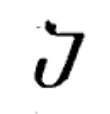
\includegraphics[scale=0.15]{images/georgianLetter.png}.\footnote{\translatorHD{Adjarian provides a Georgian letter 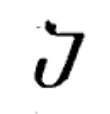
\includegraphics[scale=0.15]{images/georgianLetter.png} to signify the uvular stop. I don't know Georgian so I discussed the matter with David Erschler and Thomas Wier. Based on our discussion, the letter that Adjarian provided is probably a misprint because it doesn't exactly match an existing Georgian letter. It may have been a misprint of the letter for the sound /q\armenian{ʼ}/ (the letter q'ari; Mkhedruli <\armenian{ყ}>, Asomtavruli <\armenian{Ⴗ}>) or for the sound /q\textsuperscript{(}ʰ\textsuperscript{)}/ (the latter qari or khari; Mkhedruli <\armenian{ჴ}>). \label{footnote:georgian letter}}} It is pronounced as a strictly glottal /ʁ/ <\armenian{ղ}>, similar to the Arabic sound /q/.



\begin{table}[H]
	\centering
	\caption{Glottal /q/ <\armenian{ղՙ}> in the Tbilisi dialect }
	\label{tab:tbilisi:phonology:segment:q}
	\begin{tabular}{|lll| }
		\hline `from where' & vuɾqɑnt͡sʰ& \armenian{վուրղՙանց} \\
		`from here' & esqɑnt͡sʰ& \armenian{էսղՙանց} \\
		\hline 
	\end{tabular}
	
	
\end{table} 

As can be seen, the Tbilisi has almost completely preserved the phonetic richness of Old Armenian. But... 


\begin{adjarianpage}\label{page:53}\end{adjarianpage}% should be 53

... this is due to the influence of the Georgian language, such that all of the dialect's sounds bear the stamp of Georgian pronunciation. Especially the glottal pronunciation of the sounds /p k t t͡s t͡ʃ/ <\armenian{պ կ տ ծ ճ}> is Georgian. The sound /q/ <\armenian{ղՙ}>, as we know, is a pure borrowing from Georgian. The sound /f/ <\armenian{ֆ}>is absent in this dialect because it is also absent in Georgian. The same is for the sounds /œ, ʏ, æ/ <\armenian{էօ, իւ, ա̈}> . 



\subsection{Sound changes}
Among the phonetic changes of the Tbilisi dialect, whether limited or very general, the following are the characteristic ones for this dialect. 

\subsubsection{Monophthong vowels}
\paragraph{Classical Armenian /e/ <\armenian{ե}> }


Classical Armenian /e/ <\armenian{ե}> has become /ji/ <\armenian{յի}> when word-initial in monosyllabic words (Table \ref{tab:tbilisi:phono:change:EIniitalMono}). 


\begin{table}[H]
	\centering
	\caption{Change from word-initial monosyllabic CA /e/ <\armenian{ե}> to /ji/ <\armenian{յի}> in the Tbilisi dialect}
	\label{tab:tbilisi:phono:change:EIniitalMono}
	\begin{tabular}{|l|ll|ll|ll|}
		\hline & \multicolumn{2}{l|}{Classical Armenian}& \multicolumn{2}{l|}{> Tbilisi }& \multicolumn{2}{l|}{cf. SEA }
		\\
		`I' & es & \armenian{ես} & jis & \armenian{յիս} & jes & \armenian{ես} \\
		`when' & eɾb & \armenian{երբ} & jipʰ & \armenian{յիփ} & jeɾpʰ & \armenian{երբ} \\
		`ox' & ezən & \armenian{եզն} & jizɾ & \armenian{յիզր} & jez & \armenian{եզ} \\
		`oil' & eɬ & \armenian{եղ} & jiʁ & \armenian{յիղ} & juʁ & \armenian{յուղ} \\
		\hline
	\end{tabular}
	
\end{table}

At the beginning of polysyllabic words, this sound changed to /e/ <\armenian{է}> (Table \ref{tab:tbilisi:phono:change:EIniitalPoly}). 




\begin{table}[H]
	\centering
	\caption{Change from word-initial polysyllabic CA /e/ <\armenian{ե}> to /e/ <\armenian{է}> in the Tbilisi dialect}
	\label{tab:tbilisi:phono:change:EIniitalPoly}
	\begin{tabular}{|l|ll|ll|ll|}
		\hline & \multicolumn{2}{l|}{Classical Armenian}& \multicolumn{2}{l|}{> Tbilisi }& \multicolumn{2}{l|}{cf. SEA }
		\\
		`iron' & eɾk\'ɑtʰ & \armenian{երկաթ} & \'eɾkɑtʰ & \armenian{է՛րկաթ} & jeɾk\'ɑtʰ & \armenian{երկաթ} \\
		`face' & eɾ\'es & \armenian{երես} & \'eɾes & \armenian{է՛րէս} & jeɾ\'es & \armenian{երես} \\
		`two' & eɾk\'u & \armenian{երկու} & \'eɾku & \armenian{է՛րկու} & jeɾk\'u & \armenian{երկու} \\
		`dream' & eɾ\'ɑz & \armenian{երազ} & \'eɾɑz & \armenian{է՛րազ} & jeɾ\'ɑz & \armenian{երազ} \\
		`child' & eɾɑχ\'ɑi̯ & \armenian{երախայ} & eɾ\'eχɑ &\armenian{էրէ՛խա} & jeɾeχ\'ɑ & \armenian{երեխա} \\
		`sky' & eɾk\'in & \armenian{երկին} & \'eɾɡinkʰ & \armenian{է՛րգինք} & jeɾk\'iŋkʰ & \armenian{երկինք} \\
		\hline
	\end{tabular}
	
\end{table}

In the final syllable, meaning when it was stressed, the Classical /e/ <\armenian{ե}> becomes /i/ <\armenian{ի}> (Table \ref{tab:tbilisi:phono:change:EFinalStressed}).


\begin{table}[H]
	\centering
	\caption{Change from final CA /e/ <\armenian{ե}> to /i/ <\armenian{ի}> in the Tbilisi dialect}
	\label{tab:tbilisi:phono:change:EFinalStressed}
	\begin{tabular}{|l|ll|ll|ll|}
		\hline & \multicolumn{2}{l|}{Classical Armenian}& \multicolumn{2}{l|}{> Tbilisi }& \multicolumn{2}{l|}{cf. SEA }
		\\
		`place' & teɬ & \armenian{տեղ} & tiʁ & \armenian{տիղ} & teʁ & \armenian{տեղ} \\
		`night' & ɡiʃ\'eɾ & \armenian{գիշեր} & ɡ\'iʃiɾ & \armenian{գի՛շիր} & ɡiʃ\'eɾ & \armenian{գիշեր} \\
		`you' & kʰez & \armenian{քեզ} & kʰiz & \armenian{քիզ} & kʰez & \armenian{քեզ} \\
		`honey' & meɬəɾ & \armenian{մեղր} & miʁɾ & \armenian{միղր} & meʁəɾ & \armenian{մեղր} \\
		`seed' & seɾmən & \armenian{սերմն} & siɾm & \armenian{սիրմ} & seɾm & \armenian{սերմ} \\
		
		\hline
	\end{tabular}
\end{table}

But in preceding syllables, meaning before the stressed syllable, the vowel is /e/ <\armenian{է}> (Table \ref{tab:tbilisi:phono:change:EFinalPreStressed}).


\begin{table}[H]
	\centering
	\caption{Change from pre-tonic CA /e/ <\armenian{ե}> to /e/ <\armenian{է}> in the Tbilisi dialect}
	\label{tab:tbilisi:phono:change:EFinalPreStressed}
	\begin{tabular}{|l|ll|ll|ll|}
		\hline & \multicolumn{2}{l|}{Classical Armenian}& \multicolumn{2}{l|}{> Tbilisi }& \multicolumn{2}{l|}{cf. SEA }
		\\
		`to see' & tesɑn\'el & \armenian{տեսանել} & t\'esnil & \armenian{տէ՛սնիլ} & tesn\'el & \armenian{տեսնել} \\
		`to bring' & beɾ\'el & \armenian{բերել} & b\'eɾil &\armenian{բէ՛րիլ} & beɾ\'el & \armenian{բերել} \\
		
		
		\hline
	\end{tabular}
\end{table}


\paragraph{Classical Armenian /o/ <\armenian{ո}> }


Classical Armenian /o/ <\armenian{ո}> became /vu/ <\armenian{վու}> at the beginning of both monosyllabic and polysyllabic words (Table \ref{tab:tbilisi:phono:change:oInitial}).


\begin{table}[H]
	\centering
	\caption{Change word-initial CA /o/ <\armenian{ո}> to /vu/ <\armenian{վու}> in the Tbilisi dialect}
	\label{tab:tbilisi:phono:change:oInitial}
	\begin{tabular}{|l|ll|ll|ll|}
		\hline & \multicolumn{2}{l|}{Classical Armenian}& \multicolumn{2}{l|}{> Tbilisi }& \multicolumn{2}{l|}{cf. SEA }
		\\
		`orphan' & oɾb & \armenian{որբ} & vuɾpʰ & \armenian{վուրփ} & voɾpʰ & \armenian{որբ} \\
		`son' & oɾd\'i & \armenian{որդի} & v\'uɾtʰi & \armenian{վո՛ւրթի} & voɾtʰ\'i & \armenian{որդի} \\
		`that' & oɾ & \armenian{որ} & vuɾ & \armenian{վուր} & voɾ  & \armenian{որ} \\
		`foot' & otən & \armenian{ոտն} & vut & \armenian{վուտ} & votkʰ & \armenian{ոտք} \\
		`nothing' & ot͡ʃʰ\'int͡ʃʰ & \armenian{ոչինչ} & v\'unt͡ʃʰit͡ʃʰ & \armenian{վո՛ւնչիչ} & vot͡ʃʰ\'int͡ʃʰ & \armenian{ոչինչ} \\
		
		
		\hline
	\end{tabular}
\end{table}



In the final syllable, meaning under stress, the vowel becomes /u/ <\armenian{ու}> (Table \ref{tab:tbilisi:phono:change:oFinal}).


\begin{table}[H]
	\centering
	\caption{Change of final CA /o/ <\armenian{ո}> to /u/ <\armenian{ու}> in the Tbilisi dialect}
	\label{tab:tbilisi:phono:change:oFinal}
	\begin{tabular}{|l|ll|ll|ll|}
		\hline & \multicolumn{2}{l|}{Classical Armenian}& \multicolumn{2}{l|}{> Tbilisi }& \multicolumn{2}{l|}{cf. SEA }
		\\
		`work' & ɡoɾt͡s & \armenian{գործ}& ɡuɾd͡z & \armenian{գուրձ} & ɡoɾt͡s & \armenian{գործ} \\
		`belly' & pʰoɾ & \armenian{փոր}& pʰuɾ & \armenian{փուր} & pʰoɾ & \armenian{փոր} \\
		`smell' & hot & \armenian{հոտ}& hut & \armenian{հուտ} & hot & \armenian{հոտ} \\
		`four' & t͡ʃʰoɾs & \armenian{չորս}& t͡ʃʰuɾs & \armenian{չուրս} & t͡ʃʰoɾs & \armenian{չորս} \\
		`bosom' & t͡sot͡sʰ & \armenian{ծոց}& t͡sut͡sʰ & \armenian{ծուց} & t͡sot͡sʰ & \armenian{ծոց} \\
		`new' & noɾ & \armenian{նոր}& nuɾ & \armenian{նուր} & noɾ & \armenian{նոր} \\
		\hline
	\end{tabular}
\end{table}



In other syllables, it stays /o/ <\armenian{օ}> (Table \ref{tab:tbilisi:phono:change:oOther}).


\begin{table}[H]
	\centering
	\caption{Change of other positions of CA /o/ <\armenian{ո}> to /o/ <\armenian{օ}> in the Tbilisi dialect}
	\label{tab:tbilisi:phono:change:oOther}
	\resizebox{\textwidth}{!}{%
	\begin{tabular}{|l|ll|ll|ll|}
		\hline & \multicolumn{2}{l|}{Classical Armenian}& \multicolumn{2}{l|}{> Tbilisi }& \multicolumn{2}{l|}{cf. SEA }
		\\
		`barefoot' & bok\'ik & \armenian{բոկիկ}& b\'oblik & \armenian{բօ՛բլիկ} & bob\'ik & \armenian{բոբիկ} \\
		`to grow moldy' & boɾbosil & \armenian{բորբոսիլ}& boɾpʰsnil & \armenian{բօրփսնիլ} & boɾbosel & \armenian{բորբոսել} \\
		`to praise' & ɡov\'el & \armenian{գովել}& ɡ\'ovil & \armenian{գօ՛վիլ} & ɡov\'el & \armenian{գովել} \\
		\hline
	\end{tabular}
}
\end{table}


\subsubsection{Diphthongs }
\paragraph{Classical Armenian /oi̯/ <\armenian{ոյ}>}

Classical Armenian /oi̯/ <\armenian{ոյ}> becomes /u/ <\armenian{ու}> (Table \ref{tab:tbilisi:phono:change:oj}).


\begin{table}[H]
	\centering
	\caption{Change of CA /oi̯/ <\armenian{ոյ}> to /u/ <\armenian{ու}> in the Tbilisi dialect}
	\label{tab:tbilisi:phono:change:oj}
	\begin{tabular}{|l|ll|ll|ll|}
		\hline & \multicolumn{2}{l|}{Classical Armenian}& \multicolumn{2}{l|}{> Tbilisi }& \multicolumn{2}{l|}{cf. SEA }
		\\
		`light' & loi̯s & \armenian{լոյս}& lus & \armenian{լուս} & lujs & \armenian{լույս} \\
		`sister' & kʰoi̯ɾ & \armenian{քոյր}& kʰuɾ & \armenian{քուր} & kʰujɾ & \armenian{քույր} \\
		`sweet' & ɑn\'oi̯ʃ & \armenian{անոյշ}& \'ɑnuʃ & \armenian{ա՛նուշ} & ɑn\'ujʃ (dated) & \armenian{անույշ} \\
		& & & & & ɑn\'uʃ & \armenian{անուշ} \\
		`color' & ɡoi̯n-kʰ (plural) & \armenian{գոյնք}& ɡunkʰ & \armenian{գունք} & ɡujn & \armenian{գույն} \\
		\hline
	\end{tabular}
\end{table}



\paragraph{Classical Armenian /iu̯/ <\armenian{իւ}>}

Classical Armenian /iu̯/ <\armenian{իւ}> became /u/ <\armenian{ու}> (Table \ref{tab:tbilisi:phono:change:iu}).%\footnote{\translatorHD{For `weaved', Adjarian provides an ancestor <\armenian{հիւսած}>. But it's unclear to me if this form is attested in Classical Armenian, so as an ancestor I show the infinitive <\armenian{հիւսել}>.}}

\begin{table}[H]
	\centering
	\caption{Change of CA /iu̯/ <\armenian{իւ}> to /u/ <\armenian{ու}> in the Tbilisi dialect}
	\label{tab:tbilisi:phono:change:iu}
	\begin{tabular}{|l|ll|ll|ll|}
		\hline & \multicolumn{2}{l|}{Classical Armenian}& \multicolumn{2}{l|}{> Tbilisi }& \multicolumn{2}{l|}{cf. SEA }
		\\
		`blood' & ɑɾ\'iu̯n & \armenian{արիւն}& \'ɑɾun & \armenian{ա՛րուն} & ɑɾj\'un & \armenian{արյուն} \\
		`flour' & ɑl\'iu̯ɾ & \armenian{ալիւր}& \'ɑluɾ & \armenian{ա՛լուր} & ɑlj\'uɾ & \armenian{ալյուր} \\
		`hundred' & hɑɾ\'iu̯ɾ & \armenian{հարիւր}& h\'ɑɾuɾ & \armenian{հա՛րուր} & hɑɾj\'uɾ & \armenian{հարյուր} \\
		`to weave' & hiu̯s\'el & \armenian{հիւսել}& & & hjus\'el & \armenian{հյուսել} \\
		`weaved' & & & h\'usɑt͡s & \armenian{հո՛ւսած} & hjus\'ɑt͡s & \armenian{հյուսած} \\
		`guest' & hiu̯ɾ & \armenian{հիւր}& huɾ & \armenian{հուր} & hjuɾ & \armenian{հյուր} \\
		`snow' & d͡ziu̯n & \armenian{ձիւն}& d͡zun & \armenian{ձուն} & d͡zjun & \armenian{ձյուն} \\
		`branch' & t͡ʃiu̯ɬ & \armenian{ճիւղ}& t͡ʃuχk & \armenian{ճուխկ} & t͡ʃjuʁ & \armenian{ճյուղ} \\
		\hline
	\end{tabular}
\end{table}
\subsubsection{Consonant changes}
\paragraph{Stops and affricates }

For the three degrees of consonants, although the dialect has in general preserved the old sources, but in some places the sounds have gotten confused with each other. Let us cite some examples of these special cases (Table \ref{tab:tbilisi:phono:change:voicing}). 


\begin{table}[H]
	\centering
	\caption{Sporadic laryngeal changes of stops in the Tbilisi dialect}
	\label{tab:tbilisi:phono:change:voicing}
	\resizebox{\textwidth}{!}{%
	\begin{tabular}{|l|ll|ll|ll|}
		\hline & \multicolumn{2}{l|}{Classical Armenian}& \multicolumn{2}{l|}{> Tbilisi }& \multicolumn{2}{l|}{cf. SEA }
		\\
		`to find' & ɡətɑnel & \armenian{գտանել}& ɡtʰnil & \armenian{գթնիլ} & ɡətnel & \armenian{գտնել} \\
		`courtyard' & bɑk & \armenian{բակ}& bɑɡ & \armenian{բագ} & bɑk & \armenian{բակ} \\
		`sun' & ɑɾeɡ\'ɑkən & \armenian{արեգակն}& ɑɾ\'eɡɑɡ & \armenian{արէ՛գագ} & ɑɾeɡ\'ɑk & \armenian{արեգակ} \\
		`sky' & eɾk\'in-kʰ (plural) & \armenian{երկինք}& \'eɾɡinkʰ & \armenian{է՛րգինք} & jeɾk\'iŋkʰ & \armenian{երկինք} \\
		`land' & eɾk\'iɾ & \armenian{երկիր}& \'eɾɡiɾ & \armenian{է՛րգիր}& jeɾk\'iɾ & \armenian{երկիր} \\
		`I know' & ɡit\'em & \armenian{գիտեմ}& ɡ\'idim & \armenian{գի՛դիմ}& ɡit\'em & \armenian{գիտեմ} \\
		`with' & het & \armenian{հետ}& hid & \armenian{հիդ} & het& \armenian{հետ} \\
		`to respect' & met͡sɑɾ\'el & \armenian{մեծարել}& m\'ed͡zɾil & \armenian{մէ՛ձրիլ} & met͡sɑɾ\'el& \armenian{մեծարել} \\
		`ground' & ɡet\'in & \armenian{գետին}& ɡ\'edin & \armenian{գէ՛դին} & ɡet\'in& \armenian{գետին} \\
		`work' & ɡoɾt͡s & \armenian{գործ}& ɡuɾd͡z & \armenian{գուրձ} & ɡoɾt͡s& \armenian{գործ} \\
		\hline
	\end{tabular}
}
\end{table}


\paragraph{Post-nasal voicing}
As a general, all voiceless consonants become voiced after the nasal /n/ <\armenian{ն}> (Table \ref{tab:tbilisi:phono:change:postvoicing}). 


\begin{table}[H]
	\centering
	\caption{Post-nasal voicing in the Tbilisi dialect}
	\label{tab:tbilisi:phono:change:postvoicing}
	\resizebox{\textwidth}{!}{%
	\begin{tabular}{|l|ll|ll|ll|}
		\hline & \multicolumn{2}{l|}{Classical Armenian}& \multicolumn{2}{l|}{> Tbilisi }& \multicolumn{2}{l|}{cf. SEA }
		\\
		`to plant' & tənkel & \armenian{տնկել}& tnɡil & \armenian{տնգիլ} & təŋkel & \armenian{տնկել} \\
		`ear' & ɑk\'ɑnd͡ʒ & \armenian{ականջ}& \'ɑnɡɑt͡ʃ & \armenian{ա՛նգաճ} & ɑk\'ɑnd͡ʒ & \armenian{ականջ} \\
		`free, ownerless' & ɑnt\'eɾ & \armenian{անտէր}& \'ɑndeɾ & \armenian{ա՛նդէր} & ɑnt\'eɾ & \armenian{անտեր} \\
		`friend' & ənkeɾ & \armenian{ընկեր}& nənɡiɾ & \armenian{նընգիր} & əŋkeɾ & \armenian{ընկեր} \\
		`woman (nominative)' & & & knik & \armenian{կնիկ} & kənik & \armenian{կնիկ} \\
		`woman (genitive)' & & & knɡɑ & \armenian{կնգա} & kəŋkɑn & \armenian{կնկան} \\
		\hline
	\end{tabular}
}
\end{table}

\paragraph{Nasal epenthesis}

For the sound sequence /ənɡ/ <\armenian{ընգ}> in the Tbilisi dialect, there is an also an initial \armenian{ն} /n/ (Table \ref{tab:tbilisi:phono:change:nasalEPen}). 


\begin{table}[H]
	\centering
	\caption{Nasal epenthesis in the Tbilisi dialect}
	\label{tab:tbilisi:phono:change:nasalEPen}
	\resizebox{\textwidth}{!}{%
	\begin{tabular}{|l|ll|ll|ll|}
		\hline & \multicolumn{2}{l|}{Classical Armenian}& \multicolumn{2}{l|}{> Tbilisi }& \multicolumn{2}{l|}{cf. SEA }
		\\
		`friend' & ənkeɾ & \armenian{ընկեր}& nənɡiɾ & \armenian{նընգիր} & əŋkeɾ & \armenian{ընկեր} \\
		`walnut-tree' & ənkuzeni & \armenian{ընկուզենի}& nənɡzi & \armenian{նընգզի} & əŋkuzeni & \armenian{ընկուզենի} \\
		`to fall' & ɑnkɑnil & \armenian{անկանիլ}& nənɡnil & \armenian{նընգնիլ} & əŋknel& \armenian{ընկնել} \\
		\hline
	\end{tabular}
}
\end{table}



\begin{adjarianpage}\label{page:54}\end{adjarianpage}% should be 54

\paragraph{Change from /h/ <\armenian{հ}> to /χ/ <\armenian{խ}> }

The CA sound /h/ <\armenian{հ}>  is unchanged. But it has turned to /χ/ <\armenian{խ}> in only the words in Table \ref{tab:tbilisi:phono:change:hx}. 


\begin{table}[H]
	\centering
	\caption{Change from CA /h/ <\armenian{հ}> to /χ/ <\armenian{խ}> in the Tbilisi dialect}
	\label{tab:tbilisi:phono:change:hx}
	\begin{tabular}{|l|ll|ll|ll|}
		\hline & \multicolumn{2}{l|}{Classical Armenian}& \multicolumn{2}{l|}{> Tbilisi }& \multicolumn{2}{l|}{cf. SEA }
		\\
		`earth' & hoɬ & \armenian{հող}& χuʁ & \armenian{խուղ} & hoʁ & \armenian{հող} \\
		`to bless' & ɑu̯ɾhnel & \armenian{աւրհնել}& oχnil & \armenian{օխնիլ} & oɾhnel & \armenian{օրհնել} \\
		\hline
	\end{tabular}
\end{table}

\subsection{Stress}

Stress has moved from the last syllable to the penultimate syllable, as in the Yerevan dialect.

\section{Morphology}

\subsection{Noun inflection or declension}

The Tbilisi dialect has 7 cases, which are in general the same as in the Yerevan dialect, in both form and composition. The following are the main differences for the Tbilisi dialect:
\begin{itemize}
	\item The ablative uses the formative /eme, emen/ <\armenian{էմէ, էմէն}> (Table \ref{tab:tbilisi:morpho:noun:abl}). 
	
	
	\begin{table}[H]
		\centering
		\caption{Ablative suffix as /eme/ <\armenian{էմէ}> in the Tbilisi dialect}
		\label{tab:tbilisi:morpho:noun:abl}
		\resizebox{\textwidth}{!}{%
			\begin{tabular}{|l|ll|ll|ll|}
			\hline & \multicolumn{2}{l|}{Tbilisi }& \multicolumn{2}{l|}{cf. Yerevan }& \multicolumn{2}{l|}{cf. SEA }
			\\
			`from writing' & ɡɾ-emen & \armenian{գրէմէն}& ɡɾ-it͡sʰ & \armenian{գրից} & ɡəɾ-it͡sʰ & \armenian{գրից} \\
			`from house' & tn-emen & \armenian{տնէմէն}& tən-it͡sʰ & \armenian{տնից} & tən-it͡sʰ & \armenian{տնից} \\
			`from death' & mɑh-emen & \armenian{մահէմէն}& mɑh-it͡sʰ & \armenian{մահից} & mɑh-it͡sʰ & \armenian{մահից} \\
			\hline
		\end{tabular}
	}
	\end{table}
	
	
	\item The nominative plural is formed with the formatives /iɾ, niɾ/ <\armenian{իր, նիր}>. But the other cases keep the sound /e/ <\armenian{է}>, according to the phonetic rules. 
	\item The plural genitive takes the formative /-u/ <\armenian{ու}>, similar to the /kə/ <\armenian{կը}> branch dialects. 
\end{itemize}

The following is the declension of the word /div/ <\armenian{դիվ}> from Classical /deu̯/ <\armenian{դեւ}> `demon'. \translatorHD{I suspect that the final /n/ in all the words in Table \ref{tab:Tbilisi:morpho:noun} is actually a separate definite suffix /-n/, but I'm not sure. }

\begin{table}[H]
	\caption{Paradigm for noun inflection of the word /div/ <\armenian{դիվ}> `demon' in the Tbilisi dialect }\label{tab:Tbilisi:morpho:noun}
	\centering \begin{tabular}{|l|ll|ll|}
		\hline & \multicolumn{2}{l|}{Singular}& \multicolumn{2}{l|}{Plural} \\
		\hline {\nom} ({\acc}) & div & \armenian{դիվ} & div-iɾ & \armenian{դիվիր} \\
		{\gen} & div-i & \armenian{դիվի} & div-eɾ-u & \armenian{դիվէրու} \\
		{\dat} ({\acc}) & div-i, div-in & \armenian{դիվի, դիվին} & div-eɾ-u-(n) & \armenian{դիվէրու(ն}) \\
		{\abl} & div-emen & \armenian{դիվէմէն} & div-eɾ-emen & \armenian{դիվէրէմէն} \\
		{\ins} & div-ov & \armenian{դիվօվ} & div-er-ov & \armenian{դիվէրօվ} \\
		{\locgloss} & div-um & \armenian{դիվում} & div-er-um & \armenian{դիվէրում} 
		\\ \hline 
	\end{tabular}
\end{table}

\subsection{Pronoun inflection or declension}

The pronoun declensions are as follows. 

\translatorHD{Table \ref{tab:Tbilisi:morpho:pronoun:personal} is for personal pronouns. }

\begin{table}[H]
	\caption{Inflection paradigm for personal pronouns in the Tbilisi dialect }\label{tab:Tbilisi:morpho:pronoun:personal}
	\centering
	\resizebox{\textwidth}{!}{%
	\begin{tabular}{|l|lll|lll|}
		\hline & 1SG & 2SG & 3SG & 1PL & 2PL & 3PL \\
		& `I' & `you' & `he/she' & `we'& `you' & `they'\\\hline 
		{\nom} & jis & du & nɑ & minkʰ & dukʰ & nɾɑnkʰ \\
		& \armenian{յիս} & \armenian{դու} & \armenian{նա} & \armenian{մինք} & \armenian{դուք} & \armenian{նրանք} \\
		\hline {\gen} & im & kʰu & nɾɑ & miɾ & d͡ziɾ & nɾɑnt͡sʰ \\
		& \armenian{իմ} & \armenian{քու} & \armenian{նրա} & \armenian{միր} & \armenian{ձիր} & \armenian{նրանց} \\
		\hline {\dat},{\acc} & ind͡zi & kʰiz & nɾɑn & miz & d͡ziz & nɾɑnt͡sʰ \\
		& \armenian{ինձի} & \armenian{քիզ} & \armenian{նրան} & \armenian{միզ} & \armenian{ձիզ} & \armenian{նրանց} \\
		\hline {\abl} & ind͡z-m-en & kʰiz-m-en & nɾɑ-m-en & miz-m-en & d͡ziz-m-en & nɾɑnt͡sʰ-m-en \\
		& \armenian{ինձմէն} & \armenian{քիզմէն} & \armenian{նրամէն} & \armenian{միզմէն} & \armenian{ձիզմէն} & \armenian{նրանցմէն} \\
		\hline {\ins} & ind͡z-m-ov & kʰiz-m-ov & nɾɑn-ov & miz-m-ov & d͡ziz-m-ov & nɾɑnt͡sʰ-ov \\
		& \armenian{ինձմօվ} & \armenian{քիզմօվ} & \armenian{նրանօվ} & \armenian{միզմօվ} & \armenian{ձիզմօվ} & \armenian{նրանցօվ} \\
		\hline {\locgloss} & ind͡z-(ɑ)n-um & kʰiz-(ɑ)n-um & nrɑn-um & miz-(ɑ)n-um & d͡ziz-(ɑ)n-um & nɾɑnt͡sʰ-um \\
		& \armenian{ինձ(ա)նում} & \armenian{քիզ(ա)նում} & \armenian{նրանում} & \armenian{միզ(ա)նում} & \armenian{ձիզ(ա)նում} & \armenian{նրանցում} 
		\\ \hline 
	\end{tabular}
}
\end{table}

\begin{adjarianpage}\label{page:55}\end{adjarianpage}% should be 55

\translatorHD{Table \ref{tab:Tbilisi:morpho:pronoun:dem} is for demonstrative pronouns. }

\begin{table}[H]
	\caption{Inflection paradigm for demonstrative pronouns in the Tbilisi dialect }\label{tab:Tbilisi:morpho:pronoun:dem}
	\centering
		\resizebox{\textwidth}{!}{%
		 \begin{tabular}{|l|lll|lll|}
		\hline & \multicolumn{3}{c|}{Singular}& \multicolumn{3}{c|}{Plural}
		\\ 
		& proximal & medial & distal & proximal & medial & distal \\
		& `this' & `that' & `that yonder' & `these' & `those' & `those yonder' \\ \hline
		{\nom} & es & et & en & estunkʰ & etunkʰ & endunkʰ \\
		& \armenian{էս} & \armenian{էտ} & \armenian{էն} & \armenian{էստունք} & \armenian{էտունք} & \armenian{էնդունք} \\\hline
		{\gen}, {\dat} & estu & etu & endu & estunt͡sʰ & etunt͡sʰ & endunt͡sʰ \\
		& \armenian{էստու} & \armenian{էտու} & \armenian{էնդու} & \armenian{էստունց} & \armenian{էտունց} & \armenian{էնդունց} \\\hline
		{\abl} & estu-men & etu-men & endu-men & estunt͡sʰ-men & etunt͡sʰ-men & endunt͡sʰ-men \\
		& \armenian{էստումէն} & \armenian{էտումէն} & \armenian{էնդումէն} & \armenian{էստունցմէն} & \armenian{էտունցմէն} & \armenian{էնդունցմէն} \\\hline
		{\ins} & est-ov & et-ov & end-ov & estunt͡sʰ-ov & etunt͡sʰ-ov & endunt͡sʰ-ov \\
		& \armenian{էստօվ} & \armenian{էտօվ} & \armenian{էնդօվ} & \armenian{էստունցօվ} & \armenian{էտունցօվ} & \armenian{էնդունցօվ} \\\hline
		{\locgloss} & est-um & et-um & end-um & estunt͡sʰ-um & etunt͡sʰ-um & endunt͡sʰ-um \\
		& \armenian{էստում} & \armenian{էտում} & \armenian{էնդում} & \armenian{էստունցում} & \armenian{էտունցում} & \armenian{էնդունցում} 
		\\ \hline
	\end{tabular}
}
\end{table}

\translatorHD{Table \ref{tab:Tbilisi:morpho:pronoun:ink} is for the logophoric third person pronoun. }

\begin{table}[H]
	\caption{Inflection paradigm for demonstrative pronouns in the Tbilisi dialect }\label{tab:Tbilisi:morpho:pronoun:ink}
	\centering \begin{tabular}{|l|ll|ll|}
		\hline & \multicolumn{2}{l|}{3SG} & \multicolumn{2}{l|}{3PL} \\\hline 
		{\nom} & inkʰə & \armenian{ինքը} & iɾɑnkʰ & \armenian{իրանք} \\
		{\gen} & iɾ(ɑ) & \armenian{իր(ա}) & iɾɑnt͡sʰ & \armenian{իրանց} \\
		{\dat},{\acc} & iɾɑn & \armenian{իրան} & iɾɑnt͡sʰ & \armenian{իրանց} \\
		{\abl} & iɾ-men & \armenian{իրմէն} & iɾɑnt͡sʰ-men & \armenian{իրանցմէն} \\
		{\ins} & iɾ-m-ov & \armenian{իրմօվ} & iɾɑnt͡sʰ-m-ov & \armenian{իրանցմօվ} \\
		{\locgloss} & iɾɑn-um & \armenian{իրանում} & iɾɑnt͡sʰ-um & \armenian{իրանցում} \\ \hline 
	\end{tabular}
\end{table}

\subsection{Verb inflection or conjugation}

\subsubsection{Various aspects of verb inflection}
\paragraph{Sound changes for verbal vowels}
The verbs are conjuated in the manner of Yerevan, except for the required phonetic changes. For example, for the copula verb in the present, the Classical sounds /e, ē/ <\armenian{ե, է}> become   /i/ <\armenian{ի}> for all the persons (except for the third). And because of this, the stem of the verb uses the endings /-um im, -um is/ <-\armenian{ում իմ}, -\armenian{ում իս}>. 

\translatorHD{These points are illustrated later in \S\ref{section:Tbilisi:morpho:verb:paradigm:indcPresPst}.}

\paragraph{Irregular imperfective converb for monosyllabic verbs}

Like the Yerevan dialect, the monosyllabic verbs take the formative /-is/ <\armenian{իս}> (Table \ref{tab:Tbilisi:morpho:verb:imperfIrregIs}). 



\begin{table}[H]
	\centering
	\caption{Irregular imperfective converbs for monosyllabic verbs with /-is/ in the Tbilisi dialect }
	\label{tab:Tbilisi:morpho:verb:imperfIrregIs}
	
	\begin{tabular}{|l|ll|ll| }
		\hline & \multicolumn{2}{l|}{Tbilisi }& \multicolumn{2}{l|}{cf. SEA } \\
		\hline Infinitive &&& \multicolumn{2}{l|}{$\sqrt{}$-{\thgloss}-{\infgloss}} \\
		`to come' & & & ɡ-ɑ-l & \armenian{գալ} \\
		`to give' & & & t-ɑ-l & \armenian{տալ} \\
		`to cry' & & & l-ɑ-l & \armenian{լալ} \\
		\hline Present 1SG & \multicolumn{4}{l|}{$\sqrt{}$-{\thgloss}-{\infgloss}-{\impfcvb} {\aux}-1{\sg}} \\
		`I come' & ɡ-\'ɑ-l-is e-m & \armenian{գա՛լիս էմ} & ɡ-ɑ-l-is e-m & \armenian{գալիս եմ} \\
		`I give' & t-\'ɑ-l-is e-m & \armenian{տա՛լիս էմ} & t-ɑ-l-is e-m & \armenian{տալիս եմ} \\
		`I cry' & l-\'ɑ-l-is e-m & \armenian{լա՛լիս էմ} & l-ɑ-l-is e-m & \armenian{լալիս եմ} \\
		\hline 
	\end{tabular} 
\end{table}

\paragraph{Lack of /e/ deletion before past /-i/}\label{sec:Tbilisi:morpho:verb:various:eImpf}


In the imperfective, the reflex of the Classical sound /ē/ <\armenian{է}> does not shorten. The forms are pronounced as in Old Armenian  (Table \ref{tab:Tbilisi:morpho:verb:pastaux}, \ref{tab:Tbilisi:morpho:verb:imperf}). \translatorHD{What he means is that unlike in the Yerevan dialect, the auxiliary /e/ and theme vowel /e/ do not delete before the past suffix /-i/. The Tbilisi dialect thus patterns with SEA in this regard.} 



\begin{table}[H]
	\centering
	\caption{Past auxiliary in the Tbilisi dialect }
	\label{tab:Tbilisi:morpho:verb:pastaux}
	
	\begin{tabular}{|l|ll|ll| }
		\hline & \multicolumn{2}{l|}{Tbilisi }& \multicolumn{2}{l|}{cf. SEA } \\
	1SG	`I was' & e-i-$\emptyset$ & \armenian{էի} &  ej-i-$\emptyset$ & \armenian{էի} \\
	2SG	 `you were' & e-i-ɾ & \armenian{էիր} &  ej-i-ɾ & \armenian{էիր} \\
				3SG  `he was' & e-$\emptyset$-ɾ & \armenian{էր} &  e-$\emptyset$-ɾ & \armenian{էր} \\
1PL	 `we were' & e-i-nkʰ & \armenian{էինք} &  ej-i-ŋkʰ & \armenian{էինք} \\
	2PL	  `you were' & e-i-kʰ & \armenian{էիք} &  ej-i-kʰ & \armenian{էիք} \\
	3PL `they were'	  & e-i-n & \armenian{էին} &  ej-i-n & \armenian{էին} \\
					& \multicolumn{2}{l|}{{\aux}-{\pst}-{\agr} }			& \multicolumn{2}{l|}{{\aux}-{\pst}-{\agr} }\\
		\hline 
	\end{tabular} 
\end{table}



\begin{table}[H]
	\centering
	\caption{Indicative past imperfective in the Tbilisi dialect }
	\label{tab:Tbilisi:morpho:verb:imperf}
	
	\begin{tabular}{|l|ll|ll| }
		\hline & \multicolumn{2}{l|}{Tbilisi }& \multicolumn{2}{l|}{cf. SEA } \\
		`I was speaking' & χos-um e-i-$\emptyset$ & \armenian{խօսում էի} & χos-um ej-i-$\emptyset$ & \armenian{խոսում էի} \\
		`I was saying' & ɑs-um e-i-$\emptyset$ & \armenian{ասում էի} & ɑs-um ej-i-$\emptyset$ & \armenian{ասում էի} \\
		& \multicolumn{2}{l|}{$\sqrt{}$-{\impfcvb} {\aux}-{\pst}-1{\sg} }& \multicolumn{2}{l|}{$\sqrt{}$-{\impfcvb} {\aux}-{\pst}-1{\sg} } \\
		\hline 
	\end{tabular} 
\end{table}




\begin{adjarianpage}\label{page:56}\end{adjarianpage}% should be 56

\paragraph{Allomorphy of the future formative /ku/ <\armenian{կու}>}

The future formative is /ku/ <\armenian{կու}> instead of /kə/ <\armenian{կը}> (Table \ref{tab:Tbilisi:morpho:verb:futKU}).\footnote{\translatorHD{Some modern grammars of SEA treat the formative /k/ as as a conditional future marker \citep[253ff]{DumTragut-2009-ArmenianReferenceGrammar}. But to maintain consistency with Adjarian, I gloss it as a future marker. I likewise faithfully translate his terms   for the tenses that use this formative. } }



\begin{table}[H]
	\centering
	\caption{Future formative as /ku/ <\armenian{կու}> in the Tbilisi dialect }
	\label{tab:Tbilisi:morpho:verb:futKU}
	
	\begin{tabular}{|l|ll|ll| }
		\hline & \multicolumn{2}{l|}{Tbilisi }& \multicolumn{2}{l|}{cf. SEA } \\
		`I will like' & ku siɾ-i-m & \armenian{կու սիրիմ} & kə-siɾ-e-m & \armenian{կսիրեմ} \\
		`I will bring' & ku beɾ-i-m & \armenian{կու բէրիմ} & kə-beɾ-e-m & \armenian{կբերեմ} \\
		& \multicolumn{2}{l|}{{\fut}-$\sqrt{}$-{\thgloss}-1{\sg} }& \multicolumn{2}{l|}{{\fut}-$\sqrt{}$-{\thgloss}-1{\sg} } \\
		\hline 
	\end{tabular} 
\end{table}

Before vowel-initial verbs, this particle is sometimes shortened to \armenian{կ} /k/, but a lot of times it stays constant (Table \ref{tab:Tbilisi:morpho:verb:imperfIrregIs}). 



\begin{table}[H]
	\centering
	\caption{Variable shortening of the future formative as /ku/ <\armenian{կու}> before vowel-initial verbs in the Tbilisi dialect }
	\label{tab:Tbilisi:morpho:verb:futKConst}
	
	\begin{tabular}{|l|ll|ll| }
		\hline & \multicolumn{2}{l|}{Tbilisi }& \multicolumn{2}{l|}{cf. SEA } \\
		? & k-eh-ɑ-m & \armenian{կէհամ} & & \\
		`I will go' & k-eɾtʰ-ɑ-m & \armenian{կէրթամ} & k-eɾtʰ-ɑ-m & \armenian{կերթամ} \\
		`I will have' & k-unen-ɑ-m & \armenian{կունէնամ} & k-eɾtʰ-ɑ-m & \armenian{կունենամ} \\
		`I will free' & ku ɑzɑt-i-m & \armenian{կու ազատիմ} & k-ɑzɑt-e-m & \armenian{կազատեմ} \\
		`I will pray' & ku ɑʁotʰ-i-m & \armenian{կու աղօթիմ} & k-ɑʁotʰ-e-m & \armenian{կաղոթեմ} \\
		`I will burn' & ku eɾ-i-m & \armenian{կու էրիմ} & k-ɑjɾ-e-m & \armenian{կայրեմ} \\
		`I will know' & ku imɑn-ɑ-m & \armenian{կու իմանամ} & k-ɑjɾ-ɑ-m & \armenian{կիմանամ} \\
		& \multicolumn{2}{l|}{{\fut}-$\sqrt{}$-{\thgloss}-1{\sg} }& \multicolumn{2}{l|}{{\fut}-$\sqrt{}$-{\thgloss}-1{\sg} } \\
		`I will take' & ku ɑr-n-i-m & \armenian{կու առնիմ} & k-ɑr-n-e-m & \armenian{կառնեմ} \\
		& \multicolumn{2}{l|}{{\fut}-$\sqrt{}$-{\vx}-{\thgloss}-1{\sg} }& \multicolumn{2}{l|}{{\fut}-$\sqrt{}$-{\vx}-{\thgloss}-1{\sg} } \\
		
		\hline 
	\end{tabular} 
\end{table}

The particle becomes voiced /ɡ/ <\armenian{գ}> before the verb `to want' (Table \ref{tab:Tbilisi:morpho:verb:imperfIrregIs}). 



\begin{table}[H]
	\centering
	\caption{Voicing of the future formative as /ɡ/ <\armenian{գ}> for the verb `to want' in the Tbilisi dialect }
	\label{tab:Tbilisi:morpho:verb:futKG}
	
	\resizebox{\textwidth}{!}{%
	\begin{tabular}{|l|ll|ll|l| }
		\hline & \multicolumn{2}{l|}{Tbilisi }& \multicolumn{2}{l|}{cf. SEA } & \\
		`I will want' & ɡ-uz-i-m & \armenian{գուզիմ} & k-uz-e-m & \armenian{կուզեմ} & {\fut}-$\sqrt{}$-{\thgloss}-1{\sg} \\
		`you will want' & ɡ-uz-i-s & \armenian{գուզիս} & k-uz-e-s & \armenian{կուզես} & {\fut}-$\sqrt{}$-{\thgloss}-2{\sg} \\
		`I was wanting' & ɡ-uz-e-i-$\emptyset$ & \armenian{գուզէի} & k-uz-e-s & \armenian{կուզես} & {\fut}-$\sqrt{}$-{\thgloss}-{\pst}-1{\sg} \\
		
		
		\hline 
	\end{tabular} 
}
\end{table}

It is also voiced as in Table \ref{tab:Tbilisi:morpho:verb:futKgu}. \translatorHD{Note that he doesn't state what is the root of these verbs. So I segment the prefix as /ɡu/ based on the contrast against SEA, but Adjarian might have meant that the prefix as /ɡ-/ while the verb was /ukʰɑm/.}



\begin{table}[H]
	\centering
	\caption{Voicing of the future formative as /ɡ(u?)/ <\armenian{գու}> for the verb `to come' in the Tbilisi dialect }
	\label{tab:Tbilisi:morpho:verb:futKgu}
	
	\begin{tabular}{|l|ll|ll|l| }
		\hline & \multicolumn{2}{l|}{Tbilisi }& \multicolumn{2}{l|}{cf. SEA } & \\
		`I will come' & ɡu-kʰ-ɑ-m & \armenian{գուքամ} & kə-ɡ-ɑ-m & \armenian{կգամ} & {\fut}-$\sqrt{}$-{\thgloss}-1{\sg} \\
		`you will come' & ɡu-kʰ-ɑ-s & \armenian{գուքաս} & kə-ɡ-ɑ-s & \armenian{կգաս} & {\fut}-$\sqrt{}$-{\thgloss}-2{\sg} \\
		\hline 
	\end{tabular} 
\end{table}


Before the verbs in Table\ref{tab:Tbilisi:morpho:verb:futKCoales}, the particle is fused with the /ɑ/ <\armenian{ա}>, and becomes /ko/ <\armenian{կօ}>. 



\begin{table}[H]
	\centering
	\caption{Coalesence of merger of the future formative /ku/ <\armenian{կու}> and verb-initial /ɑ/ <\armenian{ա}> as /ko/ <\armenian{կօ}> in the Tbilisi dialect }
	\label{tab:Tbilisi:morpho:verb:futKCoales}
	
	\begin{tabular}{|l|ll|ll| }
		\hline & \multicolumn{2}{l|}{Tbilisi }& \multicolumn{2}{l|}{cf. SEA } \\
		\hline Infinitive && &\multicolumn{2}{l|}{$\sqrt{}$-{\thgloss}-{\infgloss}} \\
		`to lay' & & &ɑt͡s-e-l & \armenian{ածել} \\
		`to do'& & &ɑn-e-l & \armenian{անել} \\
		`to say' & & &ɑs-e-l & \armenian{ասել} \\
		\hline Future 1{\sg} &\multicolumn{2}{l|}{{\fut}-$\sqrt{}$-{\thgloss}-1{\sg}} &\multicolumn{2}{l|}{{\fut}-$\sqrt{}$-{\thgloss}-1{\sg}} \\
		`I will lay &k-ot͡s-i-m &\armenian{կօծիմ} &k-ɑt͡s-e-m & \armenian{կածեմ} \\
		`I will do' &k-on-i-m &\armenian{կօնիմ} &k-ɑn-e-m & \armenian{կանեմ} \\
		`I will say' &k-os-i-m & \armenian{կօսիմ} & k-ɑs-e-m & \armenian{կասեմ} \\
		\hline Past future 1{\sg} &\multicolumn{2}{l|}{{\fut}-$\sqrt{}$-{\thgloss}-{\pst}-1{\sg}} &\multicolumn{2}{l|}{{\fut}-$\sqrt{}$-{\thgloss}-{\pst}-1{\sg}} \\
		`I was going to lay &k-ot͡s-e-i-$\emptyset$ &\armenian{կօծէի} &k-ɑt͡s-ej-i-$\emptyset$ & \armenian{կածեի} \\
		`I was going to do' &k-on-e-i-$\emptyset$ &\armenian{կօնէի} &k-ɑn-ej-i-$\emptyset$ & \armenian{կանեի} \\
		`I was going to say' &k-os-e-i-$\emptyset$ & \armenian{կօսէի} & k-ɑs-ej-i-$\emptyset$ & \armenian{կասեի} \\
		\hline 
	\end{tabular} 
\end{table}

\paragraph{Past participle or perfective converb with /-il,-i/ <\armenian{իլ, ի}> }

The past participle has the ending /-il/ <\armenian{իլ}>. This is used to form the present perfect (\armenian{յարակատար}), past perfect (\armenian{գերակատար}), and the negative (\armenian{բացասական}) forms (Table \ref{tab:Tbilisi:morpho:verb:pastPart}). 



\begin{table}[H]
	\centering
	\caption{Past participle or perfective converb with /-il/ <\armenian{իլ}> in the Tbilisi dialect }
	\label{tab:Tbilisi:morpho:verb:pastPart}
		\resizebox{\textwidth}{!}{% 
	\begin{tabular}{|l|ll|ll|l| }
		\hline & \multicolumn{2}{l|}{Tbilisi }& \multicolumn{2}{l|}{cf. SEA } & \\
		`I have liked' & siɾ-il i-m & \armenian{սիրիլ իմ} & siɾ-el e-m & \armenian{սիրել եմ} & $\sqrt{}$-{\perfcvb} {\aux}-1{\sg} \\
		`I had liked' & siɾ-il e-i-$\emptyset$ & \armenian{սիրիլ էի} & siɾ-el ej-i-$\emptyset$ & \armenian{սիրել էի} & $\sqrt{}$-{\perfcvb} {\aux}-{\pst}-1{\sg} \\
		\hline 
	\end{tabular} 
}
\end{table}

But when the auxiliary is before the participle, the last letter of the suffix is lost (Table \ref{sent:Tbilisi:morpho:verb:pastPartMove}). 


\begin{exe}
	\ex Tbilisi dialect \label{sent:Tbilisi:morpho:verb:pastPartMove} \begin{xlist}
		\ex \gll t͡ʃʰ-i-m siɾ-i \\
		{\neggloss}-{\aux}-1{\sg} like-{\perfcvb} \\
		\trans `I have not liked.' \\
		\armenian{չիմ սիրի}
		\ex \gll jis i-m beɾ-i \\
		I {\aux}-1{\sg} bring-{\perfcvb} \\
		\trans `\textbf{I} have brought (as opposed to someone else).' \\
		\armenian{յիս իմ բէրի}
	\end{xlist}
\end{exe}
\subsubsection{General paradigm}

Here we show the most often used forms of the verb `to like', as a reflex from Classical /siɾ-e-l/ <\armenian{սիրել}>. 


{\paradigmExplanation}

\paragraph{Indicative present and past imperfective}\label{section:Tbilisi:morpho:verb:paradigm:indcPresPst}

\translatorHD{The indicative present in SEA is formed via periphrasis (Table \ref{tab:Tbilisi:morpho:verb:paradigm:presentIndc}). The verb is in a converb form called the imperfective converb with the suffix /-um/. Tense and agreement is on an inflected auxiliary. The Tbilisi dialect shows the same strategy with one major difference. The auxiliary /e/ is replaced by /i/ for all but the present 3SG. }


\begin{table}[H]
	\centering
	\caption{Indicative present <\armenian{ներկայ}> of the verb `to like' in the Tbilisi dialect}
	\label{tab:Tbilisi:morpho:verb:paradigm:presentIndc}
	\begin{tabular}{|l|ll|ll|}
		\hline & \multicolumn{2}{l|}{Tbilisi} & \multicolumn{2}{l|}{cf. SEA} \\
		1SG & siɾ-um i-m & \armenian{սիրում իմ} & siɾ-um e-m & \armenian{սիրում եմ} \\
		2SG & siɾ-um i-s & \armenian{սիրում իս} & siɾ-um e-s & \armenian{սիրում ես} \\
		3SG & siɾ-um e & \armenian{սիրում է} & siɾ-um e & \armenian{սիրում է} \\
		1PL & siɾ-um i-nkʰ & \armenian{սիրում ինք} & siɾ-um e-ŋkʰ & \armenian{սիրում ենք}\\
		2PL & siɾ-um i-kʰ & \armenian{սիրում իք} & siɾ-um e-kʰ & \armenian{սիրում եք} \\
		3PL & siɾ-um i-n & \armenian{սիրում ին} & siɾ-um e-n & \armenian{սիրում են} \\
		& \multicolumn{2}{l|}{$\sqrt{}$-{\impfcvb} {\aux}-{\agr}}& \multicolumn{2}{l|}{$\sqrt{}$-{\impfcvb} {\aux}-{\agr}}
		\\ \hline 
\end{tabular} \end{table}



\translatorHD{The indicative past imperfective uses the same imperfective converb as in the present (Table \ref{tab:Tbilisi:morpho:verb:paradigm:pastImpfIndc}). The difference is that auxiliary is now in the past tense. In both SEA and Tbilisi, the auxiliary has the shape /e/.}



\begin{table}[H]
	\centering
	\caption{Indicative past imperfective <\armenian{անկատար}> of the verb `to like' in the Tbilisi dialect}
	\label{tab:Tbilisi:morpho:verb:paradigm:pastImpfIndc}
	\begin{tabular}{|l|ll|ll|}
		\hline & \multicolumn{2}{l|}{Tbilisi} & \multicolumn{2}{l|}{cf. SEA} \\
		1SG & siɾ-um e-i-$\emptyset$ & \armenian{սիրում էի} & siɾ-um ej-i-$\emptyset$ & \armenian{սիրում էի} \\
		2SG & siɾ-um e-i-ɾ & \armenian{սիրում էիր} & siɾ-um ej-i-ɾ & \armenian{սիրում էիր} \\
		3SG & siɾ-um e-$\emptyset$-ɾ & \armenian{սիրում էր} & siɾ-um e-$\emptyset$-ɾ & \armenian{սիրում էր} \\
		1PL & siɾ-um e-i-nkʰ & \armenian{սիրում էինք} & siɾ-um ej-i-ŋkʰ & \armenian{սիրում էինք} \\
		2PL & siɾ-um e-i-kʰ & \armenian{սիրում էիք} & siɾ-um ej-i-kʰ & \armenian{սիրում էիք} \\
		3PL & siɾ-um e-i-n & \armenian{սիրում էին} & siɾ-um ej-i-n & \armenian{սիրում էին} \\
		& \multicolumn{2}{l|}{$\sqrt{}$-{\impfcvb} {\aux}-{\pst}-{\agr}}& \multicolumn{2}{l|}{$\sqrt{}$-{\impfcvb} {\aux}-{\pst}-{\agr}} \\
		\hline 
	\end{tabular}
\end{table}

\translatorHD{Thus in Tbilisi, the auxiliary shows variation in its morphs: /e/ for some inflection cells, while /i/ for other cells. See \S\ref{sec:Tbilisi:morpho:verb:various:eImpf}.}


\paragraph{Present perfect and past perfect}

\translatorHD{The present perfect (Table \ref{tab:Tbilisi:morpho:verb:paradigm:presentPerfect}) and past perfect (Table \ref{tab:Tbilisi:morpho:verb:paradigm:pastPerfect}) in SEA are formed with periphrasis. The verb is in the form of the perfective converb with the suffix /-el/. The present tense auxiliary is added for the present perfect, while the past auxiliary for the past perfect. The Tbilisi dialect essentially uses the same strategy but with two differences. First, the converb suffix is /-il/ not /-el/. Second, the auxiliary shows the same changes in its shape as for the indicative present and past. }

\begin{table}[H]
	\centering
	\caption{Present perfect <\armenian{յարակատար}> of the verb `to like' in the Tbilisi dialect}
	\label{tab:Tbilisi:morpho:verb:paradigm:presentPerfect}
	\begin{tabular}{|l|ll|ll|}
		\hline & \multicolumn{2}{l|}{Tbilisi} & \multicolumn{2}{l|}{cf. SEA} \\
		1SG & siɾ-il i-m & \armenian{սիրիլ իմ} & siɾ-el e-m & \armenian{սիրել եմ} \\
		2SG & siɾ-il i-s & \armenian{սիրիլ իս} & siɾ-el e-s & \armenian{սիրել ես} \\
		3SG & siɾ-il e & \armenian{սիրիլ է} & siɾ-el e & \armenian{սիրել է} \\
		1PL & siɾ-il i-nkʰ & \armenian{սիրիլ ինք} & siɾ-el e-ŋkʰ & \armenian{սիրել ենք} \\
		2PL & siɾ-il i-kʰ & \armenian{սիրիլ իք} & siɾ-el e-kʰ & \armenian{սիրել եք} \\
		3PL & siɾ-il i-n & \armenian{սիրիլ ին} & siɾ-el e-n & \armenian{սիրել են} \\
		& \multicolumn{2}{l|}{$\sqrt{}$-{\perfcvb} {\aux}-{\agr}}& \multicolumn{2}{l|}{$\sqrt{}$-{\perfcvb} {\aux}-{\agr}}\\ 
		
		\hline 
	\end{tabular}
\end{table}

\begin{table}[H]
	\centering
	\caption{Past perfect <\armenian{գերակատար}> of the verb `to like' in the Tbilisi dialect}
	\label{tab:Tbilisi:morpho:verb:paradigm:pastPerfect}
	\begin{tabular}{|l|ll|ll| }
		\hline & \multicolumn{2}{l|}{Tbilisi} & \multicolumn{2}{l|}{cf. SEA} \\
		1SG & siɾ-il e-i-$\emptyset$ & \armenian{սիրիլ էի} & siɾ-el ej-i-$\emptyset$ & \armenian{սիրել էի} \\
		2SG & siɾ-il e-i-ɾ & \armenian{սիրիլ էիր} & siɾ-el ej-i-ɾ & \armenian{սիրել էիր} \\
		3SG & siɾ-il e-$\emptyset$-ɾ & \armenian{սիրիլ էր} & siɾ-el e-$\emptyset$-ɾ & \armenian{սիրել էր} \\
		1PL & siɾ-il e-i-nkʰ & \armenian{սիրիլ էինք} & siɾ-el ej-i-ŋkʰ & \armenian{սիրել էինք} \\
		2PL & siɾ-il e-i-kʰ & \armenian{սիրիլ էիք} & siɾ-el ej-i-kʰ & \armenian{սիրել էիք} \\
		3PL & siɾ-il e-i-n & \armenian{սիրիլ էին} & siɾ-el ej-i-n & \armenian{սիրել էին} \\
		& \multicolumn{2}{l|}{$\sqrt{}$-{\perfcvb} {\aux}-{\pst}-{\agr}}& \multicolumn{2}{l|}{$\sqrt{}$-{\perfcvb} {\aux}-{\pst}-{\agr}}\\ 
		
		\hline 
	\end{tabular}
\end{table}

\paragraph{Past perfective or aorist}

\translatorHD{The past perfective (Table \ref{tab:Tbilisi:morpho:verb:paradigm:pastperfectiveAorist}) is also called the aorist. In SEA for /siɾ-e-l/ `to like', the past perfective is formed by taking the root and theme vowel, adding the aorist or perfective suffix /-t͡sʰ-/, and then adding the past suffix /-i/ and the appropriate agreement suffixes. The 3SG uses covert tense and agreement suffixes. The Tbilisi dialect behaves the same, though the 3SG uses a different theme vowel. }


\begin{table}[H]
	\centering
	\caption{Past perfective or aorist <\armenian{կատարեալ}> of the verb `to like' in the Tbilisi dialect}
	\label{tab:Tbilisi:morpho:verb:paradigm:pastperfectiveAorist}
	\begin{tabular}{|l|ll|ll|}
		\hline & \multicolumn{2}{l|}{Tbilisi} & \multicolumn{2}{l|}{cf. SEA} \\
		1SG & siɾ-e-t͡sʰ-i-$\emptyset$ & \armenian{սիրէցի} & siɾ-e-t͡sʰ-i-$\emptyset$ & \armenian{սիրեցի} \\
		2SG & siɾ-e-t͡sʰ-i-ɾ & \armenian{սիրէցիր} & siɾ-e-t͡sʰ-i-ɾ & \armenian{սիրեցիր} \\
		3SG & siɾ-i-t͡sʰ-$\emptyset$-$\emptyset$ & \armenian{սիրից} & siɾ-e-t͡sʰ-$\emptyset$-$\emptyset$ & \armenian{սիրեց} \\
		1PL & siɾ-e-t͡sʰ-i-nkʰ & \armenian{սիրէցինք} & siɾ-e-t͡sʰ-i-ŋkʰ & \armenian{սիրեցինք} \\
		2PL & siɾ-e-t͡sʰ-i-kʰ & \armenian{սիրէցիք} & siɾ-e-t͡sʰ-i-kʰ & \armenian{սիրեցիք} \\
		3PL & siɾ-e-t͡sʰ-i-n & \armenian{սիրէցին} & siɾ-e-t͡sʰ-i-n & \armenian{սիրեցին} \\
		& \multicolumn{2}{l|}{$\sqrt{}$-{\thgloss}-{\aor}-{\pst}-{\agr}}& \multicolumn{2}{l|}{$\sqrt{}$-{\thgloss}-{\aor}-{\pst}-{\agr}}\\ 
		
		\hline 
	\end{tabular}
\end{table}



\paragraph{Subjunctive present and past } 

\translatorHD{In SEA, the subjunctive present (Table \ref{tab:Tbilisi:morpho:verb:paradigm:subjPresent}) is formed by adding agreement suffixes after the theme vowel. These are the same agreement suffixes that are added onto the present auxiliary in the indicative present. For a verb like `to like', the 3SG involves changing the theme vowel /e/ to /i/ in the 3SG. The Tbilisi dialect follows the same system but with the opposite choice of vowels. The theme vowel is /e/ for the present 3SG, and /i/ elsewhere. } 


\begin{table}[H]
	\centering
	\caption{Subjunctive present <\armenian{ստորադասական ներկայ}> of the verb `to like' in the Tbilisi dialect}
	\label{tab:Tbilisi:morpho:verb:paradigm:subjPresent}
	\begin{tabular}{|l|ll|ll|}
		\hline & \multicolumn{2}{l|}{Tbilisi} & \multicolumn{2}{l|}{cf. SEA} \\
		1SG & siɾ-i-m & \armenian{սիրիմ} & siɾ-e-m & \armenian{սիրեմ} \\
		2SG & siɾ-i-s & \armenian{սիրիս} & siɾ-e-s & \armenian{սիրես} \\
		3SG & siɾ-e-$\emptyset$ & \armenian{սիրէ} & siɾ-i-$\emptyset$ & \armenian{սիրի} \\
		1PL & siɾ-i-nkʰ & \armenian{սիրինք} & siɾ-e-ŋkʰ & \armenian{սիրենք} \\
		2PL & siɾ-i-k & \armenian{սիրիք} & siɾ-e-k & \armenian{սիրեք} \\
		3PL & siɾ-i-n & \armenian{սիրին} & siɾ-e-n & \armenian{սիրեն} \\
		& \multicolumn{2}{l|}{$\sqrt{}$-{\thgloss}-{\agr}}& \multicolumn{2}{l|}{$\sqrt{}$-{\thgloss}-{\agr}}\\ 
		
		\hline 
	\end{tabular}
\end{table}

\translatorHD{In SEA, the subjunctive past (Table \ref{tab:Tbilisi:morpho:verb:paradigm:subjPast}) is formed by adding the past suffix /i/ and agreement suffixes after the theme vowel. In Tbilisi, the same is used. Note how the theme vowel stays a constant /e/ in the past, unlike the variation in the present. }



\begin{table}[H]
	\centering
	\caption{Subjunctive past <\armenian{ստորադասական անցեալ}> of the verb `to like' in the Tbilisi dialect}
	\label{tab:Tbilisi:morpho:verb:paradigm:subjPast}
	\begin{tabular}{|l|ll|ll|}
		\hline & \multicolumn{2}{l|}{Tbilisi} & \multicolumn{2}{l|}{cf. SEA} \\
		1SG & siɾ-e-i-$\emptyset$ & \armenian{սիրէի} & siɾ-ej-i-$\emptyset$ & \armenian{սիրեի} \\
		2SG & siɾ-e-i-ɾ & \armenian{սիրէիր} & siɾ-ej-i-ɾ & \armenian{սիրեիր} \\
		3SG & siɾ-e-$\emptyset$-ɾ & \armenian{սիրէր} & siɾ-e-$\emptyset$-ɾ & \armenian{սիրեր} \\
		1PL & siɾ-e-i-nkʰ & \armenian{սիրէինք} & siɾ-ej-i-nkʰ & \armenian{սիրեինք} \\
		2PL & siɾ-e-i-kʰ & \armenian{սիրէիք} & siɾ-ej-i-kʰ & \armenian{սիրեիք} \\ 
		3PL & siɾ-e-i-n & \armenian{սիրէին} & siɾ-ej-i-n & \armenian{սիրեին} \\ 
		& \multicolumn{2}{l|}{$\sqrt{}$-{\thgloss}-{\pst}-{\agr}}& \multicolumn{2}{l|}{$\sqrt{}$-{\thgloss}-{\pst}-{\agr}}\\ 
		
		\hline 
	\end{tabular}
\end{table}

\paragraph{Tenses built from the subjunctive: Future and debitive}


\translatorHD{In Tbilisi, many other tenses seem to be built off of the subjunctive (Table \ref{tab:Tbilisi:morpho:verb:paradigm:complexSubjunctive}). The future and past future are built by adding the prefix /ku/ before the subjunctive present and subjunctive past. The debitive and debitive past are formed also by adding the proclitic /piti/ before the appropriate subjunctive form. I don't provide morpheme glosses for these forms for space. SEA behaves essentially the same (with the expected difference in theme vowels) and I don't provide its paradigm. }


\begin{table}[H]
	\centering
	\caption{Forms that are built from the subjunctive forms for the verb `to like' in the Tbilisi dialect}
	\label{tab:Tbilisi:morpho:verb:paradigm:complexSubjunctive}
	\begin{tabular}{|l|ll|ll|}
		\hline & 
		\multicolumn{2}{l|}{Future <\armenian{ապառնի}>} & \multicolumn{2}{l|}{Past future <\armenian{անցեալ ապառնի}> } \\
		 1SG & ku siɾ-i-m & \armenian{կու սիրիմ} & ku siɾ-e-i-$\emptyset$ & \armenian{կու սիրէի} \\
		2SG & ku siɾ-i-s & \armenian{կու սիրիս} & ku siɾ-e-i-ɾ & \armenian{կու սիրէիր} \\
		3SG & ku siɾ-e-$\emptyset$ & \armenian{կու սիրէ} & ku siɾ-e-$\emptyset$-ɾ & \armenian{կու սիրէր} \\
		1PL & ku siɾ-i-nkʰ & \armenian{կու սիրինք} & ku siɾ-e-i-nkʰ & \armenian{կու սիրէինք} \\
		2PL & ku siɾ-i-k & \armenian{կու սիրիք} & ku siɾ-e-i-kʰ & \armenian{կու սիրէիք} \\
		3PL & ku siɾ-i-n & \armenian{կու սիրին} & ku siɾ-e-i-n & \armenian{կու սիրէին} \\
		& \multicolumn{2}{l|}{{\fut} $\sqrt{}$-{\thgloss}-{\agr}}& \multicolumn{2}{l|}{{\fut} $\sqrt{}$-{\thgloss}-{\pst}-{\agr}}
		\\ \hline 
		& \multicolumn{2}{l|}{Debitive  } & \multicolumn{2}{l|}{Debitive past } \\
		& \multicolumn{2}{l|}{\armenian{պարտաւորական ներկայ} } & \multicolumn{2}{l|}{\armenian{պարտաւորական անցեալ} } \\
				1SG & piti siɾ-i-m & \armenian{պիտի սիրիմ} & piti siɾ-e-i-$\emptyset$ & \armenian{պիտի սիրէի} \\
		2SG & piti siɾ-i-s & \armenian{պիտի սիրիս} & piti siɾ-e-i-ɾ & \armenian{պիտի սիրէիր} \\
		3SG & piti siɾ-e-$\emptyset$ & \armenian{պիտի սիրէ} & piti siɾ-e-$\emptyset$-ɾ & \armenian{պիտի սիրէր} \\
		1PL & piti siɾ-i-nkʰ & \armenian{պիտի սիրինք} & piti siɾ-e-i-nkʰ & \armenian{պիտի սիրէինք} \\
		2PL & piti siɾ-i-k & \armenian{պիտի սիրիք} & piti siɾ-e-i-kʰ & \armenian{պիտի սիրէիք} \\
		3PL & piti siɾ-i-n & \armenian{պիտի սիրին} & piti siɾ-e-i-n & \armenian{պիտի սիրէին} \\ 
		& \multicolumn{2}{l|}{{\deb} $\sqrt{}$-{\thgloss}-{\agr}}& \multicolumn{2}{l|}{{\deb} $\sqrt{}$-{\thgloss}-{\pst}-{\agr}}
		\\\hline \end{tabular}
\end{table}
 

\translatorHD{The debitive forms show an alternative strategy. The previously discussed strategy in Table \ref{tab:Tbilisi:morpho:verb:paradigm:complexSubjunctive} was to place the particle /piti/ before the inflected verb. The verb carries tense and agreement inflection. In contrast, an alternative strategy (Table \ref{tab:Tbilisi:morpho:verb:paradigm:debitiveOther}) is to place the tense and agreement morphology onto the particle /piti/. The verb is then in a constant shape: /siɾ-i/ for `to like'. Agreement is thus mobile.}

\begin{table}[H]
	\centering
	\caption{Alternative forms for the debitive for the verb `to like' in the Tbilisi dialect with mobile agreement}
	\label{tab:Tbilisi:morpho:verb:paradigm:debitiveOther}
	\begin{tabular}{|l|ll|ll|}
		\hline 
		& \multicolumn{2}{l|}{Debitive  } & \multicolumn{2}{l|}{Debitive past } \\
& \multicolumn{2}{l|}{\armenian{պարտաւորական ներկայ} } & \multicolumn{2}{l|}{\armenian{պարտաւորական անցեալ} } \\

		1SG & pit-i-m siɾ-i & \armenian{պիտիմ սիրի} & pit-e-i-$\emptyset$ siɾ-i & \armenian{պիտէի սիրի} \\
		2SG & pit-i-s siɾ-i & \armenian{պիտիս սիրի} & pit-e-i-ɾ siɾ-i & \armenian{պիտէիր սիրի} \\
		3SG & pit-i-$\emptyset$ siɾ-i & \armenian{պիտի սիրի} & pit-e-$\emptyset$-ɾ siɾ-i & \armenian{պիտէր սիրի} \\
		1PL & pit-i-nk siɾ-i & \armenian{պիտինք սիրի} & pit-e-i-nk siɾ-i & \armenian{պիտէինք սիրի} \\
		2PL & pit-i-kʰ siɾ-i & \armenian{պիտիք սիրի} & pit-e-i-kʰ siɾ-i & \armenian{պիտէիք սիրի} \\
		3PL & pit-i-n siɾ-i & \armenian{պիտին սիրի} & pit-e-i-n siɾ-i & \armenian{պիտէին սիրի} \\
		& \multicolumn{2}{l|}{{\deb}-?-{\agr} $\sqrt{}$-? }& \multicolumn{2}{l|}{{\deb}-?-{\pst}-{\agr} $\sqrt{}$-? }
		\\\hline \end{tabular}
\end{table}


\translatorHD{Adjarian doesn't ambiguously state if the verb in this alternative strategy is a specific participle, or if all verbs show the same type of final vowel. It's also unclear to me what is the proper glossing for the inflected forms of the particle /piti/. The second vowel alternates between /i,e/ in exactly the same way as the theme vowel of the verb `to' like' in the above paradigms. It's unclear to me if the second vowel in this particle is thus still the same debitive morpheme, vs. a theme vowel, vs.   some other morpheme. }


\paragraph{Other tenses built from participles}

\translatorHD{Adjarian provides a paradigm for something he calls the `debitive past perfect'. It consists of the debitive particle /piti/, plus what appears to be the perfective converb with /-il/, and then the past auxiliary. }


\begin{table}[H]
	\centering
	\caption{Debitive past perfective <\armenian{պարտաւորական գերակատար}> for the verb `to like' in the Tbilisi dialect}
	\label{tab:Tbilisi:morpho:verb:paradigm:debitivePerf}
	\begin{tabular}{|l|ll|}
		\hline 
		1SG & piti siɾ-il e-i-$\emptyset$ & \armenian{պիտի սիրիլ էի} \\
		2SG & piti siɾ-il e-i-ɾ & \armenian{պիտի սիրիլ էիր} \\
		3SG & piti siɾ-il e-$\emptyset$-ɾ & \armenian{պիտի սիրիլ էր} \\
		1PL & piti siɾ-il e-i-nkʰ & \armenian{պիտի սիրիլ էինք} \\
		2PL & piti siɾ-il e-i-kʰ & \armenian{պիտի սիրիլ էիք} \\
		3PL & piti siɾ-il e-i-n & \armenian{պիտի սիրիլ էին} \\ 
		& \multicolumn{2}{l|}{{\deb} $\sqrt{}$-{\perfcvb} {\aux}-{\pst}-{\agr} }
		\\\hline \end{tabular}
\end{table}

\paragraph{Imperative and prohibitive}

\translatorHD{For the imperative 2SG, SEA adds the morph /-iɾ/ after the root for a verb like `to like' (Table \ref{tab:Tbilisi:morpho:verb:paradigm:Imp}). For the 2PL, archaic SEA adds the sequence /-e-t͡sʰ-ekʰ/ after the root such that /-e-t͡sʰ/ forms the aorist stem, while /-ekʰ/ is the agreement marker. More modern registers use just the suffix /-ekʰ/ without the aorist stem. The prohibitive is marked by just adding the proclitic /mi/ before the verb}

\translatorHD{Tbilisi uses the same strategy for the imperative 2PL. For the 2SG, the post-root vowel is /e/. It's unclear if this /e/ is a special agrement morpheme or if it's the theme vowel. For the prohibitive though, Tbilisi ends up using /i/ for the 2SG, and /ekʰ/ for the 2PL. Thus the imperative and negative imperative (prohibitive) are not obviously connected. }


\begin{table}[H]
	\centering
	\caption{Imperative and negative imperative forms <\armenian{հրամայական}> for the verb `to like' in the Tbilisi dialect}
	\label{tab:Tbilisi:morpho:verb:paradigm:Imp}
	\resizebox{\textwidth}{!}{%
	\begin{tabular}{|l|ll|lll|l|}
		\hline & \multicolumn{2}{l|}{Tbilisi} & \multicolumn{3}{l|}{cf. SEA} & \\\hline
		{\imp} 2SG & siɾ-\'e & \armenian{սիրէ՛} & siɾ-iɾ & \armenian{սիրիր} & & $\sqrt{}$-{\imp}.2{\sg}\\
		{\imp} 2PL & siɾ-e-t͡sʰ-ekʰ & \armenian{սիրէցէք} & siɾ-e-t͡sʰ-ekʰ & \armenian{սիրեցեք} & dated & $\sqrt{}$-{\thgloss}-{\aor}-{\imp}.2{\pl} \\
		& & & siɾ-ekʰ & \armenian{սիրեք} & modern& $\sqrt{}$-{\imp}.2{\pl} \\ \hline 
		{\proh} 2SG & m\'i siɾ-i & \armenian{մի՛ սիրի} & mi siɾ-iɾ & \armenian{մի սիրիր} & & {\proh} $\sqrt{}$-{\imp}.2{\sg} \\
		{\proh} 2PL & & & mi siɾ-e-t͡sʰ-ekʰ & \armenian{մի սիրեցեք} & dated & {\proh} $\sqrt{}$-{\thgloss}-{\aor}-{\imp}.2{\pl} \\
		& m\'i siɾ-ekʰ & \armenian{մի սիրէք} & mi siɾ-ekʰ & \armenian{մի սիրեք} & modern
		& {\proh} $\sqrt{}$-{\imp}.2{\pl} 
		\\\hline \end{tabular}
}
\end{table}


\paragraph{Non-finite forms}

\translatorHD{Finally, Adjarian lists the following non-finite forms of this verb (participles or converbs) in Table \ref{tab:Tbilisi:morpho:verb:paradigm:participle}. Note that present participle is also called the subject participle. What Adjarian calls the past participle is differentiated in SEA as a resultative participle with /-ɑt͡s/ and a perfective converb with /-el/.} 

\begin{table}[H]
	\centering
	\caption{Participles or converbs <\armenian{դերբայներ}> for the verb `to like' in the Tbilisi dialect}
	\label{tab:Tbilisi:morpho:verb:paradigm:participle}
	\resizebox{\textwidth}{!}{%
	\begin{tabular}{|ll|ll|ll|l|}
		\hline & & \multicolumn{2}{l|}{Tbilisi} & \multicolumn{2}{l|}{cf. SEA} & \\
		Infinitive& \armenian{անորոշ} & siɾ-i-l & \armenian{սիրիլ} & siɾ-e-l & \armenian{սիրել} & $\sqrt{}$-{\thgloss}-{\infgloss} \\
		Present & \armenian{ներկայ} & siɾ-oʁ & \armenian{սիրօղ} & siɾ-oʁ &\armenian{սիրող} & $\sqrt{}$-{\sptcp} \\
		Past & \armenian{անցեալ} & siɾ-il & \armenian{սիրիլ} & siɾ-el & \armenian{սիրել} & $\sqrt{}$-{\perfcvb} \\
		& & siɾ-i & \armenian{սիրի}& && $\sqrt{}$-{\perfcvb} 
		\\
		& & siɾ-ɑt͡s & \armenian{սիրած} & siɾ-ɑt͡s & \armenian{սիրած} & $\sqrt{}$-{\rptcp} \\
		Future & \armenian{ապառնի} & siɾ-e-l-u & \armenian{սիրէլու} & siɾ-e-l-u & \armenian{սիրելու} & $\sqrt{}$-{\thgloss}-{\infgloss}-{\futcvb} \\
		& & siɾ-e-l-ɑt͡sʰu & \armenian{սիրէլացու} & & & $\sqrt{}$-{\thgloss}-{\infgloss}-? 
		\\\hline \end{tabular}
	}
\end{table}

\begin{adjarianpage}\label{page:57}\end{adjarianpage}% should be 57

\subsubsection{Other conjugation classes}

The other conjugations follow this pattern for the most part. The present, imperfective, and the future use the same strategy. It is only the past perfective and the imperative which have their own construction, in accordance with Classical Armenian.

\translatorHD{He means that the past perfective and imperative have class-specific construction rules, similar to CA and to SEA. Table \ref{tab:Tbilisi:morpho:verb:otherClass:aorist:ICLass} shows the paradigm for the I-Class. The I-Class with theme /-i-/ does not exist in SEA, but it does in SWA. For easier contrast, we contrast Tbilisi with SWA. }


\begin{table}[H]
	\centering
	\caption{Past perfectives (aorists) and imperatives for the I-Class verb /-il/ <\armenian{իլ}> `to live' in the Tbilisi dialect}
	\label{tab:Tbilisi:morpho:verb:otherClass:aorist:ICLass}
	\resizebox{\textwidth}{!}{%
\begin{tabular}{|l|ll|ll|}
		\hline & \multicolumn{2}{l|}{Tbilisi} & \multicolumn{2}{l|}{cf. SWA} \\ \hline 
		Infinitive & & &\multicolumn{2}{l|}{$\sqrt{}$-{\thgloss}-{\infgloss}} \\
		& & & ɑbɾ-i-l & \armenian{ապրիլ} \\ \hline 
		Past perfective & \multicolumn{2}{l|}{$\sqrt{}$-{\thgloss}-{\aor}-{\pst}-{\agr}} & \multicolumn{2}{l|}{$\sqrt{}$-{\thgloss}-{\aor}-{\pst}-{\agr}}\\
		1SG & ɑpɾ-e-t͡sʰ-ɑ-$\emptyset$ &\armenian{ապրէցա} & ɑbɾ-e-t͡sʰ-ɑ-$\emptyset$ & \armenian{ապրեցայ} \\
		2SG & ɑpɾ-e-t͡sʰ-ɑ-ɾ &\armenian{ապրէցար} & ɑbɾ-e-t͡sʰ-ɑ-ɾ & \armenian{ապրեցար} \\
		3SG & ɑpɾ-e-t͡sʰ-ɑ-v &\armenian{ապրէցավ}& ɑbɾ-e-t͡sʰ-ɑ-v & \armenian{ապրեցաւ} \\
		1PL & ɑpɾ-e-t͡sʰ-ɑ-nkʰ &\armenian{ապրէցանք}& ɑbɾ-e-t͡sʰ-ɑ-ŋkʰ & \armenian{ապրեցանք} \\
		2PL & ɑpɾ-e-t͡sʰ-ɑ-kʰ &\armenian{ապրէցաք}& ɑbɾ-e-t͡sʰ-ɑ-kʰ & \armenian{ապրեցաք} \\
		3PL & ɑpɾ-e-t͡sʰ-ɑ-n &\armenian{ապրէցան}& ɑbɾ-e-t͡sʰ-ɑ-nʰ & \armenian{ապրեցան} \\
		\hline 
		Imperative & \multicolumn{2}{l|}{$\sqrt{}$-{\thgloss}-({\aor})-{\agr}} & \multicolumn{2}{l|}{$\sqrt{}$-{\thgloss}-({\aor})-{\agr}}\\
		2SG & ɑpɾ-\'i-$\emptyset$ &\armenian{ապրի՛} & ɑbɾ-i-ɾ & \armenian{ապրիր} \\
		2PL & ɑpɾ-e-t͡sʰ-ekʰ &\armenian{ապրէցէք}& ɑbɾ-e-t͡sʰ-ɑ-kʰ & \armenian{ապրեցէք} \\\hline 
		Prohibitive & \multicolumn{2}{l|}{{\proh} $\sqrt{}$-{\thgloss}?-{\agr}} & \multicolumn{2}{l|}{{\proh} $\sqrt{}$-{\thgloss}-{\agr}}\\
		2SG & m\'i ɑpɾ-\'i-$\emptyset$ & \armenian{մի՛ ապրի} &mi ɑbɾ-i-ɾ &\armenian{մի ապրիր} \\
		2PL & m\'i ɑpɾ-e-kʰ &\armenian{մի՛ ապրէք}& mi ɑbɾ-i-kʰ & \armenian{մի ապրիք} \\
		\hline \end{tabular}
	}
\end{table}

\translatorHD{Another class is the irregular infixed verbs that end in the morph sequence /-n-i-l/. The /n/ is a meaningless stem-extender that's deleted in the past perfective. In SEA, the theme vowel /i/ is replaced by /e/. We show just the Tbilisi and SWA paradigms for illustration (Table \ref{tab:Tbilisi:morpho:verb:otherClass:aorist:infix}). }



\begin{table}[H]
	\centering
	\caption{Past perfectives (aorists) and imperatives for the infixed verb /hɑs-/ `to reach' and /hɑkʰ-/ `to wear' in the Tbilisi dialect}
	\label{tab:Tbilisi:morpho:verb:otherClass:aorist:infix}
	\resizebox{\textwidth}{!}{%
	\begin{tabular}{|l|ll|ll|}
		\hline & \multicolumn{2}{l|}{Tbilisi} & \multicolumn{2}{l|}{cf. SWA} \\ \hline \hline 
		Infinitive & & & \multicolumn{2}{l|}{$\sqrt{}$-{\vx}-{\thgloss}-{\infgloss}} \\
		& & & hɑs-n-i-l & \armenian{հասնիլ} \\ \hline 
		Past perfective & \multicolumn{2}{l|}{$\sqrt{}$-{\pst}-{\agr}} & \multicolumn{2}{l|}{$\sqrt{}$-{\pst}-{\agr}}\\
		1SG & hɑs-ɑ-$\emptyset$ &\armenian{հասա} & hɑs-ɑ-$\emptyset$ & \armenian{հասայ} \\
		2SG & hɑs-ɑ-ɾ &\armenian{հասար}& hɑs-ɑ-ɾ & \armenian{հասար} \\
		3SG & hɑs-ɑ-v &\armenian{հասավ}& hɑs-ɑ-v & \armenian{հասաւ} \\
		\hline \hline 
		Infinitive & & & \multicolumn{2}{l|}{$\sqrt{}$-{\vx}-{\thgloss}-{\infgloss}} \\
		& & & hɑkʰ-n-i-l & \armenian{հագնիլ} \\ \hline 
		Imperative & \multicolumn{2}{l|}{$\sqrt{}$-{\thgloss}-({\aor})-{\agr}} & \multicolumn{2}{l|}{$\sqrt{}$-{\thgloss}-({\aor})-{\agr}}\\
		2SG & hɑkʰ-\'i-$\emptyset$ &\armenian{հաքի՛} & hɑkʰ-i-ɾ & \armenian{հագիր} \\
		2PL & hɑkʰ-\'ekʰ &\armenian{հաքէ՛ք}& hɑkʰ-\'ekʰ & \armenian{հագէք} \\ \hline
		Prohibitive & \multicolumn{2}{l|}{{\proh} $\sqrt{}$-{\vx}-{\thgloss}?-{\agr}} & \multicolumn{2}{l|}{{\proh} $\sqrt{}$-{\vx}-{\thgloss}-{\agr}}\\
		2SG & m\'i hɑkʰ-n-\'i-$\emptyset$ & \armenian{մի՛ հաքնի} &mi hɑkʰ-n-i-ɾ &\armenian{մի հագնիր} \\
		2PL & m\'i hɑkʰ-n-e-kʰ &\armenian{մի՛ հաքնէք}& mi hɑkʰ-n-i-kʰ & \armenian{մի հագնիք} \\
		\hline \end{tabular}
	}
\end{table}

\translatorHD{The A-Class uses the theme /-ɑ/ and it's found in both SEA and Tbilisi. The two dialects utilize the same strategies for the perfective and imperative. Though in the prohibitive, SEA just uses the particle /mi/ plus the imperative, while Tbilisi uses the particle and a different sequence of verbal suffixes (Table \ref{tab:Tbilisi:morpho:verb:otherClass:aorist:aclass}). }



\begin{table}[H]
	\centering
	\caption{Past perfectives (aorists) and imperatives for the A-Class `to stay' in the Tbilisi dialect}
	\label{tab:Tbilisi:morpho:verb:otherClass:aorist:aclass}
	\begin{tabular}{|l|ll|ll|}
		\hline & \multicolumn{2}{l|}{Tbilisi} & \multicolumn{2}{l|}{cf. SEA} \\ \hline 
		Infinitive & & & \multicolumn{2}{l|}{$\sqrt{}$-{\thgloss}-{\infgloss}} \\
		& & & mən-ɑ-l & \armenian{մնալ} \\ \hline 
		Past perfective & \multicolumn{2}{l|}{$\sqrt{}$-{\aor}-{\pst}-{\agr}} & \multicolumn{2}{l|}{$\sqrt{}$-{\aor}-{\pst}-{\agr}}\\
		1SG & mən-ɑ-t͡sʰ-i-$\emptyset$ & \armenian{մնացի} & mən-ɑ-t͡sʰ-i-$\emptyset$ & \armenian{մնացի} \\
		2SG & mən-ɑ-t͡sʰ-i-ɾ & \armenian{մնացիր} & mən-ɑ-t͡sʰ-i-ɾ & \armenian{մնացիր} \\
		3SG & mən-ɑ-t͡sʰ-$\emptyset$-$\emptyset$ & \armenian{մնաց} & mən-ɑ-t͡sʰ-$\emptyset$-$\emptyset$ & \armenian{մնաց} \\
		1PL & mən-ɑ-t͡sʰ-i-nkʰ & \armenian{մնացինք} & mən-ɑ-t͡sʰ-i-ŋkʰ & \armenian{մնացինք} \\
		2PL & mən-ɑ-t͡sʰ-i-kʰ & \armenian{մնացիք} & mən-ɑ-t͡sʰ-i-kʰ & \armenian{մնացիք} \\
		3PL & mən-ɑ-t͡sʰ-i-nʰ & \armenian{մնացին} & mən-ɑ-t͡sʰ-i-nʰ & \armenian{մնացին} \\
		\hline 
		Imperative & \multicolumn{2}{l|}{$\sqrt{}$-{\thgloss}-({\aor})-{\agr}} & \multicolumn{2}{l|}{$\sqrt{}$-{\thgloss}-({\aor})-{\agr}}\\
		2SG & mən-\'ɑ-$\emptyset$ &\armenian{մնա՛} & mən-ɑ-$\emptyset$ &\armenian{մնա}\\
		2PL & mən-ɑ-t͡sʰ-\'ekʰ &\armenian{մնացէ՛ք}& mən-ɑ-t͡sʰ-ekʰ &\armenian{մնացեք}\\
		\hline 
		Prohibitive & \multicolumn{2}{l|}{{\proh} $\sqrt{}$-{\thgloss}?-{\agr}} & \multicolumn{2}{l|}{{\proh} $\sqrt{}$-{\thgloss}-({\aor})-{\agr}}\\
		2SG & m\'i mən-ɑ-$\emptyset$ & \armenian{մի՛ մնա} &mi mən-ɑ-$\emptyset$ &\armenian{մի մնա} \\
		2PL & m\'i mən-ɑ-kʰ &\armenian{մի՛ մնաք}& mi mən-ɑ-t͡sʰ-ekʰ & \armenian{մի մնաք} \\
		\hline \end{tabular}
\end{table}

\translatorHD{Inchoative verbs end in /-nɑl/ (Table \ref{tab:Tbilisi:morpho:verb:otherClass:aorist:inch}). The aorist patterns the same across Tbilisi and SEA. But the prohibitive again uses different suffixes for Tbilisi. Note that I suspect the Tbilisi verb is a reflex of Classical /herɑnɑl/ <\armenian{հեռանալ}> but I'm not sure. }


\begin{table}[H]
	\centering
	\caption{Past perfectives (aorists) and imperatives for the inchoative `to go away' in the Tbilisi dialect}
	\label{tab:Tbilisi:morpho:verb:otherClass:aorist:inch}
	\resizebox{\textwidth}{!}{%
	\begin{tabular}{|l|ll|ll|}
		\hline & \multicolumn{2}{l|}{Tbilisi} & \multicolumn{2}{l|}{cf. SEA} \\ \hline 
		Infinitive & & & \multicolumn{2}{l|}{$\sqrt{}$-{\lvgloss}-{\inch}-{\thgloss}-{\infgloss}} \\
		& & & her-ɑ-n-ɑ-l & \armenian{հեռանալ} \\ \hline 
		Past perfective & \multicolumn{2}{l|}{$\sqrt{}$-{\aor}-{\pst}-{\agr}} & \multicolumn{2}{l|}{$\sqrt{}$-{\aor}-{\pst}-{\agr}}\\
		1SG & hir-ɑ-t͡sʰ-ɑ-$\emptyset$ & \armenian{հիռացա} & her-ɑ-t͡sʰ-ɑ-$\emptyset$ & \armenian{հեռացա} \\
		2SG & hir-ɑ-t͡sʰ-ɑ-ɾ & \armenian{հիռացար} & her-ɑ-t͡sʰ-ɑ-ɾ & \armenian{հեռացար} \\
		3SG & hir-ɑ-t͡sʰ-ɑ-v & \armenian{հիռացավ} & her-ɑ-t͡sʰ-ɑ-v & \armenian{հեռացավ} \\
		\hline 
		Imperative & \multicolumn{2}{l|}{$\sqrt{}$-{\lvgloss}-{\aor}-{\agr}} & \multicolumn{2}{l|}{$\sqrt{}$-{\lvgloss}-{\aor}-{\agr}}\\
		2SG & hir-ɑ-t͡sʰ-\'i &\armenian{հիռացի՛} & her-ɑ-t͡sʰ-iɾ &\armenian{հեռացիր}\\
		2PL & hir-ɑ-t͡sʰ-\'ekʰ &\armenian{հիռացէ՛ք} & her-ɑ-t͡sʰ-ekʰ &\armenian{հեռացեք}\\
		\hline 
		Prohibitive & \multicolumn{2}{l|}{$\sqrt{}$-{\lvgloss}-{\inch}-{\thgloss}-{\agr}} & \multicolumn{2}{l|}{$\sqrt{}$-{\lvgloss}-{\aor}-{\agr}}\\
		2SG & m\'i hir-ɑ-n-ɑ-kʰ & \armenian{մի՛ հիռանա} &m\'i her-ɑ-t͡sʰ-iɾ &\armenian{մի հեռացիր} \\
		2PL & m\'i hir-ɑ-n-ɑ-kʰ &\armenian{մի՛ հիռանաք}& m\'i her-ɑ-t͡sʰ-ekʰ & \armenian{մի հեռացեք} \\
		\hline \end{tabular}
}
\end{table}

\section{Literature}


As of now, there have been three studies on the Tbilisi dialect. The first was by Gevorg Akhverdian (\armenian{Գէորգ Ախվէրդեան}), in the beginning of his published work on Sayat Nova (\armenian{Սայեաթ-Նօվայ}) \citep[1-41]{SayatNova}, and almost everywhere after that in a note. The second is by the Armenologist \citet{Petermann-1867-Tiflis}. The third is the work by Armenologist Thomson (Томсонъ; \translatorHD{modern Russian: Александр Томсон}) in Russian \citep{Thomson-1890-Tiflis}.\footnote{\translatorHD{Adjarian's original citation is an abbreviation: Грам. современ. Армянскаго языка гор. Тифлисъ \armenian{Բեդրսպուրկ} 1890.}} This work was summarized in German by L. Patrubȧni in the periodical \textit{Sprachwissenschaftliche Abhandlungen}, volume 1, page 289-302.

Besides these, there are many works that are written in the Tbilisi dialect, mostly in comedies. From these, we mention the main ones.


\begin{adjarianpage}\label{page:58}\end{adjarianpage}% should be 58

{\litoverview}

\begin{itemize}
	\item Literature with the Tbilisi dialect
	\begin{itemize}
		\item \armenian{Գէորգ Տէր-Աղէքսանդրեան}
		\begin{itemize}
			\item \armenian{Թիֆլիսեցոց մտաւոր կեանքը (հաւաքածու Բանաւոր գրականութեան}). \armenian{Թիֆլիս}, 1885
			\item \armenian{Ուխտագնացութիւն ի Թէլէթ. Կռունկ} 1860, page 898-922
		\end{itemize}
		\item \armenian{Գէորգ Ախվերդեան} - \armenian{Սայեաթ-Նօվա. Մոսկվա}, 1852
		\item \armenian{Գաբրիէլ Սունդուկեանց} - \armenian{Պէպօ. Թիֆլիս}, 1876
		\begin{itemize}
			\item \armenian{Խաթաբալա. Թիֆլիս}, 1881
			\item \armenian{Քանդած օջավ. Թիֆլիս}, 1882
			\item \armenian{Էլի մէկ զոհ. Թիֆլիս}, 1884
			\item \armenian{Գիշերվա սարբը խէր է. Թիֆլիս}, 1881
			\item \armenian{Օսկան Պետրովիչը դժուխկումը}
			
		\end{itemize}
		\item \armenian{Երէցփոխեան Գ}. - \armenian{Ա՛յ քեզ օյին. Թիֆլիս}, 1886
		\item \armenian{Եսայեան Յարութիւն} - \armenian{Սօնայի նշանդրէքը. Թիֆլիս}, 1904
		\item \armenian{Պատկանեան Միքայէլ 6 -- Միջի մարդ կամ Մօցիքուլ. Թիֆլիս. 1859}
\item \armenian{Տէր-Գրիգորեան Միքայէլ}		\begin{itemize}
\item \armenian{Նինօյի նշնիլը}
			\item \armenian{Վույ քի իմ վէչէր}
			\item \armenian{Պէպօյի ակճուր}
			\item \armenian{Պառաւներուն խրատ}
			\item \armenian{Էս էլ քի մօցիքլութին}
			
			
		\end{itemize}
		\item \armenian{Փուզինեան Նիկոդայոս} - \armenian{Դալալ Ղՙազօ}
		\item \armenian{Փառնակէս} - \armenian{Գրականական երեկոյ. Թիֆլիս}, 1886
		\item \armenian{Սարգիս} - \armenian{Ռուստավելի. Ընձու մորթի հագաղ մարդ. Կռունկ}, 1860
		\item \armenian{Քախկըցի Դաբաղ Ղՙազօի մասլտաթը. Կռունկ}, 1862, page 454-498
		\item \armenian{Գէօ Աւետիսով} - \armenian{Քախկըցի Շաքար Մանուշակեանցի բարովազրի ջուղաբը. Կռունկ}, 1862, page 135-152
		
	\end{itemize}
	
\end{itemize}

Besides these, there are many small funny articles that have been published in Tbilisi periodicals, especially in \citetitle{khatabala} and \textit{Hayeli} (\citetitle{hayeliTiflis}), which we thought would be superfluous to discuss in detail.

\section{Text samples}

{\sampleoverview}

\subsection{Sample 1}

Adjarian's source: \armenian{Սայեաթ-Նօվա} (page 139)

\armenian{Պատկիրքըդ ղՙալամօվ քաշած, Թահրըդ օանգէ ռանգ իս անում}.

\armenian{Էրէսիդ խալըն ծածկում է մազիրըդ, խափանզ իս անում}.

\armenian{Բացվիլ իս կարմիր վարթի պէս, բըլբուլի հիգ հանգ իս անում}.

\armenian{Ակռէքըդ օսկումըն շարած, պըռօշըդ մահանգ իս անում։}

~\\

\armenian{Էրէսըդ նուր լուսնի նման՝ քանի կէհա՝ կու բօլըրվի}.

\armenian{Դաստա մաղըդ նամ չի ուզի, առանց հուսիլ կու օլըրվի}.

\armenian{Էնդու համա քու տէնօղըն իր ճամփէմէն կու մօլըրվի}

\armenian{Յիփ մըտնում իս մէջլիսումըն, շանգ շուխի շաբանց իս անում։}

\begin{adjarianpage}\label{page:59}\end{adjarianpage}% should be 59

\armenian{Էրէսըդ տէսնէլու գուքան քաղաք քախկօվ, գիղ գիղի պէս}.

\armenian{Մէռնողըն քիզմէն կու առնէ անմահական դիգ, դիգի պէս}.

\armenian{Յիփ տիզէմէդ ժաժ իս գալի, շըխշըխկում իս ջիղջիղի պէս}.

\armenian{Ինչ կ՚օնիս սանթուր, քամանչէն. զուքսըդ չօնգուր, չանգ իս անում։}

~ \\

\armenian{Ծուցիդ մէչեն վարթ, մանիշակ. սընբուլ ու սուսան իս շինի}.

\armenian{Քու տէրըն բազըն ի՛նչ կ՚օնէ, քու հուտըն ռէհան իս շինի}.

\armenian{Քամին մէչըն անց է կէնում՝ մասիրըդ յէլքան իս շինի}.

\armenian{Աշխարքըն ծօվ, դուն մէչըն նավ ման իս գալի, լանգ իս անում։}


\subsection{Sample 2}

Adjarian's source: \armenian{Էլի մէկ զոհ}, page 1-4

– \armenian{Էսէնգ էլ իր ասածի՜. «հա ու չէ» բէ իմանում է՛լի։}

– \armenian{Բթխիխտ խօ չի՞ս կանա անի խէխճին. տէսնում իս չէ ուզում, զօռօվ բան կուլի՜։}

– \armenian{Զէ՛նդ, զէ՛նդ, դիփ քու միզն է, Բարբարէ, վուր էնէնց ղՙայիմ է կանգնած։}

– \armenian{Վունց չէ, մէ իմ խիլքօվ է ապրում, մէկ էլ քու խիլքօվ։}

– \armenian{Յիս էլ էտ իմ ասում է՜, վուր ինչ ուզից՝ հիդը գրանցիր. ի՛նչ ասավ հիդը բանի տվիր ու վիրչը բէրիր էն տիղը, վուր վունց հօրն է լսում, վունց մօրը։}

– \armenian{Թէ կի նա իր հօր վրա էլ ու մօր վրա էլ խէլօք է, յիս ի՞նչ անիմ էտումը, քա՜։}

– \armenian{Ա՜յ, ա՜յ, էտէնց իս խօսում դիփ վուր իրան էլ իս գժվէցնում է՜։}

– \armenian{Դուն թէ գժվէցնում իս, թէ չէ յիս իսկի էլ չիմ գժվէցնում։}

– \armenian{Ի՜նչ, ի՜նչ}… \armenian{յի՞ս իմ գժվէցնո՜ւմ. արի ու հիդը խօսի։}

– \armenian{Բաս ի՞նչ իս անում. ամալ աշքարա ասում է վուր չէ ուզում, դուն կի ուզոմւ իս զօռով ուզիլ տա. ավար վո՞ւր խէլօքը կու լսէ. հա գժվէցնիլ է ու գժվէցնիլ։}

– \armenian{Տօ, Ստէփան Դանէլիչը, Ստէփան Դանէլիչը, էն միլյօններու տէրը, ախչիկ ըլի տալի ագանչաքօվ պաղանտաքօվ, էնղՙադա փուղ ու բաժնքօվ ու խէլօքը չուզէ՜։ Տօ՛, հազիր ասիս թէ՝ վո՞ւր խէլօքը չի ուղի՜։}

– \armenian{Ի՜նչ անիմ. խօ տէ՞սնում իս վուր նրա ուշկ ու միտքը Անաին է։}

– \armenian{Յիս նրան Անանի կու շանց տամ. հալա մէ մուլափ տա։} 

\begin{adjarianpage}\label{page:60}\end{adjarianpage}% should be 60


\armenian{Է՛սէնց էլ օ՜յին. մարթ ձիյէմէն վէր գա իշին նտսի՜. մարթ խալ ու խալիչէն թօղնէ գէդնի վրա գլօրվի՜}… \armenian{Տէր օղօրմած Աստուձ}… \armenian{Ը՛մ, Յա՛գօր Սիմօնիչ, է՞ս էր քու մտկումն է՛լի}… \armenian{Էնքան էկավ ու գնաց, էնքան տարավ ու էրի (եբեր}), \armenian{ինչրու աղունակի պէս, էրէխիս խիլքէմէն արավ իստակ։ Բաս թէ յիս քու տակը մնացի, Յագօր Սիմօնիչ, էլ յիս մարթ չիմ ըլի, էլ էս գդակը գլխիս գդակ չի ըլի}… \armenian{Էս ի՛նչ ընտիր մօղա էկավ, ա՛խպէր, թէ յաղի (օտար) տանը յադի տղէն տուն ու գուս անէ, ճաշ գնա, իրիգուն գնա, ախչկա հիգ սազ ու բազ (խօսակցիլ) անէ, կ՚օսիս նրա բիձու (հօրեղբայր) տղէն ըլի, ի՞նչ է հարէֆնիր ինք, կ՚օսէ. հարէվնիր չդառան՝ ցավ դառան. յիրգնուց պատիժ էկան գլխիս է՛լի։ Դուն էլ ամէն սահաթի էս ճաշ սարքէ նրանց համա, էս մուրաբէք (քաղցրաւենիք) մօդ տար, էս միրք առնուլ տու}… \armenian{Է՞ս էիր ուզում էլի։ Աստուձ քիզ կու հարցնէ, քի՛զ, Բարբարէ, Միխէիլի գժվէցնօղը բաշտան ջէր (առաջին անգամ) դուն իս։}

– \armenian{Ի՜նչ հանգն իս խօսում, ա՛ մարթ. դուն վուր հէր իս, իս մէր չի՞մ. դուն վուր ուզում իս Միխէիլի լավութինը, յիս չիմ յուզո՜ւմ։ Տէսնում իս իր ասածն է։ Ախար վրէն չարանում իս, էն խիլքի տէրն է վուր վախէնա՜։}

– \armenian{Բարէմց ասա ձէռնէրուն էլ պաչ անիմ է՛լի։}

– \armenian{Օ՜վ է ասում վուր ձէռին պաչ անիս, ամա ամազ իս արի, աշխատանք իս քաշի, ուսում իս տվի, բէրիլ իս մարթ իս շինի. քա, թօղ ի՛նչ քէփը տա էն անէ է՜, քի՞զ ինչ։}





\chapter{Karabakh}\label{chapter:Karabakh}
\begin{adjarianpage}\label{page:61}\end{adjarianpage}% should be 61

\section{Background}

Among the 31 New Armenian dialects, the largest and the most widespread is the Karabakh dialect. Its borders go from the north until the final edges of the Caucasus, from the south until Tabriz, from the east until the shores of the Caspian Sea, from the west until Lake Sevan and the borders of the dialects of Yerevan and Karin. 

The Karabakh dialect has likewise gone further beyond these borders to far away places. In Asia minor, next to Smyrna and Aydın there is an old Armenian settlement, which one or two centuries ago came from Karabakh and established those lands. Although this community has for the most part become Turkish-speaking, but there are two places (Burdur and Ödemiş) which still haven't lost their native dialect. 

Because the Karabakhians are a very tall, strict mercantile, clever, capable, and entrepreneurial people, they have recently crossed to the other side of the Caspian sea and came to the various cities of Turkistan, Tatarstan and Manchuria, such as Krasnovodsk, Samarkand, Tashkent, and so on. But because these are not established migrant communities yet, we have not included them into our borders. 

In this way, the main places where the Karabakh dialect is spoken are the following: Shushi, Gandzak, Nukha, Baku, Derbent, Shamakhi villages, Agstafa, Dilijan, Gharakilisa, Gazakh province, Bolnis-Khachini, in Persia the entire province of Karadagh, the northern part of Tabriz in the Armenian-populated village of Mujumbar, the Lilava district of Tabriz which is a settlement of Mujumbar and Karadagh, also in Ottoman Turkey in Ödemiş and Burdur. 

For a dialect that is so widespread, it would not be possible for the dialect to maintain its unity, and it would naturally develop many subdialects. But the Karabakh dialect is not like this. Baku, Shamakhi villages, ... 

\begin{adjarianpage}\label{page:62}\end{adjarianpage}% should be 62

... Derbent, Nukha and its villages, and Bolnis-Khachini are largely the same as the Shushi dialect. Only Gandzak differs from the main dialect, which has more purer forms and according to this is found in the middle between the Karabakh and Yerevan dialects. Pure subdialects are Karadagh and Gazakh, which we later talk about individually.

\section{Phonology}
\subsection{Segment inventory}

The phonetic system of Karabakh is rich both in its vowels and consonants. It has in total 46 sounds. 
\subsubsection{Monophthong vowel inventory}
\translatorHD{It has the monophthong vowels in Table \ref{tab:Karabakh:vowels}.}

\begin{table}[H]
	\centering
	\caption{Monophthongal vowels of the Karabakh dialect}
	\label{tab:Karabakh:vowels}
	\begin{tabular}{|lllll|}
		\hline 
		/i/ <\armenian{ի}>& /ʏ/ <\armenian{իւ}> && & /u/ <\armenian{ու}> \\
		/e/ <\armenian{է}> & /œ/ <\armenian{էօ}>& /ə̟/ <\armenian{ըէ}>& /ə/ <\armenian{ը}> & /o/ <\armenian{օ}>\\
		/æ/ <\armenian{ա̈}>& & && /ɑ/ <\armenian{ա}>
		\\ \hline 
	\end{tabular}
\end{table}

\translatorHD{Note the vowel <\armenian{ըէ}> which is quite difficult to understand. He and other Armenian sources describe this vowel as a midpoint between /ə/ and /e/, and that it forms minimal pairs with /ə/ \citep[6-7]{Sargsyan-2013-KarabakhDictionary}. Auditorily however, it's not clear what acoustic cues are used by dialectologists to create this description. We have found the following contradictory information: 
	\begin{itemize}
		\item Adjarian implies this sound is a monophthong. But others have said this is a diphthong \citep[16]{Davtyan-1966-KarabakhDialectMap}. 
		\item 
		In his earlier work, Adjarian says this sound is the same as the French letter <\'e>, suggesting that the <\armenian{ը, ըէ}> contrast is between /ɛ, e/ \citep[7]{Adjarian-1901-Kharabagh}
		\item Bert Vaux reports that such a vowel sounds like a backed schwa and easily confusable as a /we, u̯e/ sequence.
		\item Victoria Khurshudyan reports that this vowel is backer than the schwa, and that it's close to Russian <ы> /ɨ/. 
		\item A speaker from Karabakh told me that, for her, the sounds /ə/ and <\armenian{ըէ}> are interchangeable, and that <\armenian{ըէ}> feels like a diphthong but with the schwa part shorter.
		\item In some of the few acoustic samples that I could find, I sense that this vowel had a wide variation of pronunciations -- sometimes it sounds lower, higher, or with an offglide /j/ -- it has been hard for me to pinpoint it down to a single type of central vowel.
	\end{itemize}
	For this translation, I treat the closest IPA approximation as /ə̟/ -- an /ə/ with some fronting. Previous transcriptions that I've come across include <ẹ> \citep[25]{Adjarian-1909-ClassificationArmenianDialect}. The Karabakh dialect is not moribund, so future work could look into the exact   yet acoustic values of this vowel. }

\subsubsection{Diphthong vowel inventory}\label{sec:Karabakh:phono:segments:diph}

\translatorHD{Karabakh has the diphthong vowels in Table \ref{tab:Karabakh:diphthong}. } 

\begin{table}[H]
	\centering
	\caption{Diphthongal vowels of the Karabakh dialect}
	\label{tab:Karabakh:diphthong}
	\begin{tabular}{|lll|}
		\hline 
		/ei̯/ <\armenian{էյ}> & /oi̯/ <\armenian{օյ}>  	& /u̯ɑ/ <\armenian{ուա}> 
		\\ \hline
	\end{tabular}
\end{table}


\subsubsection{Consonant inventory}


\translatorHD{It has the consonants in Table \ref{tab:Karabakh:Consonant}. } 

\begin{table}[H]
	\centering
	\caption{Consonants of the Karabakh dialect}
	\label{tab:Karabakh:Consonant}
	\resizebox{\textwidth}{!}{%
	\begin{tabular}{|l|lll|llll|lll|}
		\hline 
		& \multicolumn{3}{l|}{Labial}& \multicolumn{4}{l|}{Coronal}& \multicolumn{3}{l|}{Dorsal/Back}\\
		Stops& /b/ & /p/ & /pʰ/ & /d/ & /t/ & /tʰ/& & /ɡ/ & /k/ & /kʰ/ 
		\\
		& <\armenian{բ}> &<\armenian{պ}>& <\armenian{փ}> &<\armenian{դ}>& <\armenian{տ}> &<\armenian{թ}>&& <\armenian{գ}>& <\armenian{կ}>& <\armenian{ք}>\\
		& & & & & & && /ɡʲ/ & /kʲ/ & /kʰʲ/ \\
		& & & && & && <\armenian{գյ}>& <\armenian{կյ}>& <\armenian{քյ}>\\
		\hline 
		Affricates & && & /d͡z/ & /t͡s/ & /t͡sʰ/ & && & \\
		& && &<\armenian{ձ}>& <\armenian{ծ}>& <\armenian{ց}> & & & & \\
		& && & /d͡ʒ/ & /t͡ʃ/ & / t͡ʃʰ/ && & & \\
		& & & &<\armenian{ջ}>& <\armenian{ճ}>& <\armenian{չ}> & & && \\
		\hline 
		Fricatives& /v/ && &/s/& /z/& /ʃ/& /ʒ/& /χ/ & /ʁ/ & /h/ \\
		& <\armenian{վ}>&& & <\armenian{ս}>& <\armenian{զ}>& <\armenian{շ}>& <\armenian{ժ}>& <\armenian{խ}> & <\armenian{ղ}> & <\armenian{հ}> \\
		&& & & & & & & & & /hʲ/ \\
		&& & & & & & & & & <\armenian{հյ}>
		\\ \hline 
		Sonorants & /m/ & /n/& & /ɾ/ & /r/& /l/ & /j/ && & \\
		& <\armenian{մ}> & <\armenian{ն}> && <\armenian{ր}>& <\armenian{ռ}>& <\armenian{լ}>& <\armenian{յ}> && & 
		\\ \hline 
	\end{tabular}
}
\end{table}

\subsection{Stress and vowel deletion}

As in the Yerevan and Tbilisi dialect, the Karabakh dialect places stress on on the penultimate syllable. In these two other dialects, the change in stress did not cause other changes. But in the Karabakh dialect, this change has caused the lost of vowels. Every vowel that is found before stress is either turned into a schwa /ə/ <\armenian{ը}> or completely lost (Table \ref{tab:Karabakh:stress:deletion}).\footnote{\translatorHD{The word `swallow' in Classical was <\armenian{ծիծեռն}> /t͡sit͡serən/. The form I provide is hypothetical, but Adjarian treats it as non-hypothetical. }}

\begin{table}[H]
	\centering
	\caption{Penultimate stress and vowel deletion in the Karabakh dialect}
	\label{tab:Karabakh:stress:deletion}
	\resizebox{\textwidth}{!}{%
	\begin{tabular}{|l|ll|ll|ll|}
		\hline & \multicolumn{2}{l|}{Classical Armenian}& \multicolumn{2}{l|}{> Karabakh }& \multicolumn{2}{l|}{cf. SEA }
		\\
		`gospel'& ɑ{we}tɑɾ\'ɑn & \armenian{աւետարան} & əvət\'ɑɾɑn & \armenian{ըվըտա՛րան} & ɑvetɑɾ\'ɑn & \armenian{ավետարան} \\
		`request'& ɑɬɑt͡ʃ\'ɑnkʰ & \armenian{աղաչանք} & əʁ\'ɑt͡ʃʰɑnkʰ & \armenian{ըղա՛չանք} & ɑʁɑt͡ʃ\'ɑŋkʰ & \armenian{աղաչանք} \\
		& & & ʁ\'ɑt͡ʃʰɑnkʰ & \armenian{ղա՛չանք} & & \\
		`request'& nɑ{wɑ}kɑt\'ikʰ & \armenian{նաւակատիք} & nəvək\'ɑtei̯ɡʲ& \armenian{նըվըկա՛տէյգյ} & nɑvɑkɑt\'ikʰ & \armenian{նավակատիք} \\
		`fawning'& eɾespɑʃtutʰ\'iu̯n & \armenian{երեսպաշտութիւն} & əɾəspəʃt\'otʰun& \armenian{ըրըսպըշտօ՛թուն} & jeɾespɑʃtutʰj\'un & \armenian{երեսպաշտություն} \\
		`today'& ɑi̯s\'ɑu̯ɾ & \armenian{այսաւր} & soɾ & \armenian{սօր} & ɑjs\'oɾ & \armenian{այսօր} \\
		`swallow'& t͡sit͡sern\'ɑk & \armenian{ծիծեռնակ} & t͡sʰət͡sʰ\'ernɑk & \armenian{ցըցէ՛ռնակ} & t͡sit͡sern\'ɑk & \armenian{ծիծեռնակ} \\
		`razor'& ɑt͡sel\'i & \armenian{ածելի} & t͡s\'ili & \armenian{ծի՛լի} & ɑt͡sel\'i & \armenian{ածելի} \\
		`pigeon'& ɑɬɑu̯n\'i & \armenian{աղաւնի} & jəʁ\'onei̯ɡʲ& \armenian{յըղօ՛նէյգյ} & ɑʁɑvn\'i & \armenian{աղավնի} \\
		& & & ʁ\'onei̯ɡʲ & \armenian{ղօ՛նէյգյ} & & \\
		`evening'& eɾek\'oi̯ & \armenian{երեկոյ} & ɾ\'ʏɡʏ & \armenian{րի՛ւգիւ} & jeɾek\'o & \armenian{երեկո} \\
		\hline
	\end{tabular}
}
\end{table} 

\subsection{Sound changes}

Of the splendid phonetic changes in the dialect, we mention the following important ones.

\subsubsection{Monophthong vowel changes}

\paragraph{Classical Armenian /ɑ/ <\armenian{ա}>} 

Classical Armenian /ɑ/ <\armenian{ա}> became /ɑ/ <\armenian{ա}> for the words in Table \ref{tab:Karabakh:phonology:soundChange:monoph:a:a}. 


\begin{table}[H]
	\centering
	\caption{Change from Classical Armenian /ɑ/ <\armenian{ա}> to /ɑ/ <\armenian{ա}> in the Karabakh dialect}
	\label{tab:Karabakh:phonology:soundChange:monoph:a:a}
		\resizebox{\textwidth}{!}{%
		\begin{tabular}{|l| ll|ll| ll|}
		\hline & \multicolumn{2}{l|}{Classical Armenian} &\multicolumn{2}{l|}{> Karabakh} & \multicolumn{2}{l|}{cf. SEA} \\ 
		`thick' &tʰ\'ɑnd͡zəɾ& \armenian{թանձր} & tʰ\'ɑnd͡zəɾ & \armenian{թա՛նձըր} &tʰ\'ɑnd͡zəɾ& \armenian{թանձր} \\
		`to rise' &bɑɾd͡zɾɑn\'ɑl& \armenian{բարձրանալ} & bət͡sʰəɾ\'ɑnɑl & \armenian{պըցըրա՛նալ} &bɑɾt͡sʰɾɑn\'ɑl& \armenian{բարձրանալ} \\
		`account' &hɑm\'ɑɾ& \armenian{համար} & məhɑɾ & \armenian{մըհար} &hɑm\'ɑɾ& \armenian{համար} \\
		\hline 
	\end{tabular}
}
\end{table}

Classical Armenian /ɑ/ <\armenian{ա}> became /æ/ <\armenian{ա̈}> for the words in Table \ref{tab:Karabakh:phonology:soundChange:monoph:a:ae}. 


\begin{table}[H]
	\centering
	\caption{Change from Classical Armenian /ɑ/ <\armenian{ա}> to /æ/ <\armenian{ա̈}> in the Karabakh dialect}
	\label{tab:Karabakh:phonology:soundChange:monoph:a:ae}
	\resizebox{\textwidth}{!}{%
	\begin{tabular}{|l| ll|ll| ll|}
		\hline & \multicolumn{2}{l|}{Classical Armenian} &\multicolumn{2}{l|}{> Karabakh} & \multicolumn{2}{l|}{cf. SEA} \\ 
		`tail' &ɑɡ\'i& \armenian{ագի} & h\'ækʰʏ & \armenian{հա̈՛քիւ} &ɑɡ\'i& \armenian{ագի} \\
		`field' &\'ɑnd& \armenian{անդ} & hænd & \armenian{հա̈նդ} & \'ɑnd& \armenian{անդ} \\
		`good' &l\'ɑu̯& \armenian{լաւ} & læv & \armenian{լա̈վ} & l\'ɑv& \armenian{լաւ} \\
		`lightning' &kɑi̯t͡s\'ɑkən & \armenian{կայծակն} & k\'æt͡sæk & \armenian{կա̈՛ծա̈կ} & kɑjt͡s\'ɑk & \armenian{կայծակ} \\
		`spring' &ɡɑɾ\'un & \armenian{գարուն} & kʲ\'æɾunkʰ & \armenian{կյա̈՛րունք} & ɡɑɾ\'un & \armenian{գարուն} \\
		\hline 
	\end{tabular}
}
\end{table}


Classical Armenian /ɑ/ <\armenian{ա}> became /e/ <\armenian{է}> for the words in Table \ref{tab:Karabakh:phonology:soundChange:monoph:a:e}. 


\begin{table}[H]
	\centering
	\caption{Change from Classical Armenian /ɑ/ <\armenian{ա}> to /e/ <\armenian{է}> in the Karabakh dialect}
	\label{tab:Karabakh:phonology:soundChange:monoph:a:e}
	\resizebox{\textwidth}{!}{%
	\begin{tabular}{|l| ll|ll| ll|}
		\hline & \multicolumn{2}{l|}{Classical Armenian} &\multicolumn{2}{l|}{> Karabakh} & \multicolumn{2}{l|}{cf. SEA} \\ 
		`thin' &bɑɾ\'ɑk & \armenian{բարակ} & p\'eɾɑk & \armenian{պէ՛րակ} & bɑɾ\'ɑk & \armenian{բարակ} \\
		`thing' &bɑn & \armenian{բան} & pen & \armenian{պէն} & bɑn & \armenian{բան} \\
		`cotton' &bɑmb\'ɑk & \armenian{բամբակ} & p\'embɑk & \armenian{պէ՛մբակ} & bɑmb\'ɑk & \armenian{բամբակ} \\
		`turtle dove' &tɑtɾ\'ɑk& \armenian{տատրակ} & t\'etɾɑk & \armenian{տէ՛տրակ} & tɑtɾ\'ɑk & \armenian{տատրակ} \\
		`water-mill' &d͡ʒəɾɑɬ\'ɑt͡sʰ& \armenian{ջրաղաց} & t͡ʃ\'eʁɑt͡sʰ &\armenian{ճէ՛ղաց} & d͡ʒəɾɑʁ\'ɑt͡sʰ& \armenian{ջրաղաց} \\
		`empty' &dɑt\'ɑɾk& \armenian{դատարկ} & t\'eɾtɑk &\armenian{տէ՛րտակ} & dɑt\'ɑɾk & \armenian{դատարկ} \\
		`to conquer' &jɑɬtʰ\'el & \armenian{յաղթել} & j\'eχnel &\armenian{յէ՛խնէլ} & hɑχtʰ\'el & \armenian{հաղթել} \\
		\hline 
	\end{tabular}
}
\end{table}

\paragraph{Classical Armenian /e/ <\armenian{ե}>} 

Classical Armenian /e/ <\armenian{ե}> became /e/ <\armenian{է}> for the words in Table \ref{tab:Karabakh:phonology:soundChange:monoph:e:e}. 


\begin{table}[H]
	\centering
	\caption{Change from Classical Armenian /e/ <\armenian{ե}> to /e/ <\armenian{է}> in the Karabakh dialect}
	\label{tab:Karabakh:phonology:soundChange:monoph:e:e}
	\resizebox{\textwidth}{!}{%
	\begin{tabular}{|l| ll|ll| ll|}
		\hline & \multicolumn{2}{l|}{Classical Armenian} &\multicolumn{2}{l|}{> Karabakh} & \multicolumn{2}{l|}{cf. SEA} \\ 
		`wife's father' &ɑn\'eɾ& \armenian{աներ} & h\'ɑneɾ & \armenian{հա՛նէր} &ɑn\'eɾ& \armenian{աներ} \\
		`grave' &ɡeɾezm\'ɑn& \armenian{գերեզման} & kʲəɾ\'ezmɑn & \armenian{կյըրէ՝զման} &ɡeɾezm\'ɑn & \armenian{գերեզման} \\
		`thirty' &eɾes\'un& \armenian{երեսուն} & əɾ\'esun & \armenian{ըրէ՛սուն} &jeɾes\'un & \armenian{երեսուն} \\
		`hand' &d͡zer-kʰ (plural) & \armenian{ձեռք} & t͡serkʰ & \armenian{ծէռք} &d͡zerkʰ & \armenian{ձեռք} \\
		`mouth' &beɾ\'ɑn & \armenian{բերան} & p\'eɾɑn & \armenian{պէ՛րան} &beɾ\'ɑn & \armenian{բերան} \\
		\hline 
	\end{tabular}
}
\end{table}

\begin{adjarianpage}\label{page:63}\end{adjarianpage}% should be 63


Classical Armenian /e/ <\armenian{ե}> became /ə̟/ <\armenian{ըէ}> for the words in Table \ref{tab:Karabakh:phonology:soundChange:monoph:e:əFront}, though some Karabakh villages use /ə/ <\armenian{ը}>. 


\begin{table}[H]
	\centering
	\caption{Change from Classical Armenian /e/ <\armenian{ե}> to /ə̟/ <\armenian{ըէ}> or /ə/ <\armenian{ը}> or in the Karabakh dialect}
	\label{tab:Karabakh:phonology:soundChange:monoph:e:əFront}
	\begin{tabular}{|l| ll|ll| ll|}
		\hline & \multicolumn{2}{l|}{Classical Armenian} &\multicolumn{2}{l|}{> Karabakh} & \multicolumn{2}{l|}{cf. SEA} \\ 
		`you.{\pl}.{\dat}' &d͡zez & \armenian{ձեզ} & t͡sə̟z& \armenian{ծըէզ} &d͡zez & \armenian{ձեզ} \\
		& & & t͡səz& \armenian{ծըզ} & & \\
		`our' &meɾ & \armenian{մեր} & mə̟ɾ& \armenian{մըէր} &meɾ & \armenian{մեր} \\
		& & & məɾ& \armenian{մըր} & & \\
		`big' &met͡s & \armenian{մեծ} & mə̟t͡st͡s& \armenian{մըէծծ} &met͡s & \armenian{մեծ} \\
		& & & mət͡s& \armenian{մըծ} & & \\
		`bridegroom' &pʰes\'ɑi̯ & \armenian{փեսայ} & pʰ\'ə̟sɑ& \armenian{փըէ՛սա} &pʰes\'ɑ & \armenian{փեսա} \\
		& & & pʰəsɑ& \armenian{փըսա} & & \\
		`to die' &merɑn\'el & \armenian{մեռանել} & m\'ə̟rnel& \armenian{մըէ՛ռնէլ} &mern\'el & \armenian{մեռնել} \\
		& & & mərnel& \armenian{մըռնէլ} & & \\
		\hline 
	\end{tabular}
\end{table}


Classical Armenian /e/ <\armenian{ե}> became /je/ <\armenian{յէ}> for the words in Table \ref{tab:Karabakh:phonology:soundChange:monoph:e:je}. This happens at the beginning of both monosyllabic and polysyllabic words.



\begin{table}[H]
	\centering
	\caption{Change from Classical Armenian /e/ <\armenian{ե}> to /je/ <\armenian{յէ}> or in the Karabakh dialect}
	\label{tab:Karabakh:phonology:soundChange:monoph:e:je}
	\resizebox{\textwidth}{!}{%
	\begin{tabular}{|l| ll|ll| ll|}
		\hline & \multicolumn{2}{l|}{Classical Armenian} &\multicolumn{2}{l|}{> Karabakh} & \multicolumn{2}{l|}{cf. SEA} \\ 
		`church' &ekeɬet͡sʰ\'i & \armenian{եկեղեցի} & j\'eχt͡se & \armenian{յէ՛խծէ} &jekeʁet͡sʰ\'i & \armenian{եկեղեցի} \\
		`sky' &eɾk\'in-kʰ (plural) & \armenian{երկինք} & j\'eɾɡinkʰʲ & \armenian{յէ՛րգինքյ} &jeɾk\'iŋkʰ & \armenian{երկինք} \\
		`ox' &\'ezən & \armenian{եզն} & j\'eznə & \armenian{յէ՛զնը} &jez & \armenian{եզ} \\
		`I' & es & \armenian{ես} & jes & \armenian{յէս} &jes & \armenian{ես} \\
		\hline 
	\end{tabular}
}
\end{table}


Classical Armenian /e/ <\armenian{ե}> became /i/ <\armenian{ի}> for some words (Table \ref{tab:Karabakh:phonology:soundChange:monoph:e:i}a). This changes happens especially in those words where the Classical form had two   subsequent /e/ <e> sounds (Table \ref{tab:Karabakh:phonology:soundChange:monoph:e:i}b). 



\begin{table}[H]
	\centering
	\caption{Change from Classical Armenian /e/ <\armenian{ե}> to /i/ <\armenian{ի}> or in the Karabakh dialect}
	\label{tab:Karabakh:phonology:soundChange:monoph:e:i}
	\resizebox{\textwidth}{!}{%
	\begin{tabular}{|ll| ll|ll| ll|}
		\hline & & \multicolumn{2}{l|}{Classical Armenian} &\multicolumn{2}{l|}{> Karabakh} & \multicolumn{2}{l|}{cf. SEA} \\ 
		a. & `thread' &tʰel & \armenian{թել} &tʰil & \armenian{թիլ} &tʰel & \armenian{թել} \\
		& `sun' &ɑɾeɡ\'ɑkən & \armenian{արեգակն} &əɾ\'ikʰʲnɑk & \armenian{ըրի՛քյնակ} &ɑɾeɡ\'ɑk & \armenian{արեգակ} \\
		& `more' & ɑrɑ{w\'e}l & \armenian{առաւել} & \'ivil & \armenian{ի՛վիլ} &ɑrɑv\'el & \armenian{առավել} \\
		b. & `ladle' &ʃeɾ\'epʰ & \armenian{շերեփ} &ʃ\'iɾepʰ & \armenian{շի՛րէփ} &ʃeɾ\'epʰ & \armenian{շերեփ} \\
		& `daytime' &t͡sʰeɾ\'ek & \armenian{ցերեկ} &t͡sʰ\'iɾek & \armenian{ցի՛րէկ} &t͡sʰeɾ\'ek & \armenian{ցերեկ} \\
		& `face' &eɾ\'es & \armenian{երես} &\'iɾes & \armenian{ի՛րէս} &jeɾ\'es & \armenian{երես} \\
		& `leaf' &teɾ\'eu̯ & \armenian{տերեւ} &t\'iɾev & \armenian{տի՛րէվ} &teɾ\'ev & \armenian{տերև} \\
		& `three' &eɾ\'ekʰ & \armenian{երեք} & \'iɾekʰ & \armenian{ի՛րէք} &jeɾ\'ekʰ & \armenian{երեք} \\
		& `light (weight)' &tʰetʰ\'eu̯ & \armenian{թեթեւ} & tʰ\'itʰev & \armenian{թի՛թէվ} &tʰetʰ\'ev & \armenian{թեթև} \\
		\hline 
	\end{tabular}
}
\end{table}

\paragraph{Classical Armenian /ē/ <\armenian{է}>} 

Classical Armenian /ē/ <\armenian{է}> became /e/ <\armenian{է}> for the words in Table \ref{tab:Karabakh:phonology:soundChange:monoph:ee:e}. 


\begin{table}[H]
	\centering
	\caption{Change from Classical Armenian /ē/ <\armenian{է}> to /e/ <\armenian{է}> in the Karabakh dialect}
	\label{tab:Karabakh:phonology:soundChange:monoph:ee:e}
	\begin{tabular}{|l| ll|ll| ll|}
		\hline & \multicolumn{2}{l|}{Classical Armenian} &\multicolumn{2}{l|}{> Karabakh} & \multicolumn{2}{l|}{cf. SEA} \\ 
		`gum' &χēʒ & \armenian{խէժ} & χ\'eʒnə & \armenian{խէ՛ժնը} &χeʒ & \armenian{խեժ} \\
		`female' & ēɡ & \armenian{էգ} & ekʰʲ & \armenian{էքյ} & eɡ & \armenian{էգ} \\
		`fox' & ɑɬu.\'ēs & \armenian{աղուէս} & \'ɑʁves & \armenian{ա՛ղվէս} & ɑʁv\'es & \armenian{աղվես} \\
		`donkey' & ēʃ & \armenian{էշ} & eʃ & \armenian{էշ} & eʃ & \armenian{էշ} \\
		\hline 
	\end{tabular}
\end{table}


Classical Armenian /ē/ <\armenian{է}> became /ə̟/ <\armenian{ըէ}> for the words in Table \ref{tab:Karabakh:phonology:soundChange:monoph:ee:əFront}. 


\begin{table}[H]
	\centering
	\caption{Change from Classical Armenian /ē/ <\armenian{է}> to /ə̟/ <\armenian{ըէ}> in the Karabakh dialect}
	\label{tab:Karabakh:phonology:soundChange:monoph:ee:əFront}
	\begin{tabular}{|l| ll|ll| ll|}
		\hline & \multicolumn{2}{l|}{Classical Armenian} &\multicolumn{2}{l|}{> Karabakh} & \multicolumn{2}{l|}{cf. SEA} \\ 
		`half' &kēs & \armenian{կէս} & kə̟s & \armenian{կըէս} &kes & \armenian{կես} \\
		`point' &kēt & \armenian{կէտ} & kə̟t & \armenian{կըէտ} &ket & \armenian{կետ} \\
		\hline 
	\end{tabular}
\end{table}


Classical Armenian /ē/ <\armenian{է}> became /i/ <\armenian{ի}> for the words in Table \ref{tab:Karabakh:phonology:soundChange:monoph:ee:i}. 


\begin{table}[H]
	\centering
	\caption{Change from Classical Armenian /ē/ <\armenian{է}> to /i/ <\armenian{ի}> in the Karabakh dialect}
	\label{tab:Karabakh:phonology:soundChange:monoph:ee:i}
	\begin{tabular}{|l| ll|ll| ll|}
		\hline & \multicolumn{2}{l|}{Classical Armenian} &\multicolumn{2}{l|}{> Karabakh} & \multicolumn{2}{l|}{cf. SEA} \\ 
		`heap' &dēz & \armenian{դէզ} & tiz & \armenian{տիզ} &dez & \armenian{դեզ} \\
		`heap' &ʃəɾēʃ & \armenian{շրէշ} & ʃɾiʃ & \armenian{շրիշ} &ʃəɾeʃ & \armenian{շրեշ} \\
		\hline 
	\end{tabular}
\end{table}


\paragraph{Classical Armenian /i/ <\armenian{ի}>} 

Classical Armenian /i/ <\armenian{ի}> became /i/ <\armenian{ի}> for the words in Table \ref{tab:Karabakh:phonology:soundChange:monoph:i:i}. 


\begin{table}[H]
	\centering
	\caption{Change from Classical Armenian /i/ <\armenian{ի}> to /i/ <\armenian{ի}> in the Karabakh dialect}
	\label{tab:Karabakh:phonology:soundChange:monoph:i:i}
	\begin{tabular}{|l| ll|ll| ll|}
		\hline & \multicolumn{2}{l|}{Classical Armenian} &\multicolumn{2}{l|}{> Karabakh} & \multicolumn{2}{l|}{cf. SEA} \\ 
		`nine' &\'inən & \armenian{ինն} & \'innə & \armenian{ի՛ննը} &\'inən & \armenian{ինն} \\
		`full' &l\'i & \armenian{լի} & l\'ijnə & \armenian{լի՛յնը} &l\'i & \armenian{լի} \\
		`louse' &od͡ʒ\'il & \armenian{ոջիլ} & v\'it͡ʃʰil & \armenian{վի՛չիլ} &vot͡ʃʰ\'il& \armenian{ոջիլ} \\
		`wine' &ɡin\'i & \armenian{գինի} & k\'ini &\armenian{կի՛նի} &ɡin\'i & \armenian{գինի} \\
		`what' &int͡ʃʰ & \armenian{ինչ} & hint͡ʃʰ &\armenian{հինչ}&int͡ʃʰ & \armenian{ինչ} \\
		`chickpea' &sis\'erən & \armenian{սիսեռն} & s\'isernə &\armenian{սի՛սէռնը}& sis\'er & \armenian{սիսեռ} \\
		\hline 
	\end{tabular}
\end{table}


Classical Armenian /i/ <\armenian{ի}> became /e/ <\armenian{է}> for the words in Table \ref{tab:Karabakh:phonology:soundChange:monoph:i:e}.
 


\begin{table}[H]
	\centering
	\caption{Change from Classical Armenian /i/ <\armenian{ի}> to /e/ <\armenian{է}> in the Karabakh dialect}
	\label{tab:Karabakh:phonology:soundChange:monoph:i:e}
	\begin{tabular}{|l| ll|ll| ll|}
		\hline & \multicolumn{2}{l|}{Classical Armenian} &\multicolumn{2}{l|}{> Karabakh} & \multicolumn{2}{l|}{cf. SEA} \\ 
		`nose' &kʰitʰ & \armenian{քիթ} &kʰetʰ & \armenian{քէթ} &kʰitʰ & \armenian{քիթ} \\
		`year' &tɑɾ\'i & \armenian{տարի} &t\'ɑɾe & \armenian{տա՛րէ} &tɑɾ\'i & \armenian{տարի} \\
		`church' &ekeɬet͡sʰ\'i & \armenian{եկեղեցի} &j\'eχt͡se & \armenian{յէ՛խծէ} &ekeɬet͡sʰ\'i & \armenian{եկեղեցի} \\
		`yellow' &deɬ\'in & \armenian{դեղին} &t\'eʁen & \armenian{տէ՛ղէն} &deʁ\'in & \armenian{դեղին} \\
		`barley' &ɡɑɾ\'i & \armenian{գարի} &kʲ\'œɾe & \armenian{կյէ՛օրէ} &ɡɑɾ\'i & \armenian{գարի} \\
		`bitter' &leɬ\'i & \armenian{լեղի} &lʁe & \armenian{լղէ} &leʁ\'i & \armenian{լեղի} \\
		`five' &hinɡ & \armenian{հինգ} &henɡʲ & \armenian{հէնգյ} &hiŋɡ & \armenian{հինգ} \\
		\hline 
	\end{tabular}
\end{table}


Classical Armenian /i/ <\armenian{ի}> became /ə̟/ <\armenian{ըէ}> for the words in Table \ref{tab:Karabakh:phonology:soundChange:monoph:i:əFront}.


\begin{table}[H]
	\centering
	\caption{Change from Classical Armenian /i/ <\armenian{ի}> to /ə̟/ <\armenian{ըէ}> in the Karabakh dialect}
	\label{tab:Karabakh:phonology:soundChange:monoph:i:əFront}
	\begin{tabular}{|l| ll|ll| ll|}
		\hline & \multicolumn{2}{l|}{Classical Armenian} &\multicolumn{2}{l|}{> Karabakh} & \multicolumn{2}{l|}{cf. SEA} \\ 
		`one' &mi & \armenian{մի} &mə̟ɾ & \armenian{մըէր} &mi & \armenian{մի} \\ 
		`oak' & kɑɬn\'i & \armenian{կաղնի} &k\'ɑʁnə̟ & \armenian{կա՛ղնըէ} &kɑʁn\'i & \armenian{կաղնի} \\ 
		`month' & ɑm\'is & \armenian{ամիս} & \'ɑmə̟s & \armenian{ա՛մըէս} &ɑm\'is & \armenian{ամիս} \\ 
		`meat' & mis & \armenian{միս} & mə̟s & \armenian{մըէս} &mis & \armenian{միս} \\ 
		`apricot' & t͡siɾ\'ɑn & \armenian{ծիրան} & t͡s\'ə̟ɾɑn & \armenian{ծըէ՛րան} &t͡siɾɑn & \armenian{ծիրան} \\ 
		`heart' & siɾt & \armenian{սիրտ} & sə̟ɾt & \armenian{սըէրտ} &siɾt & \armenian{սիրտ} \\ 
		\hline 
	\end{tabular}
\end{table}


\paragraph{Classical Armenian /o/ <\armenian{ո}>} 

Classical Armenian /o/ <\armenian{ո}> became /o/ <\armenian{օ}> for the words in Table \ref{tab:Karabakh:phonology:soundChange:monoph:o:o}. 


\begin{table}[H]
	\centering
	\caption{Change from Classical Armenian /o/ <\armenian{ո}> to /o/ <\armenian{օ}> in the Karabakh dialect}
	\label{tab:Karabakh:phonology:soundChange:monoph:o:o}
	\begin{tabular}{|l| ll|ll| ll|}
		\hline & \multicolumn{2}{l|}{Classical Armenian} &\multicolumn{2}{l|}{> Karabakh} & \multicolumn{2}{l|}{cf. SEA} \\ 
		`ash' &moχ\'iɾ & \armenian{մոխիր} & m\'oχeɾ & \armenian{մօ՛խէր} & moχ\'iɾ & \armenian{մոխիր} \\
		`kernel' &koɾ\'iz & \armenian{կորիզ} & k\'oɾə̟z & \armenian{կօ՛րըէզ} & koɾ\'iz& \armenian{կորիզ} \\
		`wheat' &t͡sʰoɾe̯\'ɑn & \armenian{ցորեան} & t͡sʰ\'oɾen & \armenian{ցօ՛րէն} & t͡sʰoɾ\'en& \armenian{ցորեն} \\
		\hline 
	\end{tabular}
\end{table}


Classical Armenian /o/ <\armenian{ո}> became /œ/ <\armenian{էօ}> for the words in Table \ref{tab:Karabakh:phonology:soundChange:monoph:o:eo}, but only next to the sounds /ɾ, r, ʁ, χ/ <\armenian{ր, ռ, ղ, խ}>. \footnote{\translatorHD{It's unclear though if the vowel has to be next to those sounds in the Classical form vs. the modern form. } }


\begin{table}[H]
	\centering
	\caption{Change from Classical Armenian /o/ <\armenian{ո}> to /œ/ <\armenian{էօ}> in the Karabakh dialect}
	\label{tab:Karabakh:phonology:soundChange:monoph:o:eo}
	\begin{tabular}{|l| ll|ll| ll|}
		\hline & \multicolumn{2}{l|}{Classical Armenian} &\multicolumn{2}{l|}{> Karabakh} & \multicolumn{2}{l|}{cf. SEA} \\ 
		`to twist' &oloɾ\'el & \armenian{ոլորել} & həll\'œɾel & \armenian{հըլլէօ՛րէլ} & voloɾ\'el& \armenian{ոլորել} \\
		`valley' &d͡zoɾ & \armenian{ձոր} & t͡sœɾ & \armenian{ծէօր} & d͡zoɾ & \armenian{ձոր} \\
		`four' &t͡ʃʰoɾs & \armenian{չորս} & & & t͡ʃʰoɾs & \armenian{չորս} \\
		&t͡ʃʰoɾkʰ & \armenian{չորք} & t͡ʃʰœɾkʰ & \armenian{չէօրք} & & \\
		`plum' &sɑloɾ & \armenian{սալոր} & ʃəllœɾ & \armenian{շըլլէօր} & sɑloɾ & \armenian{սալոր} \\
		`thief' &ɡoɬ & \armenian{գող} & kʲœʁ & \armenian{կյէօղ} & ɡoʁ & \armenian{գող} \\
		`work' &ɡoɾt͡s & \armenian{գործ} & kʲœɾt͡s & \armenian{կյէօրծ} & ɡoɾt͡s & \armenian{գործ} \\
		\hline 
	\end{tabular}
\end{table}


Classical Armenian /o/ <\armenian{ո}> became /u/ <\armenian{ու}> for the words in Table \ref{tab:Karabakh:phonology:soundChange:monoph:o:u}.\footnote{\translatorHD{For the word `cress', Adjarian provides an ancestor form <\armenian{կոտեմն}>, but I've had difficulty verifying if this word existed in Classical Armenian. Instead the form I found in dictionaries like Calfa was <\armenian{կոտիմն}>. For the word `dirty', Adjarian provides the word <\armenian{աղտոտ}>. I couldn't determine if this word existed in Classical Armenian; but this word is a compound of Classical roots, so it's possible. }}


\begin{table}[H]
	\centering
	\caption{Change from Classical Armenian /o/ <\armenian{ո}> to /u/ <\armenian{ու}> in the Karabakh dialect}
	\label{tab:Karabakh:phonology:soundChange:monoph:o:u}
	\resizebox{\textwidth}{!}{%
	\begin{tabular}{|l| ll|ll| ll|}
		\hline & \multicolumn{2}{l|}{Classical Armenian} &\multicolumn{2}{l|}{> Karabakh} & \multicolumn{2}{l|}{cf. SEA} \\ 
		`madder' &toɾ\'on & \armenian{տորոն} & t\'uɾun & \armenian{տո՛ւրուն} & toɾ\'on & \armenian{տորոն} \\
		`cress' & kot\'imən & \armenian{կոտիմն} & k\'utemnə & \armenian{կո՛ւտէմնը} & kot\'em & \armenian{կոտեմ} \\
		`to steal' & ɡoɬɑn\'ɑl & \armenian{գողանալ} & kʲuʁ\'ɑnɑl & \armenian{կյուղա՛նալ} & ɡoʁɑn\'ɑl & \armenian{գողանալ} \\
		`dirty' & ɑɬt\'ot & \armenian{աղտոտ} & j\'eχtut & \armenian{յէ՛խտուտ} & ɑχt\'ot & \armenian{աղտոտ} \\
		`grape' & χɑɬ\'oɬ & \armenian{խաղող} & h\'ɑʁuʁ & \armenian{հա՛ղուղ} & χɑʁ\'oʁ & \armenian{խաղող} \\
		\hline 
	\end{tabular}
}\end{table}

Classical Armenian /o/ <\armenian{ո}> became /ə̟/ <\armenian{ըէ}> for the words in Table \ref{tab:Karabakh:phonology:soundChange:monoph:o:əFront}, always after the sound /v/ <\armenian{վ}>. 


\begin{table}[H]
	\centering
	\caption{Change from Classical Armenian /o/ <\armenian{ո}> to /ə̟/ <\armenian{ըէ}> in the Karabakh dialect}
	\label{tab:Karabakh:phonology:soundChange:monoph:o:əFront}
	\resizebox{\textwidth}{!}{%
	\begin{tabular}{|l| ll|ll| ll|}
		\hline & \multicolumn{2}{l|}{Classical Armenian} &\multicolumn{2}{l|}{> Karabakh} & \multicolumn{2}{l|}{cf. SEA} \\ 
		`king' &tʰɑɡɑ{w\'o}ɾ & \armenian{թագաւոր} & tʰkʰ\'ɑvə̟ɾ & \armenian{թքա՛վըէր} & tʰɑkʰɑv\'oɾ & \armenian{թագավոր} \\
		`graceful' &ʃənoɾhɑ{w\'o}ɾ & \armenian{շնորհաւոր} & ʃənəh\'ɑvə̟ɾ & \armenian{շընըհա՛վըէր} & ʃənoɾɑv\'oɾ & \armenian{շնորհավոր} \\
		`to get accustomed' &sovoɾ\'il & \armenian{սովորիլ} & səv\'ə̟ɾil & \armenian{սըվըէ՛րիլ} & sovoɾ\'el & \armenian{սովորել} \\
		`smell' &hot & \armenian{հոտ} & və̟t & \armenian{վըէտ} & hot & \armenian{հոտ} \\
		`hole (CA); pit (SEA)' &hoɾ & \armenian{հոր} & və̟ɾ & \armenian{վըէր} & hoɾ & \armenian{հոր} \\ 
		`earth' &hoɬ & \armenian{հող} & və̟ʁ & \armenian{վըէղ} & hoʁ & \armenian{հող} \\
		\hline 
	\end{tabular}
}
\end{table}

Classical Armenian /o/ <\armenian{ո}> became /ə̟/ <\armenian{վըէ}> for the words in Table \ref{tab:Karabakh:phonology:soundChange:monoph:o:vəFront}, at the beginning of monosyllabic and polysyllabic words. 


\begin{table}[H]
	\centering
	\caption{Change from Classical Armenian /o/ <\armenian{ո}> to /və̟/ <\armenian{վըէ}> in the Karabakh dialect}
	\label{tab:Karabakh:phonology:soundChange:monoph:o:vəFront}
	\begin{tabular}{|l| ll|ll| ll|}
		\hline & \multicolumn{2}{l|}{Classical Armenian} &\multicolumn{2}{l|}{> Karabakh} & \multicolumn{2}{l|}{cf. SEA} \\ 
		`prey' &oɾs & \armenian{որս} & və̟ɾs & \armenian{վըէրս} & voɾs & \armenian{որս} \\
		`foot' &\'otən & \armenian{ոտն} & v\'ə̟nnə & \armenian{վըէ՛ննը} & v\'ot & \armenian{ոտ} \\
		`sheep' &ot͡ʃʰχ\'ɑɾ & \armenian{ոչխար} & v\'ə̟χt͡ʃɑɾ & \armenian{վըէ՛խճար} & vot͡ʃʰχ\'ɑɾ & \armenian{ոչխար} \\
		`bone' &\'oskəɾ & \armenian{ոսկր} & v\'ə̟skə̟r & \armenian{վըէ՛սկըէռ} & vosk\'oɾ & \armenian{ոսկոր} \\
		`buttocks' & or & \armenian{ոռ} & və̟r & \armenian{վըէռ} & vor & \armenian{ոռ} \\
		\hline 
	\end{tabular}
\end{table}

\paragraph{Classical Armenian /u/ <\armenian{ու}>} 

Classical Armenian /u/ <\armenian{ու}> became /v/ <\armenian{վ}> for the words in Table \ref{tab:Karabakh:phonology:soundChange:monoph:u:v}, when next to a vowel. 


\begin{table}[H]
	\centering
	\caption{Change from Classical Armenian /u/ <\armenian{ու}> to /v/ <\armenian{վ}> in the Karabakh dialect}
	\label{tab:Karabakh:phonology:soundChange:monoph:u:v}
	\begin{tabular}{|l| ll|ll| ll|}
		\hline & \multicolumn{2}{l|}{Classical Armenian} &\multicolumn{2}{l|}{> Karabakh} & \multicolumn{2}{l|}{cf. SEA} \\ 
		`fox' &ɑɬu.\'ēs & \armenian{աղուէս} & \'ɑʁves & \armenian{ա՛ղվէս} & ɑʁv\'es & \armenian{աղվես} \\ 
		`to appear' &tʰu.\'il& \armenian{թուիլ} & tʰvɑl & \armenian{թվալ} & tʰəv\'el & \armenian{թվել} \\ 
		\hline 
	\end{tabular}
\end{table}


With the subsequent Classical vowel /ɑ/ <\armenian{ա}>, it forms the diphthong /u̯ɑ/ <\armenian{ուա}>... 

\begin{adjarianpage}\label{page:64}\end{adjarianpage}% should be 64

... in the following three words (Table \ref{tab:Karabakh:phonology:soundChange:monoph:u:ua}). In Shushi however, these words follow the general rule and are pronounced, \translatorHD{meaning they're pronounced as in SEA with a /əv/ sequence instead of /u̯ɑ/.\footnote{I couldn't unambiguously track down what the word <\armenian{թթուեալ}> meant, so I couldn't determine its SEA reflex. } }


\begin{table}[H]
	\centering
	\caption{Change from Classical Armenian /u/ <\armenian{ու}> to /v/ <\armenian{վ}> in the Karabakh dialect}
	\label{tab:Karabakh:phonology:soundChange:monoph:u:ua}
	\resizebox{\textwidth}{!}{%
	\begin{tabular}{|l| ll|ll| ll|}
		\hline & \multicolumn{2}{l|}{Classical Armenian} &\multicolumn{2}{l|}{> Karabakh} & \multicolumn{2}{l|}{cf. SEA} \\ 
		`rope' &t͡ʃʰu̯ɑn & \armenian{չուան} & t͡ʃʰu̯ɑn & \armenian{չուան} & t͡ʃʰəvɑn & \armenian{չվան} \\ 
		& & & t͡ʃʰəvɑn (Shushi) & \armenian{չըվան} && \\ 
		`sourish' &tʰətʰu̯ɑʃ & \armenian{թթուաշ} & tʰtʰu̯ɑʃ & \armenian{թթուաշ} & tʰətʰvɑʃ & \armenian{թթվաշ} \\ 
		& & & tʰtʰvɑʃ (Shushi) & \armenian{թթվաշ} && \\ 
		maybe `to get sour' &tʰətʰue̯ɑl & \armenian{թթուեալ} (?) & tʰətʰu̯ɑl & \armenian{թթուալ} & & \\ 
		& & & tʰtʰvɑl (Shushi) & \armenian{թթվալ} && \\ 
		\hline 
	\end{tabular}
}
\end{table}


Classical Armenian /u/ <\armenian{ու}> became /o/ <\armenian{օ}> for the words in Table \ref{tab:Karabakh:phonology:soundChange:monoph:u:o}, when next to a consonant. 


\begin{table}[H]
	\centering
	\caption{Change from Classical Armenian /u/ <\armenian{ու}> to /o/ <\armenian{օ}> in the Karabakh dialect}
	\label{tab:Karabakh:phonology:soundChange:monoph:u:o}
	\begin{tabular}{|l| ll|ll| ll|}
		\hline & \multicolumn{2}{l|}{Classical Armenian} &\multicolumn{2}{l|}{> Karabakh} & \multicolumn{2}{l|}{cf. SEA} \\ 
		`dog' &ʃun & \armenian{շուն} & ʃon & \armenian{շօն} & ʃun & \armenian{շուն} \\ 
		`mulberry' &tʰutʰ & \armenian{թութ} & tʰotʰ & \armenian{թօթ} & tʰutʰ & \armenian{թութ} \\ 
		`smoke' &t͡suχ & \armenian{ծուխ} & t͡soχ & \armenian{ծօխ} & t͡suχ & \armenian{ծուխ} \\ 
		`sour' &tʰətʰu & \armenian{թթու} & tʰtʰo & \armenian{թթօ} & tʰətʰu & \armenian{թթու} \\ 
		`pomegranate' &n\'urən & \armenian{նուռն} & n\'ornə & \armenian{նօ՛ռնը} & nur & \armenian{նուռ} \\ 
		`I have' &un\'im & \armenian{ունիմ} & \'onim & \armenian{օ՛նիմ} & un\'em & \armenian{ունեմ} \\ 
		`colt' &kʰur\'ɑk & \armenian{քուռակ} & kʰ\'orɑk & \armenian{քօ՛ռակ} & kʰur\'ɑk & \armenian{քուռակ} \\ 
		\hline 
	\end{tabular}
\end{table}



Classical Armenian /u/ <\armenian{ու}> became /u/ <\armenian{ու}> for the words in Table \ref{tab:Karabakh:phonology:soundChange:monoph:u:u}. 


\begin{table}[H]
	\centering
	\caption{Change from Classical Armenian /u/ <\armenian{ու}> to /u/ <\armenian{ու}> in the Karabakh dialect}
	\label{tab:Karabakh:phonology:soundChange:monoph:u:u}
	\resizebox{\textwidth}{!}{%
	\begin{tabular}{|l| ll|ll| ll|}
		\hline & \multicolumn{2}{l|}{Classical Armenian} &\multicolumn{2}{l|}{> Karabakh} & \multicolumn{2}{l|}{cf. SEA} \\ 
		`cat' &kɑt\'u & \armenian{կատու} & k\'ɑtu & \armenian{կա՛տու} & kɑt\'u & \armenian{կատու} \\ 
		`hail' &kɑɾk\'ut & \armenian{կարկուտ} & k\'ɑɾkut & \armenian{կա՛րկուտ} & kɑɾk\'ut & \armenian{կարկուտ} \\ 
		`two' & eɾk\'u & \armenian{երկու} & \'eɾku & \armenian{է՛րկու} & jeɾk\'u & \armenian{երկու} \\ 
		`tear' & ɑɾtɑs\'ukʰ & \armenian{արտասուք} & əst\'ɑsunkʰ & \armenian{ըստա՛սունք} & ɑɾtɑs\'ukʰ & \armenian{արտասուք} \\ 
		`name' & ɑn\'un & \armenian{անուն} & \'ɑnum & \armenian{ա՛նում} &ɑn\'un & \armenian{անուն} \\ 
		`coal' & ɑt͡s\'uχ & \armenian{ածուխ} & and͡zuʁ & \armenian{անձուղ} & ɑt͡s\'uχ & \armenian{ածուխ} \\ 
		\hline 
	\end{tabular}
}
\end{table}

Classical Armenian /u/ <\armenian{ու}> became /ʏ/ <\armenian{իւ}> for the words in Table \ref{tab:Karabakh:phonology:soundChange:monoph:u:ʏ}. 


\begin{table}[H]
	\centering
	\caption{Change from Classical Armenian /u/ <\armenian{ու}> to /ʏ/ <\armenian{իւ}> in the Karabakh dialect}
	\label{tab:Karabakh:phonology:soundChange:monoph:u:ʏ}
	\begin{tabular}{|l| ll|ll| ll|}
		\hline & \multicolumn{2}{l|}{Classical Armenian} &\multicolumn{2}{l|}{> Karabakh} & \multicolumn{2}{l|}{cf. SEA} \\ 
		`fish' &d͡z\'ukən & \armenian{ձուկն} & t͡s\'ʏknə & \armenian{ծի՛ւկնը} & d͡z\'uk & \armenian{ձուկ} \\ 
		`egg' &d͡zu & \armenian{ձու} & t͡sʏ & \armenian{ծիւ} & d͡zu & \armenian{ձու} \\ 
		`water' &d͡ʒuɾ & \armenian{ջուր} & t͡ʃʏɾ & \armenian{ճիւր} & d͡ʒuɾ & \armenian{ջուր} \\ 
		`flea' &lu & \armenian{լու} & lʏ & \armenian{լիւ} & lu & \armenian{լու} \\ 
		`oath' &eɾd\'umən & \armenian{երդումն} & \'ʏɾtʰʏmnə & \armenian{ի՛ւրթիւմնը} & jeɾtʰ\'um & \armenian{երդում} \\ 
		\hline 
	\end{tabular}
\end{table}


Classical Armenian /u/ <\armenian{ու}> became /œ/ <\armenian{էօ}> for the words in Table \ref{tab:Karabakh:phonology:soundChange:monoph:u:œ}. 


\begin{table}[H]
	\centering
	\caption{Change from Classical Armenian /u/ <\armenian{ու}> to /œ/ <\armenian{էօ}> in the Karabakh dialect}
	\label{tab:Karabakh:phonology:soundChange:monoph:u:œ}
	\begin{tabular}{|l| ll|ll| ll|}
		\hline & \multicolumn{2}{l|}{Classical Armenian} &\multicolumn{2}{l|}{> Karabakh} & \multicolumn{2}{l|}{cf. SEA} \\ 
		`fawn' & ul & \armenian{ուլ} & hœl & \armenian{հէօլ} & ul & \armenian{ուլ} \\ 
		`Friday' & uɾb\'ɑtʰ & \armenian{ուրբաթ} & \'œɾpʰætʰ & \armenian{է՛օրփա̈թ} & uɾpʰ\'ɑtʰ & \armenian{ուրբաթ} \\ 
		`head' & ɡəl\'uχ& \armenian{գլուխ} & kʲəlœχ & \armenian{կյըլէօխ} & ɡəl\'uχ & \armenian{գլուխ}\\ 
		\hline 
	\end{tabular}
\end{table}


\subsubsection{Diphthong changes}


\paragraph{Classical Armenian /ɑi̯/ <\armenian{այ}>} 

Classical Armenian /ɑi̯/ <\armenian{այ}> became /e/ <\armenian{է}> for the words in Table \ref{tab:Karabakh:phonology:soundChange:diphthong:ɑi:e}. 


\begin{table}[H]
	\centering
	\caption{Change from Classical Armenian /ɑi̯/ <\armenian{այ}> to /e/ <\armenian{է}> in the Karabakh dialect}
	\label{tab:Karabakh:phonology:soundChange:diphthong:ɑi:e}
	\begin{tabular}{|l| ll|ll| ll|}
		\hline & \multicolumn{2}{l|}{Classical Armenian} &\multicolumn{2}{l|}{> Karabakh} & \multicolumn{2}{l|}{cf. SEA} \\ 
		`goat' & ɑi̯t͡s & \armenian{այծ} & et͡s & \armenian{էծ} & ɑjt͡s & \armenian{այծ} \\ 
				`wide' & lɑi̯n & \armenian{լայն} & len & \armenian{լէն} & lɑjn & \armenian{լայն} \\ 

		`father' & hɑi̯ɾ & \armenian{հայր} & heɾ & \armenian{հէր} & hɑjɾ & \armenian{հայր} \\ 
		`brother' & eɬb\'ɑi̯ɾ & \armenian{եղբայր} & \'ɑχpeɾ & \armenian{ա՛խպէր} & jeχp\'ɑjɾ & \armenian{եղբայր} \\ 
		\hline 
	\end{tabular}
\end{table}

Classical Armenian /ɑi̯/ <\armenian{այ}> became /ɑ/ <\armenian{ա}> for the words in Table \ref{tab:Karabakh:phonology:soundChange:diphthong:ɑi:ɑ}, at the end of the word. 


\begin{table}[H]
	\centering
	\caption{Change from Classical Armenian /ɑi̯/ <\armenian{այ}> to /ɑ/ <\armenian{ա}> in the Karabakh dialect}
	\label{tab:Karabakh:phonology:soundChange:diphthong:ɑi:ɑ}
	\resizebox{\textwidth}{!}{%
	\begin{tabular}{|l| ll|ll| ll|}
		\hline & \multicolumn{2}{l|}{Classical Armenian} &\multicolumn{2}{l|}{> Karabakh} & \multicolumn{2}{l|}{cf. SEA} \\ 
		`broad bean' & bɑkl\'ɑi̯ & \armenian{բակլայ} & p\'eklɑ & \armenian{պէ՛կլա} & bɑkl\'ɑ & \armenian{բակլա} \\ 
		`on' & i veɾ\'ɑi̯ & \armenian{ի վերայ} & jəɾ\'ɑ & \armenian{յըրա՛} & vəɾ\'ɑ & \armenian{վրա} \\ 
		`(male?) child' & təɬ\'ɑi̯ & \armenian{տղայ} & təʁɑ & \armenian{տղա} & təʁ\'ɑ & \armenian{տղա} \\ 
		`Satan' & sɑtɑn\'ɑi̯ & \armenian{սատանայ} & sut\'ɑnɑ & \armenian{սուտա՛նա} & sɑtɑn\'ɑ & \armenian{սատանա} \\ 
		\hline 
	\end{tabular}
}
\end{table}


\paragraph{Classical Armenian /ɑu̯/ <\armenian{աւ}>} 

Classical Armenian /ɑu̯/ <\armenian{աւ}> became /ɑv/ <\armenian{ավ}> when next to a vowel and word-final, as in Table \ref{tab:Karabakh:phonology:soundChange:diphthong:ɑu:ɑv}.



\begin{table}[H]
	\centering
	\caption{Change from Classical Armenian /ɑu̯/ <\armenian{աւ}> to /ɑv/ <\armenian{ավ}> in the Karabakh dialect}
	\label{tab:Karabakh:phonology:soundChange:diphthong:ɑu:ɑv}
	\resizebox{\textwidth}{!}{%
	\begin{tabular}{|l| ll|ll| ll|}
		\hline & \multicolumn{2}{l|}{Classical Armenian} &\multicolumn{2}{l|}{> Karabakh} & \multicolumn{2}{l|}{cf. SEA} \\ 
		`bird (CA); & hɑu̯ & \armenian{հաւ} & hɑv & \armenian{հավ} & hɑv & \armenian{հավ} \\ 
chicken (SEA)' 	& & & & & & \\
		`to like' & hɑ{wɑ}n\'il & \armenian{հաւանիլ} & h\'ɑvɑn kenɑl & \armenian{հա՛վան կէնալ} & hɑvɑn\'el & \armenian{հավանել} \\ 
		\hline 
	\end{tabular}
}\end{table}


Classical Armenian /ɑu̯/ <\armenian{աւ}> became /o/ <\armenian{օ}> when next to a consonant as in Table \ref{tab:Karabakh:phonology:soundChange:diphthong:ɑu:o}. 



\begin{table}[H]
	\centering
	\caption{Change from Classical Armenian /ɑu̯/ <\armenian{աւ}> to /o/ <\armenian{օ}> in the Karabakh dialect}
	\label{tab:Karabakh:phonology:soundChange:diphthong:ɑu:o}
	\begin{tabular}{|l| ll|ll| ll|}
		\hline & \multicolumn{2}{l|}{Classical Armenian} &\multicolumn{2}{l|}{> Karabakh} & \multicolumn{2}{l|}{cf. SEA} \\ 
		`pigeon' & ɑɬɑu̯n\'i & \armenian{աղաւնի} & jəʁ\'onei̯ɡʲ & \armenian{յըղօ՛նէյգյ} & ɑʁɑvn\'i & \armenian{աղավնի} \\ 
		`naphtha' & nɑu̯tʰ & \armenian{նաւթ} & notʰ & \armenian{նօթ} & nɑftʰ & \armenian{նավթ} \\ 
		\hline 
	\end{tabular}
\end{table}


\paragraph{Classical Armenian /e̯ɑ, e̯ɑi̯/ <\armenian{եա, եայ}>} 

Classical Armenian /e̯ɑ, e̯ɑi̯/ <\armenian{եա, եայ}> became /e/ <\armenian{է}> (Table \ref{tab:Karabakh:phonology:soundChange:diphthong:eɑi:e}). 


\begin{table}[H]
	\centering
	\caption{Change from Classical Armenian /e̯ɑ, e̯ɑi̯/ <\armenian{եա, եայ}> to /e/ <\armenian{է}> in the Karabakh dialect}
	\label{tab:Karabakh:phonology:soundChange:diphthong:eɑi:e}
	\resizebox{\textwidth}{!}{%
	\begin{tabular}{|l| ll|ll| ll|}
		\hline & \multicolumn{2}{l|}{Classical Armenian} &\multicolumn{2}{l|}{> Karabakh} & \multicolumn{2}{l|}{cf. SEA} \\ 
		`wheat' & t͡sʰoɾe̯\'ɑn& \armenian{ցորեան} & t͡sʰ\'oɾen &\armenian{ցօ՛րէն} & t͡sʰoɾ\'en & \armenian{ցորեն} \\ 
		`threshold' & se̯\'ɑmkʰ& \armenian{սեամք} & ʃemkʰ & \armenian{շէմք} & ʃemkʰ & \armenian{շեմք} \\ 
		`tortoise' & kəɾe̯\'ɑi̯& \armenian{կրեայ} & k\'oɾe, k\'oɾɑ & \armenian{կօ՛րէ, կօ՛րա}  & kəɾj\'ɑ & \armenian{կրիա} \\ 
		\hline 
	\end{tabular}
}\end{table}

\paragraph{Classical Armenian /eu̯/ <\armenian{եւ}>} 

Classical Armenian /eu̯/ <\armenian{եւ}> became /ev/ <\armenian{էվ}> (Table \ref{tab:Karabakh:phonology:soundChange:diphthong:eu:ev}). 


\begin{table}[H]
	\centering
	\caption{Change from Classical Armenian /eu̯/ <\armenian{եւ}> to /ev/ <\armenian{էվ}> in the Karabakh dialect}
	\label{tab:Karabakh:phonology:soundChange:diphthong:eu:ev}
	\begin{tabular}{|l| ll|ll| ll|}
		\hline & \multicolumn{2}{l|}{Classical Armenian} &\multicolumn{2}{l|}{> Karabakh} & \multicolumn{2}{l|}{cf. SEA} \\ 
		`light (weight)' & tʰetʰ\'eu̯& \armenian{թեթեւ} & tʰ\'itʰev &\armenian{թի՛թէվ} & tʰetʰ\'ev & \armenian{թեթև} \\ 
		`sun' & ɑɾ\'eu̯& \armenian{արեւ} & \'ɑɾev & \armenian{ա՛րէվ} & ɑɾ\'ev & \armenian{արև} \\ 
		`gray-haired' & ɑle{w\'o}ɾ & \armenian{ալեւոր} & hl\'evuɾ &\armenian{հլէ՛վուր} & ɑlev\'oɾ & \armenian{ալևոր} \\ 
		\hline 
		
	\end{tabular}
\end{table}

\paragraph{Classical Armenian /iu̯/ <\armenian{իւ}>} 

Classical Armenian /iu̯/ <\armenian{իւ}> became /ʏ/ <\armenian{իւ}> for the words in Table \ref{tab:Karabakh:phonology:soundChange:diphthong:iu:y}. 


\begin{table}[H]
	\centering
	\caption{Change from Classical Armenian /iu̯/ <\armenian{իւ}> to /ʏ/ <\armenian{իւ}> in the Karabakh dialect}
	\label{tab:Karabakh:phonology:soundChange:diphthong:iu:y}
	\begin{tabular}{|l| ll|ll| ll|}
		\hline & \multicolumn{2}{l|}{Classical Armenian} &\multicolumn{2}{l|}{> Karabakh} & \multicolumn{2}{l|}{cf. SEA} \\ 
		`snow' & d͡ziu̯n& \armenian{ձիւն} & t͡sʏn & \armenian{ծիւն} & d͡zjun & \armenian{ձյուն} \\ 
		`column' & siu̯n& \armenian{սիւն} & sʏn & \armenian{սիւն} & d͡zjun & \armenian{սյուն} \\ 
		`hundred' & hɑɾiu̯ɾ & \armenian{հարիւր} & hɑɾʏɾ & \armenian{հա̈րիւր} & hɑɾjuɾ & \armenian{հարյուր} \\ 
		\hline 
	\end{tabular}
\end{table}


Classical Armenian /iu̯/ <\armenian{իւ}> became /iv/ <\armenian{իվ}> for the words in Table \ref{tab:Karabakh:phonology:soundChange:diphthong:iu:iv}, when word-final and next to a vowel. 


\begin{table}[H]
	\centering
	\caption{Change from Classical Armenian /iu̯/ <\armenian{իւ}> to /iv/ <\armenian{իվ}> in the Karabakh dialect}
	\label{tab:Karabakh:phonology:soundChange:diphthong:iu:iv}
	\begin{tabular}{|l| ll|ll| ll|}
		\hline & \multicolumn{2}{l|}{Classical Armenian} &\multicolumn{2}{l|}{> Karabakh} & \multicolumn{2}{l|}{cf. SEA} \\ 
		`honor' & pɑt\'iu̯& \armenian{պատիւ} & pɑt\'iv & \armenian{պա՛տիվ} & pɑt\'iv & \armenian{պատիվ} \\ 
		`honor' & ɑɾt͡s\'iu̯ & \armenian{արծիւ} & \'ɑrt͡siv & \armenian{ա՛ռծիվ} & ɑɾt͡s\'iv & \armenian{արծիվ} \\ 
		`sick' & hi{w\'ɑ}nd & \armenian{հիւանդ} & h\'ivɑnd & \armenian{հի՛վանդ} & hiv\'ɑnd & \armenian{հիվանդ} \\ 
		\hline 
	\end{tabular}
\end{table}


Classical Armenian /iu̯/ <\armenian{իւ}> became /ev/ <\armenian{էվ}> for the words in Table \ref{tab:Karabakh:phonology:soundChange:diphthong:iu:iv}, when word-final. 


\begin{table}[H]
	\centering
	\caption{Change from Classical Armenian /iu̯/ <\armenian{իւ}> to /ev/ <\armenian{էվ}> in the Karabakh dialect}
	\label{tab:Karabakh:phonology:soundChange:diphthong:iu:ev}
	\begin{tabular}{|l| ll|ll| ll|}
		\hline & \multicolumn{2}{l|}{Classical Armenian} &\multicolumn{2}{l|}{> Karabakh} & \multicolumn{2}{l|}{cf. SEA} \\ 
		`fight' & kəriu̯& \armenian{կռիւ} & krev & \armenian{կռէվ} & kəriv & \armenian{կռիվ} \\ 
		`scattered' & t͡sʰəɾiu̯& \armenian{ցրիւ} & t͡sʰɾev & \armenian{ցրէվ} & t͡sʰəɾiv & \armenian{ցրիվ} \\ 
		\hline 
	\end{tabular}
\end{table}


\paragraph{Classical Armenian /oi̯/ <\armenian{ոյ}>} 

Classical Armenian /oi̯/ <\armenian{ոյ}> became /ʏ/ <\armenian{իւ}> (Table \ref{tab:Karabakh:phonology:soundChange:diphthong:oi:y}). 


\begin{table}[H]
	\centering
	\caption{Change from Classical Armenian /oi̯̯/ <\armenian{ոյ}> to /ʏ/ <\armenian{իւ}> in the Karabakh dialect}
	\label{tab:Karabakh:phonology:soundChange:diphthong:oi:y}
	\begin{tabular}{|l| ll|ll| ll|}
		\hline & \multicolumn{2}{l|}{Classical Armenian} &\multicolumn{2}{l|}{> Karabakh} & \multicolumn{2}{l|}{cf. SEA} \\ 
		`nest' & boi̯n & \armenian{բոյն} &pʏn & \armenian{պիւն} & bujn & \armenian{բույն} \\ 
		`evening' & eɾek\'oi̯ & \armenian{երեկոյ} &ɾ\'ʏɡʏ & \armenian{րի՛ւգիւ} & jeɾek\'o & \armenian{երեկո} \\ 
		`blue' & kɑp\'oi̯t & \armenian{կապոյտ} &kʲ\'æpʏt & \armenian{կյա̈՛պիւտ} & kɑp\'ujt & \armenian{կապույտ} \\ 
		\hline 
	\end{tabular}
\end{table}

\paragraph{Classical Armenian /ov/ <\armenian{ով}>} 

Classical Armenian /ov/ <\armenian{ով}> became /ɑv/ <\armenian{ավ}> (Table \ref{tab:Karabakh:phonology:soundChange:diphthong:ov:ɑv}).\footnote{\translatorHD{I find it odd that Adjarian calls this sequence a diphthong because <\armenian{վ}> most likely was a /v/ sound. This suggests that Adjarian may have actually thought that <\armenian{ով}> was pronounced as /ou̯/ instead of /ov/. }}


\begin{table}[H]
	\centering
	\caption{Change from Classical Armenian /ov/ <\armenian{ով}> to /ɑv/ <\armenian{ավ}> in the Karabakh dialect}
	\label{tab:Karabakh:phonology:soundChange:diphthong:ov:ɑv}
	\begin{tabular}{|l| ll|ll| ll|}
		\hline & \multicolumn{2}{l|}{Classical Armenian} &\multicolumn{2}{l|}{> Karabakh} & \multicolumn{2}{l|}{cf. SEA} \\ 
		`to roast' & χoɾov\'el & \armenian{խորովել} & χɾ\'ɑvel & \armenian{խրա՛վէլ} & χoɾov\'el & \armenian{խորովել} \\ 
		`cow' & kov & \armenian{կով} & kɑv &\armenian{կավ} & kov & \armenian{կով} \\ 
		`salt-{\ins}' &ɑɬ-iu̯ & \armenian{աղիւ}& \'ɑʁɑv & \armenian{ա՛ղավ} & ɑʁ-\'ov & \armenian{աղով} \\ 
		`with-{\ins}' & pʰɑi̯t-iu̯ & \armenian{փայտիւ} & pʰ\'ə̟dɑv &\armenian{փըէ՛դավ} & pʰɑjt-\'ov & \armenian{փայտով} \\ 
		\hline 
	\end{tabular}
\end{table}

\subsubsection{Consonant changes}

\paragraph{Voicing changes}

The consonants in the Karabakh dialect have undergone general circle-like sound changes (\armenian{ձայնաշրջութիւն}). 

The voiced consonants of Old Armenian become voiceless. They are unchanged only when next to the nasals /m,n/ <\armenian{մ, ն}>... 

\begin{adjarianpage}\label{page:65}\end{adjarianpage}% should be 65


... The voiceless unaspirated consonants of Old Armenian stay unchanged, but they are voiced after the nasals. The Classical voiced sounds\footnote{\translatorHD{On page 306, Adjarian provides an erratum about a missing word; I fixed it.}} are voiceless aspirated after the sound /ɾ/ <\armenian{ր}>. Examples are in Table \ref{tab:Karabakh:phonology:soundChange:cons:voicing}. 


\begin{table}[H]
	\centering
	\caption{Changes in laryngeal voicing from Classical Armenian to the Karabakh dialect}
	\label{tab:Karabakh:phonology:soundChange:cons:voicing}
	\resizebox{\textwidth}{!}{%
	\begin{tabular}{|l| ll|ll| ll|}
		\hline & \multicolumn{2}{l|}{Classical Armenian} &\multicolumn{2}{l|}{> Karabakh} & \multicolumn{2}{l|}{cf. SEA} \\ 
		`mouth' & beɾ\'ɑn & \armenian{բերան} & p\'eɾɑn & \armenian{պէ՛րան} & beɾ\'ɑn & \armenian{բերան} \\ 
		`thing' & bɑn & \armenian{բան} & pen & \armenian{պէն} & bɑn & \armenian{բան} \\ 
		`door' & d\'urən & \armenian{դուռն} & t\'œrnə & \armenian{տէօ՛ռնը} & dur & \armenian{դուռ} \\ 
		`sound' & d͡zɑi̯n & \armenian{ձայն} & t͡sen & \armenian{ծէն} & d͡zɑjn & \armenian{ձայն} \\ 
		`water-mill' & d͡ʒəɾɑɬ\'ɑt͡sʰ & \armenian{ջրաղաց} & t͡ʃ\'eʁɑt͡sʰ & \armenian{ճէ՛ղաց} & d͡ʒəɾɑʁ\'ɑt͡sʰ & \armenian{ջրաղաց} \\ 
		`cotton' & bɑmb\'ɑk & \armenian{բամբակ} & p\'embɑk & \armenian{պէ՛մբակ} & bɑmb\'ɑk & \armenian{բամբակ} \\ 
		`orphan' & oɾb & \armenian{որբ} & v\'ə̟ɾpʰ & \armenian{վըէրփ} & voɾpʰ & \armenian{որբ} \\ 
		`cloud' & ɑmp & \armenian{ամպ} & ɑmb & \armenian{ամբ} & ɑmp & \armenian{ամպ} \\ 
		`wool' & buɾd & \armenian{բուրդ} & pʏɾtʰ & \armenian{պիւրթ} & buɾtʰ & \armenian{բուրդ} \\ 
		`fever' & tend & \armenian{տենդ} & tə̟nd & \armenian{տըէնդ} & tend & \armenian{տենդ} \\ 
		`to slander' & bɑmbɑs\'el & \armenian{բամբասել} & pəmb\'ɑsel & \armenian{պըմբա՛սէլ} & bɑmbɑs\'el & \armenian{բամբասել} \\ 
		`free, ownerless' & ɑnt\'ēɾ & \armenian{անտէր} & \'ɑndɑɾ &\armenian{ա՛նդար} & ɑnt\'eɾ & \armenian{անտեր} \\ 
		`lord' & tēɾ & \armenian{տէր} &tɑɾ & \armenian{տար} & teɾ & \armenian{տեր} \\ 
		\hline 
	\end{tabular}
}
\end{table}


\paragraph{Palatalization} 

The dorsal sounds from Classical /ɡ k kʰ/ <\armenian{գ կ ք}> preserve their simple pronunciation in various places, but they also soften in some places, \translatorHD{meaning they palatalize}. In accordance with the above rules, they turn into /ɡʲ kʲ kʰʲ/ <\armenian{գյ կյ քյ}>. 

It is notable that while the Classical sound /ɡ/ <\armenian{գ}> sound becomes /kʲ/ <\armenian{կյ}> word-initially, the Classical sounds /k, kʰ/ <\armenian{կ,ք}> do not palatalize in this context. The Classical sound /k/ <\armenian{կ}> becomes /ɡʲ/ <\armenian{գյ}> word-finally after /i/ <\armenian{ի}>, while Classical /kʰ/ <\armenian{ք}> becomes /kʰʲ/ <\armenian{քյ}> word-finally after /i, in, en/ <\armenian{ի, ին, էն}>. Similarly, the Classical sequence /nkn/ <\armenian{նկն}> becomes /nɡnə, nɡʲnə, jnə, ɡʲnə/ <\armenian{նգնը, նգյնը, յնը, գյնը}>. 



Examples are in Table \ref{tab:Karabakh:phonology:soundChange:cons:palatal}. 


\begin{table}[H]
	\centering
	\caption{Palatalization from Classical Armenian to the Karabakh dialect}
	\label{tab:Karabakh:phonology:soundChange:cons:palatal}
	\resizebox{\textwidth}{!}{%
	\begin{tabular}{|l| ll|ll| ll|}
		\hline & \multicolumn{2}{l|}{Classical Armenian} &\multicolumn{2}{l|}{> Karabakh} & \multicolumn{2}{l|}{cf. SEA} \\ 
		`lamb' & ɡ\'ɑrən & \armenian{գառն} & kʲ\'ɑrnə & \armenian{կյա՛ռնը} & ɡ\'ɑr & \armenian{գառ} \\ 
		`wolf' & ɡɑi̯l & \armenian{գայլ} & kʲʏl & \armenian{կյիւլ} & ɡɑjl & \armenian{գայլ} \\ 
		`wine' & ɡin\'i & \armenian{գինի} & kʲ\'ini & \armenian{կյի՛նի} & ɡin\'i & \armenian{գինի} \\ 
		`cane' & ɡɑ{wɑ}z\'ɑn & \armenian{գաւազան} & kʲəv\'ɑzɑn & \armenian{կյըվա՛զան} & ɡɑvɑz\'ɑn & \armenian{գավազան} \\ 
		`five' & hinɡ & \armenian{հինգ} & henɡʲ& \armenian{հէնգյ} & hinɡ & \armenian{հինգ} \\ 
		`jug' & kuʒ & \armenian{կուժ} & koʒ& \armenian{կօժ} & kuʒ & \armenian{կուժ} \\ 
		`kernel' & koɾ\'iz & \armenian{կորիզ} & k\'oɾə̟z & \armenian{կօ՛րըէզ} & koɾ\'iz & \armenian{կորիզ} \\ 
		`flower' & t͡sɑɬ\'ik & \armenian{ծաղիկ} & t͡s\'ɑʁeɡʲ & \armenian{ծա՛ղէգյ} & t͡sɑʁ\'ik & \armenian{ծաղիկ} \\ 
		`woman' & & & knə̟ɡʲ & \armenian{կնըէգյ} & kənik & \armenian{կնիկ} \\ 
		`goatskin' & tik & \armenian{տիկ} & tei̯ɡʲ & \armenian{տէյգյ} & tik & \armenian{տիկ} \\ 
		`how many' & kʰɑn\'i & \armenian{քանի} & kʰ\'ɑnə̟ & \armenian{քա՛նըէ} & kʰɑn\'i & \armenian{քանի} \\ 
		`partridge' & kɑkʰ\'ɑu̯ & \armenian{կաքաւ} & k\'ɑkʰɑv &\armenian{կա՛քավ} & kɑkʰ\'ɑv& \armenian{կաքավ} \\ 
		`manure' & tʰəɾ\'ikʰ & \armenian{թրիք} & tʰɾekʰʲ & \armenian{թրէքյ} & tʰəɾ\'ikʰ& \armenian{թրիք} \\ 
		`wedding' & hɑɾsɑn\'ikʰ & \armenian{հարսանիք} & hɾs\'ɑnei̯nkʰʲ & \armenian{հրսա՛նէյնքյ} & hɑɾsɑn\'ikʰ& \armenian{հարսանիք} \\ 
		`he' & \'inkʰən & \armenian{ինքն} & \'inkʰʲə & \armenian{ի՛նքյը} & \'iŋkʰən& \armenian{ինքն} \\ 
		`mushroom' & s\'unkʰən & \armenian{սունկն} & soi̯nə & \armenian{սօյնը} & suŋk & \armenian{սունկ} \\ 
		& & & sonɡʲnə & \armenian{սօնգյնը} & & \\ 
		& & & sonɡnə & \armenian{սօնգնը} & & \\ 
		`ear' & \'unkʰən & \armenian{ունկն} & \'oi̯nə & \armenian{օ՛յնը} & uŋk & \armenian{ունկ} \\ 
		& & & \'onɡnə & \armenian{օ՛նգնը} & & \\ 
		`knee' & t͡s\'unɡəkʰ & \armenian{ծունգք} & t͡s\'oi̯nə & \armenian{ծօ՛յնը} & t͡suŋk & \armenian{ծունկ} \\ 
		& & & t͡s\'onɡʲnə & \armenian{ծօ՛նգյնը} & & \\ 
		& & & t͡s\'onɡnə & \armenian{ծօ՛նգնը} & & \\ 
		\hline 
	\end{tabular}
}\end{table}


\paragraph{Change of word-initial /h/ <\armenian{հ}> to /v/ <\armenian{վ}> } 


Classical Armenian /h/ <\armenian{հ}> becomes /v/ <\armenian{վ}> when word-initial before Classical /o/ <\armenian{ո}> and only in closed syllables (Table \ref{tab:Karabakh:phonology:soundChange:cons:hv}). 


\begin{table}[H]
	\centering
	\caption{Change from Classical Armenian /h/ <\armenian{հ}> to /v/ <\armenian{վ}> in the Karabakh dialect}
	\label{tab:Karabakh:phonology:soundChange:cons:hv}
	\begin{tabular}{|l| ll|ll| ll|}
		\hline & \multicolumn{2}{l|}{Classical Armenian} &\multicolumn{2}{l|}{> Karabakh} & \multicolumn{2}{l|}{cf. SEA} \\ 
		`earth' & hoɬ & \armenian{հող} & və̟ʁ & \armenian{վըէղ} & hoʁ & \armenian{հող} \\ 
		`smell' & hot & \armenian{հոտ} & və̟t & \armenian{վըէտ} & hot & \armenian{հոտ} \\ 
		`hole (CA); pit (SEA)' &hoɾ & \armenian{հոր} & və̟ɾ & \armenian{վըէր} & hoɾ & \armenian{հոր} \\ 
		`soul' & hoɡ\'i & \armenian{հոգի} & h\'ʏkʰi & \armenian{հի՛ւքի} & hokʰ\'i & \armenian{հոգի} \\ 
		\hline 
	\end{tabular}
\end{table}

\paragraph{Word-initial insertion of /h/ <\armenian{հ}> } 

At the beginning of many words, the sound /h/ <\armenian{հ}> is added in Karabakh, whereas it is absent in Old Armenian (Table \ref{tab:Karabakh:phonology:soundChange:cons:hinsert}).\footnote{\translatorHD{The original page had the reflex of `shame' <\armenian{ամաւթ, ամօթ}> be <\armenian{հա՛մօթ}>. But on page 306, Adjarian provides an erratum that this reflex is mistranscribed; I fixed it.}} 


\begin{table}[H]
	\centering
	\caption{Insertion of word-initial /h/ <\armenian{հ}> in the Karabakh dialect}
	\label{tab:Karabakh:phonology:soundChange:cons:hinsert}
	\resizebox{\textwidth}{!}{%
	\begin{tabular}{|ll| ll|ll| ll|}
		\hline & & \multicolumn{2}{l|}{Classical Armenian} &\multicolumn{2}{l|}{> Karabakh} & \multicolumn{2}{l|}{cf. SEA} \\ 
		a. & `who' & ov & \armenian{ով} & huv & \armenian{հուվ} & ov & \armenian{ով} \\ 
		&`who.{\gen}.{\sg}' & oi̯ɾ, oɾoi̯ & \armenian{ոյր, որոյ} & hʏɾ & \armenian{հիւր} & voɾi &\armenian{որի} \\ 
		&`where' & uɾ & \armenian{ուր} & hoɾ & \armenian{հօր} & uɾ & \armenian{ուր} \\ 
		&`how' & & & hunt͡sʰ & \armenian{հունց} & vont͡sʰ & \armenian{ոնց} \\ 
		&`what' & int͡ʃʰ & \armenian{ինչ} & hint͡ʃʰ & \armenian{հինչ} & int͡ʃʰ & \armenian{ինչ} \\ 
		b. & `friend' & ənkeɾ & \armenian{ընկեր} & hənɡeɾ & \armenian{հընգէր} & əŋkeɾ & \armenian{ընկեր} \\ 
		&`shame' & ɑm\'ɑu̯tʰ & \armenian{ամաւթ} & h\'ɑmutʰ & \armenian{հա՛մութ} & ɑm\'otʰ & \armenian{ամոթ} \\ 
		&`tail' & ɑɡ\'i & \armenian{ագի} & h\'ækʰʏ & \armenian{հա̈՛քիւ} &ɑɡ\'i& \armenian{ագի} \\ 
		&`gray-haired' & ɑle{w\'o}ɾ & \armenian{ալեւոր} & hl\'evuɾ &\armenian{հլէ՛վուր} & ɑlev\'oɾ & \armenian{ալևոր} \\ 
		&`idle' & pɑɾ\'ɑp & \armenian{պարապ} & həp\'ɑɾɑp & \armenian{հըպա՛րապ} & pɑɾ\'ɑp & \armenian{պարապ} \\ 
		\hline 
	\end{tabular}
}\end{table}

These are especially interesting because they show the oldest form of Armenian. In these examples, the words in Table \ref{tab:Karabakh:phonology:soundChange:cons:hinsert}a\footnote{\translatorHD{On page 306, Adjarian provides states the CA word <\armenian{ուր}> `where' should have been <\armenian{ու}> `who', but I think his correction is incorrect.}} previously had an initial /kʷ/ sound, which was later lost.\footnote{\translatorHD{I think he means that Proto-Armenian or Proto-Indo-European had this reconstructed sound */kʷ/. The \href{https://en.wiktionary.org/wiki/\%D5\%B0\%D5\%AB}{Wiktionary} page for a Classical word <\armenian{հի}> /hi/ `something' likewise provides an etymology from PIE */kʷ/, based on \citet[92]{Adjarian-1979-Etymology}. }} The Karabakh sound /h/ <\armenian{հ}> is a continuation of this. 


\paragraph{Voicing assimilation between dorsal fricatives and stops} 

The Classical sounds /χ, ɬ/ <\armenian{խ, ղ}> merge with the following plosive to form a /χ/ <\armenian{խ}> + voiceless sequence (Table \ref{tab:Karabakh:phonology:soundChange:cons:velarassimilation}. 


\begin{table}[H]
	\centering
	\caption{Voicing assimilation between dorsal fricatives and stops in in the Karabakh dialect}
	\label{tab:Karabakh:phonology:soundChange:cons:velarassimilation}
	\resizebox{\textwidth}{!}{%
	\begin{tabular}{|l| ll|ll| ll|}
		\hline & \multicolumn{2}{l|}{Classical Armenian} &\multicolumn{2}{l|}{> Karabakh} & \multicolumn{2}{l|}{cf. SEA} \\ 
		`fountain' & ɑɬb\'iu̯ɾ & \armenian{աղբիւր} & \'ɑχpʏɾ & \armenian{ա՛խպիւր} & ɑχpj\'uɾ & \armenian{աղբյուր} \\ 
		`horse-radish' & boɬk & \armenian{բողկ} & peχk & \armenian{պէխկ} & boχk & \armenian{բողկ} \\ 
		`sin' & meɬkʰ & \armenian{մեղք} & meχk & \armenian{մէխկ} & meχkʰ & \armenian{մեղք} \\ 
		`to strangle' & χeɬd\'el & \armenian{խեղդել} & χ\'eχtel & \armenian{խէ՛խտէլ} & χeχt\'el & \armenian{խեղդել} \\ 
		`filth' & ɑɬt & \armenian{աղտ} & jeχt &\armenian{յէխտ} & ɑχt & \armenian{աղտ} \\ 
		`paper' & tʰuɬtʰ & \armenian{թուղթ} & tʰoχt &\armenian{թօխտ} & tʰuχtʰ & \armenian{թուղթ} \\ 
		`church' &ekeɬet͡sʰ\'i & \armenian{եկեղեցի} & j\'eχt͡se & \armenian{յէ՛խծէ} &jekeʁet͡sʰ\'i & \armenian{եկեղեցի} \\
		`girl' &ɑɬd͡ʒ\'ik & \armenian{աղջիկ} & \'ɑχt͡ʃiɡʲ & \armenian{ա՛խճիգյ} &ɑχt͡ʃʰ\'ik & \armenian{աղջիկ} \\
		`to flee' &pʰɑχt͡ʃʰ\'il & \armenian{փախչիլ} & pʰ\'ɑχt͡ʃil & \armenian{փա՛խճիլ} & pʰɑχt͡ʃʰ\'el & \armenian{փախչել} \\
		`sheep' &ot͡ʃʰχ\'ɑɾ & \armenian{ոչխար} & v\'ə̟χt͡ʃɑɾ & \armenian{վըէ՛խճար} & vot͡ʃʰχ\'ɑɾ & \armenian{ոչխար} \\
		\hline 
	\end{tabular}
}\end{table}

\begin{adjarianpage}\label{page:66}\end{adjarianpage}% should be 66


\paragraph{Change from word-final Classical /ən/ to /nə/} 

The ending /n/ <\armenian{ն}> in Old Armenian was found in many words in Old Armenian (Table \ref{tab:Karabakh:phonology:soundChange:cons:nschwa}). \translatorHD{Note that orthographically, this was written as final <\armenian{ն}> /n/, but a schwa is epenthesized after consonants to create /ən/.} This ending is lost in almost all our dialects (\translatorHD{such as in SEA}). This form become /nə/ <\armenian{նը}> in Karabakh, creating a unique characteristic for this dialect.



\begin{table}[H]
	\centering
	\caption{Change from word-final Classical Armenian /(ə)n/ <\armenian{ն}> to /nə/ <\armenian{նը}> in the Karabakh dialect}
	\label{tab:Karabakh:phonology:soundChange:cons:nschwa}
	\begin{tabular}{|l| ll|ll| ll|}
		\hline & \multicolumn{2}{l|}{Classical Armenian} &\multicolumn{2}{l|}{> Karabakh} & \multicolumn{2}{l|}{cf. SEA} \\ 
		`door' & d\'urən & \armenian{դուռն} & t\'œrnə & \armenian{տէ՛օռնը} & d\'ur & \armenian{դուռ} \\ 
		`fish' &d͡z\'ukən & \armenian{ձուկն} & t͡s\'ʏknə & \armenian{ծի՛ւկնը} & d͡z\'uk & \armenian{ձուկ} \\ 
		`mouse' &m\'ukən & \armenian{մուկն} & m\'oknə & \armenian{մօ՛կնը}& m\'uk & \armenian{մուկ} \\ 
		`pomegranate' &n\'urən & \armenian{նուռն} & n\'ornə & \armenian{նօ՛ռնը} & n\'ur & \armenian{նուռ} \\ 
		`milk' &k\'ɑtʰən & \armenian{կաթն} & k\'ɑtʰnə & \armenian{կա՛թնը} & k\'ɑtʰ & \armenian{կաթ} \\ 
		`finger' &m\'ɑtʰən & \armenian{մատն} & m\'ɑnnə & \armenian{մա՛ննը} & m\'ɑt & \armenian{մատ} \\ 
		`foot' &\'otən & \armenian{ոտն} & v\'ə̟nnə & \armenian{վըէ՛ննը} & v\'ot & \armenian{ոտ} \\
		`cold' &s\'ɑrən & \armenian{սառն} & s\'ɑrnə & \armenian{սա՛ռնը} & s\'ɑrən & \armenian{սառն} \\
		\hline 
	\end{tabular}
\end{table}

\paragraph{Assimilation of /tn/ to /nn/} 

It is also typical that the sound /t/ <\armenian{տ}> becomes /n/ <\armenian{ն}> when before /n/ <\armenian{ն}>, as an assimilation (Table \ref{tab:Karabakh:phonology:soundChange:cons:nn}). 


\begin{table}[H]
	\centering
	\caption{Assimilation from Classical Armenian /tn/ <\armenian{տն}> to /nn/ <\armenian{նն}> in the Karabakh dialect}
	\label{tab:Karabakh:phonology:soundChange:cons:nn}
	\resizebox{\textwidth}{!}{%
	\begin{tabular}{|l| ll|ll| ll|}
		\hline & \multicolumn{2}{l|}{Classical Armenian} &\multicolumn{2}{l|}{> Karabakh} & \multicolumn{2}{l|}{cf. SEA} \\ 
		`foot' &\'otən & \armenian{ոտն} & v\'ə̟nnə & \armenian{վըէ՛ննը} & v\'ot & \armenian{ոտ} \\
		`finger' &m\'ɑtʰən & \armenian{մատն} & m\'ɑnnə & \armenian{մա՛ննը} & mɑt & \armenian{մատ} \\ 
		`thimble' &mɑtn\'ot͡sʰ & \armenian{մատնոց} & mnn\'ɑnut͡sʰ & \armenian{մննա՛նուց} & mɑtn\'ot͡sʰ & \armenian{մատնոց} \\ 
		`whitlow' &mɑtnɑʃ\'uɾtʰən & \armenian{մատնաշուրթն} & mnn\'ɑʃoʃ & \armenian{մննա՛շոշ} & mɑtnɑʃ\'uɾtʰən   & \armenian{մատնաշուրթն} \\ 
				`to enter' &mətɑn\'el & \armenian{մտանել} & mnn\'el & \armenian{մննէլ} & mətn\'el& \armenian{մտնել} \\ 
		\hline 
	\end{tabular}
}\end{table}


\paragraph{Absence of /f/ and adaptation of loan /f/ to /pʰ/} 

The sound /f/ <\armenian{ֆ}> has entered almost all the dialects of New Armenian. But it is absent in Karabakh, just as in Tbilisi. Here too, like in Old Armenian, the sound /f/ <\armenian{ֆ}> of foreign words has changed to /pʰ/ <\armenian{փ}>
(Table \ref{tab:Karabakh:phonology:soundChange:cons:f}). 


\begin{table}[H]
	\centering
	\caption{Change of borrowed /f/ to /pʰ/ <\armenian{փ}> in the Karabakh dialect}
	\label{tab:Karabakh:phonology:soundChange:cons:f}
	\begin{tabular}{|l|ll|ll| }
		\hline & \multicolumn{2}{l|}{Source language } &\multicolumn{2}{l|}{> Karabakh } \\
		
		`factory' &French & <fabrique> & pʰ\'ɑbɾik & \armenian{փա՛բրիկ}\\
		`surname' &French & <famille> & pʰ\'ɑmil & \armenian{փամիլ} \\
		`Fez' &Turkish & <fes> & pʰæs & \armenian{փա̈ս} \\
		`carriage' &Turkish & <fayton> & pʰ\'ɑjton & \armenian{փա՛յտօն} \\
		`lamp' &Turkish & <fener> & pʰ\'ænæɾ &\armenian{փա̈՛նա̈ր} \\
		\hline 
	\end{tabular}
\end{table}

\section{Morphology}

\subsection{Noun inflection or declension}

\subsubsection{General paradigm}
The declensions in Karabakh are the same as in the previous two dialects. Here we see the following differences:
\begin{itemize}
	\item The genitive is formed with the formative /-ə̟/ <\armenian{ըէ}> formative (or /-e,-i/ <\armenian{է, ի}>). 
	\item The ablative with the formatives /-ɑ, -ɑn/ <\armenian{ա, ան}>. 
	\item The instrumental with the formative /-ɑv/ <\armenian{ավ}>. 
	\item The plural with the formatives /-ə̟ɾ, -nə̟ɾ, -ne/ <\armenian{ըէր, նըէր, նէ}>.
\end{itemize}

See Table \ref{tab:Karabakh:morpho:noun:paradigm}. 

\begin{table}[H]
	\centering \caption{Paradigm of plural and case suffixes for nominal declension in the Karabakh dialect}
	\label{tab:Karabakh:morpho:noun:paradigm}
	\begin{tabular}{|l| ll| lll| }
		\hline & \multicolumn{2}{l|}{Singular} & \multicolumn{3}{l|}{Plural ({\pl}-{\kase})} \\
		{\nom} & & & -ə̟ɾ,& -nə̟ɾ, -ne & -\armenian{ըէր}, -\armenian{նըէր}, -\armenian{նէ} \\
		{\gen}, {\dat} & -ə̟, -e, -i & -\armenian{ըէ}, -\armenian{է}, -\armenian{ի}& -\'eɾ-i, &-n\'eɾ-i & -\armenian{է՛րի}, -\armenian{նէ՛րի} \\
		{\abl} & -ɑ, -ɑn & -\armenian{ա}, -\armenian{ան} & -\'eɾ-ɑn, &-n\'eɾ-ɑn& -\armenian{է՛րան}, -\armenian{նէ՛րան} \\
		{\ins} & -ɑv & -\armenian{ավ} & -\'eɾ-ɑv, &-n\'eɾ-ɑv & -\armenian{է՛րավ}, -\armenian{նէ՛րավ} \\
		{\locgloss} & -um & -\armenian{ում} & -\'eɾ-um, &-n\'eɾ-um & -\armenian{է՛րում}, -\armenian{նէրում} \\ \hline 
	\end{tabular}
	
\end{table}

\subsubsection{Genitive formation}
Unlike the Yerevan and Tbilisi dialects, the genitive here can take the definite article /-n/ <\armenian{ն}> when needed (\ref{sent:karabakh:morpho:noun:gen}). Thus the genitive is not differentiated from the dative, just like in the dialects of the /kə/ <\armenian{կը}> branch. 

\begin{exe}
	\ex \label{sent:karabakh:morpho:noun:gen}
	\begin{xlist}
		\ex Karabakh 
		\begin{xlist}
			\ex \gll tʰ\'ʏn-ʏ-n b\'ə̟li-n \\
			Harutyun-{\gen}-{\defgloss} godfather-{\defgloss}\\
			\trans `Harutyun's godfather' \\
			\armenian{Թի՛ւնիւն պըէ՛լին}
			\ex \gll kɾikʰ\'oɾ-e-n hæɾ-ə\\
			Krikor-{\gen}-{\defgloss} father-{\defgloss} \\
			\trans `Krikor's father' \\
			\armenian{Կրիքօ՛րէն հա̈րը} 
		\end{xlist}
		\ex cf. SEA 
		\begin{xlist}
			\ex \gll hɑɾutʰjun-\'i kəŋkʰɑhɑ\'jɾ-ə \\
			Harutyun-{\gen} godfather \\
			\trans `Harutyun's godfather' \\
			\armenian{Հարությունի կնքահայրը} 
			\ex \gll ɡəɾikʰoɾ-\'i hɑjɾ-ə\\
			Grikor-{\gen} father-{\defgloss} \\
			\trans `Grikor's father' \\
			\armenian{Գրիգորի հայրը} 
		\end{xlist}
	\end{xlist}
\end{exe}

The infinitive participles.. 


\begin{adjarianpage}\label{page:67}\end{adjarianpage}% should be 67

... take the genitive /-i/ <\armenian{ի}> instead of /-u/ <\armenian{ու}> (\ref{sent:karabakh:morpho:noun:geninf}), in accordance with the general ruleղ 



\begin{exe}
	\ex \label{sent:karabakh:morpho:noun:geninf}
	\begin{xlist}
		\ex Karabakh 
		\begin{xlist}
			\ex \gll h\'int͡ʃʰ \'on-i-s əs\'e-l-i \\
			what have-{\thgloss}-2{\sg} say-{\thgloss}-{\infgloss}-{\dat}\\
			\trans `What do you have to say?' \\
			\armenian{հի՞նչ օ՛նիս ըսէ՛լի} 
			\ex \gll χos-\'e-l-i məhɑɾ\\
			speak-{\thgloss}-{\infgloss}-{\gen} for \\
			\trans `for speaking' \\
			\armenian{խօսէ՛լի մըհար} 
		\end{xlist}
		\ex cf. SEA 
		\begin{xlist}
			\ex \gll \'int͡ʃʰ un-e-s ɑs\'e-l-u \\
			what have-{\thgloss}-2{\sg} say-{\thgloss}-{\infgloss}-{\dat}\\
			\trans `What do you have to say?' \\
			\armenian{ի՞նչ ունես ասելու} 
			\ex \gll χos-\'e-l-u hɑmɑɾ\\
			speak-{\thgloss}-{\infgloss}-{\gen} for \\
			\trans `for speaking' \\
			\armenian{խոսելու համար} 
		\end{xlist}
	\end{xlist}
\end{exe}

\subsubsection{Additional units}

Almost all the nominal case markers can be preceded by the additional units /-ɑn, -nɑn/ <\armenian{ան, նան}> (Table \ref{tab:Karabakh:morpho:noun:extender}). \translatorHD{It seems these morphs act as stem-extenders between stems and case suffixes. It's unclear if they're optional. }


\begin{table}[H]
	\centering \caption{Additional suffixes before case suffixes in the Karabakh dialect}
	\label{tab:Karabakh:morpho:noun:extender}
	\begin{tabular}{|l| lll| }
		\hline & `paternal aunt' & & \\
		{\abl} & hɑkʰve-n\'ɑn-ɑ & \armenian{հաքվէնա՛նա} & $\sqrt{}$-?-{\abl} \\
		{\ins} & hɑkʰve-n\'ɑn-ɑv & \armenian{հաքվէնա՛նավ} & $\sqrt{}$-?-{\ins} \\
		{\locgloss} & hɑkʰve-n\'ɑn-um & \armenian{հաքվէնա՛նում} & $\sqrt{}$-?-{\locgloss} \\
		\hline 
	\end{tabular}
	
\end{table}

\subsection{Pronoun inflection or declension}

The following are the pronoun declensions. 

\subsubsection{Personal pronouns}
\translatorHD{Table \ref{tab:Karabakh:morpho:pronoun:personal} lists the personal pronouns. }

\begin{table}[H]
	\caption{Inflection paradigm for personal pronouns in the Karabakh dialect }\label{tab:Karabakh:morpho:pronoun:personal}
	\centering 
	\begin{tabular}{| l| llll| }
		\hline & 1SG & 2SG & 1PL & 2PL \\
		& `I' & `you' & `we'& `you' \\\hline 
		{\nom} & jes & tʏ & munkʰ & tukʰ \\
		& \armenian{յէս} & \armenian{տիւ} & \armenian{մունք} & \armenian{տուք} \\ 
		\hline {\gen} & im & kʰu & mə̟ɾ & t͡sə̟ɾ \\
		& \armenian{իմ} & \armenian{քու} & \armenian{մըէր} & \armenian{ծըէր} \\
		\hline {\dat}, {\acc} & ind͡z & kʰez & mə̟z & t͡sə̟z \\
		& \armenian{ինձ} & \armenian{քէզ} & \armenian{մըէզ} & \armenian{ծըէզ} \\
		\hline {\abl} & ənd͡z-\'ɑn-ɑ & kʰʲəz-\'ɑn-ɑ & məz-\'ɑn-ɑ & t͡səz-\'ɑn-ɑ \\
		& \armenian{ընձա՛նա} & \armenian{քյըզա՛նա} & \armenian{մըզա՛նա} & \armenian{ծըզա՛նա} \\
		\hline {\ins} & ənd͡z-\'ɑn-ɑv & kʰʲəz-\'ɑn-ɑv & məz-\'ɑn-ɑv & t͡səz-\'ɑn-ɑv \\
		& \armenian{ընձա՛նավ} & \armenian{քյըզա՛նավ} & \armenian{մըզա՛նավ} & \armenian{ծըզա՛նավ} \\
		\hline {\locgloss} & ənd͡z-\'ɑn-um & kʰʲəz-\'ɑn-um &məz-\'ɑn-um & t͡səz-\'ɑn-um \\
		& \armenian{ընձա՛նում} & \armenian{քյըզա՛նում} &\armenian{մըզա՛նում} & \armenian{ծըզա՛նում} 
		\\ \hline 
	\end{tabular}
\end{table}

\subsubsection{Logophoric pronouns}
\translatorHD{For the third person personal pronouns, SEA uses two sets of pronouns: logophoric pronouns like /iŋkʰə/, and a non-logophoric pronoun that's connected to the distal demonstrative /nɑ/. The logophoric pronouns are in Table \ref{tab:Karabakh:morpho:pronoun:log}. }


\begin{table}[H]
	\caption{Inflection paradigm for third person logophoric pronouns in the Karabakh dialect }\label{tab:Karabakh:morpho:pronoun:log}
	\centering 
	\begin{tabular}{| l| llll|}
		\hline & 3SG & & 3PL & \\
		& `he/she' & & `they'& \\
		\hline 
		{\nom} & \'inkʰʲən & \armenian{ի՛նքյըն} & \'ʏɾɑnkʰ & \armenian{ի՛ւրանք} \\
		{\gen} {\dat} {\acc} & \'ʏɾɑn & \armenian{ի՛ւրան} & \'ʏɾɑnt͡sʰ & \armenian{ի՛ւրանց} \\
		{\abl} & ʏɾ\'ɑn-ɑn & \armenian{իւրա՛նան} & ʏɾ\'ɑnt͡sʰ-ɑn & \armenian{իւրա՛նցան}\\
		{\ins} & ʏɾ\'ɑn-ɑv & \armenian{իւրա՛նավ} & ʏɾ\'ɑnt͡sʰ-ɑv & \armenian{իւրա՛նցավ}\\
		{\locgloss} & ʏɾ\'ɑn-um & \armenian{իւրա՛նում} & ʏɾ\'ɑnt͡sʰ-um & \armenian{իւրա՛նցում}
		\\ \hline 
\end{tabular}\end{table}

\subsubsection{Demonstrative pronouns}
\translatorHD{Demonstrative pronouns come in three sets: proximal, medial, and distal. Within each set, Karabakh seems to have use four separate lexemes or patterns with unclear semantic differences: singular in Pattern A (Table \ref{tab:Karabakh:morpho:pronoun:dem:A}), plural in Patterns B (Table \ref{tab:Karabakh:morpho:pronoun:dem:B}), C (Table \ref{tab:Karabakh:morpho:pronoun:dem:C}), and D (Table \ref{tab:Karabakh:morpho:pronoun:dem:D}). }


\begin{table}[H]
	\caption{Inflection paradigm (Pattern A) for 3SG demonstrative pronouns in the Karabakh dialect }\label{tab:Karabakh:morpho:pronoun:dem:A}
	\centering 
	\begin{tabular}{| l| lll| }
		\hline & proximal & medial & distal \\
		& `this' & `that' & `yonder' \\
		\hline {\nom} & es & et & en \\
		& \armenian{էս} & \armenian{էտ} & \armenian{էն} \\
		\hline {\gen} & estəɾɑ & ətɾɑ & əndəɾɑ \\
		& \armenian{ըստըրա} & \armenian{ըտրա} & \armenian{ընդըրա} \\
		\hline {\dat} {\acc} & estəɾɑn & ətɾɑn & əndəɾɑn \\
		& \armenian{ըստըրան} & \armenian{ըտրան} & \armenian{ընդըրան} \\
		\hline {\abl} & estəɾ\'ɑn-ɑ & ətɾ\'ɑn-ɑ & əndəɾ\'ɑn-ɑ \\
		& \armenian{ըստըրա՛նա} & \armenian{ըտրա՛նա} & \armenian{ընդըրա՛նա} \\
		\hline {\ins} & estəɾ\'ɑn-ɑv & ətɾ\'ɑn-ɑv & əndəɾ\'ɑn-ɑv \\
		& \armenian{ըստըրա՛նավ} & \armenian{ըտրա՛նավ} & \armenian{ընդըրա՛նավ} \\
		\hline {\locgloss} & estəɾ\'ɑn-um & ətɾ\'ɑn-um & əndəɾ\'ɑn-um \\
		& \armenian{ըստըրա՛նում} & \armenian{ըտրա՛նում} & \armenian{ընդըրա՛նում} \\ \hline
	\end{tabular}
\end{table}



\begin{table}[H]
	\caption{Inflection paradigm (Pattern B) for 3PL demonstrative pronouns in the Karabakh dialect }\label{tab:Karabakh:morpho:pronoun:dem:B}
	\centering 
	\begin{tabular}{| l| lll| }
		\hline & proximal & medial & distal \\
		& `these' & `those' & `those yonder' \\
		\hline {\nom} & əstəhɑnkʰ & ətəhɑnkʰ & əndəhɑnkʰ \\
		& \armenian{ըստըհանք} & \armenian{ըտըհանք} & \armenian{ընդըհանք} \\\hline 
		{\gen} & əstəhɑnt͡sʰ & ətəhɑnt͡sʰ & əndəhɑnt͡sʰ \\
		& \armenian{ըստըհանց} & \armenian{ըտըհանց} & \armenian{ընդըհանց} \\\hline 
		{\dat} {\acc} & əstəhɑnt͡sʰ & ətəhɑnt͡sʰ & əndəhɑnt͡sʰ \\
		& \armenian{ըստըհանց} & \armenian{ըտըհանց} & \armenian{ընդըհանց} \\\hline 
		{\abl} & əstəh\'ɑnt͡sʰ-ɑn & ətəh\'ɑnt͡sʰ-ɑn & əndəh\'ɑnt͡sʰ-ɑn \\
		& \armenian{ըստըհա՛նցան} & \armenian{ըտըհա՛նցան} & \armenian{ընդըհա՛նցան} \\\hline 
		{\ins} & əstəh\'ɑnt͡sʰ-ɑv & ətəh\'ɑnt͡sʰ-ɑv & əndəh\'ɑnt͡sʰ-ɑv \\
		& \armenian{ըստըհա՛նցավ} & \armenian{ըտըհա՛նցավ} & \armenian{ընդըհա՛նցավ} \\\hline 
		{\locgloss} & əstəh\'ɑnt͡sʰ-um & ətəh\'ɑnt͡sʰ-um & əndəh\'ɑnt͡sʰ-um \\
		& \armenian{ըստըհա՛նցում} & \armenian{ըտըհա՛նցում} & \armenian{ընդըհա՛նցում} \\ \hline 
	\end{tabular}
\end{table}


\begin{table}[H]
	\caption{Inflection paradigm (Pattern C) for 3PL demonstrative pronouns in the Karabakh dialect }\label{tab:Karabakh:morpho:pronoun:dem:C}
	\centering 
	\begin{tabular}{|l|lll|}
		\hline & proximal& medial & distal \\
		& `these' & `those' & `those yonder'\\\hline 
		{\nom} & əstəɾɑnkʰ & ətəɾɑnkʰ & əndəɾɑnkʰ \\
		& \armenian{ըստըրանք}& \armenian{ըտըրանք}& \armenian{ընդըրանք}\\\hline 
		{\gen} & əstəɾɑnt͡sʰ& ətəɾɑnt͡sʰ& əndəɾɑnt͡sʰ\\
		& \armenian{ըստըրանց}& \armenian{ըտըրանց}& \armenian{ընդըրանց}\\\hline 
		{\dat} {\acc} & əstəɾɑnt͡sʰ& ətəɾɑnt͡sʰ& əndəɾɑnt͡sʰ\\
		& \armenian{ըստըրանց}& \armenian{ըտըրանց}& \armenian{ընդըրանց}\\\hline 
		{\abl} & əstəɾ\'ɑnt͡sʰ-ɑn & ətəɾ\'ɑnt͡sʰ-ɑn & əndəɾ\'ɑnt͡sʰ-ɑn \\
		& \armenian{ըստըրա՛նցան}& \armenian{ըտըրա՛նցան}& \armenian{ընդըրա՛նցան}\\\hline 
		{\ins} & əstəɾ\'ɑnt͡sʰ-ɑv & ətəɾ\'ɑnt͡sʰ-ɑv & əndəɾ\'ɑnt͡sʰ-ɑv \\
		& \armenian{ըստըրա՛նցավ}& \armenian{ըտըրա՛նցավ}& \armenian{ընդըրա՛նցավ}\\\hline 
		{\locgloss} & əstəɾ\'ɑnt͡sʰ-um & ətəɾ\'ɑnt͡sʰ-um & əndəɾ\'ɑnt͡sʰ-um \\
		& \armenian{ըստըրա՛նցում} & \armenian{ըտըրա՛նցում} & \armenian{ընդըրա՛նցում} \\ \hline 
	\end{tabular}
\end{table}

\begin{table}[H]
	\caption{Inflection paradigm (Pattern D) for 3PL demonstrative pronouns in the Karabakh dialect }\label{tab:Karabakh:morpho:pronoun:dem:D}
	\centering 
	\begin{tabular}{|l|lll|}
		\hline & proximal & medial & distal \\
		& `these' & `those' & `those yonder' \\\hline 
		{\nom} & səhɑnkʰ & təhɑnkʰ & nəhɑnkʰ \\
		& \armenian{սըհանք} & \armenian{տըհանք} & \armenian{նըհանք} \\\hline 
		{\gen} & səhɑnt͡sʰ & təhɑnt͡sʰ & nəhɑnt͡sʰ \\
		& \armenian{սըհանց} & \armenian{տըհանց} & \armenian{նըհանց} \\\hline 
		{\dat} {\acc} & səhɑnt͡sʰ & təhɑnt͡sʰ & nəhɑnt͡sʰ \\
		& \armenian{սըհանց} & \armenian{տըհանց} & \armenian{նըհանց} \\\hline 
		{\abl} & səh\'ɑnt͡sʰ-ɑn & təh\'ɑnt͡sʰ-ɑn & nəh\'ɑnt͡sʰ-ɑn \\
		& \armenian{սըհա՛նցան} & \armenian{տըհա՛նցան} & \armenian{նըհա՛նցան} \\\hline 
		{\ins} & səh\'ɑnt͡sʰ-ɑv & təh\'ɑnt͡sʰ-ɑv & nəhɑnt͡sʰ- \'ɑn-ɑv \\
		& \armenian{սըհա՛նցավ} & \armenian{տըհա՛նցավ} & \armenian{նըհանցա՛նավ} \\\hline 
		{\locgloss} & səh\'ɑnt͡sʰ-um & təh\'ɑnt͡sʰ-um & nəhɑnt͡sʰ- \'ɑn-um \\
		& \armenian{սըհա՛նցում} & \armenian{տըհա՛նցում} & \armenian{նըհանցա՛նում} \\ \hline 
	\end{tabular}
\end{table}

\subsubsection{Interrogative pronouns}
\translatorHD{Adjarian provides the set of interrogative pronouns in Table \ref{tab:Karabakh:morpho:pronoun:who} for `who'. Note that plural has two sets of declensions. }

\begin{table}[H]
	\caption{Inflection paradigm for the interrogative pronoun `who' in the Karabakh dialect }\label{tab:Karabakh:morpho:pronoun:who}
	\centering 
	\begin{tabular}{|l|lll|}
		\hline & Singular & Plural & \\\hline 
		{\nom} & hu, huv & h\'uv-eɾkʰ & \\
		& \armenian{հու, հուվ} & \armenian{հո՛ւվէրք} & \\\hline 
		{\gen} {\dat} {\acc} & hʏɾ & h\'uv-eɾt͡sʰ & h\'ʏɾ-ɑnt͡sʰ \\
		& \armenian{հիւր} & \armenian{հո՛ւվէրց} & \armenian{հի՛ւրանց} \\\hline 
		{\abl} & hʏɾ-\'ɑn-ɑ & huv-\'eɾt͡sʰ-ɑn & hʏɾ-\'ɑnt͡sʰ-ɑn \\
		& \armenian{հիւրա՛նա} & \armenian{հուվէ՛րցան} & \armenian{հիւրա՛նցան} \\\hline 
		{\ins} & hʏɾ-\'ɑn-ɑv & huv-\'eɾt͡sʰ-ɑv & hʏɾ-\'ɑnt͡sʰ-ɑv \\
		& \armenian{հիւրա՛նավ} & \armenian{հուվէ՛րցավ} & \armenian{հիւրա՛նցավ} \\\hline 
		{\locgloss} & hʏɾ-\'ɑn-um & huv-\'eɾt͡sʰ-um & hʏɾ-\'ɑnt͡sʰ-um \\
		& \armenian{հիւրա՛նում} & \armenian{հուվէ՛րցում} & \armenian{հիւրա՛նցում} \\ \hline 
	\end{tabular}
\end{table}

\begin{adjarianpage}\label{page:68}\end{adjarianpage}% should be 68

\subsection{Verb inflection or conjugation}
\subsubsection{Overview}\label{sec:Karabakh:morpho:verb:overview}

Verbal conjugations show some innovations. The stem of the present and imperfective is formed with the formatives /-um, -əm, -ɑm, -is, -es, ɑs/ <\armenian{ում, ըմ, ամ, իս, էս, աս}>. The first three belong to the Khachen province, while the last three belong to the Varanda and Dizak provinces. For example, all of the forms in Table \ref{tab:Karabakh:morpho:verb:um} mean the same thing.

\begin{table}[H]
	\centering
	\caption{Forms of the imperfective converb suffix in the Karabakh dialect with the verb `I like' in in the indicative present } 
	\label{tab:Karabakh:morpho:verb:um}\begin{tabular}{| l| ll| }
		\hline First group & siɾ-um ə-m& \armenian{սիրում ըմ} \\
		& siɾ-əm ə-m & \armenian{սիրըմ ըմ} \\
		& siɾ-ɑm ə-m & \armenian{սիրամ ըմ} \\
		\hline 
		Second group & siɾ-is ə-m & \armenian{սիրիս ըմ} \\
		& siɾ-es ə-m& \armenian{սիրէս ըմ} \\
		& siɾ-ɑs ə-m & \armenian{սիրաս ըմ} 
		\\\hline 
		&\multicolumn{2}{l|}{$\sqrt{}$-{\impfcvb} {\aux}-1{\sg}} \\ \hline
	\end{tabular}
	
\end{table}

The imperfective is similarly formed (Table \ref{tab:Karabakh:morpho:verb:umPast} and so on). 

\begin{table}[H]
	\centering
	\caption{Forms of the imperfective converb suffix in the Karabakh dialect with the verb `I was liking' in in the indicative past imperfective } 
	\label{tab:Karabakh:morpho:verb:umPast}
	\begin{tabular}{| ll| } \hline 
		siɾ-um i-$\emptyset$-$\emptyset$ & \armenian{սիրում ի} \\
		siɾ-əm i-$\emptyset$-$\emptyset$ & \armenian{սիրըմ ի} \\
		siɾ-es i-$\emptyset$-$\emptyset$ & \armenian{սիրէս ի} 
		\\\hline 
		\multicolumn{2}{| l|}{ $\sqrt{}$-{\impfcvb} {\aux}-{\pst}-1{\sg}}\\ \hline
	\end{tabular}
	
\end{table}

The future is formed with the formative /kə/ <\armenian{կը}>, which becomes /kʰə/ <\armenian{քը}> next to voiceless sounds. 

The definite future (\armenian{որոշեալ ապառնի}) is formed with the formatives /ɑkɑn, ɑt͡sʰukʰ/ <\armenian{ական, ացուք}>. 

The forms /piti, pitim, petum ɑ/ <\armenian{պիտի, պիտիմ, պէտում ա}> are used to form the various tenses of the debitive mood (\armenian{պարտաւորական եղանակը}). 

Besides there, there are many so-called immediate (\armenian{անմիջական}) and narrative (\armenian{պատմական}) forms forms, which we show below along with the previously mentioned form. 


\subsubsection{General paradigm}

\translatorHD{We show the paradigm for the verb `to like', as a reflex from Classical /siɾ-e-l/ <\armenian{սիրել}>.} 


{\paradigmExplanation}

\paragraph{Indicative present and past imperfective}

\translatorHD{The indicative present in SEA is formed via periphrasis (Table \ref{tab:Karabakh:morpho:verb:paradigm:presentIndc}). The verb is in a converb form called the imperfective converb with the suffix /-um/. Tense and agreement is on an inflected auxiliary. The Tbilisi dialect shows the same strategy but with two major differences. First, the converb suffix is   in general /-əm/. Second, the auxiliary has different morphs. The auxiliary is /e/ in SEA; but in Karabakh, the auxiliary is /ɑ/ in 3SG present, and /ə/ for the present forms. }


\begin{table}[H]
	\centering
	\caption{Indicative present <\armenian{ներկայ}> of the verb `to like' in the Karabakh dialect}
	\label{tab:Karabakh:morpho:verb:paradigm:presentIndc}
	\begin{tabular}{|l|ll|ll|}
		\hline & \multicolumn{2}{l|}{Karabakh} & \multicolumn{2}{l|}{cf. SEA} \\
		1SG & s\'iɾ-əm ə-m & \armenian{սի՛րըմ ըմ} & siɾ-\'um e-m & \armenian{սիրում եմ} \\
		2SG & s\'iɾ-əm ə-s & \armenian{սի՛րըմ ըս} & siɾ-\'um e-s & \armenian{սիրում ես} \\
		3SG & s\'iɾ-əm ɑ & \armenian{սի՛րըմ ա} & siɾ-\'um e & \armenian{սիրում է} \\
		1PL & s\'iɾ-əm ə-nkʰ & \armenian{սի՛րըմ ընք} & siɾ-\'um e-ŋkʰ & \armenian{սիրում ենք}\\
		2PL & s\'iɾ-əm ə-kʰ & \armenian{սի՛րըմ ըք} & siɾ-\'um e-kʰ & \armenian{սիրում եք} \\
		3PL & s\'iɾ-əm ə-n & \armenian{սի՛րըմ ըն} & siɾ-\'um e-n & \armenian{սիրում են} \\
		& \multicolumn{2}{l|}{$\sqrt{}$-{\impfcvb} {\aux}-{\agr}}& \multicolumn{2}{l|}{$\sqrt{}$-{\impfcvb} {\aux}-{\agr}}
		\\ \hline 
\end{tabular} \end{table}



\translatorHD{The indicative past imperfective uses the same imperfective converb as in the present (Table \ref{tab:Karabakh:morpho:verb:paradigm:pastImpfIndc}). The difference is that auxiliary is now in the past tense. In SEA, the auxiliary has the constant shape /e/ in the past. But in Karabakh, the auxiliary is /ɑ/ in the 3SG. For the other persons, SEA has an underlying sequence /e-i/ that surfaces with glide epenthesis [ej-i], glossed as {\aux}-{\pst}. But in Karabakh, this sequence is replaced by just [i]. Hypothetically, this Karabakh [i] can be derived from either the auxiliary or the past suffix. Data from the past perfective (\ref{sec:Karabakh:morphology:verb:paradigm:aor}) suggests that the past suffix is /-e/ in this dialect, and that this /e/ is deleted after theme vowels and auxiliaries like /i/. Thus, Karabakh and SEA switch glosses for the surface /i/ morph. I admit though that this analysis is tentative and based only on Adjarian's sample paradigms for only the reflex of the Classical E-Class. }



\begin{table}[H]
	\centering
	\caption{Indicative past imperfective <\armenian{անկատար}> of the verb `to like' in the Karabakh dialect}
	\label{tab:Karabakh:morpho:verb:paradigm:pastImpfIndc}
	\begin{tabular}{|l|ll|ll|}
		\hline & \multicolumn{2}{l|}{Karabakh} & \multicolumn{2}{l|}{cf. SEA} \\
		1SG & s\'iɾ-əm i-$\emptyset$-$\emptyset$ & \armenian{սի՛րըմ ի} & siɾ-\'um ej-i-$\emptyset$ & \armenian{սիրում էի} \\
		2SG & s\'iɾ-əm i-$\emptyset$-ɾ & \armenian{սի՛րըմ իր} & siɾ-\'um ej-i-ɾ & \armenian{սիրում էիր} \\
		3SG & s\'iɾ-əm ɑ-$\emptyset$-ɾ & \armenian{սի՛րըմ ար} & siɾ-\'um e-$\emptyset$-ɾ & \armenian{սիրում էր} \\
		1PL & s\'iɾ-əm i-$\emptyset$-nkʰ & \armenian{սի՛րըմ ինք} & siɾ-\'um ej-i-ŋkʰ & \armenian{սիրում էինք} \\
		2PL & s\'iɾ-əm i-$\emptyset$-kʰʲ &\armenian{սի՛րըմ իքյ} & siɾ-\'um ej-i-kʰ & \armenian{սիրում էիք} \\
		3PL & s\'iɾ-əm i-$\emptyset$-n & \armenian{սի՛րըմ ին} & siɾ-\'um ej-i-n & \armenian{սիրում էին} \\
		& \multicolumn{2}{l|}{$\sqrt{}$-{\impfcvb} {\aux}-{\pst}-{\agr}}& \multicolumn{2}{l|}{$\sqrt{}$-{\impfcvb} {\aux}-{\pst}-{\agr}} \\
		\hline 
	\end{tabular}
\end{table}

\translatorHD{Note that Adjarian transcribed the present 2PL of the auxiliary as /-kʰ/ in the present but /-kʰʲ/ in the past. I'm not sure if this is an error by Adjarian. The past and subjunctive forms from the following sections likewise use /-kʰʲ/. }

\paragraph{Past perfective or aorist}\label{sec:Karabakh:morphology:verb:paradigm:aor}

\translatorHD{The past perfective (Table \ref{tab:Karabakh:morpho:verb:paradigm:pastperfectiveAorist}) is also called the aorist. In SEA for /siɾ-e-l/ `to like', the past perfective is formed by taking the root and theme vowel, adding the aorist or perfective suffix /-t͡sʰ-/, and then adding the past suffix /-i/ and the appropriate agreement suffixes. The 3SG uses covert tense and agreement suffixes. The Karabakh dialect behaves quite differently: the past suffix is /-e/ instead of /-i/, the theme vowel is /i/ in the 3SG but /e/ elsewhere. }


\begin{table}[H]
	\centering
	\caption{Past perfective or aorist <\armenian{կատարեալ}> of the verb `to like' in the Karabakh dialect}
	\label{tab:Karabakh:morpho:verb:paradigm:pastperfectiveAorist}
	\begin{tabular}{|l|ll|ll|}
		\hline & \multicolumn{2}{l|}{Karabakh} & \multicolumn{2}{l|}{cf. SEA} \\
		1SG & siɾ-\'e-t͡sʰ-e-$\emptyset$ & \armenian{սիրէ՛ցէ} & siɾ-e-t͡sʰ-\'i-$\emptyset$ & \armenian{սիրեցի} \\
		2SG & siɾ-\'e-t͡sʰ-e-ɾ & \armenian{սիրէ՛ցէր} & siɾ-e-t͡sʰ-\'i-ɾ & \armenian{սիրեցիր} \\
		3SG & s\'iɾ-i-t͡sʰ-$\emptyset$-$\emptyset$ & \armenian{սի՛րից} & siɾ-\'e-t͡sʰ-$\emptyset$-$\emptyset$ & \armenian{սիրեց} \\
		1PL & siɾ-\'e-t͡sʰ-e-nkʰʲ & \armenian{սիրէ՛ցէնքյ} & siɾ-e-t͡sʰ-\'i-ŋkʰ & \armenian{սիրեցինք} \\
		2PL & siɾ-\'e-t͡sʰ-e-kʰʲ & \armenian{սիրէ՛ցէքյ} & siɾ-e-t͡sʰ-\'i-kʰ & \armenian{սիրեցիք} \\
		3PL & siɾ-\'e-t͡sʰ-e-n & \armenian{սիրէ՛ցէն} & siɾ-e-t͡sʰ-\'i-n & \armenian{սիրեցին} \\
		& \multicolumn{2}{l|}{$\sqrt{}$-{\thgloss}-{\aor}-{\pst}-{\agr}}& \multicolumn{2}{l|}{$\sqrt{}$-{\thgloss}-{\aor}-{\pst}-{\agr}}\\ 
		\hline 
	\end{tabular}
\end{table}

\translatorHD{Note though that theme vowel is /e/ for all but the 3SG. The past perfective 3SG instead uses the theme vowel /i/. }

\translatorHD{Note that Adjarian transcribed the present 1PL of the perfective as /-nkʰʲ/ while auxiliaries in the indicative present/past used /-nkʰ/. I'm not sure if this is an error by Adjarian. The subjunctive forms from the following section likewise use /-nkʰʲ/. }

\paragraph{Subjunctive present and past } 

\translatorHD{In SEA, the subjunctive present (Table \ref{tab:Karabakh:morpho:verb:paradigm:subjPresent}) is formed by adding agreement suffixes after the theme vowel /e/. These are the same agreement suffixes that are added onto the present auxiliary in the indicative present. For a verb like `to like', the 3SG involves changing the theme vowel /e/ to /i/ in the 3SG. The Karabakh dialect is similar with one main difference: the theme vowel is /i/ instead of /e/, much like how the auxiliary is /i/ instead of /e/. } 


\begin{table}[H]
	\centering
	\caption{Subjunctive present <\armenian{ստորադասական ներկայ}> of the verb `to like' in the Karabakh dialect}
	\label{tab:Karabakh:morpho:verb:paradigm:subjPresent}
	\begin{tabular}{|l|ll|ll|}
		\hline & \multicolumn{2}{l|}{Karabakh} & \multicolumn{2}{l|}{cf. SEA} \\
		1SG & s\'iɾ-i-m & \armenian{սի՛րիմ} & siɾ-\'e-m & \armenian{սիրեմ} \\
		2SG & s\'iɾ-i-s & \armenian{սի՛րիս} & siɾ-\'e-s & \armenian{սիրես} \\
		3SG & s\'iɾ-i-$\emptyset$ & \armenian{սի՛րի} & siɾ-\'i-$\emptyset$ & \armenian{սիրի} \\
		1PL & s\'iɾ-i-nkʰʲ & \armenian{սի՛րինքյ} & siɾ-\'e-ŋkʰ & \armenian{սիրենք} \\
		2PL & s\'iɾ-i-kʰʲ & \armenian{սի՛րիքյ} & siɾ-\'e-kʰ & \armenian{սիրեք} \\
		3PL & s\'iɾ-i-n & \armenian{սի՛րին} & siɾ-\'e-n & \armenian{սիրեն} \\
		& \multicolumn{2}{l|}{$\sqrt{}$-{\thgloss}-{\agr}}& \multicolumn{2}{l|}{$\sqrt{}$-{\thgloss}-{\agr}}\\ 
		\hline 
	\end{tabular}
\end{table}

\translatorHD{In SEA, the subjunctive past (Table \ref{tab:Karabakh:morpho:verb:paradigm:subjPast}) is formed by adding the past suffix /i/ and agreement suffixes after the theme vowel /e/. The underlying sequence /-e-i/ surfaces as [-ej-i]. In contrast in Karabakh, the sequence /e-i/ is replaced by [i]. Based on comparisons with the indicative past imperfective and the past perfective, it seems that the past suffix is /e/, and that this suffix is deleted after the theme vowel /i/. Thus the transformation is from underlying /-i-e/ to [-i]. Note that in both SEA and Karabakh, the past suffix is zero in the 3SG, while the theme and auxiliary is /ɑ/. }



\begin{table}[H]
	\centering
	\caption{Subjunctive past <\armenian{ստորադասական անցեալ}> of the verb `to like' in the Karabakh dialect}
	\label{tab:Karabakh:morpho:verb:paradigm:subjPast}
	\begin{tabular}{|l|ll|ll|}
		\hline & \multicolumn{2}{l|}{Karabakh} & \multicolumn{2}{l|}{cf. SEA} \\
		1SG & si\'ɾ-i-$\emptyset$-$\emptyset$ & \armenian{սի՛րի} & siɾ-ej-\'i-$\emptyset$ & \armenian{սիրեի} \\
		2SG & s\'iɾ-i-$\emptyset$-ɾ & \armenian{սի՛րիր} & siɾ-ej-\'i-ɾ & \armenian{սիրեիր} \\
		3SG & s\'iɾ-ɑ-$\emptyset$-ɾ & \armenian{սի՛րար} & siɾ-\'e-$\emptyset$-ɾ & \armenian{սիրեր} \\
		1PL & s\'iɾ-i-$\emptyset$-nkʰʲ & \armenian{սի՛րինքյ} & siɾ-ej-\'i-ŋkʰ & \armenian{սիրեինք} \\
		2PL & s\'iɾ-i-$\emptyset$-kʰʲ & \armenian{սի՛րիքյ} & siɾ-ej-\'i-kʰ & \armenian{սիրեիք} \\
		3PL & s\'iɾ-i-$\emptyset$-n & \armenian{սի՛րին} & siɾ-ej-\'i-n & \armenian{սիրեին} \\
		& \multicolumn{2}{l|}{$\sqrt{}$-{\thgloss}-{\pst}-{\agr}}& \multicolumn{2}{l|}{$\sqrt{}$-{\thgloss}-{\pst}-{\agr}}\\ 
		\hline 
	\end{tabular}
\end{table}


\paragraph{Tenses built from the subjunctive: Future }


\translatorHD{In Karabakh, many other tenses seem to be built off of the subjunctive (Table \ref{tab:Karabakh:morpho:verb:paradigm:complexSubjunctive}). The future and past future are built by adding the prefix /kə/ before the subjunctive present and subjunctive past. (Note that this prefix is /kʰə/ before voiceless sounds, as stated by Adjarian (\S\ref{sec:Karabakh:morpho:verb:overview}). SEA behaves essentially the same and I don't provide its paradigm. }


\begin{table}[H]
	\centering
	\caption{Forms that are built from the subjunctive forms for the verb `to like' in the Karabakh dialect}
	\label{tab:Karabakh:morpho:verb:paradigm:complexSubjunctive}
	\begin{tabular}{|l|ll|ll|}
		\hline & 
		\multicolumn{2}{l|}{Future <\armenian{ապառնի}>} & \multicolumn{2}{l|}{Past future <\armenian{անցեալ ապառնի}> } \\
		1SG & kʰə s\'iɾ-i-m & \armenian{քը սի՛րիմ} & kʰə s\'iɾ-i-$\emptyset$-$\emptyset$ & \armenian{քը սի՛րի} \\
		2SG & kʰə s\'iɾ-i-s & \armenian{քը սի՛րիս}& kʰə s\'iɾ-i-$\emptyset$-ɾ & \armenian{քը սի՛րիր} \\
		3SG & kʰə s\'iɾ-i-$\emptyset$ & \armenian{քը սի՛րի} & kʰə s\'iɾ-ɑ-$\emptyset$-ɾ & \armenian{քը սի՛րար} \\
		1PL & kʰə s\'iɾ-i-nkʰʲ & \armenian{քը սի՛րինքյ}& kʰə s\'iɾ-i-$\emptyset$-nkʰʲ & \armenian{քը սի՛րինքյ} \\
		2PL & kʰə s\'iɾ-i-kʰʲ & \armenian{քը սի՛րիքյ} & kʰə s\'iɾ-i-$\emptyset$-kʰʲ & \armenian{քը սի՛րիքյ} \\
		3PL & kʰə s\'iɾ-i-n & \armenian{քը սի՛րին} & kʰə s\'iɾ-i-$\emptyset$-n & \armenian{քը սի՛րին} 
		\\
		& \multicolumn{2}{l|}{{\fut} $\sqrt{}$-{\thgloss}-{\agr}}& \multicolumn{2}{l|}{{\fut} $\sqrt{}$-{\thgloss}-{\pst}-{\agr}}
		\\ \hline 
	\end{tabular}
\end{table}


\paragraph{Imperative and prohibitive}

\translatorHD{For the imperative 2SG, SEA adds the morph /-iɾ/ after the root for a verb like `to like' (Table \ref{tab:Karabakh:morpho:verb:paradigm:Imp}). For the 2PL, archaic SEA adds the sequence /-e-t͡sʰ-ekʰ/ after the root such that /-e-t͡sʰ/ forms the aorist stem, while /-ekʰ/ is the agreement marker. More modern registers of SEA instead just add the sequence /-ekʰ/ directly after the root. Karabakh uses similar strategies: the 2SG marker is either /-i/ or /-e/. The 2PL system seems to match SEA. }


\begin{table}[H]
	\centering
	\caption{Imperative forms <\armenian{հրամայական}> for the verb `to like' in the Karabakh dialect}
	\label{tab:Karabakh:morpho:verb:paradigm:Imp}
	\resizebox{\textwidth}{!}{%
	\begin{tabular}{|l|ll|ll|l|}
		\hline & \multicolumn{2}{l|}{Karabakh} & \multicolumn{2}{l|}{cf. SEA} & \\
		2SG & s\'iɾ-i & \armenian{սի՛րի} & siɾ-\'iɾ & \armenian{սիրի՛ր} & $\sqrt{}$-{\imp}.2{\sg}
		\\
		& s\'iɾ-e & \armenian{սի՛րէ} & & & $\sqrt{}$-{\imp}.2{\sg}
		\\
		2PL& siɾ-\'e-t͡sʰ-ekʰʲ& \armenian{սիրէ՛ցէքյ} & siɾ-e-t͡sʰ-\'ekʰ& \armenian{սիրեցեք} & $\sqrt{}$-{\thgloss}-{\aor}-{\imp}.2{\pl}
		\\
		& s\'iɾ-ekʰʲ &\armenian{սի՛րէքյ} & siɾ-\'ekʰ&\armenian{սիրեք}& $\sqrt{}$-{\imp}.2{\pl}
		\\\hline \end{tabular}
}\end{table}

\translatorHD{For the prohibitive or negative imperative (Table \ref{tab:Karabakh:morpho:verb:paradigm:Proh}), SEA simply adds the prohibitive formative /mi/ before the imperative form. Karabakh however uses a more complex system. One option is to give the verb a suffix /-il/ (possibly a non-finite form like the infinitive), and then add the prohibitive marker /mə̟ɾ/ for the 2SG or /mə̟kʰʲ/ for the 2PL. Another option is to inflect the verb with /-s/ for 2SG or /-kʰʲ/ for the 2PL, and then add the negation word /və̟t͡ʃʰ/ (likely a cognate of SEA `no' /vot͡ʃʰ/. The two strategies does differ in the placement of inflection: on either the verb or the post-verbal marker. Thus, agreement morphology is mobile. } 


\begin{table}[H]
	\centering
	\caption{Negative imperative or prohibitive forms for the verb `to like' in the Karabakh dialect}
	\label{tab:Karabakh:morpho:verb:paradigm:Proh}
	\resizebox{\textwidth}{!}{%
	\begin{tabular}{|l|ll|ll|ll|}
		\hline & \multicolumn{4}{l|}{Karabakh} & \multicolumn{2}{l|}{cf. SEA} \\
		2SG & s\'iɾ-i-l mə̟-ɾ & \armenian{սի՛րիլ մըէր} &s\'iɾ-i-s və̟t͡ʃʰ & \armenian{սի՛րիս վըէչ} & m\'i siɾ-iɾ & \armenian{մի՛ սիրիր} \\ 
		2PL & s\'iɾ-i-l mə̟-kʰʲ & \armenian{սի՛րիլ մըէքյ} &s\'iɾ-i-kʲʰ və̟t͡ʃʰ & \armenian{սի՛րիքյ վըէչ} & m\'i siɾ-ekʰ& \armenian{մի՛ սիրեք} \\
		& \multicolumn{2}{l|}{$\sqrt{}$-{\thgloss}-{\infgloss}? {\proh}-{\agr}}& \multicolumn{2}{l|}{$\sqrt{}$-{\thgloss}-{\agr}? {\neggloss}}& \multicolumn{2}{l|}{{\proh} $\sqrt{}$-{\agr}} \\
		\hline \end{tabular}
}
\end{table}


\begin{adjarianpage}\label{page:69}\end{adjarianpage}% should be 69



\paragraph{Non-finite forms}

\translatorHD{Finally, Adjarian lists the following non-finite forms of this verb (participles or converbs) in Table \ref{tab:Karabakh:morpho:verb:paradigm:participle}. Note that present participle is also called the subject participle. What Adjarian calls the past participle is differentiated in SEA as a resultative participle with /-ɑt͡s/ and a perfective converb with /-el/. } 

\begin{table}[H]
	\centering
	\caption{Participles or converbs <\armenian{դերբայներ}> for the verb `to like' in the Karabakh dialect}
	\label{tab:Karabakh:morpho:verb:paradigm:participle}
		\resizebox{\textwidth}{!}{%
		\begin{tabular}{|ll|ll|ll|l|}
		\hline & & \multicolumn{2}{l|}{Karabakh} & \multicolumn{2}{l|}{cf. SEA} & \\
		Infinitive& \armenian{անորոշ} & s\'iɾ-i-l & \armenian{սի՛րիլ} & siɾ-\'e-l & \armenian{սիրել} & $\sqrt{}$-{\thgloss}-{\infgloss} \\
		Present & \armenian{ներկայ} & s\'iɾ-oʁ & \armenian{սի՛րօղ} & siɾ-\'oʁ &\armenian{սիրող} & $\sqrt{}$-{\sptcp} \\
		Past & \armenian{անցեալ} & s\'iɾ-ɑl & \armenian{սի՛րալ} & siɾ-\'el & \armenian{սիրել} & $\sqrt{}$-{\perfcvb} \\
		& & s\'iɾ-ɑt͡s & \armenian{սի՛րած} & siɾ-\'ɑt͡s & \armenian{սիրած} & $\sqrt{}$-{\rptcp} \\
		Future & \armenian{ապառնի} && & siɾ-e-l-u & \armenian{սիրելու} & $\sqrt{}$-{\thgloss}-{\infgloss}-{\futcvb} \\
		& & siɾ-ə-l-\'ɑkɑn & \armenian{սիրըլա՛կան} & & & $\sqrt{}$-{\thgloss}-{\infgloss}-? \\
		& & siɾ-ə-l-\'ɑt͡sʰukʰ & \armenian{սիրըլա՛ցուք} & & & $\sqrt{}$-{\thgloss}-{\infgloss}-? 
		\\\hline \end{tabular}
}
\end{table}

\paragraph{Other Complex or periphrastic forms}

Besides these, there are many composite \armenian{բաղադրեալ} forms, which are formed with the participles and with auxiliaries. The following is a list. 

\subparagraph{Indicative mood}
\translatorHD{In the indicative mood (\armenian{սահմանական եղանակ}), Adjarian lists the following other periphrastic tenses: the present perfect, the past perfect, the definite future, and the definite past future. }

\translatorHD{In SEA, the present perfect and past perfect are formed by taking the perfective converb of a verb (suffixed with /-el/: Table \ref{tab:Karabakh:morpho:verb:paradigm:presentpastPerfect}), and then adding present or past auxiliaries. Karabakh shows essentially the same strategy. The verb uses a non-finite form with either the perfective suffix /-ɑl/ or the resultative suffix /-ɑt͡s/. }


\begin{table}[H]
	\centering
	\caption{1SG present perfect <\armenian{յարակատար}> and past perfect <\armenian{գերակատար}> of the verb `to like' in the Karabakh dialect}
	\label{tab:Karabakh:morpho:verb:paradigm:presentpastPerfect}
		\resizebox{\textwidth}{!}{%
		\begin{tabular}{|l|ll|ll|l| }
		\hline & \multicolumn{2}{l|}{Karabakh} & \multicolumn{2}{l|}{cf. SEA} & \\
		Pres. & s\'iɾ-ɑl ə-m & \armenian{սի՛րալ ըմ} & siɾ-\'el e-m & \armenian{սիրել եմ} & {$\sqrt{}$-{\perfcvb} {\aux}-{\agr}}\\ 
		& s\'iɾ-ɑt͡s ə-m & \armenian{սի՛րած ըմ} & siɾ-\'el e-m & \armenian{սիրել եմ} & {$\sqrt{}$-{\rptcp} {\aux}-{\agr}}\\ 
		Past. & s\'iɾ-ɑl i-$\emptyset$-$\emptyset$ & \armenian{սի՛րալ ի} & siɾ-\'el ej-i-$\emptyset$ & \armenian{սիրել էի} & {$\sqrt{}$-{\perfcvb} {\aux}-{\pst}-{\agr}}\\
		& s\'iɾ-ɑt͡s i-$\emptyset$-$\emptyset$ & \armenian{սի՛րած ի} & siɾ-\'el ej-i-$\emptyset$ & \armenian{սիրել էի} & {$\sqrt{}$-{\rptcp} {\aux}-{\pst}-{\agr}}\\
		
		\hline 
	\end{tabular}
}
\end{table}

\translatorHD{Adjarian likewise mentions the definite future and the definite past future. They're formed by taking the future participle and adding the present or past auxiliaries. }


\begin{table}[H]
	\centering
	\caption{1SG definite future <\armenian{որոշեալ ապառնի}> and definite past future <\armenian{որոշեալ ապառնի անցեալ}> of the verb `to like' in the Karabakh dialect}
	\label{tab:Karabakh:morpho:verb:paradigm:defFuture}
	\resizebox{\textwidth}{!}{%
	\begin{tabular}{|l|ll|l| }
		\hline Fut. & siɾ-ə-l-\'ɑkɑn ə-m & \armenian{սիրըլա՛կան ըմ} & {$\sqrt{}$-{\thgloss}-{\infgloss}-{\futcvb} {\aux}-1{\sg}}\\
		& siɾ-ə-l-\'ɑt͡sʰukʰ ə-m & \armenian{սիրըլա՛ցուք ըմ}& {$\sqrt{}$-{\thgloss}-{\infgloss}-{\futcvb} {\aux}-1{\sg}}\\
		Fut Perf. & siɾ-ə-l-\'ɑkɑn i-$\emptyset$-$\emptyset$ & \armenian{սիրըլա՛կան ի} & {$\sqrt{}$-{\perfcvb} {\aux}-{\pst}-1{\sg}} \\
		& siɾ-ə-l-\'ɑt͡sʰukʰ i-$\emptyset$-$\emptyset$ & \armenian{սիրըլա՛ցուք ի} & {$\sqrt{}$-{\perfcvb} {\aux}-{\pst}-1{\sg}}\\
		\hline 
	\end{tabular}
}
\end{table} 

\subparagraph{Narrative mood}

\translatorHD{In the narrative mood (\armenian{պատմական եղանակ}), Adjarian briefly illustrates 6 possible systems. These systems are formed by taking a pre-existing periphrastic tense, and then adding a formative /əlæl/ <\armenian{ըլա̈լ}>, which is likely a cognate to the SWA verb /əllɑl/ `to be'.\footnote{\translatorHD{A possible segmentation for this formative is /əl-æ-l/ `$\sqrt{}$-{\thgloss}-{\infgloss}'. Unfortunately, Adjarian doesn't provide enough data. For safety, I give a simple segmentation and gloss as {\narr}. }}   The 6 new periphrastic systems are morphologically built from the 6 that we previously described: the indicative present, the indicative past imperfective, the present perfect, the past perfect, the definite future, the definite past future. }



\begin{table}[H]
	\centering
	\caption{1SG narrative mood <\armenian{պատմական եղանակ}> of the verb `to like' in the Karabakh dialect}
	\label{tab:Karabakh:morpho:verb:paradigm:narative}
	\resizebox{\textwidth}{!}{%
	\begin{tabular}{|l|ll|l| }
		\hline Pres. & s\'iɾ-əm ə-m əlæl & \armenian{սի՛րըմ ըմ ըլա̈լ} & {$\sqrt{}$-{\impfcvb} {\aux}-1{\sg} {\narr}}\\
		Past Impf. & s\'iɾ-əm i-$\emptyset$-$\emptyset$ əlæl & \armenian{սի՛րըմ ի ըլա̈լ} & {$\sqrt{}$-{\impfcvb} {\aux}-{\pst}-1{\sg} {\narr}}\\
		Def. Fut. & siɾ-ə-l-\'ɑkɑn ə-m əlæl & \armenian{սիրըլա՛կան ըմ ըլա̈լ} & {$\sqrt{}$-{\thgloss}-{\infgloss}-{\futcvb}? {\aux}-1{\sg} {\narr}} \\ 
		& siɾ-ə-l-\'ɑt͡sʰukʰ ə-m əlæl & \armenian{սիրըլա՛ցուք ըմ ըլա̈լ} & {$\sqrt{}$-{\thgloss}-{\infgloss}-{\futcvb}? {\aux}-1{\sg} {\narr}} \\ 
		Def. Fut. Past. & siɾ-ə-l-\'ɑkɑn i-$\emptyset$-$\emptyset$ əlæl & \armenian{սիրըլա՛կան ի ըլա̈լ} & {$\sqrt{}$-{\thgloss}-{\infgloss}-{\futcvb}? {\aux}-{\pst}-1{\sg} {\narr}} \\ 
		& siɾ-ə-l-\'ɑt͡sʰukʰ i-$\emptyset$-$\emptyset$ əlæl & \armenian{սիրըլա՛ցուք ի ըլա̈լ} & {$\sqrt{}$-{\thgloss}-{\infgloss}-{\futcvb}? {\aux}-{\pst}-1{\sg} {\narr}} \\ 
		Pres. Perf. & s\'iɾ-ɑt͡s ə-m əlæl & \armenian{սի՛րած ըմ ըլա̈լ} & {$\sqrt{}$-{\rptcp} {\aux}-1{\sg} {\narr}}\\
		& s\'iɾ-ɑl ə-m əlæl & \armenian{սի՛րալ ըմ ըլա̈լ} & {$\sqrt{}$-{\perfcvb} {\aux}-1{\sg} {\narr}}\\
		Past Perf. & s\'iɾ-ɑt͡s i-$\emptyset$-$\emptyset$ əlæl & \armenian{սի՛րած ի ըլա̈լ} & {$\sqrt{}$-{\rptcp} {\aux}-{\pst}-1{\sg} {\narr}}\\
		& s\'iɾ-ɑl i-$\emptyset$-$\emptyset$ əlæl & \armenian{սի՛րալ ի ըլա̈լ} & {$\sqrt{}$-{\perfcvb} {\aux}-{\pst}-1{\sg} {\narr}}\\
		\hline 
	\end{tabular}
}
\end{table} 


\subparagraph{Debitive mood}

\translatorHD{In the debitive mood (\armenian{պարտաւորական եղանակ}), Adjarian briefly illustrates 8 possible systems. These systems are formed by taking a finite or non-finite form of the verb, and then adding a version of the debitive formative /piti/. In some cases, this formative takes agreement, thus suggesting that agreement morphology is mobile. These 8 systems are not straightforwardly built from pre-existing tenses. Instead, each system uses its own set of rules (\ref{sent:Karabakh:morpho:verb:Debitive}). The rules below are my own conjectures based on Adjarian's list of forms. Adjarian doesn't state at all what the rules should be. }

\begin{exe}
	\ex Debitive forms in Karabakh \label{sent:Karabakh:morpho:verb:Debitive}
	\begin{xlist}
		\ex Present \\ \gll 
		p\'et-ə-m ɑ s\'iɾ-i-m \\ 
		{\deb}-?-1{\sg} {\aux}.{\prs}.3{\sg} like-{\thgloss}-1{\sg} \\
		\trans \armenian{պէ՛տըմ ա սի՛րիմ} \\Rule: The debitive present is formed by inflecting the debitive, adding the present 3SG auxiliary, and adding the inflected subjunctive present. 
		\ex Past imperfective \\ \gll 
		p\'et-ə-m ɑ s\'iɾ-i-$\emptyset$-$\emptyset$, p\'et-ə-m i-$\emptyset$-$\emptyset$ s\'iɾ-i-$\emptyset$-$\emptyset$ \\ 
		{\deb}-?-1{\sg} {\aux}.{\prs}.3{\sg} like-{\thgloss}-{\pst}-1{\sg}, {\deb}-?-1{\sg} {\aux}-{\pst}-1{\sg} like-{\thgloss}-{\pst}-1{\sg} \\
		\trans \armenian{պէ՛տըմ ա սի՛րի, պէ՛տըմ ի սի՛րի} \\
		Rule: The debitive past imperfective is formed by inflecting the debitive, adding either the present 3SG auxiliary /ɑ/ or the past inflected auxiliary, and then adding the inflected past subjunctive. 
		\ex Future \\ \gll 
		s\'iɾ-ɑt͡s pit-i-m \\ 
		like-{\rptcp} {\deb}-?-1{\sg}\\ 
		\trans \armenian{սի՛րած պիտիմ} \\
		Rule: The debitive future is formed by taking the resultative participle (past participle with /-ɑt͡s/), and then adding a present-inflected debitive marker /piti/. 
		\ex Past future \\ \gll 
		s\'iɾ-ɑt͡s pit-i-$\emptyset$-$\emptyset$ \\ 
		like-{\rptcp} {\deb}-?-{\pst}-1{\sg} \\ 
		\trans \armenian{սի՛րած պիտի}\\
		Rule: The debitive past future is formed by taking the resultative participle (past participle with /-ɑt͡s/), and then adding a past-inflected debitive marker /piti/.
		\ex Narrative present \\ \gll 
		s\'iɾ-ɑt͡s pit-i-m əlæl\\ 
		like-{\rptcp} {\deb}-?-1{\sg} {\narr}\\ 
		\trans \armenian{սի՛րած պիտիմ ըլա̈լ} \\
		Rule: The debitive narrative present is formed by taking the resultative participle (past participle with /-ɑt͡s/), adding a present-inflected debitive marker /piti/, and then ading the narrative marker /əlæl/. 
		\ex Narrative past imperfective \\ \gll 
		s\'iɾ-ɑt͡s pit-i-$\emptyset$-$\emptyset$ əlæl \\ 
		like-{\rptcp} {\deb}-?-{\pst}-1{\sg} {\narr} \\ 
		\trans \armenian{սի՛րած պիտի ըլա̈լ}\\
		Rule: The debitive narative past imperfective is formed by taking the resultative participle (past participle with /-ɑt͡s/), adding a past-inflected debitive marker /piti/, and then ading the narrative marker /əlæl/.
		\ex Definite future \\ \gll 
		siɾ-ə-l-\'ɑkɑn pit-\'i-m \\ 
		like-{\thgloss}-{\infgloss}-{\futcvb}? {\deb}-?-1{\sg} \\ 
		\trans \armenian{սիրըլա՛կան պի՛տիմ}\\
		Rule: The debitive definite future is formed by taking the future participle, and then adding a present-inflected debitive marker /piti/.
		\ex Definite past future \\ \gll 
		siɾ-ə-l-\'ɑkɑn pit-i-$\emptyset$-$\emptyset$ \\ 
		like-{\thgloss}-{\infgloss}-{\futcvb}? {\deb}-?-{\pst}-1{\sg} \\ 
		\trans \armenian{սիրըլա՛կան պիտի}\\
		Rule: The debitive definite past future is formed by taking the future participle, and then adding a past-inflected debitive marker /piti/. 
		
	\end{xlist}
	
	
\end{exe}



\subparagraph{Intensive mood}

\translatorHD{In the intensive mood (\armenian{սաստկական եղանակ}), Adjarian briefly illustrates 4 possible systems. These systems are formed by taking a finite or non-finite form. Adjarian doesn't explain the structure of such systems. I conjecture the following rules in (\ref{sent:Karabakh:morpho:verb:intensive}). }


\begin{exe}
	\ex Intensive forms in Karabakh \label{sent:Karabakh:morpho:verb:intensive}
	\begin{xlist}
		\ex Present (version 1) \\ \gll 
		s\'iɾ-ɑt͡s piti p\'it-i-m \\ 
		like-{\rptcp} {\deb} {\deb}-?-1{\sg} \\ 
		\trans \armenian{սի՛րած պիտի պի՛տիմ}\\
		Rule: The intensive present is formed by taking the stressed resultative participle (past participle with /-ɑt͡s/), adding an uninflected debitive marker /piti/, and then adding a stressed present-inflected debitive marker /piti/. 
		\ex Present (version 2) \\\gll 
		siɾ-ɑt͡s piti piti \'ini-m \\ 
		like-{\rptcp} {\deb} {\deb} {?}-1{\sg} \\ 
		\trans \armenian{սիրած պիտի պիտի ի՛նիմ}\\
		Rule: The intensive present is formed by taking the unstressed resultative participle (past participle with /-ɑt͡s/), adding two instances of an uninflected debitive marker /piti/, and then a stressed present-inflected formative /ini-/.
		\ex Past (version 1) \\\gll 
		s\'iɾ-ɑt͡s piti p\'it-i-$\emptyset$-$\emptyset$ \\ 
		like-{\rptcp} {\deb} {\deb}-?-{\pst}-1{\sg} \\ 
		\trans \armenian{սի՛րած պիտի պի՛տի}\\
		Rule: The intensive past is formed by taking the stressed resultative participle (past participle with /-ɑt͡s/), adding an uninflected debitive marker /piti/, and then adding a stressed past-inflected debitive marker /piti/. 
		\ex Past (version 2) \\\gll 
		siɾ-ɑt͡s piti piti \'ini-$\emptyset$-$\emptyset$ \\ 
		like-{\rptcp} {\deb} {\deb} {?}-{\pst}-1{\sg} \\ 
		\trans \armenian{սիրած պիտի պիտի ի՛նի} \\
		Rule: The intensive past is formed by taking the unstressed resultative participle (past participle with /-ɑt͡s/), adding two instances of an uninflected debitive marker /piti/, and then a stressed past-inflected formative /ini-/.
		
		\ex Future (version 1) \\\gll 
		siɾ-ə-l-\'ɑkɑn piti p\'it-i-m \\ 
		like-{\thgloss}-{\infgloss}-{\futcvb}? {\deb} {\deb}-?-1{\sg}\\ 
		\trans \armenian{սիրըլա՛կան պիտի պի՛տիմ} \\
		Rule: The intensive future is formed by taking the stressed future participle, adding an uninflected debitive marker /piti/, and then adding a stressed present-inflected debitive marker /piti/. 
		\ex Future (version 2) \\\gll 
		siɾ-ə-l-\'ɑkɑn piti piti \'ini-$\emptyset$ \\ 
		like-{\thgloss}-{\infgloss}-{\futcvb}? {\deb} {\deb} {?}-1{\sg}\\ 
		\trans \armenian{սիրըլա՛կան պիտի պիտի ի՛նիմ} \\
		Rule: The intensive future is formed by taking the stressed future participle, adding two instances of an uninflected debitive marker /piti/, and then a stressed present-inflected formative /ini-/. 
		\ex Past future (version 1) \\\gll 
		siɾ-ə-l-\'ɑkɑn piti pit-i-$\emptyset$-$\emptyset$ \\ 
		like-{\thgloss}-{\infgloss}-{\futcvb}? {\deb} {\deb}-?-{\pst}-1{\sg} \\ 
		\trans \armenian{սիրըլա՛կան պիտի պի՛տի} \\
		Rule: The intensive past future is formed by taking the stressed future participle, adding an uninflected debitive marker /piti/, and then adding a stressed past-inflected debitive marker /piti/. 
		\ex Past future (version 2)\\ \gll 
		siɾ-ə-l-\'ɑkɑn piti piti \'ini-$\emptyset$-$\emptyset$ \\ 
		like-{\thgloss}-{\infgloss}-{\futcvb}? {\deb} {\deb} {?}-{\pst}-1{\sg} \\ 
		\trans \armenian{սիրըլա՛կան պիտի պիտի ի՛նի} \\
		Rule: The intensive past future is formed by taking the stressed future participle adding two instances of an uninflected debitive marker /piti/, and then a stressed past-inflected formative /ini-/. 
		
		
	\end{xlist}
	
	
\end{exe}


\subparagraph{Immediate mood}

\translatorHD{In the immediate mood (\armenian{անմիջական եղանակ}), Adjarian briefly illustrates 4 possible systems. Adjarian doesn't explain the structure of such systems. I conjecture that the morphological strategy is to take the instrumental form of the verb (suffixed with /-ɑv/), and then use combinations of auxiliaries and narrative formatives. (\ref{sent:Karabakh:morpho:verb:Immediate}). }


\begin{exe}
	\ex Immediate forms in Karabakh \label{sent:Karabakh:morpho:verb:Immediate}
	\begin{xlist}
		\ex Present \\\gll 
		siɾ-\'e-l-ɑv ə-m \\ 
		like-{\thgloss}-{\infgloss}-{\ins} {\aux}-1{\sg} \\ 
		\trans \armenian{սիրէ՛լավ ըմ}\\
		Rule: The immediate present is formed by taking the instrumental form of the verb, and then adding the present auxiliary. 
		\ex Past imperfective\\ \gll 
		siɾ-\'e-l-ɑv i-$\emptyset$-$\emptyset$ \\ 
		like-{\thgloss}-{\infgloss}-{\ins} {\aux}-{\pst}-1{\sg} \\ 
		\trans \armenian{սիրէ՛լավ ի}\\
		Rule: The immediate past imperfective is formed by taking the instrumental form of the verb, and then adding the past auxiliary. 
		\ex Narrative present \\\gll 
		siɾ-\'e-l-ɑv ə-m əlæl \\ 
		like-{\thgloss}-{\infgloss}-{\ins} {\aux}-1{\sg} {\narr} \\ 
		\trans \armenian{սիրէ՛լավ ըմ ըլա̈լ}\\
		Rule: The immediate narrative present is formed by taking the instrumental form of the verb, adding the present auxiliary, and then adding the narrative formative /əlæl/. 
		\ex Past imperfective\\ \gll 
		siɾ-\'e-l-ɑv i-$\emptyset$-$\emptyset$ əlæl \\ 
		like-{\thgloss}-{\infgloss}-{\ins} {\aux}-{\pst}-1{\sg} {\narr} \\ 
		\trans \armenian{սիրէ՛լավ ի ըլա̈լ}\\
		Rule: The immediate narrative past imperfective is formed by taking the instrumental form of the verb, adding the past auxiliary, and then adding the narrative formative /əlæl/. 
	\end{xlist}
	
	
\end{exe}

\begin{adjarianpage}\label{page:70}\end{adjarianpage}% should be 70

\section{Subdialects}




The description that we give is for the main dialect of Karabakh. Its subdialects (Gandzak, Gazakh, and Karadagh) show some or many differences. Because they have not been researched or scientifically verified, it is impossible for me to determine in detail the limits or borders of these differences. I am sufficed with using only my passing familiarity.

\subsection{Gandzak}

The Gandzak subdialect is extremely close to the main Karabakh dialect, only that it has more purer forms, meaning forms that are closer to the old language. For example in verbal conjugation, the copular verb does not have forms with schwa /ə/ (like 2PL /ə-kʰ/ <\armenian{ըք}>, 3PL /ə-n/ <\armenian{ըն}>) but instead forms with /e/ (Table \ref{tab:Karabakh:subdialect:gandzak:e}). 

\begin{table}[H]
	\centering
	\caption{Use of /e/ instead of /ə/ in the copula for the Gandzak subdialect of the Karabakh dialect}
	\label{tab:Karabakh:subdialect:gandzak:e}
	\begin{tabular}{|l| ll|ll| ll|}
		\hline & \multicolumn{2}{l|}{General Karabakh} & \multicolumn{2}{l|}{cf. Gandzak subdialect} & \multicolumn{2}{l|}{cf. SEA} \\ 
		1SG `I am' &ə-m& \armenian{ըմ} & e-m & \armenian{էմ} &e-m& \armenian{եմ} \\
		2SG `you are' &ə-s& \armenian{ըս} & e-s & \armenian{էս} &e-s& \armenian{ես} \\
		1PL `I am' &ə-nkʰ& \armenian{ընք} & e-nkʰ & \armenian{էննք} &e-ŋkʰ& \armenian{ենք} \\
		\hline 
	\end{tabular}
\end{table}

The Classical sound /i/ <\armenian{ի}> does not become /ə̟/ <\armenian{ըէ}> and it stays constant (Table \ref{tab:Karabakh:subdialect:gandzak:i}). 

\begin{table}[H]
	\centering
	\caption{Lack of the sound change from /i/ <\armenian{ի}> in the Gandzak subdialect of the Karabakh dialect}
	\label{tab:Karabakh:subdialect:gandzak:i}
	\resizebox{\textwidth}{!}{%
	\begin{tabular}{|l| ll | ll|ll| ll|}
		\hline & \multicolumn{2}{l|}{Classical Armenian}& \multicolumn{2}{l|}{> General Karabakh} & \multicolumn{2}{l|}{cf. Gandzak subdialect} & \multicolumn{2}{l|}{cf. SEA} \\ 
		`neck' &viz& \armenian{վիզ} &və̟z & \armenian{վըէզ} & viz & \armenian{վիզ} &viz& \armenian{վիզ} \\
		`year' &tɑɾ\'i& \armenian{տարի} & t\'ɑɾe & \armenian{տա՛րէ} & t\'ɑɾi & \armenian{տա՛րի} &tɑɾ\'i& \armenian{տարի} \\
		`nose' &kʰitʰ& \armenian{քիթ} & kʰetʰ & \armenian{քէթ} &kʰitʰ& \armenian{քիթ} &kʰitʰ& \armenian{քիթ} \\
		\hline 
	\end{tabular}
}
\end{table}



The ending /n/ <\armenian{ն}> of Old Armenian became /nə/ <\armenian{նը}> in Karabakh, but it became /ə/ <\armenian{ը}> in Gandzak (Table \ref{tab:Karabakh:subdialect:gandzak:n}). 

\begin{table}[H]
	\centering
	\caption{Change from final /(ə)n/ <\armenian{ն}> in Classical to /ə/ <\armenian{ը}> in the Gandzak subdialect of the Karabakh dialect}
	\label{tab:Karabakh:subdialect:gandzak:n}
	\resizebox{\textwidth}{!}{%
	\begin{tabular}{|l| ll | ll|ll| ll|}
		\hline & \multicolumn{2}{l|}{Classical Armenian}& \multicolumn{2}{l|}{> General Karabakh} & \multicolumn{2}{l|}{cf. Gandzak subdialect} & \multicolumn{2}{l|}{cf. SEA} \\ 
		`fish' &d͡z\'ukən & \armenian{ձուկն} & t͡s\'ʏknə & \armenian{ծի՛ւկնը} & t͡s\'ukə & \armenian{ծո՛ւկը} & d͡z\'uk & \armenian{ձուկ} \\ 
		\hline 
	\end{tabular}
}
\end{table}



\subsection{Gazakh}

The Gazakh subdialect, as can be seen in my published writings, is much more closer to the Yerevan dialect. The ablative formative is /-it͡sʰ/ <\armenian{ից}>, instead of the Karabakh form /-ɑn/ <\armenian{ան}>. 

The past participle ends in the formative /-el/ <\armenian{էլ}> and not with /ɑl/ <\armenian{ալ}> (\ref{sent:Karabakh:subdialct:Gazakh:participle}). 

\begin{exe}
	\ex \label{sent:Karabakh:subdialct:Gazakh:participle}
	\begin{xlist}
		\ex \begin{xlist}
			\ex Karabakh\\ \gll 
			jes ə-m əl-æl \\
			I {\aux}-1{\sg} be-{\perfcvb} \\
			\trans \armenian{յէս ըմ ըլա̈լ}
			\ex Gazakh\\ \gll 
			jes e-m l-el \\
			I {\aux}-1{\sg} be-{\perfcvb} \\
			\trans \armenian{յէս էմ լէլ}
			\ex SEA \\\gll 
			jes e-m eʁ-el \\
			I {\aux}-1{\sg} be-{\perfcvb} \\
			\trans `I have been.' \\
			\armenian{ես եմ եղել}
		\end{xlist}
		\ex \begin{xlist}
			\ex Karabakh\\  \gll 
			ənɡ-ɑl ə-m \\ 
			fall-{\perfcvb} {\aux}-1{\sg}\\
			\trans \armenian{ընգալ ըմ}
			\ex Gazakh\\ \gll 
			ənk-el e-m \\ 
			fall-{\perfcvb} {\aux}-1{\sg}\\
			\trans \armenian{ընկէլ էմ}
			\ex SEA \\\gll 
			ənk-el e-m \\ 
			fall-{\perfcvb} {\aux}-1{\sg}\\
			\trans `I have fallen.' \\
			\armenian{ընկել եմ}
			
		\end{xlist}
	\end{xlist}
\end{exe}

However, before stress, the basic rule of losing vowels continues to apply (Table \ref{tab:Karabakh:subdialect:gazakh:vowel} and \ref{sent:Karabakh:subdialct:Gazakh:vowelDel}). 

\begin{table}[H]
	\centering
	\caption{Pre-tonic vowel deletion in the Gazakh subdialect of the Karabakh dialect}
	\label{tab:Karabakh:subdialect:gazakh:vowel} 
	\resizebox{\textwidth}{!}{%
	\begin{tabular}{|l| ll | ll| ll|}
		\hline & \multicolumn{2}{l|}{Classical Armenian}& \multicolumn{2}{l|}{> Gandzak subdialect} & \multicolumn{2}{l|}{cf. SEA} \\ 
		`barking at a beast' & & &kzn\'ɑhɑt͡ʃʰ & \armenian{կզնա՛հաչ}&ɡɑzɑnɑh\'ɑt͡ʃʰ & \armenian{գազանահաչ}\\ 
		`children' & eɾeχ\'ɑi̯kʰ & \armenian{երեխայք}& ɾ\'eχekʰ & \armenian{րէ՛խէք}& jeɾeχ\'ekʰ & \armenian{երեխեք}\\ 
		`to get accustomed' &sovoɾ\'il & \armenian{սովորիլ} & səv\'oɾil & \armenian{սըվօրիլ}& sovoɾ\'el & \armenian{սովորել} \\
		\hline 
	\end{tabular}
}
\end{table} 

 

\begin{exe}
	\ex \label{sent:Karabakh:subdialct:Gazakh:vowelDel}
	\begin{xlist}
		\ex Karabakh \\ \gll 
		əʃχ\'ɑɾkʰ-e-s əɾ\'es-e-n \\
		world-{\gen}-{\possFsg} face-{\dat}-{\defgloss} \\
		\trans \armenian{ըշխա՛րքէս ըրէ՛սէն}
		\ex Gazakh\\ \gll 
		əʃχ\'ɑɾ-i-s əɾ\'is-i-n \\
		world-{\gen}-{\possFsg} face-{\dat}-{\defgloss} \\
		\trans \armenian{ըշխա՛րիս ըրի՛սին}
		\ex SEA \\ \gll 
		ɑʃχɑɾ-\'i-s jeɾes-\'i-n \\
		world-{\gen}-{\possFsg} face-{\dat}-{\defgloss} \\
		\trans `one the face of my world.' (likely idiomatic for `in my life')
		\armenian{աշխարհիս երեսին}
	\end{xlist}
	
\end{exe}



The debitive form (1SG /piti-m/ <\armenian{պիտիմ}>, 2SG /piti-s/ <\armenian{պիտիս}>) is shortened to /dem, des, den/ <\armenian{դէմ, դէս, դէն}> (\ref{sent:Karabakh:subdialct:Gazakh:deb}).      


\begin{exe}
	\ex Gazakh \label{sent:Karabakh:subdialct:Gazakh:deb}
	\begin{xlist}
		\ex \gll \'int͡ʃʰ dem səvoɾ-il \\
		what {\deb}.1{\sg} study-? \\
		\trans \translatorHD{The meaning might be `What do I have to study?}' \\
		\armenian{ի՛նչ դէմ սըվօրիլ}
		\ex \gll meɾ ɾeχəkʰ-n \'int͡ʃʰ \'œɾnɑk dem ve kɑlnil \\
		our? children-{\defgloss} what ? {\deb}.3{\pl} ? ? \\
		\trans \translatorHD{I don't know what this sentence means, nor do I know what most of the words means.} \\
		\armenian{մէր րէխէքն ի՛նչ է՛օրնակ դէմ վէ կալնիլ}.
	\end{xlist}
	
\end{exe}

\subsection{Karadagh}

The Karadagh subdialect has a wide distribution. At the north side of Atropatene (Iranian Azerbaijan), there is the large and heavily Armenian-populated province of Karadagh, which was   previously Paytakaran. Besides that, the subdialect is also spoken in the Armenian-populated village of Mujumbar (close to Tabriz), and in the Armenian populace of the Lilava district of Tabriz, which was formed from... 


\begin{adjarianpage}\label{page:71}\end{adjarianpage}% should be 71

... the Armenian settlements of Karadagh and Mujumbar. This subdialect is very close to the Karabakh dialect. In this subdialect, we find the following:\begin{itemize}
	\item The stress change.
	\item The loss of pre-stress vowels (\translatorHD{= pre-tonic vowels}).
	\item The change from Classical /o/ <\armenian{ո}> to /o,œ/ <\armenian{օ,էօ}>.
	\item The change from Classical and /u/ <\armenian{ու}> to /o,ʏ/ <\armenian{օ,իւ}>. 
	\item The change from Classical /n/ <\armenian{ն}> to /nə/ <\armenian{նը}>. 
	\item The use of the past participle suffix  /ɑl/ <\armenian{ալ}>. 
\end{itemize}

The Karadagh dialect however did not change the Old Armenian voiced consonants to voiceless ones; they stayed voiced. 

\section{Literature}

The Karabakh dialect was studied first by Patkanian \citep[55-73]{Patkanian-1869-RussianDialects}, then some small pieces of information in Makar Barkhudariants's ``Pele Pughi'' (\armenian{Մ. Վ. Բարխուդարեանցի Պըլը-Պուղի}; \translatorHD{SEA: /mɑkɑɾ bɑɾχudɑɾjɑnt͡sʰ/}) and in Karapet Shahnazariants's work (\armenian{Կ. Մ. Շահնազարեանցի Ղըլըցէ կնանոց պընը փէշակը}; \translatorHD{SEA: /kɑɾɑpet ʃɑhnɑzɑɾjɑnt͡sʰ/}). The last time there was a detailed study was my own work was published \citep{Adjarian-1901-Kharabagh}. Of my work, the Armenologist Meillet wrote a review (Journal Asiatique, 1902, page 561-571),\footnote{\translatorHD{It wasn't clear to me how to cite this review, but I tracked down a URL: \url{https://babel.hathitrust.org/cgi/pt?id=mdp.39015024511522&view=1up&seq=623}. }} where he discusses all the interesting and phonologically-interesting points of this Karabakh dialect. 

The following works are written in the Karabakh dialect:

{\litoverview}

\begin{itemize}
	\item Literature with the Karabakh dialect
	\begin{itemize}
		\item In the main Karabakh dialect 
		\begin{itemize}
			\item \armenian{Մակար Վրդ. Բարխուդարեանց – Պըլը-Պուղի, Թիֆլիս}, 1883.
			\item \armenian{Ոստա}X \armenian{Գէորգ Բարխուդարեանց} 
			\begin{itemize}
				\item – \armenian{Արաղը տարին կտարի. Շուշի}, 1883.
				\item – \armenian{Չոնբանն ու նշանածը. Թիֆլիս}, 1896.
				\item – \armenian{Բաբոյական առածներ. Թիֆլիս}, 1898.
			\end{itemize}
			\item \armenian{Շիրմազանեան Գ}. – \armenian{Ասրի-րէգ եւ Գիւքի. Կռունկ}, 1862, page 896-930, 1863, page 113-137
			\item \armenian{Կ. Մէլիք-Շահնազարեան – Ջուռնա-ամբլա}, 2 \armenian{հատոր. Վազարշապատ}, 1907-08
			\item \armenian{Տիգօ – Ղալի աղաթներան պատկերներ. Ճպատըդ քօլադ կարի. Թիֆլիս}, 1889
			\item \armenian{Ե. Լալայեան} 
			\begin{itemize}
				\item – \armenian{Ժողովրդական երգեր (Գորիսի}). \armenian{Ազգ. Հանդ. Գ}. page 261-270
				\item – \armenian{Ժողովրդական երգեր (Ջանդեղուրի}). \armenian{Ազգ. Հանդ. Դ}. page 113-116
			\end{itemize}
		\end{itemize}
		\item Gazakh subdialect
		
		\begin{itemize}
			\item \armenian{Տէր-Դաւթեան Դ. Փաստաբանի մօտ (վօդըվիլ}). \armenian{Թիֆլիս}, 1901
			\item \armenian{Ճուզուրեան Յ}. 
			
			\begin{itemize}
				\item – \armenian{Մորացուած աշխարհ}. 3 \armenian{հտ. Թիֆլիս}, 1895-6
				
				\begin{adjarianpage}\label{page:72}\end{adjarianpage}% should be 72
				\item – \armenian{Աղքատի հալը}
				\item – \armenian{Գիւղի այրին}
			\end{itemize}
			
		\end{itemize}
		
		\item Gandzak subdialect
		\begin{itemize}
			\item \armenian{Ե. Լալայեան – Բանաւոր գրականութիւն. Ազգ. Հանգ}., \armenian{Ջ}, page 372-382
			\item \armenian{Ս. Աւետիքեան} 
			\begin{itemize}
				\item – \armenian{Սամիտարնի. Թիֆլիս}, 1897
				\item – \armenian{Նահատակ. Թիֆլիս}, 1898
			\end{itemize}
		\end{itemize}
		
		\item Karadagh subdialect
		\begin{itemize}
			\item \armenian{Ղազարեան Յ}. – \armenian{Մանկական բեմ. Թիֆլիս}, 1900
			\item \armenian{Ս. Անգրէասեան – Առածներ. Բիւրակն}, 1898, page 460-461
			
		\end{itemize}
		
	\end{itemize}
\end{itemize}

\section{Text samples}

{\sampleoverview}

\subsection{Karabakh dialect} 


– \armenian{Պարի աճօ՛զում, ա՛պրէս, հըշ տըղա՞ն ըս կյամ։}

– \armenian{Ըստուծէ՛ն պա՛րին. Նէ՛րքէ շէ՛նան ըմ կյամ։}

– \armenian{Հինչո՞ւ մըհար իր քէ՛ցալ ընդէղ։}

– \armenian{Պէն օ՛նի. քէ՛ցալ ի ըխճըկա՛նըս ա՛կը տամ։}

– \armenian{Խէ՞, ա՛խճիկըտ ընդէղ ըս հըղէ ըրա՛լ։}

– \armenian{Բա հա̈՛լա̈ նօր ըս գի՛ւդում, է՛րկու տըռնան (տարիէն) ի՛վիլ ա վրէր Նըրքը-Շընա՛ցա մին մա՛րթու-յ-ըմ տըվալ։}

– \armenian{Է՜, փըսէտ հա՞վան ը՜ս, լա՞վ տըղա-յ-ա՜. ըխճըկանըտ լա՞վ ա մըղա՛ձիտ կէնը՜մ։}

– \armenian{Խէ՞ չի. Ըստուծա՛նա շընուրհա՛կալ ըմ. տօնը շէն, ա՛մբարը ցօ՛րնավ լի՛գյը, կյիւմը տըվա՛րավ լի՛գյը, վըէ՛խճարը սիւրիւ-սի՛ւրիւ կա՛գնած, ճօխտ ճօխտ ճըղըցնէն (ջրաղացներ) պէ՛նէ (կը բանի}). \armenian{ի՛նքյն էլ լա̈ վ բօ՛յավ բուսա՛թավ, վըէր յէ՛շըմ ըս քէ՛փըտ կյա̈ մ ա։}

– \armenian{Դէ վըէր ըտի՛-յ-տ (այդպէս է}), \armenian{լա̈ վ ա. Ա՛ստուծ է՛լ ի՛վիլ ա՛նէ։}

\subsection{Karadagh subdialect} 

Adjarian's source: communicated by the Karadaghian, Ms. S. Ter-Martirosian (\armenian{օր. Ս. Տէր-Մարտիրոսեան}; \translatorHD{SEA: /teɾ mɑɾtiɾosjɑn/}). 

\armenian{Վա՛նէսը ո՛ւրան կյա՛նքըմը ժամ չը՛լալ գէ՛ցած. գի՛դալ չըլալ խօստօ՛վանքը հա՛ղօրթը հի՞նչ ա։ Գէնցալ ա ո՛ւրան մին ծանօ՛թից հըցրալ ա թա «իս մըտքը՛մըս դրամ ըմ, վօր խօստօվա՛նվըմ ու հաղօ՛րթվըմ հի՛նչուր կա՛րըն»։ Էն ալ ասալ ա թա «հինչ ուր կա՛րըս, կի գինըս ժամ, քահա՛նան քի հինչ վօր կա՛սի ՝ դու ալ էն կա՛սըս»։ Վա՛նէսը գինէ՛ցալ ա ժամ, ա՛սալ ա. «Ա՜ դէր, ինձ} ... 

\begin{adjarianpage}\label{page:73}\end{adjarianpage}% should be 73

... \armenian{խօստօվանցրու վօր պտք ա հաղորթվում»։ Քահա՛նան ա՛սալ ա. «վօ՛րթի չօ՛քի». Վա՛նէսն ալ ա՛սալ ա «վօ՛րթի չօ՛քի»։ Քահա՛նան ա՛սալ ա «իրէ՛սէդ խաչակընքի. ա՛սի մէ՛ղա Աստծու». էն ալ ա՛սալ ա «իրէ՛սէդ խաչակընքի, ա՛սի մէ՛ղա Աստծու»։ Քահա՛նան ա՛սալ ա «հի՛նչ գուզէ՛թուն վօր ա՛րած ըս՝ ա՛սի»։ Վա՛նէսն ալ ա՛սալ ա «հի՛նչ գուզէ՛թուն վօր ա՛րած ըս ՝ ա՛սի»։ Էն սհա՛թէն Վա՛նէսը ձէ՛ռքը թա՛քուն տա՛րալ ա դէ՛րէն ջուրը, սհա՛թը հա՛նալ ա։ Քահա՛նան տէ՛սալ ա վօր հինչ վօր ըսի՛լիս ա՝ էն ալ ըսի՛լիս, սկսալ ա Վա՛նէսէ թա՛կիլ։ Վա՛նէսն ալ դէ՛րէն ա թա՛կալ։ Վա՛նէսը փա՛խալ ա քուչան, մա՛րթըրը տէ՛սալ ըն, հրցրալ. «Ա՜ մարթ, խէ՞-յ-ըս փխչի՛լիս»}. – \armenian{«Ախր խօստովա՛նված ըմ». ի՛նդի ի՛լալ գիդա՛լիս վօր խօստօվա՛նվողը կը փա՛խչի։ Յէ՛տէն քահա՛նան ձէ՛ռքը տա՛րալ ա ջո՛ւբը՝ սհա՛թէն յէշի՛լու, տէ՛սալ ա վօր ջուբո՛ւմը չի։ «Է՜յ անիծած, խօստօվա՛նքէն թա՛հրը (Թրք. կերպը) գիդա՛լիս չի, սհաթս ալ գուղա՛ցալ ա՝ տա՛րայ»։}

\subsection{Gazakh subdialect} 

Adjarian's source: Taken from \armenian{Ճուղուրեանի Մոռացուած աշխարհէն. հտ. Ա, էջ} 103-4. Unfortunately, it does not have scientific accuracy. 

\armenian{Էրկու ախպէր էն լըմ, մնի անըմը Կայան, մէկէլինը Աբէլ։ Կայանը շա՛տ օցի կծածն ա ըլըմ, հօրը, մօրն ու ախպօրն ըսկի՛ սիրէլիս չի ըլըմ։ Մը հէտ էրկու ախպէրն էլ ուզըմ էն Ասծուն մատաղ անէն։ Օց Կայանը ըռանչպար ա ըլըմ, Աբէլը չօբան։ Նրանք էլ մէզ պէս՝ չօռի ու ցավի ժամանակ Ասծուն միտնէրն էն քըցըմ՝ ուզըմ էն մտղանա տալ}…\armenian{։ Ասծու օխնած Աբէլը վօչխարը բէրըմ ա դիւզըմը կըղնըցընըմ, երիսին խաչ քաշըմ ու վօչխարի միջից՝ սրտալի մի թուխը-սախար վօչխար ա ջօկըմ, ձէռաց վէ քըցըմ մօրթէն, փէտ ու կրակ անըմ սկսըմ խրօվէլ։ Օց Կայանը, Ա՛ստօծ անըծի նրան, կալը նօր քամած՝ ցօրէնը կիտած ա ըլըմ. սա վէր ա կալնըմ՝ անսիրտ-անսիրտ ցօրէնը խախալըմ, տակ ու գլուխը բէրըմ մատաղանա տալի ու ինքն էլ փէտ ու կրակ անըմ իր առածը խրօվըմ։ Էրկուսի կրակն էլ մի դիւզ տէղ ա ըլըմ՝ բացր յէրկնքի տակ։}

\armenian{Աստօծ մտիկ ա տալի տէնըմ, վօր Աբէլը սրտով տըվէց՝ նրա մատաղի կրակի ծուխը ծլլի (ուղիղ) ա բացրանըմ, նրա մատաղն ընթունէլի ա անըմ։}


\begin{adjarianpage}\label{page:74}\end{adjarianpage}% should be 74

\armenian{Պռօթօղ-մռօթօղ, տակ ու գլուխ տվօղ Կայանի վրա Աստվածաբար չրանըմ ա ու նրա ցօրէնի հասկէրն անըծըմ, թէ «Թօղ քու ցօրէնը մի հասկանի մնա»։}

\armenian{Կայանը տէնալով վօր Աստօծ Աբէլի ղօլը պահէց, մի օր՝ ԱԲէլոին՝ վօչխարի մէչ շվաքըմը խօրը քնած վախտը՝ վէր ա կալնըմ կօվըզիզիկը (սեւ սուր քար}), \armenian{բուգը դուս ա կարըմ ու իրան չօմբախօվը կրկաժի կիսին տալի՝ ղուդը շաղ ա տալի հա՛ սպանը՜մ։ Կայանն անպատիժ չի մնըմ։ – Աստօծ նրան շաշվացնըմ ա սարէրն ու հանդէրը քցըմ}…\armenian{։}

\subsection{Gandzak subdialect} 

Adjarian's source: See \armenian{Ազգ. Հանդ. Զ, էջ} 372 \armenian{եւն}. I have kept the orthography unchanged, even if very inaccurate. 




\armenian{Մածուն եմ}\footnote{\translatorHD{The original page had <\armenian{են}>. But on page 306, Adjarian provides an erratum that this should be <\armenian{եմ}>.}} \armenian{մերել սրալի},



\armenian{Եար ըմ փռնել սրտալի},

\armenian{Հով որ եարը եարէն հանի},

\armenian{Հոքին սընտանէն տանի։}

~\\

\armenian{Մատումս կայ մըտանի},

\armenian{Համ թառ ա համ ծիրանի},

\armenian{Արի քինանք դիւանը}

\armenian{Հով սիրել ա, նա՛ տանի։}

~\\

\armenian{Մեր վճխարին եաթաղը},

\armenian{Գլխիս դնեմ փափախը}.

\armenian{Զանդուրուկդ ետ քցես}

\armenian{Ըրեսիս տայ շատաղը։}

~\\

\armenian{Մտիկ ըրէք էն ղուշին},

\armenian{Վէտը տրէլ ա փուշին},

\armenian{Եըրանի ընդիւր կի՛լի}

\armenian{Թուշի տրել ա սրածին։}


~\\

\armenian{Ջուրս կէծ ա, ջուր պիրէք},

\armenian{Սպըհանայ հիւն պիրէք},

\armenian{Տուն հաւասար թամամ են},

\armenian{Ղարիբ խուշը տուն պիրէք։}



\begin{adjarianpage}\label{page:75}\end{adjarianpage}% should be 75

\armenian{Սազին կոթին կիր կանեմ},

\armenian{Վենը կաց գինի բերեմ},

\armenian{Ես էս պիծի տեզաւս},

\armenian{Ցրուած խելքդ տոն պիրեմ։}

~\\

\armenian{Սրերի խինձը ի՛նչ անի},

\armenian{Կաթնով բրինձը ի՛նչ անի},

\armenian{Իւրիւր սիրել ենք կառնենք},

\armenian{Ուրըշի խօսք ու զրիցն ինչ անի։}

~\\

\armenian{Տիւ կաղնել ես կիւթանիա},

\armenian{Շիրմըշըղի պերանիա},

\armenian{Տիւ պարակ, մէջքդ պարակ},

\armenian{Ղօլ քընամ ջէյրան ջանիդ։}

\subsection{Zangezur subdialect} 

Adjarian's source: See \armenian{Ազգ. Հանդ}., \armenian{Դ. էջ} 115. 

\armenian{Դարուազին տակը սառալ ա}

\armenian{Մատներս ղալամ դարալ ա}

\armenian{Թոխ եախաւոր, բոզ չուխաւոր}

\armenian{Օշս խելքս տարալ ա։}

~\\ 

\armenian{Եկէք գնանք ծեր անենք},

\armenian{Խնձոր կծենք թոլ անենք},

\armenian{Հուր որ մին եար չունի՝}

\armenian{Գլխին թխենք դէն անենք։}

\armenian{Գեանջու քամին կալիս է},

\armenian{Դռները թըրըխկալիս է},

\armenian{Հարիւր թիւման մըշտըլըղ},

\armenian{Սիմօն եարը կալիս է։}

~\\ 


\armenian{Վըրթիվերիս վադան ա},

\armenian{Միջի մարդին կադան ա},

\armenian{Միջի մարդը հո՛ւնց անի},

\armenian{Խնձորկեցի կադան ա։}



\chapter{Shamakhi}\label{chapter:Shamakhi}


\begin{adjarianpage}\label{page:76}\end{adjarianpage}% should be 76

\section{Background}
This dialect is spoken primarily in the city of Shamakhi and its surrounding villages, until Quba. The remaining villages are mostly from Karabakh, and some are settlements from Khoy and Salmast; they thus speak their native dialect and they aren't included in this region. In Baku also, there is a migrant community from Shamakhi, and this community uses its dialect, but this community is dissolving into the larger Karabakh community. Near Baku there is Ermenikend (Armenian village), which is mostly made up of Shamakhi people and they speak this dialect. 

The Shamakhi dialect forms a middle zone between the Karabakh and Julfa dialects. Its phonetic system and phonological changes are largely the same as in the Karabakh dialect, as well as many of the grammatical forms. Because of this, it would have been possible to not consider Shamakhi as its own dialect, but to have treated it as a subdialect of Karabakh. However we are forced to treat it as its own independent dialect because of the diverse forms for pronouns and because of the formation of the present, both of which are entirely different from Karabakh. 

\section{Phonology}

\subsection{Segment inventory}
The phonetic system of the Shamakhi dialect is the same as for the Karabakh dialect. The dialect is missing only the diphthongs and the sound /ə̟/ <\armenian{ըէ}>. The sound /f/ <\armenian{ֆ}> is widely used here in borrowed words. The sound /hʲ/ <\armenian{հյ}> is missing. 

\subsection{Stress}
Unlike the Karabakh dialect, stress is on the last syllable. 

\translatorHD{This is an incorrect overgeneralization. As we see in \S\ref{sec:Shamakhi:Phonology:change:vowel:harmonyschwa}, when a final unstressed schwa undergoes vowel harmony, its harmonized vowel (like /i/) stays unstressed. The correct generalization is that stress is final in the word before the definite/possessive suffixes. In this way, Shamakhi has morphologized the otherwise phonologically predictable rule of final stress assignment of SEA. }
\subsection{Sound changes}

\subsubsection{Vowel changes}
The following vowel changes and diphthong changes are notable. 


\paragraph{Classical Armenian /u/ <\armenian{ու}>}

Classical Armenian /u/ <\armenian{ու}> became Shamakhi /ʏ/ <\armenian{իւ}> as in Table \ref{tab:Shamakhi:phonology:soundChange:vowel:u:ʏ}. 

\begin{table}[H]
	\centering
	\caption{Change from Classical Armenian /u/ <\armenian{ու}> to /ʏ/ <\armenian{իւ}> in the Shamakhi dialect}
	\label{tab:Shamakhi:phonology:soundChange:vowel:u:ʏ}
	\begin{tabular}{|l| ll|ll| ll|}
		\hline & \multicolumn{2}{l|}{Classical Armenian} &\multicolumn{2}{l|}{> Shamakhi} & \multicolumn{2}{l|}{cf. SEA} \\ 
		`you ({\nom})' & du & \armenian{դու} & tʏ & \armenian{տիւ} & du & \armenian{դու} \\ 
		`outside' & duɾs & \armenian{դուրս} & tʏs & \armenian{տիւս} & duɾs & \armenian{դուրս} \\ 
		`tongue' & lezu & \armenian{լեզու} & lʏzʏ & \armenian{լիւզիւ} & lezu & \armenian{լեզու} \\ 
		\hline 
	\end{tabular}
\end{table}



\paragraph{Classical Armenian /oi̯/ <\armenian{ոյ}>}

Classical Armenian /oi̯/ <\armenian{ոյ}> became Shamakhi /ʏ/ <\armenian{իւ}> as in Table \ref{tab:Shamakhi:phonology:soundChange:vowel:oi̯:ʏ}. 

\begin{table}[H]
	\centering
	\caption{Change from Classical Armenian /u/ <\armenian{ոյ}> to /ʏ/ <\armenian{իւ}> in the Shamakhi dialect}
	\label{tab:Shamakhi:phonology:soundChange:vowel:oi̯:ʏ}
	\begin{tabular}{|l| ll|ll| ll|}
		\hline & \multicolumn{2}{l|}{Classical Armenian} &\multicolumn{2}{l|}{> Shamakhi} & \multicolumn{2}{l|}{cf. SEA} \\ 
		`light' & loi̯s & \armenian{լոյս} & lʏs & \armenian{լիւս} & lujs & \armenian{լույս} \\ 
		`sister' & kʰoi̯ɾ & \armenian{քոյր} & kʰʏɾ & \armenian{քիւր} & kʰujɾ & \armenian{քույր} \\ 
		`blue' & kɑpoi̯t & \armenian{կապոյտ} & kʲæpʏt & \armenian{կյա̈պիւտ} & kɑpujt & \armenian{կապույտ} \\ 
		\hline 
	\end{tabular}
\end{table}


\begin{adjarianpage}\label{page:77}\end{adjarianpage}% should be 77



\paragraph{Classical Armenian /ɑi̯/ <\armenian{այ}>}

Classical Armenian /ɑi̯/ <\armenian{այ}> became Shamakhi /ɑ, æ, e/ <\armenian{ա, ա̈}, \armenian{է}> as in Table \ref{tab:Shamakhi:phonology:soundChange:vowel:ɑi̯:stuff}. 

\begin{table}[H]
	\centering
	\caption{Change from Classical Armenian /ɑi̯/ <\armenian{այ}> to /ɑ, æ, e/ <\armenian{ա, ա̈}, \armenian{է}> in the Shamakhi dialect}
	\label{tab:Shamakhi:phonology:soundChange:vowel:ɑi̯:stuff}
	\begin{tabular}{|l| ll|ll| ll|}
		\hline & \multicolumn{2}{l|}{Classical Armenian} &\multicolumn{2}{l|}{> Shamakhi} & \multicolumn{2}{l|}{cf. SEA} \\ 
		`this' & ɑi̯s & \armenian{այս} & æs & \armenian{ա̈ս} & ɑjs & \armenian{այս} \\ 
		`long' & eɾkɑi̯n & \armenian{երկայն} & eɾɡɑn & \armenian{էրգան} & jeɾkɑjn & \armenian{երկայն} \\ 
		`father' & hɑi̯ɾ & \armenian{հայր} & heɾ & \armenian{հէր} & hɑjɾ & \armenian{հայր} \\ 
		`mother' & mɑi̯ɾ & \armenian{մայր} & meɾ & \armenian{մէր} & mɑjɾ & \armenian{մայր} \\ 
		\hline 
	\end{tabular}
\end{table}



\paragraph{Classical Armenian /i/ <\armenian{ի}>}

Classical Armenian /i/ <\armenian{ի}> became Shamakhi /ə/ <\armenian{ը}> as in Table \ref{tab:Shamakhi:phonology:soundChange:vowel:i:ə}. 

\begin{table}[H]
	\centering
	\caption{Change from Classical Armenian /i/ <\armenian{ի}> to /ə/ <\armenian{ը}> in the Shamakhi dialect}
	\label{tab:Shamakhi:phonology:soundChange:vowel:i:ə}
	\begin{tabular}{|l| ll|ll| ll|}
		\hline & \multicolumn{2}{l|}{Classical Armenian} &\multicolumn{2}{l|}{> Shamakhi} & \multicolumn{2}{l|}{cf. SEA} \\ 
		`heart' & siɾt & \armenian{սիրտ} & səɾt & \armenian{սըրտ} & siɾt & \armenian{սիրտ} \\ 
		`mind' & mit-(ə?)kʰ (-{\pl}) & \armenian{միտք} & mətk & \armenian{մըտկ} & mitkʰ & \armenian{միտք} \\ 
		\hline 
	\end{tabular}
\end{table}

\paragraph{Vowel harmony of the schwa /ə/}\label{sec:Shamakhi:Phonology:change:vowel:harmonyschwa}
The sound /ə/ <\armenian{ը}> usually keeps its presence next to heavy vowels. But next to soft vowels, it turns to /i/ <\armenian{ի}> (Table \ref{tab:Shamakhi:phonology:soundChange:vowel:harmony}).\footnote{\translatorHD{It's not obvious to me what is the soft vs. hard distinction in vowels. I suspect he means that soft vowels are front vowels. }}

\translatorHD{Note that the wording implies that Adjarian is treating the original schwa as present in Classical Armenian. However, many of his examples involve the definite article which was /-n, ən/ in Classical Armenian but /-n, -ə/ in SEA. This article marks definiteness in SEA, but it marked distal deixis in CA. I suspect that he's actually reconstructing the harmonized schwa from a shared ancestor between Shamakhi and SEA instead of CA. }


\begin{table}[H]
	\centering
	\caption{Vowel harmony in the change from /ə/ <\armenian{ը}> to /i/ <\armenian{ի}> in the Shamakhi dialect}
	\label{tab:Shamakhi:phonology:soundChange:vowel:harmony}
	\resizebox{\textwidth}{!}{%
	\begin{tabular}{|l|ll|ll| ll|}
		\hline &\multicolumn{2}{l|}{Classical Armenian}&\multicolumn{2}{l|}{> Shamakhi} & \multicolumn{2}{l|}{cf. SEA} \\ 
		`girl-{\defgloss}' & ɑɬd͡ʒ\'ik-ən & \armenian{աղջիկն} & ɑχt͡ʃʰ\'iɡ-i & \armenian{ախչի՛գի} & ɑχt͡ʃʰ\'ik-ə & \armenian{աղջիկը} \\ 
		`to listen' & & & mitiɡ ɑnil & \armenian{միտիգ անիլ}& mətik ɑnel & \armenian{մտիկ անել} \\ 
		`neck-{\dimgloss}-{\possSsg}' & & & viz-\'ik-is & \armenian{վիզի՛գիս}& vəz-\'ik-əs & \armenian{վզիկս} \\ 
		`he-{\defgloss}' & \'inkʰ-ən& \armenian{ինքն}& \'inkʰ-i & \armenian{ի՛նքի}&\'iŋkʰ-ə & \armenian{ինքը} \\ 
		\hline 
	\end{tabular}
}
\end{table}


\paragraph{Vowel lengthening of /o/}

The Shamakhi dialect has a special sound change where Classical /ɑu̯/ <\armenian{աւ}> becomes /o/ <\armenian{օ}> before the Classical vowels /o, ɑu̯/ <\armenian{ո, աւ}> (Table \ref{tab:Shamakhi:phonology:soundChange:vowel:olength}). \translatorHD{To clarify, he means that if the Classical form had a substring <\armenian{աւո}> /ɑ{wo}/ (which he treats as including a diphthong /ɑu̯o/), this string became /oo/ in Shamakhi. In contrast in SEA, such a string became /ɑvo/. I suspect his transcription <\armenian{օօ}> /oo/ signifies a long vowel /oː/ but I'm not sure.}


It becomes /œo/ <\armenian{էօօ}> when next to soft vowels. \translatorHD{I assume his transcription <\armenian{էօօ}> /eoo/ is actually /œo/. I suspect this is a diphthong but I'm unsure. }



\begin{table}[H]
	\centering
	\caption{Vowel lengthening and fronting in the change from Classical Armenian /ɑ{wX}/ <\armenian{աւ}V> to /oo, œo/ <\armenian{օօ, էօօ}> in the Shamakhi dialect}
	\label{tab:Shamakhi:phonology:soundChange:vowel:olength}
	\resizebox{\textwidth}{!}{%
	\begin{tabular}{|l|ll|ll| ll|}
		\hline &\multicolumn{2}{l|}{Classical Armenian}&\multicolumn{2}{l|}{> Shamakhi} & \multicolumn{2}{l|}{cf. SEA} \\ 
		`necessary' & hɑɾkɑ{wo}ɾ & \armenian{հարկաւոր} & hɑɾkooɾ & \armenian{հարկօօր} & hɑɾkɑvoɾ & \armenian{հարկավոր} \\ 
		`baptized' & kənkʰɑ{wo}ɾ & \armenian{կնքաւոր} & kənkʰooɾ & \armenian{կնքօօր} & kəŋkʰɑvoɾ & \armenian{կնքավոր} \\ 
		`graceful (CA), & ʃənoɾhɑ{wo}ɾ & \armenian{շնորհաւոր} & ʃənooɾ & \armenian{շընօօր} & ʃənoɾɑvoɾ & \armenian{շնորհավոր} \\ 
		congratulations (SEA)'& & & &\\
		`morning' & ɑrɑ{wɑ}u̯t & \armenian{առաւաւտ} & ɑroot & \armenian{առօօտ} & ɑrɑvot & \armenian{առավոտ} \\ 
		`to be housed' & & & tnoorvil & \armenian{տնօօրվիլ} & tənɑvoɾvel & \armenian{տնավորվել} \\ 
		`knife-bearing' &dɑnɑkɑ{wo}ɾ & \armenian{դանակաւոր} & tænæɡʲœoɾ & \armenian{տա̈նա̈գյէօօր} & dɑnɑkɑvoɾ & \armenian{դանակավոր} \\ 
		\hline 
	\end{tabular}
}
\end{table}

\paragraph{Pre-tonic vowel deletion}

The deletion of vowels before stress is not a general rule. But there are a few cases (Table \ref{tab:Shamakhi:phonology:soundChange:vowel:del}). 



\begin{table}[H]
	\centering
	\caption{Pre-tonic vowel deletion in the Shamakhi dialect}
	\label{tab:Shamakhi:phonology:soundChange:vowel:del}
	\resizebox{\textwidth}{!}{%
	\begin{tabular}{|l|ll|ll| ll|}
		\hline &\multicolumn{2}{l|}{Classical Armenian}&\multicolumn{2}{l|}{> Shamakhi} & \multicolumn{2}{l|}{cf. SEA} \\ 
		`to crush' & d͡ʒɑχd͡ʒɑχel & \armenian{ջախջախել} & t͡ʃət͡ʃeχel & \armenian{ճըճէխէլ} & d͡ʒɑχd͡ʒɑχel & \armenian{ջախջախել} \\ 
		`Satan' & sɑtɑnɑi̯ & \armenian{սատանայ} & stɑnɑ & \armenian{ստանա} & sɑtɑnɑi & \armenian{սատանա} \\ 
		`to wrap up' & pʰɑtʰɑtʰel & \armenian{փաթաթել} & pʰtʰɑtʰel & \armenian{փթաթէլ} & pʰɑtʰɑtʰel & \armenian{փաթաթել} \\ 
		\hline 
	\end{tabular}
}
\end{table}


In this case, the loss of a vowel has caused the rise of a schwa /ə/ <\armenian{ը}>, and sometimes it assimilates to the form of the stressed vowel (Table \ref{tab:Shamakhi:phonology:soundChange:vowel:delepenth}). \translatorHD{I don't see how Adjarian's examples relate to his proposed process of schwa epenthesis and vowel harmony. }



\begin{table}[H]
	\centering
	\caption{Pre-tonic vowel deletion feeds vowel epenthesis and harmony in the Shamakhi dialect}
	\label{tab:Shamakhi:phonology:soundChange:vowel:delepenth}
	\resizebox{\textwidth}{!}{%
	\begin{tabular}{|l|ll|ll| ll|}
		\hline &\multicolumn{2}{l|}{Classical Armenian}&\multicolumn{2}{l|}{> Shamakhi} & \multicolumn{2}{l|}{cf. SEA} \\ 
		`child' & eɾɑχɑi̯ & \armenian{երախայ} & ɑɾɑχɑ & \armenian{արախա} & jeɾeχɑ & \armenian{երեխա} \\
		`childhood, & eɾɑχɑ{ju}tʰiu̯n & \armenian{երախայութիւն} & ɑɾɑχɑtʰun & \armenian{արախաթուն} & jeɾeχɑjutʰjun & \armenian{երեխայություն} \\
		catechumenism' & & &  & &  &\\
		\hline 
	\end{tabular}
}
\end{table}. 

\subsubsection{Consonant changes}

\paragraph{Voicing changes}
The voiced stops became voiceless, and they kept their voicing only after nasals. In this situation, the voiceless stops became voiced (Table \ref{tab:Shamakhi:phonology:soundChange:cons:voice}).



\begin{table}[H]
	\centering
	\caption{Voicing changes in stops and affricates in the Shamakhi dialect}
	\label{tab:Shamakhi:phonology:soundChange:cons:voice}
	\resizebox{\textwidth}{!}{%
	\begin{tabular}{|l|ll|ll| ll|}
		\hline &\multicolumn{2}{l|}{Classical Armenian}&\multicolumn{2}{l|}{> Shamakhi} & \multicolumn{2}{l|}{cf. SEA} \\ 
		`head' & ɡəluχ & \armenian{գլուխ} & kloχ & \armenian{կլօխ} & ɡəluχ & \armenian{գլուխ} \\
		`to bring' & beɾel & \armenian{բերել} & peɾil & \armenian{պէրիլ} & beɾel & \armenian{բերել} \\
		`snake' & od͡z & \armenian{օձ} & ot͡s & \armenian{օծ} & ot͡sʰ & \armenian{օձ} \\
		`water-mill' &d͡ʒəɾɑɬɑt͡sʰ& \armenian{ջրաղաց} & t͡ʃɑʁɑt͡sʰ & \armenian{ճաղաց} & d͡ʒəɾɑʁɑt͡sʰ& \armenian{ջրաղաց} \\
		`ear' & ɑkɑnd͡ʒ & \armenian{ականջ}& ɑnɡod͡ʒ & \armenian{անգօջ} & ɑkɑnd͡ʒ & \armenian{ականջ} \\
		`wine' &ɡini & \armenian{գինի} & kini &\armenian{կինի} &ɡini & \armenian{գինի} \\
		`thing' & bɑn & \armenian{բան} & pæn & \armenian{պա̈ն} & bɑn & \armenian{բան} \\ 
		\hline 
	\end{tabular}
}
\end{table}


The word-final Classical sound /k/ <\armenian{կ}> became /ɡ/ <\armenian{գ}> in many cases (Table \ref{tab:Shamakhi:phonology:soundChange:cons:voicek}).



\begin{table}[H]
	\centering
	\caption{Voicing changes for word-final /k/ <\armenian{կ}> in the Shamakhi dialect}
	\label{tab:Shamakhi:phonology:soundChange:cons:voicek}
	\resizebox{\textwidth}{!}{%
	\begin{tabular}{|l|ll|ll| ll|}
		\hline &\multicolumn{2}{l|}{Classical Armenian}&\multicolumn{2}{l|}{> Shamakhi} & \multicolumn{2}{l|}{cf. SEA} \\ 
		`board' & tɑχtɑk & \armenian{տախտակ} & tɑχtɑɡ & \armenian{տախտագ} & tɑχtɑk & \armenian{տախտակ} \\
		`girl' & ɑɬd͡ʒik & \armenian{աղջիկ} & ɑχt͡ʃʰiɡ & \armenian{ախչիգ} & ɑχt͡ʃʰik & \armenian{աղջիկ} \\ 
		`woman' & & & kniɡ & \armenian{կնիգ} & kənik & \armenian{կնիկ} \\ 
		\hline 
	\end{tabular}
}
\end{table}

\paragraph{Loss of the rhotic /ɾ/ <\armenian{ր}>}

The sound /ɾ/ <\armenian{ր}> is lost in the words in Table \ref{tab:Shamakhi:phonology:soundChange:cons:r}a. In contrast, the  /ɾ/ <\armenian{ր}>  is stronger in the words in Table \ref{tab:Shamakhi:phonology:soundChange:cons:r}b. \translatorHD{Note that these multi-word phrases likely didn't exist in Classical Armenian, so we can assume that Adjarian was treating the shared closest ancestor of Shamakhi and SEA as being an SEA-like variety.}



\begin{table}[H]
	\centering
	\caption{Loss of rhotic /ɾ/ <\armenian{ր}> in the Shamakhi dialect}
	\label{tab:Shamakhi:phonology:soundChange:cons:r}
		\resizebox{\textwidth}{!}{%
		\begin{tabular}{|ll|ll| ll| ll|}
		\hline & & \multicolumn{2}{l|}{Classical Armenian}& \multicolumn{2}{l|}{> Shamakhi} & \multicolumn{2}{l|}{cf. SEA} \\ 
		a. & `this night' & ɑi̯s, ɡiʃeɾ & \armenian{այս, գիշեր} & æs kʰiʃe & \armenian{ա̈ս քիշէ} & ɑjs ɡiʃeɾ & \armenian{այս գիշեր} \\ 
		& `to go up' &veɾ, elɑn\'el &\armenian{վեր, ելանել} & v\'ellil & \armenian{վէ՛լլիլ} & veɾ jeln\'el & \armenian{վեր ելնել} \\ 
		& `hand' &d͡zer-kʰ (-{\pl}) & \armenian{ձեռք} & t͡sʰekʰ & \armenian{ցէք} & d͡zerkʰ & \armenian{ձեռք} \\ 
		b. & `hundred' & hɑɾiu̯ɾ & \armenian{հարիւր} & hɑrur & \armenian{հառուռ} & hɑɾjuɾ & \armenian{հարյուր} \\ 
		\hline 
	\end{tabular}
}
\end{table}

\paragraph{Insertion of word-initial /h/ <\armenian{հ}>}

Before word-initial vowels, the sound /h/ <\armenian{հ}> is sometimes added, just as in the Karabakh dialect (Table \ref{tab:Shamakhi:phonology:soundChange:cons:h}).



\begin{table}[H]
	\centering
	\caption{Insertion of word-initial /h/ <\armenian{հ}> in the Shamakhi dialect}
	\label{tab:Shamakhi:phonology:soundChange:cons:h}
	\begin{tabular}{|l|ll|ll| ll|}
		\hline & \multicolumn{2}{l|}{Classical Armenian}& \multicolumn{2}{l|}{> Shamakhi} & \multicolumn{2}{l|}{cf. SEA} \\ 
		`what' & int͡ʃʰ & \armenian{ինչ} & hint͡ʃʰ & \armenian{հինչ} & int͡ʃʰ & \armenian{ինչ} \\ 
		`who' & ov & \armenian{ով} & hov & \armenian{հօվ} & ov & \armenian{ով} \\ 
		`when' & eɾb & \armenian{երբ} & hepʰ & \armenian{հէփ} & jeɾpʰ & \armenian{երբ} \\
		`tail' &ɑɡ\'i& \armenian{ագի} & hækʰi & \armenian{հա̈քի} &ɑɡ\'i& \armenian{ագի} \\
		\hline 
	\end{tabular}
\end{table}

\paragraph{Retention of word-final /n/ <\armenian{ն}>}

The Classical rime /n/ <\armenian{ն}> is kept here too (Table \ref{tab:Shamakhi:phonology:soundChange:cons:n}a) but not in Table \ref{tab:Shamakhi:phonology:soundChange:cons:n}b.



\begin{table}[H]
	\centering
	\caption{Retention or loss of final Classical /n/ <\armenian{ն}> in the Shamakhi dialect}
	\label{tab:Shamakhi:phonology:soundChange:cons:n}
	\resizebox{\textwidth}{!}{%
	\begin{tabular}{|ll|ll|ll| ll|}
		\hline & & \multicolumn{2}{l|}{Classical Armenian}& \multicolumn{2}{l|}{> Shamakhi} & \multicolumn{2}{l|}{cf. SEA} \\ 
		a. &`bitter' & d\'ɑrən & \armenian{դառն} & t\'ærnə & \armenian{տա̈՛ռնը} & d\'ɑrən & \armenian{դառն} \\ 
		& `fish' &d͡z\'ukən & \armenian{ձուկն} & t͡s\'ʏɡni & \armenian{ծի՛ւգնի} & d͡z\'uk & \armenian{ձուկ} \\ 
		& `mouse' &m\'ukən & \armenian{մուկն} & m\'uknə & \armenian{մո՛ւկնը} & m\'uk & \armenian{մուկ} \\ 
		&`milk' &k\'ɑtʰən & \armenian{կաթն} & k\'ɑtʰnə & \armenian{կա՛թնը} & kɑtʰ & \armenian{կաթ} \\ 
		& `pomegranate' &n\'urən & \armenian{նուռն} & n\'ornə & \armenian{նօ՛ռնը} & nur & \armenian{նուռ} \\ 
		b. & `finger' &mɑtʰən & \armenian{մատն} & mɑt & \armenian{մատ} & mɑtʰ & \armenian{մատ} \\ 
		& `foot' & otən & \armenian{ոտն} & vot & \armenian{վօտ} & votkʰ & \armenian{ոտք} \\
		& `bride' & hɑɾsən & \armenian{հարսն} & hɑɾs & \armenian{հարս} & hɑɾs & \armenian{հարս} \\
		
		\hline 
	\end{tabular}
}
\end{table}

\section{Morphology}
\subsection{Noun inflection or declension}

\subsubsection{Ablative marking with /-ɑn/ <\armenian{ան}>}
In declension, it is notable that the ablative formative is /-ɑn/ <\armenian{ան}> (Table \ref{tab:Shamakhi:morpho:noun:abl}), same as in Karabakh. 


\begin{table}[H]
	\centering
	\caption{Ablatives with /-ɑn/ <\armenian{ան}> in the Shamakhi dialect}
	\label{tab:Shamakhi:morpho:noun:abl}
	\resizebox{\textwidth}{!}{%
	\begin{tabular}{|l|ll| ll|}
		\hline & \multicolumn{2}{l|}{Shamakhi} & \multicolumn{2}{l|}{cf. SEA} \\ 
		`under-{\abl}' & tɑk-ɑn & \armenian{տական} & tɑk-it͡sʰ & \armenian{տակից} \\ 
		`place-{\abl}' & teʁ-ɑn & \armenian{տէղան} & teʁ-it͡sʰ & \armenian{տեղից} \\ 
		`childhood-{\abl}' & ɑɾɑχɑtʰun-ɑn & \armenian{արախաթունան} & jeɾeχɑjutʰjun-it͡sʰ & \armenian{երեխայությունից} \\
		\hline 
	\end{tabular}
}
\end{table}




\begin{adjarianpage}\label{page:78}\end{adjarianpage}% should be 78


Similar to the Karabakh dialect, we can also add here the formative /-ɑnɑ/ <\armenian{անա}>. For example /knɡɑns-ɑnɑ/ `from my wife'.\footnote{\translatorHD{Adjarian doesn't explain this form, but it seems it's morphologically decomposable to /knɡ-ɑn-s-ɑnɑ/ with the gloss `wife-{\obl}-{\possSsg}-{\abl}'. Note the unexpected presence of a possessive marker before the ablative marker. }}

\subsubsection{Instrumental marking with /-ov/ <\armenian{օվ}>}
The instrumental uses the formative /-ov/ <\armenian{օվ}>, while the Karabakh dialect has /-ɑv/ <\armenian{ավ}> (Table \ref{tab:Shamakhi:morpho:noun:abl}). 


\begin{table}[H]
	\centering
	\caption{Instrumentals with /-ov/ <\armenian{օվ}> in the Shamakhi dialect}
	\label{tab:Shamakhi:morpho:noun:ins}
	\resizebox{\textwidth}{!}{%
	\begin{tabular}{|l|ll| ll| ll|}
		\hline & \multicolumn{2}{l|}{Shamakhi} & \multicolumn{2}{l|}{cf. Karabakh} & \multicolumn{2}{l|}{cf. SEA} \\ 
		`mouth-{\ins}' & peɾɑn-\'ov & \armenian{պէրանօվ} & piɾ\'æn-ɑv & \armenian{պիրա̈՛նավ} & beɾɑn-\'ov & \armenian{բերանով}\\ 
		`hand-{\ins}' & t͡sʰekʰ-\'ov & \armenian{ցէքօվ} & t͡s\'erkʰ-ɑv & \armenian{ծէ՛ռքավ} & d͡zerkʰ-\'ov & \armenian{ձեռքով}\\ 
		\hline 
	\end{tabular}
}
\end{table} 


\subsubsection{Locative marking with /-əm, -im/ <\armenian{ըմ, իմ}>}
The locative formative /-um/ <\armenian{ում}> is shortened to /əm/ <\armenian{ըմ}> and then became /im/ <\armenian{իմ}> because of the rule of harmony (\armenian{ներդաշնակութեան օրէնքով}) (Table \ref{tab:Shamakhi:morpho:noun:loc}). 


\begin{table}[H]
	\centering
	\caption{Locatives with /-əm, -im/ <\armenian{ըմ, իմ}> in the Shamakhi dialect}
	\label{tab:Shamakhi:morpho:noun:loc}
	\begin{tabular}{|l|ll| ll| }
		\hline & \multicolumn{2}{l|}{Shamakhi} & \multicolumn{2}{l|}{cf. SEA} \\ 
		`thing-{\locgloss}-{\defgloss}' & pæn-\'im-i & \armenian{պա̈նի՛մի} & bɑn-\'um-ə & \armenian{բանումը}\\ 
		\hline 
	\end{tabular}
\end{table} 

\subsubsection{Vowel harmony of the definite article /ə/ <\armenian{ը}> }

Based on the rule of vowel harmony, the article is /-ə/ <\armenian{ը}> (or /-i/ <\armenian{ի}>), and /-n/ <\armenian{ն}> (Table \ref{tab:Shamakhi:morpho:noun:article:vowel}). 


\begin{table}[H]
	\centering
	\caption{Vowel harmony of the definite article /ə/ <\armenian{ը}> to /-i/ <\armenian{ի}> in the Shamakhi dialect}
	\label{tab:Shamakhi:morpho:noun:article:vowel}
	\begin{tabular}{|l|ll| ll| }
		\hline & \multicolumn{2}{l|}{Shamakhi} & \multicolumn{2}{l|}{cf. SEA} \\ 
		`heart-{\defgloss}' & s\'əɾt-ə & \armenian{սը՛րտը} & s\'iɾt-ə & \armenian{սիրտը}\\ 
		`mind-{\defgloss}' & m\'ətk-ə & \armenian{մը՛տկը} & m\'itkʰ-ə & \armenian{միտքը}\\ 
		`hand-{\defgloss}' & t͡sʰ\'ekʰ-ə & \armenian{ցէ՛քը} & d͡z\'erkʰ-ə & \armenian{ձեռքը}\\ 
		`girl-{\defgloss}' & ɑχt͡ʃʰ\'iɡ-i & \armenian{ախչի՛գի} & ɑχt͡ʃʰ\'ik-ə & \armenian{աղջիկը} \\ 
		`voice-{\defgloss}' & t͡s\'æn-i & \armenian{ծա̈՛նի} & d͡z\'ɑjn-ə & \armenian{ձայնը}\\ 
		\hline 
	\end{tabular}
\end{table}

The same process occurs next to the possessive suffixes (\armenian{դիմորոշներուն քով}) from CA /-s, -d, -n/ <\armenian{ս, դ, ն}> (Table \ref{tab:Shamakhi:morpho:noun:article:poss}). \translatorHD{He means that we also find harmony for the schwa that is epenthesized between a stem-final consonant and a possessive suffixes. }




\begin{table}[H]
	\centering
	\caption{Vowel harmony of the possessive schwa in the Shamakhi dialect}
	\label{tab:Shamakhi:morpho:noun:article:poss}
	\begin{tabular}{|l|ll| ll| }
		\hline & \multicolumn{2}{l|}{Shamakhi} & \multicolumn{2}{l|}{cf. SEA} \\ 
		`mind-{\possSsg}' & t͡s\'æn-itʰ & \armenian{ծա̈՛նիթ} & d͡z\'ɑjn-ət & \armenian{ձայնդ}\\ 
		`heart-{\possFsg}' & s\'əɾt-əs & \armenian{սը՛րտըս} & s\'iɾt-əs & \armenian{սիրտս}\\ 
		`mind-{\possFsg}' & m\'ətk-əs & \armenian{մը՛տկըս} & m\'itkʰ-əs & \armenian{միտքս}\\ 
		`thing-{\possFsg}' & p\'æn-itʰ & \armenian{պա̈՛նիթ} & b\'ɑn-ət & \armenian{բանդ}\\ 
		\hline 
	\end{tabular}
\end{table}


In these words, stress is on the penultimate syllable. The genitive, which has the same form, is distinguished from these words only by stress (Table \ref{tab:Shamakhi:morpho:noun:article:gen}). 

\begin{table}[H]
	\centering
	\caption{Stress distinctions between the stressed genitive and the unstressed harmonized schwa in the Shamakhi dialect}
	\label{tab:Shamakhi:morpho:noun:article:gen}
	\begin{tabular}{|l|ll| ll| }
		\hline & \multicolumn{2}{l|}{Shamakhi} & \multicolumn{2}{l|}{cf. SEA} \\ 
		`thing-{\possFsg}' & p\'æn-itʰ & \armenian{պա̈՛նիթ} & bɑn-ət & \armenian{բանդ}\\ 
		`thing-{\gen}-{\possFsg}' & pæn-\'i-tʰ &\armenian{պա̈նի՛թ} & bɑn-\'i-t & \armenian{բանիդ}\\ 
		`heart-{\dimgloss}-{\possFsg}' & sɾt-\'iɡ-is & \armenian{սրտի՛գիս} & səɾt-\'ik-əs & \armenian{սրտիկս}\\ 
		`heart-{\dimgloss}-{\gen}-{\possFsg}' & sɾt-iɡ-\'i-s &\armenian{սրտիգի՛ս} & səɾt-ik-\'is & \armenian{սրտիկիս}\\ 
		\hline 
	\end{tabular}
\end{table} 

\subsection{Pronoun inflection or declension}

\subsubsection{Personal pronouns}
Pronouns are declined in the following way (Table \ref{tab:Shamakhi:morpho:pronoun:personal}). 

\begin{table}[H]
	\caption{Inflection paradigm for personal pronouns in the Shamakhi dialect }\label{tab:Shamakhi:morpho:pronoun:personal}
	\centering
	\resizebox{\textwidth}{!}{%
	\begin{tabular}{| l| llllll| }
		\hline
		& 1SG & 2SG & 3SG & 1PL & 2SG & 3PL \\
		& `I' & `you' & `he/she' & `we' & `you' & `they' \\ \hline
		{\nom} & jes & tʏ & nɑ & mekʰ & tʏkʰ & nɾɑnkʰ \\
		& \armenian{յէս} & \armenian{տիւ} & \armenian{նա} & \armenian{մէք} & \armenian{տիւք} & \armenian{նրանք} \\\hline
		{\gen} & im & kʰu & nɾɑ & meɾ & t͡seɾ & nɾɑnt͡sʰ \\
		& \armenian{իմ} & \armenian{քու} & \armenian{նրա} & \armenian{մէր} & \armenian{ծէր} & \armenian{նրանց} \\\hline
		{\dat} & ind͡z, ind͡z-i & kʰez, kʰez-i & nɾɑn & mez, mez-i & t͡sez, t͡sez-i & nɾɑnt͡sʰ \\
		& \armenian{ինձ, ինձի} & \armenian{քէզ, քէզի} & \armenian{նրան} & \armenian{մէզ, մէզի} & \armenian{ծէզ, ծէզի} & \armenian{նրանց} \\\hline
		{\abl} & ind͡z-ɑn-ɑ & kʰez-ɑn-ɑ & nɾɑn-ɑ & mez-ɑn-ɑ & t͡sez-ɑn-ɑ & nɾɑnt͡sʰ-ɑn-ɑ \\
		& \armenian{ինձանա} & \armenian{քէզանա} & \armenian{նրանա} & \armenian{մէզանա} & \armenian{ծէզանա} & \armenian{նրանցանա} \\\hline
		{\ins} & ind͡z-ɑn-ov & kʰez-ɑn-ov & nɾɑn-ov & mez-ɑn-ov & t͡sez-ɑn-ov & nɾɑnt͡sʰ-ɑn-ov \\
		& \armenian{ինձանօվ} & \armenian{քէզանօվ} & \armenian{նրանօվ} & \armenian{մէզանօվ} & \armenian{ծէզանօվ} & \armenian{նրանցանօվ} \\ \hline
	\end{tabular}
}
\end{table}

\subsubsection{Repeated addition of the formative /-ik/ <\armenian{իկ}> }

The pronouns also have another interesting form which is unique to this dialect. Here, this is the addition of formative /-ik/ <\armenian{իկ}> . Although this formative appears in other dialects and its Classical Armenian, but there it is only added for the demonstratives (Table \ref{tab:Shamakhi:morpho:pronoun:ClasicalDem}a) and it is not declined, such as Table \ref{tab:Shamakhi:morpho:pronoun:ClasicalDem}b). \translatorHD{Note that Adjarian isn't clear on which Armenian varieties have the demonstratives in Table \ref{tab:Shamakhi:morpho:pronoun:ClasicalDem}. I had to personally catalog them and track down their attestations. }


\begin{table}[H]
	\caption{Sample of demonstratives in Classical Armenian and other dialects }\label{tab:Shamakhi:morpho:pronoun:ClasicalDem}
	\centering
	\begin{tabular}{| l| llll l| }
		\hline & CA & SEA & SWA & Istanbul& \\
		\hline
		a. Simple demonstratives & & & & &\\
		proximal `this' & ɑi̯s & ɑjs & ɑjs &&\armenian{այս} \\
		medial `that' & ɑi̯d &ɑjd & ɑjtʰ & & \armenian{այդ} \\
		distal `that yonder' & ɑi̯n &ɑjn& ɑjn& & \armenian{այն} \\
		\hline
		b. Complex demonstratives & & & && \\
		proximal `this' & & & is-ik& ɑjs&\armenian{իսիկ} \\
		& & & ɑsiɡɑ &&\armenian{ասիկա} \\
		& ɑi̯soɾ-ik& & &&\armenian{այսորիկ} \\
		& ɑi̯sm-ik& & &&\armenian{այսմիկ} \\
		medial `that' & & & & it-ik & \armenian{իտիկ} \\
		& & & ɑd-iɡɑ &&\armenian{ատիկա} \\
		\hline
	\end{tabular}
\end{table}


But here in Shamakhi, the reflex of the formative /-ik/ <\armenian{իկ}> (\translatorHD{as /-iɡ/ <\armenian{իգ}>}) is added on the pronouns `I', `you.{\sg} ', `he' and other pronouns, in all their case declensions. And it can be repeated up to three times (Table \ref{tab:Shamakhi:morpho:pronoun:repeated}). 

\translatorHD{Adjarian doesn't segment or explain the meaning of these complex pronouns with /-ik/. Based on sentence (\ref{sent:Shamakhi:morpho:pronoun:ikNoun:viz}), I suspect this /-iɡ/ may act as a diminutive suffix; the cognate is a diminutive suffix in SEA. But then it's unclear to me how why these pronouns would have these hypothetical diminutive. } 

\begin{table}[H]
	\caption{Sample A of pronouns in Shamakhi with the repeated /-iɡ/ <\armenian{իկ}> formative }\label{tab:Shamakhi:morpho:pronoun:repeated}
	\centering
	\begin{tabular}{| l lll | }
		\hline 1SG `I'&jes & \armenian{յէս} & {\pro} \\
		&jes-iɡ&\armenian{յէսիգ}& {\pro}-? \\
		&jes-\'iɡ-is& \armenian{յէսի՛գիս} & {\pro}-?-{\possFsg}\\
		&jes-iɡ-\'iɡ-is &\armenian{յէսիգի՛գիս} & {\pro}-?-?-{\possFsg} \\
		&jes-iɡ-iɡ-\'iɡ-is&\armenian{յէսիգիգի՛գիս} & {\pro}-?-?-?-{\possFsg} \\
		\hline 
		2SG `you' &tʏ & \armenian{տիւ} & {\pro} \\
		&tʏ-iɡ& \armenian{տիւիգ} & {\pro}-? \\
		& tʏ-\'iɡ-itʰ & \armenian{տիւի՛գիթ}& {\pro}-?-{\possSsg} \\ 
		&tʏ-iɡ-\'iɡ-itʰ& \armenian{տիւիգի՛գիթ} & {\pro}-?-?-{\possSsg} \\
		&tʏ-iɡ-iɡ-\'iɡ-itʰ& \armenian{տիւիգիգի՛գիթ} & {\pro}-?-?-{\possSsg} \\ 
		\hline 
		3SG `he' & nɑ & \armenian{նա} & {\pro} \\
		& nɑ-\'iɡ-i & \armenian{նաի՛գի} & {\pro}-?--{\defgloss} \\
		& nɑ-iɡ-\'iɡ-i& \armenian{նաիգի՛գի} & {\pro}-?-?-{\defgloss} \\ \hline
		3PL `they' & nɾɑnkʰ-\'iɡ-i& \armenian{նրանքի՛գի} & {\pro}-?-{\defgloss} \\
		& nɾɑnkʰ-iɡ-iɡ-\'iɡ-i & \armenian{նրանքիգիգի՛գի} & {\pro}-?-?-?-{\defgloss}\\
		\hline
	\end{tabular}
\end{table}


\begin{adjarianpage}\label{page:79}\end{adjarianpage}% should be 79


In the other case declensions, the formative is added between the word and the case ending. As for in the plural, the formative /neɾ/ <\armenian{նէր}> is also required (Table \ref{tab:Shamakhi:morpho:pronoun:repeatedb}).



\begin{table}[H]
	\caption{Sample B of pronouns in Shamakhi with the repeated /-iɡ/ <\armenian{իկ}> formative }\label{tab:Shamakhi:morpho:pronoun:repeatedb}
	\centering
	\resizebox{\textwidth}{!}{%
	\begin{tabular}{| ll ll | }
		\hline 2SG `you' ({\acc}, {\dat}) & kʰez-iɡ-i-n & \armenian{քէզիգին} & {\pro}-?-{\dat}-{\defgloss} \\
		& kʰez-iɡ-i-tʰ & \armenian{քէզիգիթ}& {\pro}-?-{\dat}-{\possSsg} \\
		2SG `you' ({\abl}) & kʰez-ɑn-iɡᶨ-æn & \armenian{քէզանիգյա̈ն}& {\pro}-{\nx}-?-{\abl} \\
		2SG `you' ({\ins}) & kʰez-ɑn-iɡᶨ-œv & \armenian{քէզանիգյէօվ}& {\pro}-{\nx}-?-{\ins} \\
		\hline
		1SG `mine' & im-\'iɡ-is & \armenian{իմի՛գիս} & {\pro}-?-{\possFsg} \\
		1SG `I' ({\acc}, {\dat}) & ind͡z-iɡ-i-s & \armenian{ինձիգիս} & {\pro}-?-{\dat}-{\possFsg} \\
		& ind͡z-iɡ-i-n & \armenian{ինձիգին} & {\pro}-?-{\dat}-{\defgloss} \\
		1SG `I' ({\abl}) & ind͡z-ɑn-iɡʲ-æ-s & \armenian{ինձանիգյա̈ս} & {\pro}-{\nx}-?-{\abl}-{\possFsg} \\
		& ind͡z-ɑn-iɡʲ-æn & \armenian{ինձանիգյա̈ն} & {\pro}-{\nx}-?-{\abl} \\
		1SG `I' ({\ins}) & ind͡z-ɑn-iɡʲ-œov & \armenian{ինձանիգյէօվ} & {\pro}-{\nx}-?-{\ins} \\
		& ind͡z-ɑn-iɡʲ-\'œov-is & \armenian{ինձանիգյէ՛օվիս} & {\pro}-{\nx}-?-{\ins}-{\possFsg} \\
		3SG `he' & nɾɑn-\'iɡ-i & \armenian{նրանի՛գի} & {\pro}-?-{\defgloss} \\
		3SG `he' ({\abl}) & nɾɑn-iɡ-æn & \armenian{նրանիգա̈ն} & {\pro}-?-{\abl} \\
		3PL `they' ({\abl}) & nɾɑnt͡sʰ-ɑn-iɡʲ-æn & \armenian{նրանցանիգյա̈ն} & {\pro}-{\nx}-?-{\abl} \\
		1PL `we' & mekʰ-neɾ-\'iɡʲ-is & \armenian{մէքնէրի՛գիս} & {\pro}-{\pl}-?-{\possFsg} \\
		& mekʰ-neɾ-iɡ-iɡ-\'iɡʲ-is & \armenian{մէքնէրիգիգի՛գիս} & {\pro}-{\pl}-?-?-?-{\possFsg} \\
		2PL `you' & tʏkʰ-neɾ-iɡ-iɡ-\'iɡʲ-itʰ & \armenian{տիւքնէրիգիգի՛գիթ} & {\pro}-{\pl}-?-?-?-{\possSsg} \\
		\hline
	\end{tabular}
}
\end{table}


The formative /ik/ < \armenian{իկ}>  is so common in the Shamakhi dialect that it can added on almost any word (\ref{sent:Shamakhi:morpho:pronoun:ikNoun}). 

\begin{exe}
	\ex Shamakhi \label{sent:Shamakhi:morpho:pronoun:ikNoun}
	\begin{xlist}
		\ex \gll kʰu hoɾ tun-\'iɡ-i \\
		you.{\pl}.{\gen} father.{\gen} house-?-{\defgloss} \\
		\trans `your father's house' \\
		\armenian{քու հօր տունի՛գի} 
		\ex \gll viz-\'iɡ-is \\
		neck-?-{\possFsg} \\
		\trans `my little neck' \label{sent:Shamakhi:morpho:pronoun:ikNoun:viz} \\
		\armenian{վիզի՛գիս} 
	\end{xlist}
\end{exe}

\subsubsection{Other innovations}
Some pronoun innovations in Shamakhi are in Table \ref{tab:Shamakhi:morpho:pronoun:innovation}a. Some of their more widespread forms are in Table \ref{tab:Shamakhi:morpho:pronoun:innovation}b. They originate from Table \ref{tab:Shamakhi:morpho:pronoun:innovation}c, cf. Karabakh forms in Table \ref{tab:Shamakhi:morpho:pronoun:innovation}d.\footnote{\translatorHD{Adjarian doesn't state this, but it's possible that this construction is grammaticalized from a construction made up of a genitive pronoun + the postposition /het/ `with'. For example, Adjarian provides phrases like /kʰez heti/ which resemble an SEA phrase like /kʰez het/ <\armenian{քեզ հետ}> `with you'. }}


\begin{table}[H]
	\caption{Pronoun innovations in the Shamakhi dialect }\label{tab:Shamakhi:morpho:pronoun:innovation}
	\centering
	\begin{tabular}{| ll ll |l| }
		\hline 
		& `for you.{\sg}' & `for us' & `for you.{\pl}'& Dialect \\
		a.& kʰez-ti & mez-ti & t͡sez-ti & Shamakhi\\
		&\armenian{քէզտի} & \armenian{մէզտի}& \armenian{ծէզտի} & \\
		b. &kʰez-eti & mez-eti & t͡sez-eti & Shamakhi\\
		& \armenian{քէզէտի} & \armenian{մէզէտի} & \armenian{ծէզէտի} & \\
		c. &kʰez heti & mez heti & t͡sez heti & Shamakhi?\\
		& \armenian{քէզ հէտի} & \armenian{մէզ հէտի} & \armenian{ծէզ հէտի} & \\
		d. &kʰʲəz h\'ete & məz h\'ete & t͡səz h\'ete & Karabakh \\
		&\armenian{քյըզ հէ՛տէ}& \armenian{մըզ հէ՛տէ}& \armenian{ծըզ հէ՛տէ} & \\
		\hline
	\end{tabular}
\end{table}

\subsection{Verb inflection or conjugation}

\subsubsection{Overview and general properties}
Verbal conjugation in the Shamakhi dialect is sometimes the same as in the Karabakh dialect, and sometimes it distances itself from Karabakh and approaches the Julfa dialect.


\paragraph{Copula with /ɑ/ <\armenian{ա}> }
For the copular verb in the present tense, the Classical sound /e/ <\armenian{ե}> sound becomes /ɑ/ <\armenian{ա}> next to nasals (Table \ref{tab:Shamakhi:morpho:verb:copula}). 


\begin{table}[H]
	\centering
	\caption{Copula with /ɑ/ <\armenian{ա}> instead of /e/ <\armenian{է}> in the Shamakhi dialect}
	\label{tab:Shamakhi:morpho:verb:copula}
	\begin{tabular}{|l|ll| ll| }
		\hline & \multicolumn{2}{l|}{Shamakhi} & \multicolumn{2}{l|}{cf. SEA} \\ 
		1SG `I am' &ɑ-m & \armenian{ամ} &e-m & \armenian{եմ}\\ 
		2SG `you are' &e-s & \armenian{էս} &e-s & \armenian{ես}\\ 
		3SG `he is' &ɑ & \armenian{ա} &e & \armenian{է}\\ 
		1PL `we are' &ɑ-nkʰ & \armenian{անք} &e-ŋkʰ & \armenian{ենք}\\ 
		2PL `you are' &e-kʰ & \armenian{էք} &e-kʰ & \armenian{եք}\\ 
		3PL `they are' &ɑ-n & \armenian{ան} &e-n & \armenian{են}\\ 
		& \multicolumn{2}{l|}{{\aux}-{\agr}}& \multicolumn{2}{l|}{{\aux}-{\agr}} \\
		\hline 
	\end{tabular}
\end{table}

\paragraph{Present and past imperfective}\label{sec:Shamakhi:morpholgoy:verb:overview:prespastimperfectivevowels}

In this way (\translatorHD{meaning with the above copulas}), the present form of other verbs is formed. The imperfective is similar to Karabakh. 

\paragraph{Past participle or perfective converb} 

The past participle ends in /-ɑl/ <\armenian{ալ}> (Table \ref{tab:Shamakhi:morpho:verb:pastpart}). 


\begin{table}[H]
	\centering
	\caption{Past participle or perfective converb with /-ɑl/ <\armenian{ալ}> in the Shamakhi dialect}
	\label{tab:Shamakhi:morpho:verb:pastpart}
	\begin{tabular}{|l|ll| ll| }
		\hline & \multicolumn{2}{l|}{Shamakhi} & \multicolumn{2}{l|}{cf. SEA} \\ 
		`to tie' &kɑp-ɑl & \armenian{կապալ} &kɑp-el & \armenian{կապել}\\ 
		`to fall' &ənɡ-ɑl & \armenian{ընգալ} &əŋk-el & \armenian{ընկել}\\ 
		& \multicolumn{2}{l|}{$\sqrt{}$-{\perfcvb}}& \multicolumn{2}{l|}{$\sqrt{}$-{\perfcvb}} \\
		\hline 
	\end{tabular}
\end{table}

\paragraph{Infinitives take dative /-i/ <\armenian{ի}> } 

The infinitive is case marked with the formative /-i/ <\armenian{ի}> (Table \ref{tab:Shamakhi:morpho:verb:dative}). 


\begin{table}[H]
	\centering
	\caption{Infinitives with dative /-i/ <\armenian{ի}> instead of /-u/ <\armenian{ու}> in the Shamakhi dialect}
	\label{tab:Shamakhi:morpho:verb:dative}
	\resizebox{\textwidth}{!}{%
	\begin{tabular}{|l|ll| ll|l| }
		\hline & \multicolumn{2}{l|}{Shamakhi} & \multicolumn{2}{l|}{cf. SEA} & \\ 
		`to say' &ɑs-i-l-i & \armenian{ասիլի} & ɑs-e-l-i & \armenian{ասելու} & $\sqrt{}$-{\thgloss}-{\infgloss}-{\dat}\\ 
		`to throw' &kʰit͡sʰ-i-l-i & \armenian{քիցիլի} &ɡət͡sʰ-e-l-u & \armenian{գցելու} & $\sqrt{}$-{\thgloss}-{\infgloss}-{\dat}\\ 
		`to die' &mer-n-e-l-i & \armenian{մէռնէլի} &mer-n-e-l-u & \armenian{մեռնելու} & $\sqrt{}$-{\vx}-{\thgloss}-{\infgloss}-{\dat}\\ 
		\hline 
	\end{tabular}
}
\end{table}

\paragraph{Causative suffix /-t͡sʰu/ <\armenian{ցու}>} 


The causative (\armenian{անցողական}) formative is /-t͡sʰu/ <\armenian{ցու}> (Table \ref{tab:Shamakhi:morpho:verb:causative}). \translatorHD{Unfortunately, Adjarian doesn't translate his examples to SEA or SWA, so I can only guess what they're supposed to mean or how they should be segmented based on the SEA forms that resemble them the most.} 


\begin{table}[H]
	\centering
	\caption{Causatives with dative /-i/ <\armenian{ի}> instead of /-u/ <\armenian{ու}> in the Shamakhi dialect}
	\label{tab:Shamakhi:morpho:verb:causative}
	\resizebox{\textwidth}{!}{%
	\begin{tabular}{|l|lll | }
		\hline & \multicolumn{3}{l|}{Shamakhi and cf. SEA }\\ \hline 
		`I approach' (?) & mot-ɑ-t͡sʰun-ɑ-m & \armenian{մօտացունամ} &Sh. \\
		&mot-e-t͡sʰn-e-m & \armenian{մոտեցնեմ} &SEA\\ 
		& \multicolumn{3}{l|}{$\sqrt{}$-{\lvgloss}-{\caus}-{\thgloss}-1{\sg}} \\ \hline
		`to lose' (?) &kʰor-ɑ-t͡sʰun-i-l &\armenian{քօռացունիլ}&Sh. \\
		&koɾ-t͡sn-e-l & \armenian{կորցնել} &SEA\\
		& \multicolumn{3}{l|}{$\sqrt{}$-({\lvgloss})-{\caus}-{\thgloss}-{\infgloss}} \\ \hline
		`he has fed' (?) &ut-ɑ-t͡sʰuɾ-ɑl ɑ &\armenian{ուտացուրալ ա}&Sh. \\
		& ut-e-t͡sʰɾ-el e& \armenian{ուտեցրել է} &SEA \\
		& \multicolumn{3}{l|}{$\sqrt{}$-{\lvgloss}-{\caus}-{\perfcvb} {\aux}} \\ \hline
		`I have delivered' (?) &hɑs-ɑ-t͡sʰuɾ-ɑl ɑ-m &\armenian{հասացուրալ ամ} &Sh. \\
		& hɑs-t͡sʰɾ-el e-m& \armenian{հասցրել եմ} &SEA\\
		& \multicolumn{3}{l|}{$\sqrt{}$-{\lvgloss}-{\caus}-{\perfcvb} {\aux}-1{\sg}} \\ \hline
		? &hɑnɡ-ɑ-t͡sʰuɾ-i-$\emptyset$ &\armenian{հանգացուրի} &Sh. \\
		& \multicolumn{3}{l|}{$\sqrt{}$-{\lvgloss}-{\caus}-{\pst}-1{\sg}} \\ \hline
		`we have raised' (?) &pɑɾt͡sʰɾ-ɑ-t͡sʰuɾ-ɑl ɑ-nkʰ &\armenian{պարցրացուրալ անք} &Sh. \\
		& bɑɾt͡sʰɾ-ɑ-t͡sʰɾ-el e-ŋkʰ &\armenian{բարձրացրել ենք} &SEA \\
		& \multicolumn{3}{l|}{$\sqrt{}$-{\lvgloss}-{\caus}-{\perfcvb} {\aux}-1{\pl}} \\
		\hline 
	\end{tabular}
}
\end{table}

After soft vowels (\translatorHD{I think he means front vowels}), the sound /ɑ/ <\armenian{ա}> becomes /æ/ <\armenian{ա̈} > (Table \ref{tab:Shamakhi:morpho:verb:soft}).


\begin{table}[H]
	\centering
	\caption{Vowel fronting for /ɑ/ <\armenian{ա}> in the Shamakhi dialect}
	\label{tab:Shamakhi:morpho:verb:soft}
	\resizebox{\textwidth}{!}{%
	\begin{tabular}{|l|ll| ll|l| }
		\hline & \multicolumn{2}{l|}{Shamakhi} & \multicolumn{2}{l|}{cf. SEA} & \\ 
		`I do' &ɑn-əm æ-m & \armenian{անըմ ա̈մ} & ɑn-um e-m & \armenian{անում եմ} & $\sqrt{}$-{\impfcvb} {\aux}-1{\sg}\\ 
		`done' &il-æl & \armenian{իլա̈լ} & el-el & \armenian{եղել} & $\sqrt{}$-{\perfcvb} \\ 
		`he has thrown' &kʰit͡sʰ-æl æ & \armenian{քիցա̈լ ա̈} & ɡət͡sʰ-el e& \armenian{գցել է} & $\sqrt{}$-{\perfcvb} {\aux} \\ 
		
		\hline 
	\end{tabular}
}
\end{table}

\subsubsection{Verb paradigms}
\translatorHD{Adjarian does not give any complete verb paradigms for this dialect. He only provides some datasets. }


The following are the important tenses for the verb `to like' from Classical /siɾ-e-l/ <\armenian{սիրել}>. 

\paragraph{Indicative present and past imperfective}

\translatorHD{In SEA, the indicative present is formed by combining the imperfective converb with the present auxiliary (Table \ref{tab:Shamakhi:morpho:verb:paradigm:presentIndc}). This converb uses the suffix /-um/. For Shamakhi, Adjarian provides a complete paradigm for the indicative present. Shamakhi uses the same system as SEA. The only difference is that the converb suffix is /-əm/ and the auxiliary is /ɑ/ for the 3SG and before nasals. }


\begin{table}[H]
	\centering
	\caption{Indicative present <\armenian{ներկայ}> of the verb `to like' in the Shamakhi dialect}
	\label{tab:Shamakhi:morpho:verb:paradigm:presentIndc}
	\begin{tabular}{|l|ll|ll|}
		\hline & \multicolumn{2}{l|}{Shamakhi} & \multicolumn{2}{l|}{cf. SEA} \\
		1SG & siɾ-əm ɑ-m & \armenian{սիրում էմ} & siɾ-um e-m &\armenian{սիրում եմ} \\
		2SG & siɾ-əm e-s & \armenian{սիրում էս} & siɾ-um e-s &\armenian{սիրում ես} \\
		3SG & siɾ-əm ɑ & \armenian{սիրում ա} & siɾ-um e &\armenian{սիրում է} \\
		1PL & siɾ-əm ɑ-nkʰ & \armenian{սիրում էնք} & siɾ-um e-ŋk &\armenian{սիրում ենք} \\
		2PL & siɾ-əm e-kʰ & \armenian{սիրում էք} & siɾ-um e-kʰ &\armenian{սիրում եք} \\
		3PL& siɾ-əm ɑ-n & \armenian{սիրում էն} & siɾ-um e-n &\armenian{սիրում են} \\
		& \multicolumn{2}{l|}{$\sqrt{}$-{\impfcvb} {\aux}-{\agr}}& \multicolumn{2}{l|}{$\sqrt{}$-{\impfcvb} {\aux}-{\agr}}\\
		\hline 
	\end{tabular}
\end{table}


\translatorHD{In SEA, the indicative past imperfective is formed by combining the imperfective converb with the past auxiliary (Table \ref{tab:Shamakhi:morpho:verb:paradigm:pastImpfIndc}). Adjarian does not provide a complete paradigm for Shamakhi. He provides only the 1SG and 2SG. He suggested earlier in \S\ref{sec:Shamakhi:morpholgoy:verb:overview:prespastimperfectivevowels} that Shamakhi uses the same set of past auxiliary morphs as the Karabakh dialect. }






\begin{table}[H]
	\centering
	\caption{Indicative past imperfective <\armenian{անկատար}> of the verb `to like' in the Shamakhi dialect}
	\label{tab:Shamakhi:morpho:verb:paradigm:pastImpfIndc}
	\begin{tabular}{|l|ll|ll|ll|l|}
		\hline & \multicolumn{2}{l|}{Shamakhi} & \multicolumn{2}{l|}{cf. SEA} \\
		1SG & siɾ-əm $\emptyset$-i-$\emptyset$ & \armenian{սիրըմ ի} & siɾ-um ej-i-$\emptyset$ &\armenian{սիրում էի} \\
		2SG& siɾ-əm $\emptyset$-i-ɾ & \armenian{սիրըմ իր} & siɾ-um ej-i-ɾ &\armenian{սիրում էիր} \\
		& \multicolumn{2}{l|}{$\sqrt{}$-{\impfcvb} {\aux}-{\pst}-{\agr}} & \multicolumn{2}{l|}{$\sqrt{}$-{\impfcvb} {\aux}-{\pst}-{\agr}}\\
		\hline 
	\end{tabular}
\end{table}

\translatorHD{Note that unlike the Karabakh dialect, data from the past perfective suggests that the past suffix is /-i/ in this dialect, like SEA. }

\paragraph{Present perfect and past perfect}

\translatorHD{In SEA, the present perfect (Table \ref{tab:Shamakhi:morpho:verb:paradigm:presentPerfect}) and past perfect (Table \ref{tab:Shamakhi:morpho:verb:paradigm:pastPerfect}) are formed by combining the perfective converb with the present/past auxiliary. For SEA, this converb uses the suffix /-el/. Shamakhi uses the same system, but with converb suffix as /-ɑl/. Adjarian provides a complete paradigm for the present perfect, but an incomplete one for the past perfect. See \S\ref{sec:Shamakhi:morpholgoy:verb:overview:prespastimperfectivevowels} for brief discussion on what the past auxiliaries could be. }

\begin{table}[H]
	\centering
	\caption{Present perfect <\armenian{յարակատար}> of the verb `to like' in the Shamakhi dialect}
	\label{tab:Shamakhi:morpho:verb:paradigm:presentPerfect}
	\begin{tabular}{|l|ll|ll|}
		\hline & \multicolumn{2}{l|}{Shamakhi} & \multicolumn{2}{l|}{cf. SEA} \\
		1SG &siɾ-ɑl ɑ-m & \armenian{սիրալ ամ} & siɾ-el e-m &\armenian{սիրել եմ} \\
		2SG &siɾ-ɑl e-s & \armenian{սիրալ էս} & siɾ-el e-s &\armenian{սիրել ես} \\
		3SG &siɾ-ɑl ɑ & \armenian{սիրալ ա} & siɾ-el e &\armenian{սիրել է} \\
		1PL&siɾ-ɑl ɑ-nkʰ & \armenian{սիրալ անք} & siɾ-el e-ŋk &\armenian{սիրել ենք} \\
		2PL&siɾ-ɑl e-kʰ & \armenian{սիրալ էք}& siɾ-el e-kʰ &\armenian{սիրել եք} \\
		3PL &siɾ-ɑl ɑ-n & \armenian{սիրալ ան} & siɾ-el e-n &\armenian{սիրել են} \\
		& \multicolumn{2}{l|}{$\sqrt{}$-{\perfcvb} {\aux}-{\agr}}& \multicolumn{2}{l|}{$\sqrt{}$-{\perfcvb} {\aux}-{\agr}}\\ 
		
		\hline 
	\end{tabular}
\end{table}


\begin{table}[H]
	\centering
	\caption{Past perfect <\armenian{գերակատար}> of the verb `to like' in the Shamakhi dialect}
	\label{tab:Shamakhi:morpho:verb:paradigm:pastPerfect}
	\begin{tabular}{|l|ll|ll| }
		\hline & \multicolumn{2}{l|}{Shamakhi} & \multicolumn{2}{l|}{cf. SEA} \\
		1SG &siɾ-ɑl $\emptyset$-i-$\emptyset$ & \armenian{սիրալ ի} & siɾ-el ej-i-$\emptyset$ &\armenian{սիրել էի} \\
		2SG &siɾ-ɑl $\emptyset$-i-ɾ & \armenian{սիրալ իր} & siɾ-el ej-i-ɾ &\armenian{սիրել էիր} \\
		& \multicolumn{2}{l|}{$\sqrt{}$-{\perfcvb} {\aux}-{\pst}-{\agr}}& \multicolumn{2}{l|}{$\sqrt{}$-{\perfcvb} {\aux}-{\pst}-{\agr}}\\ 
		
		\hline 
	\end{tabular}
\end{table}

\paragraph{Future and past future}

\translatorHD{In SEA, one strategy to form the future (Table \ref{tab:Shamakhi:morpho:verb:paradigm:future}) and past future (Table \ref{tab:Shamakhi:morpho:verb:paradigm:futurePerfect}) is to use periphrasis. The future converb is combined with the present/past auxiliary. For SEA, this converb is formed by adding the suffix /-u/ onto the infinitive. Shamakhi uses the same system, but with converb suffix as /-ʏ/. Adjarian provides incomplet paradigms for these two tenses. They would use the same present and past auxiliaries as the previous periphrastic tenses (indicative present/past, and present/past perfect). } 



\begin{table}[H]
	\centering
	\caption{Future <\armenian{ապառնի}> of the verb `to like' in the Shamakhi dialect}
	\label{tab:Shamakhi:morpho:verb:paradigm:future}
	\begin{tabular}{|l|ll|ll|}
		\hline & \multicolumn{2}{l|}{Shamakhi} & \multicolumn{2}{l|}{cf. SEA} \\
		1SG &siɾ-e-l-ʏ ɑ-m & \armenian{սիրէլիւ ամ} & siɾ-e-l-u e-m &\armenian{սիրելու եմ} \\
		2SG &siɾ-e-l-ʏ e-s & \armenian{սիրէլիւ էս} & siɾ-e-l-u e-s &\armenian{սիրելու ես} \\
		3SG &siɾ-e-l-ʏ ɑ & \armenian{սիրէլիւ ա} & siɾ-e-l-u e &\armenian{սիրելու է} \\
		& \multicolumn{2}{l|}{$\sqrt{}$-{\thgloss}-{\infgloss}-{\futcvb} {\aux}-{\agr}}& \multicolumn{2}{l|}{$\sqrt{}$-{\thgloss}-{\infgloss}-{\futcvb} {\aux}-{\agr}}\\ 
		
		\hline 
	\end{tabular}
\end{table}


\begin{table}[H]
	\centering
	\caption{Past future <\armenian{անցեալ ապառնի}> of the verb `to like' in the Shamakhi dialect}
	\label{tab:Shamakhi:morpho:verb:paradigm:futurePerfect}
	\begin{tabular}{|l|ll|ll| }
		\hline & \multicolumn{2}{l|}{Shamakhi} & \multicolumn{2}{l|}{cf. SEA} \\
		1SG &siɾ-e-l-ʏ $\emptyset$-i-$\emptyset$ & \armenian{սիրէլիւ ի} & siɾ-e-l-u ej-i-$\emptyset$ &\armenian{սիրելու էի} \\
		2SG &siɾ-e-l-ʏ $\emptyset$-i-ɾ & \armenian{սիրէլիւ իր} & siɾ-e-l-u ej-i-ɾ &\armenian{սիրելու էիր} \\
		& \multicolumn{2}{l|}{$\sqrt{}$-{\thgloss}-{\infgloss}-{\futcvb} {\aux}-{\pst}-{\agr}}& \multicolumn{2}{l|}{$\sqrt{}$-{\thgloss}-{\infgloss}-{\futcvb} {\aux}-{\pst}-{\agr}}\\ 
		
		\hline 
	\end{tabular}
\end{table}

\paragraph{Past perfective or aorist}

\translatorHD{In SEA, the past perfective or aorist (Table \ref{tab:Shamakhi:morpho:verb:paradigm:pastperfectiveAorist}) is formed in the following way for /siɾ-e-l/ `to like'. After the root and theme vowel, we add the aorist or perfective suffix /-t͡sʰ-/, and then adding the past suffix /-i/ and the appropriate agreement suffixes. The 3SG uses covert tense and agreement suffixes. Adjarian unfortunately only provides the 1SG form for Shamakhi. I suspect that his omission implies that Shamakhi followed the same past perfective system as SEA. } 

\begin{table}[H]
	\centering
	\caption{Past perfective or aorist <\armenian{կատարեալ}> of the verb `to like' in the Shamakhi dialect}
	\label{tab:Shamakhi:morpho:verb:paradigm:pastperfectiveAorist}
	\begin{tabular}{|l|ll|ll|}
		\hline & \multicolumn{2}{l|}{Shamakhi} & \multicolumn{2}{l|}{cf. SEA} \\
		1SG & siɾ-e-t͡sʰ-i-$\emptyset$ & \armenian{սիրէցի} & siɾ-e-t͡sʰ-i-$\emptyset$ & \armenian{սիրեցի} \\
		& \multicolumn{2}{l|}{$\sqrt{}$-{\thgloss}-{\aor}-{\pst}-{\agr}}& \multicolumn{2}{l|}{$\sqrt{}$-{\thgloss}-{\aor}-{\pst}-{\agr}}\\ 
		
		\hline 
	\end{tabular}
\end{table}

\paragraph{Subjunctive present and past } 

\translatorHD{In SEA, the subjunctive present (Table \ref{tab:Shamakhi:morpho:verb:paradigm:subjPresent}) is formed by adding agreement suffixes after the theme vowel. These are the same agreement suffixes that are added onto the present auxiliary in the indicative present. For a verb like `to like', the 3SG involves changing the theme vowel /e/ to /i/ in the 3SG. The Shamakhi dialect follows the same system but with the following changes: the theme vowel is /ɑ/ in the 3SG or before nasals. } 


\begin{table}[H]
	\centering
	\caption{Subjunctive present <\armenian{ստորադասական ներկայ}> of the verb `to like' in the Shamakhi dialect}
	\label{tab:Shamakhi:morpho:verb:paradigm:subjPresent}
	\begin{tabular}{|l|ll|ll|}
		\hline & \multicolumn{2}{l|}{Shamakhi} & \multicolumn{2}{l|}{cf. SEA} \\
		1SG & siɾ-ɑ-m & \armenian{սիրամ} & siɾ-e-m & \armenian{սիրեմ} \\
		2SG & siɾ-e-s & \armenian{սիրէս} & siɾ-e-s & \armenian{սիրես} \\
		3SG & siɾ-ɑ-$\emptyset$ & \armenian{սիրա} & siɾ-i-$\emptyset$ & \armenian{սիրի} \\
		1PL & siɾ-ɑ-nkʰ & \armenian{սիրանք} & siɾ-e-ŋkʰ & \armenian{սիրենք} \\
		2PL & siɾ-e-k & \armenian{սիրէք} & siɾ-e-k & \armenian{սիրեք} \\
		3PL & siɾ-ɑ-n & \armenian{սիրան} & siɾ-e-n & \armenian{սիրեն} \\
		& \multicolumn{2}{l|}{$\sqrt{}$-{\thgloss}-{\agr}}& \multicolumn{2}{l|}{$\sqrt{}$-{\thgloss}-{\agr}}\\ 
		
		\hline 
	\end{tabular}
\end{table}

\translatorHD{In SEA, the subjunctive past (Table \ref{tab:Shamakhi:morpho:verb:paradigm:subjPast}) is formed by adding the past suffix /i/ and agreement suffixes after the theme vowel. For Shamakhi, Adjarian does not provide a complete paradigm. But it seems that the past suffix is added and it deletes the preceding /e/ theme vowel. It's unclear how the 3SG would be; I suspect it would resemble the Karabakh system in the choice of surface morphs. } 




\begin{table}[H]
	\centering
	\caption{Subjunctive past <\armenian{ստորադասական անցեալ}> of the verb `to like' in the Shamakhi dialect}
	\label{tab:Shamakhi:morpho:verb:paradigm:subjPast}
	\begin{tabular}{|l|ll|ll|}
		\hline & \multicolumn{2}{l|}{Shamakhi} & \multicolumn{2}{l|}{cf. SEA} \\
		1SG & siɾ-$\emptyset$-i-$\emptyset$ & \armenian{սիրի} & siɾ-ej-i-$\emptyset$ & \armenian{սիրեի} \\
		2SG & siɾ-$\emptyset$-i-ɾ & \armenian{սիրիր} & siɾ-ej-i-ɾ & \armenian{սիրեիր} \\
		& \multicolumn{2}{l|}{$\sqrt{}$-{\thgloss}-{\pst}-{\agr}}& \multicolumn{2}{l|}{$\sqrt{}$-{\thgloss}-{\pst}-{\agr}}\\ 
		
		\hline 
	\end{tabular}
\end{table}





\paragraph{Imperative and prohibitive}

\translatorHD{For the imperative, SEA distinguishes the 2SG from the 2PL. Unfortunately, Adjarian only provides 2SG forms for Shamakhi so we only discuss those. In SEA, the imperative 2SG is formed by adding the morph /-iɾ/ after the root for a verb like `to like' (Table \ref{tab:Shamakhi:morpho:verb:paradigm:Imp}). Shamakhi seems to use the morph /-i/ instead. }


\begin{table}[H]
	\centering
	\caption{Imperative forms <\armenian{հրամայական}> for the verb `to like' in the Shamakhi dialect}
	\label{tab:Shamakhi:morpho:verb:paradigm:Imp}
	\begin{tabular}{|l|ll|ll|l|}
		\hline & \multicolumn{2}{l|}{Shamakhi} & \multicolumn{2}{l|}{cf. SEA} & \\
		2SG & siɾ-i & \armenian{սիրի} & siɾ-iɾ & \armenian{սիրիր} & $\sqrt{}$-{\imp}.2{\sg}
		\\\hline \end{tabular}
\end{table}

\translatorHD{For the prohibitive or negative imperative (Table \ref{tab:Shamakhi:morpho:verb:paradigm:Proh}), SEA simply adds the prohibitive formative /mi/ before the imperative form. Shamakhi seems to add this marker, and then change the verb into a non-finite form with /-ɑl/. } 


\begin{table}[H]
	\centering
	\caption{Negative imperative or prohibitive forms for the verb `to like' in the Shamakhi dialect}
	\label{tab:Shamakhi:morpho:verb:paradigm:Proh}
	\begin{tabular}{|l|ll|ll|}
		\hline & \multicolumn{2}{l|}{Shamakhi} & \multicolumn{2}{l|}{cf. SEA} \\
		2SG & m\'i siɾ-ɑl & \armenian{մի՛ սիրալ} & m\'i siɾ-iɾ & \armenian{մի՛ սիրիր} \\ 
		& \multicolumn{2}{l|}{{\proh} $\sqrt{}$-?} & \multicolumn{2}{l|}{{\proh} $\sqrt{}$-{\agr}} \\
		\hline \end{tabular}
\end{table}


\paragraph{Non-finite forms}

\translatorHD{Finally, Adjarian lists the following non-finite forms of this verb (participles or converbs) in Table \ref{tab:Shamakhi:morpho:verb:paradigm:participle}. Unfortunately, he doesn't give names to these forms. So I have to guess what they are based on phonological similarities to SEA. } 

\begin{table}[H]
	\centering
	\caption{Participles or converbs <\armenian{դերբայներ}> for the verb `to like' in the Shamakhi dialect}
	\label{tab:Shamakhi:morpho:verb:paradigm:participle}
	\resizebox{\textwidth}{!}{%
	\begin{tabular}{|ll|ll|ll|l|}
		\hline & & \multicolumn{2}{l|}{Shamakhi} & \multicolumn{2}{l|}{cf. SEA} & \\
		Infinitive& & siɾ-i-l & \armenian{սիրիլ} & siɾ-\'e-l & \armenian{սիրել} & $\sqrt{}$-{\thgloss}-{\infgloss} \\
		Present? & (subject participle) & siɾ-i-l-ɑn & \armenian{սիրիլան} & & & $\sqrt{}$-{\thgloss}-{\infgloss}-? \\
		Past & (perfective) & siɾ-ɑl & \armenian{սիրալ} & siɾ-el & \armenian{սիրել} & $\sqrt{}$-{\perfcvb} \\
		Future & &siɾ-e-l-ʏ & \armenian{սիրէլիւ} & siɾ-e-l-u & \armenian{սիրէլու} & $\sqrt{}$-{\thgloss}-{\infgloss}-{\futcvb} \\
		\hline \end{tabular}
}
\end{table}

\begin{adjarianpage}\label{page:80}\end{adjarianpage}% should be 80

\section{Literature}

As of now, there is no study on the Shamakhi dialect. I am preparing a study of the Shamakhi dialect with the dramatist Mr. A. Abelian (\armenian{Թատերագիր պր. Ա. Աբէլեան}; \translatorHD{ɑbeljɑn}). I have collected the previous information from this work. There are few published works that use this dialect. The following are the primary ones:


{\litoverview}

\begin{itemize}
	\item Literature with the Shamakhi dialect
	\begin{itemize}
		\item \armenian{Ալ. Աբէլեանց} 
		\begin{itemize}
			\item \armenian{Մկիճի ապահարզանը (Ֆարս-վօդըվիլ}). \armenian{Բագու}, 1899
			\item – \armenian{Մկիճի հարսանիքը (պիէս} 1 \armenian{գործ}). \armenian{Բագու}, 1903
		\end{itemize}
		\item \armenian{Ս. Գարագաշ – Քաղցած փեսանըրը եւ Գէօգարջինի բալան. Բագու}, 1898
		\item \armenian{Շիրվանզադէ – Նամուս. Թիֆլիս}, 1883. Besides this novel takes place in Shamakhi, oftentimes the author will make the characters use this dialect. At the end of the book, there is also list of words and forms from the Shamakhi dialect. 
		\item \armenian{Մ. արքեպս. Սմբատեան – Նկարագիր Ս. Ստեփաննոսի Վանաց Սաղիանի. Թիֆլիս}, 1896. In this, pages 283-286 have a text sample of the Shamakhi dialect. 
		
	\end{itemize}
\end{itemize}

\section{Text samples}

{\sampleoverview}

Adjarian's source: See \armenian{Ա. Աբէլեան, Մկիճի հարսանիքը}, pages 5-12 with scientific accuracy. 

\armenian{Խէխճ ապէր։ Ղուշըտ ղա̈ֆա̈սա̈ն փախալ ա, մնացալ էս յէրվիլօվ։ Ինձ հարցունէս, մէղայ Ասսու, ուզում ամ ասամ լափ տէղն ա։ Մարթս պէտկանամ պա̈նի լա̈վ ֆիքիր անի։ Ալչան լա̈վ պտուղ ա, համա դէ նրա չհասածը այնա մին զա̈հրմար։ Իւրիւշ պա̈ն ա̈ նրա հասածը. վօր տինիմ էս էրկու ազուիտ արանքըմը հուպ տամ, շրախկօցը գյէօգն ա̈ պա̈ցրանըմ։ Տիւ ապէրս, ասա, ի՛նքիտ մէծ հօրս յաշը՛մը, քինա̈ցա̈լ էս մին կնիգյ էս տռալ քի վօտը հա̈լա̈ հէրու չէ մէկալ տարի փայիզին տասնութումը տիրա̈վ։ Իլիր Մկիճի պէս։ Ի՛նքիս քսանօխտ տարական}, ... 


\begin{adjarianpage}\label{page:81}\end{adjarianpage}% should be 81

... \armenian{ախչիգ ա̈մ սիրա̈լ յէրէսնօխտ տարական։ Դէ ուղօրթ ա, յէքուցվան օրը ա̈նա̈նց կնի՛գի ա̈թա̈նց տղին կը թօղնի, քու Շիւշտնիտ պէս հէրանց տուն կը փախչի։ Հա̈ր պա՛նիս ա̈լ ա̈թա̈նց ա̈։ Մտկօվ, խէլքօվ, խիտրութունօվ (ռուս. խօրամանկութեամբ}), \armenian{ջուվալլաղութունօվ (թրք. չարամտութեամբ)։ Ու՜ֆ, պէրանս հախ ա ուրախ ա խօսըմ, համա սը՛րտըս մըկըտամ ա։ Քու հօր տունի՛գի բարբադ իլի. սէ՜ր։ Տիւի՛գիթ մին ա̈լա̈մա̈թ ցավ էս։ Քէզի տէսնամ քի դա̈րդամահ, իլէս, սատկէս, տմկէս, չօրանաց, տիզ իլէս կպչէս դուվարան, ա̈՛լ պուք չի կյա̈ս։ Ա՛չի (թրք. ա՛յ մարդ) ա̈ջա̈բ խաթի չընգա՞նք։ Տրանա առաչ յէս ի սիրաահարվօղնէրի վէրտ ծըծաղըմ, հիմիգ քի ինձ ա̈մ միտիգ անըմ, լափ ծէր արէվ, ծըծաղ քի չէ, խէխչս ա կյա̈մ ինձ, խէխչս։ Ախր Մկիճը հօ՜վ, սէ՜րը հօվ։ Մկիճը հորդէ՜, Անթառանը հօրդէ՜։ Տէս՛ պա̈՛նի հօրդէ ա հասալ, քի Անթաօանիս վէրտ շարաթրանք ալ ամ կիրա̈լ։} … \armenian{Անգօջ տիր, տէս հի՛նչ սըրտի կանձ խօսկէր ա։}

\armenian{Մազէրթ սէվ հիւլէօր հիւլէօր},

\armenian{Պռօշնէրըտ կըլօր կըլօր։}

\armenian{Ժամի տուռնան լէն ուսէրիտ},

\armenian{Մատաղ արա, ա՛ս Մկիճիտ։}

~\\

\armenian{Անթառանս հավ կը խաշի},

\armenian{Հօրի մէչան ճիւր կը քաշի։}

\armenian{Հաստ կռնէրը սըրտ կը մաշի},

\armenian{Մատաղ կանի աս Մկիճին։}

~\\

\armenian{Տափը սիպտա̈գ նախշ ունքէրիտ},

\armenian{Շէկ մազէրօվ խէլունք կլխիտ},

\armenian{Տէղին խունգի յէրդան վիզիտ},

\armenian{Թօղ փըթաթվի աս Մկիճիտ։}

~\\

\armenian{Ճակատըտ ա վօսկի հէյլի},

\armenian{Յէս Մէժլում ամ, տիւ մին Լէյլի},

\armenian{Վօր քէզ հազար սիրօղ իլի},

\armenian{Ցէքըտ մէկնիր աս Մկիճիտ։}


~\\

\armenian{Յէս ծէր բախչին բաղ ամ ասըմ}.

\armenian{Յէկ քաշամք դամաղ ամ ասըմ}.

\armenian{Զարգարի պէս հաղ ամ ասըմ},

\armenian{Ցէք մի՛ քիցիլ ա̈ս Մկիճիտ։}






\chapter{Astrakhan}\label{chapter:Astrakhan}

\section{Background}

\begin{adjarianpage}\label{page:82}\end{adjarianpage}% should be 82

This dialect is spoken primarily in the city of Astrakhan. This dialect also includes the various corners of the North Caucasus. When the first pioneers of Eastern literature wants to establish a literary language, they first chose the Astrakhan dialect as the basis for the literary language. But they quickly left it and chose the Yerevan dialect, and it eventually took its present form. 

There is no study on the Astrakhan dialect. The only thing we have are short pieces of information on this dialect in the work of Patkanian \citep[24]{Patkanian-1869-RussianDialects}. Patkanian considers this dialect to be extremely close to the literary language, and thus thinks it is excessive to talk more about it. 

As for published samples of the Astrakhan dialect, the first are excerpts in the novels of Raphael Patkanian (\armenian{Ռափայէլ Պատկանեան}; \translatorHD{SEA: /rɑpʰɑjel pɑtkɑnjɑn/}); see his \armenian{Երկասիրութիւնները} (1893, \armenian{հատ. Բ. էջ} 18-19, 23-24, 75, 76, 178-179, 183-186, 192-193, 210, 218-222, and 231-232). There is abundant material in the periodicals of the Astrakhan: Lraber (\citetitle{LraberAstrakhan}; \translatorHD{SEA: /ləɾɑbeɾ/}) and Gorc (\armenian{Գործ}; \translatorHD{SEA: /ɡoɾt͡s/}).\footnote{\translatorHD{Unfortunately, I couldn't find an online record of a journal called from Astrakhan. There are many such periodicals however with the same name from elsewhere in modern Azerbaijan. }} But these unfortunately don't have perfect scientific accuracy.\footnote{My deep gratitude to the most honorable Father G. Mkrtumian from Astrakhan (\armenian{Աստրախանցի Արժանապատիւ Տէր Գ. քհ. Մկրտումեանին}; \translatorHD{SEA: /teɾ məkəɾtumjɑn/}), who was kind enough to offer me issues from \textit{Lraber} (\citetitle{LraberAstrakhan}) that have the best samples of the Astrakhan dialect.}

Judging by the language of these publications, we shall see that Patkanian's ideas are not correct. The Astrakhan dialect occupies a middle ground between the Shamakhi and Yerevan dialects, but it is different from both.

\section{Phonology}

\subsection{Segment inventory}
The consonants follow the phonetic rules of Shamakhi or Karabakh, but its vowels... 



\begin{adjarianpage}\label{page:83}\end{adjarianpage}% should be 83

... generally follow the Yerevan system. 

 
In this way, the voiced sounds of Old Armenian have become voiceless, and they are unchanged only after nasals (Table \ref{tab:Astrakhan:phono:change:voice} and sentence ).

\begin{table}[H]
	\centering
	\caption{Consonant voicing changes from Classical Armenian to the Astrakhan dialect}
	\label{tab:Astrakhan:phono:change:voice}
	\begin{tabular}{|l|ll|ll|ll|}
		\hline & \multicolumn{2}{l|}{Classical Armenian}& \multicolumn{2}{l|}{> Astrakhan }& \multicolumn{2}{l|}{cf. SEA }
		\\
		`thin' & bɑɾɑk & \armenian{բարակ} & pɑɾɑk & \armenian{պարակ} & bɑɾɑk & \armenian{բարակ} \\
		`head' & ɡəluχ & \armenian{գլուխ} & kluχ & \armenian{կլուխ} & ɡəluχ & \armenian{գլուխ} \\
		`water' & d͡ʒuɾ & \armenian{ջուր} & t͡ʃuɾ & \armenian{ճուր} & d͡ʒuɾ & \armenian{ջուր} \\
		`to put' & dənel & \armenian{դնել} & tinel & \armenian{տինէլ} & dənel & \armenian{դնել} \\
		`wool' & buɾd & \armenian{բուրդ} & puɾtʰ & \armenian{պուրթ} & buɾtʰ & \armenian{բուրդ} \\ 
		`sound' & d͡zɑi̯n & \armenian{ձայն} & t͡sen & \armenian{ծէն} & d͡zɑjn & \armenian{ձայն} \\ 
		`egg' & d͡zu& \armenian{ձու} &t͡su & \armenian{ծու}& d͡zu& \armenian{ձու} \\
		\hline
	\end{tabular}
	
\end{table}

\begin{exe}
	\ex \begin{xlist}
		\ex Astrakhan \\ \gll 
		inɡ-n-əm e-m \\
		fall-{\vx}-{\impfcvb} {\aux}-1{\sg} \\
		\trans `I fall.' \\
		\armenian{ինգնըմ էմ}
		\ex cf. SEA \\ \gll 
		ənk-n-um e-m \\
		fall-{\vx}-{\impfcvb} {\aux}-1{\sg} \\
		\trans `I fall.' \\
		\armenian{ընկնում եմ}
	\end{xlist}
\end{exe}

 
Among vowels, the sounds /æ, ʏ, œ/ <\armenian{ա̈}, \armenian{իւ, էօ}> are missing. 


\subsection{Vowel changes}
There is no rule of deleting vowels before the stressed syllable.


There are some notable vowel changes and diphthong changes.

\subsubsection{Classical Armenian /ɑi̯/ <\armenian{այ}> }

Classical Armenian /ɑi̯/ <\armenian{այ}> became /e/ <\armenian{է}> (Table \ref{tab:Astrakhan:phonology:soundChange:diphthong:ɑi:e}). 


\begin{table}[H]
	\centering
	\caption{Change from Classical Armenian /ɑi̯/ <\armenian{այ}> to /e/ <\armenian{է}> in the Astrakhan dialect}
	\label{tab:Astrakhan:phonology:soundChange:diphthong:ɑi:e}
	\begin{tabular}{|l| ll|ll| ll|}
		\hline & \multicolumn{2}{l|}{Classical Armenian} &\multicolumn{2}{l|}{> Astrakhan} & \multicolumn{2}{l|}{cf. SEA} \\ 
		`sound' & d͡zɑi̯n & \armenian{ձայն} & t͡sen & \armenian{ծէն} & d͡zɑjn & \armenian{ձայն} \\ 
		`that' & ɑi̯n & \armenian{այն} & en & \armenian{էն} & ɑjn & \armenian{այն} \\ 
		`wide' & lɑi̯n & \armenian{լայն} & len & \armenian{լէն} & lɑjn & \armenian{լայն} \\ 
		`on' & i veɾɑi̯ & \armenian{ի վերայ} & veɾe & \armenian{վէրէ} & vəɾɑ & \armenian{վրա} \\ 
		\hline 
	\end{tabular}
\end{table}


\subsubsection{Classical Armenian /iu̯, oi̯, u/ <\armenian{իւ, ոյ, ու}> }

Classical Armenian /iu̯, oi̯, u/ <\armenian{իւ, ոյ, ու}> became /u/ <\armenian{ու}> (Table \ref{tab:Astrakhan:phonology:soundChange:diphthong:iu:u}). 


\begin{table}[H]
	\centering
	\caption{Change from Classical Armenian /iu̯, oi̯, u/ <\armenian{իւ, ոյ, ու}> to /e/ <\armenian{ու}> in the Astrakhan dialect}
	\label{tab:Astrakhan:phonology:soundChange:diphthong:iu:u}
	\begin{tabular}{|l| ll|ll| ll|}
		\hline & \multicolumn{2}{l|}{Classical Armenian} &\multicolumn{2}{l|}{> Astrakhan} & \multicolumn{2}{l|}{cf. SEA} \\ 
		`hundred' & hɑɾiu̯ɾ & \armenian{հարիւր} & hɑɾuɾ & \armenian{հարուր} & hɑɾjuɾ & \armenian{հարյուր} \\ 
		`light' & loi̯s & \armenian{լոյս}& lus & \armenian{լուս} & lujs & \armenian{լույս} \\
		`fish' &d͡zukən & \armenian{ձուկն} & t͡suknə & \armenian{ծուգնը} & d͡zuk & \armenian{ձուկ} \\ 
		\hline 
	\end{tabular}
\end{table}

\section{Morphology}
\subsection{Noun inflection or declension}

Case declensions are the same as in Yerevan: genitive /-i/ <\armenian{ի}>, ablative /-it͡sʰ/ <\armenian{ից}>, instrumental /-ov/ <\armenian{օվ}>, locative /-əm/ <\armenian{ըմ}> (Table \ref{tab:Astrakhan:morphology:noun:decl}).\footnote{\translatorHD{For Astrakhan /met͡ʃʰ-əm-ə/, I suspect the final schwa is a typo because in SEA the definite suffix is banned after the locative suffix. } }


\begin{table}[H]
	\centering
	\caption{Sample of noun declension in the Astrakhan dialect}
	\label{tab:Astrakhan:morphology:noun:decl}
	\begin{tabular}{|l| ll| ll|}
		\hline & \multicolumn{2}{l|}{Astrakhan} & \multicolumn{2}{l|}{cf. SEA} \\ 
		`close-{\abl}' & mot-it͡sʰ & \armenian{մօտից} &mot-it͡sʰ & \armenian{մոտից}\\ 
		`head-{\abl}' & klχ-it͡sʰ & \armenian{կլխից} &ɡəlχ-it͡sʰ & \armenian{գլխից}\\ 
		`outside-{\abl}' & tus-it͡sʰ & \armenian{տուսից} &dəɾs-it͡sʰ & \armenian{դրսից}\\
		`speech-{\ins}' & χoskʰ-ov & \armenian{խօսքօվ} &χoskʰ-ov & \armenian{խոսքով}\\ 
		`eye-{\ins}' & ɑt͡ʃʰkʰ-ov & \armenian{աչքօվ} &ɑt͡ʃʰkʰ-ov & \armenian{աչքով}\\ 
		`inside-{\locgloss}-({\defgloss})' & met͡ʃʰ-əm-ə & \armenian{մէչըմը} &met͡ʃʰ-um & \armenian{մեջում}\\ 
		`place-{\locgloss}' & teʁ-əm & \armenian{տէղըմ} &teʁ-um & \armenian{տեղում}\\ 
		\hline 
	\end{tabular}
\end{table}


In the excerpts from Patkanian, the ablative uses the Karabakh system with the forms /-ɑ, -ɑn/ <\armenian{ա, ան}>. But this is not found in the others. Sometimes, instead of ablative /-it͡sʰ/ <\armenian{ից}>, I've seen the formative /-it͡s/ <\armenian{իծ}> (Table \ref{tab:Astrakhan:morphology:noun:decl}). 


\begin{table}[H]
	\centering
	\caption{Ablative /-it͡s/ in the Astrakhan dialect}
	\label{tab:Astrakhan:morphology:noun:its}
	\begin{tabular}{|l| ll| ll|}
		\hline & \multicolumn{2}{l|}{Astrakhan} & \multicolumn{2}{l|}{cf. SEA} \\ 
		`mouth-{\abl}' & peɾɑn-it͡s & \armenian{պէրանիծ} &beɾɑn-it͡sʰ & \armenian{բերանից}\\ 
		`writing-{\thgloss}-{\infgloss}-{\abl}' & kɾ-e-l-it͡s & \armenian{կրէլիծ} &ɡəɾ-e-l-ut͡sʰ & \armenian{գրելուց} \\
		`outside-{\abl}' & tus-it͡s & \armenian{տուսիծ} &dəɾs-it͡sʰ & \armenian{դրսից}\\ 
\hline 
	\end{tabular}
\end{table}

This change from the Classical sound /t͡sʰ/ <\armenian{ց}> is also found in the word /kʰɑsibɑnot͡s/ <\armenian{քասիբանօծ}> `poorhouse'. \translatorHD{This word is made up of a borrowed root /kʰɑsib/ plus an Armenian derivational suffix: SEA /-ɑnot͡sʰ/ <-\armenian{անոց}>.}\footnote{\translatorHD{Adjarian says that this root /kʰɑsib/ is from Turkish, but Wiktionary treats the Azerbaijani form <kasıb> as the source for Armenian. Ottoman Turkish also had a cognate <kasib>. }} 


\subsection{Pronoun inflection or declension}

The pronouns almost all follow the Yerevan system (Table \ref{tab:Astrakhan:morphology:pronoun:sample}). \translatorHD{Adjarian doesn't translate these pronouns; so I'm guessing what they are.}


\begin{table}[H]
	\centering
	\caption{Sample of pronouns in the Astrakhan dialect}
	\label{tab:Astrakhan:morphology:pronoun:sample}
	\begin{tabular}{|l ll|}
		\hline 
		personal 1SG {\nom} `I' &jes & \armenian{յէս} \\
		personal 2SG {\nom} `you' &tu & \armenian{տու} \\
		personal 3SG {\nom} `he' &en & \armenian{էն} \\
		personal 1SG {\abl} `from me' &ind͡z-ɑn-it͡sʰ & \armenian{ինձանից} \\
		personal 1PL {\dat} `to us' &mez-i & \armenian{մէզի} \\
		personal 1PL {\locgloss} `in us' &mez-ɑn-əm & \armenian{մէզանըմ} \\
		demonstrative medial {\sg} {\gen} `that' &tɾɑ & \armenian{տրա} \\
		demonstrative medial {\sg} {\dat} `that' &tɾɑn & \armenian{տրան} \\
		demonstrative proximal {\pl} {\nom} `these' &sɾɑnkʰ & \armenian{սրանք} \\
		demonstrative medial {\pl} {\nom} `those' &tɾɑnkʰ & \armenian{տրանք} \\
		demonstrative distal {\pl} {\nom} `those yonder' &nɾɑnkʰ & \armenian{նրանք} \\
		demonstrative proximal {\pl} {\acc} `these' &sɾɑnt͡sʰ & \armenian{սրանց} \\
		demonstrative medial {\pl} {\acc} `those' &tɾɑnt͡sʰ & \armenian{տրանց} \\
		demonstrative medial {\pl} {\abl} `those' &tɾɑnt͡sʰ-it͡sʰ & \armenian{տրանցից} \\
		demonstrative proximal {\sg} {\gen} `this' &estuɾ & \armenian{էստուր} \\
		demonstrative proximal {\pl} {\nom} `these' &estunkʰ & \armenian{էստունք} \\
		\hline 
	\end{tabular}
\end{table}


What's interesting is the form /estuɾ-neɾ-i/ `this-{\pl}-{\dat}' and the nominally declined forms of the word `who' (Table \ref{tab:Astrakhan:morphology:pronoun:who}). 



\begin{table}[H]
	\centering
	\caption{Paradigm of the interrogative pronoun `who' in the Astrakhan dialect}
	\label{tab:Astrakhan:morphology:pronoun:who}
	\begin{tabular}{|l| ll| }
		\hline 
		`who' ({\nom}) & hov & \armenian{հօ՞վ} \\
		`to who' ({\dat}) & hov-i & \armenian{հօվի՞}\\
		`from who' ({\abl}) & hov-it͡sʰ & \armenian{հօվի՞ց} \\
		`who' ({\pl}) & hov-eɾ & \armenian{հօվէ՞ր}\\
		`to who' ({\pl}-{\dat}) & hov-eɾ-i & \armenian{հօվէրի՞}\\
		`from who' ({\pl}-{\abl}) & hov-eɾ-it͡sʰ & \armenian{հօվէրի՞ց}\\
		\hline 
	\end{tabular}
\end{table}

\subsection{Verb inflection or conjugation}

In verbal conjugation, the formation of the present tense is similar to the Yerevan dialect. 

\subsubsection{Copula with /e/ and 3SG /ɑ/}
The copula is in Table \ref{tab:Astrakhan:morpho:verb:copula}. 


\begin{table}[H]
	\centering
	\caption{Copula in the Astrakhan dialect}
	\label{tab:Astrakhan:morpho:verb:copula}
	\begin{tabular}{|l|ll| ll| }
		\hline & \multicolumn{2}{l|}{Astrakhan} & \multicolumn{2}{l|}{cf. SEA} \\ 
		1SG `I am' &e-m & \armenian{էմ} &e-m & \armenian{եմ}\\ 
		2SG `you are' &e-s & \armenian{էս} &e-s & \armenian{ես}\\ 
		3SG `he is' &ɑ & \armenian{ա} &e & \armenian{է}\\ 
		1PL `we are' &e-nkʰ & \armenian{էնք} &e-ŋkʰ & \armenian{ենք}\\ 
		2PL `you are' &e-kʰ & \armenian{էք} &e-kʰ & \armenian{եք}\\ 
		3PL `they are' &e-n & \armenian{էն} &e-n & \armenian{են}\\ 
		& \multicolumn{2}{l|}{{\aux}-{\agr}}& \multicolumn{2}{l|}{{\aux}-{\agr}} \\
		\hline 
	\end{tabular}
\end{table}

\subsubsection{Indicative present forms}

The formative (\translatorHD{of the imperfective converb}) is /-əm, -is/ <\armenian{ըմ, իս}> (\ref{sent:Astrakhan:morpho:verb:presIndc}).

\begin{exe}
	\ex Astrakhan \label{sent:Astrakhan:morpho:verb:presIndc}
	\begin{xlist}
		\ex \gll ɑs-əm e-m \\
		say-{\impfcvb} {\aux}-1{\sg} \\
		\trans `I say.'\\
		\armenian{ասըմ էմ} 
		\ex \gll ls-əm e-m \\
		hear-{\impfcvb} {\aux}-1{\sg} \\
		\trans `I hear.'\\
		\armenian{լսըմ էմ}
		\ex \gll inɡ-n-əm ɑ \\
		fall-{\vx}-{\impfcvb} {\aux} \\
		\trans `He falls.'\\
		\armenian{ինգնըմ ա} 
		\ex \gll k-ɑ-l-is e-nkʰ \\
		come-{\thgloss}-{\infgloss}-{\impfcvb} {\aux}-1{\pl} \\
		\trans `We are coming.'\\
		\armenian{կալիս էնք}
		\ex \gll lɑt͡sʰ e-kʰ il-əm \\
		cry {\aux}-2{\pl} be-{\impfcvb} \\
		\trans `You.{\pl} are crying.'\\
		\armenian{լաց էք իլըմ}
		\ex \gll t͡ʃʰ-e-n ls-əm \\
		{\neggloss}-{\aux}-2{\pl} hear-{\impfcvb} \\
		\trans `They don't hear.'\\
		\armenian{չէն լսըմ}.
	\end{xlist}
\end{exe}

The Karabakh-style forms are used (\ref{sent:Astrakhan:morpho:verb:presIndcKara}). \translatorHD{It's not clear to me how this is like Karabakh. }

\begin{exe}
	\ex Astrakhan \label{sent:Astrakhan:morpho:verb:presIndcKara}
	\begin{xlist}
		\ex \gll k-ɑ-m ɑ, \textit{or} k-ɑ-l-is ɑ \\
		come-{\thgloss}-? {\aux}, ~ come-{\thgloss}-{\infgloss}-{\impfcvb} {\aux} \\
		\trans `He comes.'\\
		\armenian{կամ}, or \armenian{կալիս ա}
		\ex \gll t-ɑ-m ɑ, \textit{or} t-ɑ-l-is ɑ \\
		give-{\thgloss}-? {\aux}, ~ give-{\thgloss}-{\infgloss}-{\impfcvb} {\aux} \\
		\trans `He gives.'\\
		\armenian{տամ ա}, or \armenian{տալիս ա} 
	\end{xlist}
\end{exe}

The verbs with the vowel /u/ <\armenian{ու}> get the formative /-um/ <\armenian{ում}> (\ref{sent:Astrakhan:morpho:verb:presU}). 
\begin{exe}
	\ex Astrakhan \label{sent:Astrakhan:morpho:verb:presU}
	\begin{xlist}
		\ex \gll uz-um e-m \\
		want-{\impfcvb} {\aux}-1{\sg} \\
		\trans `I want.'\\
		\armenian{ուզում էմ} 
		\ex \gll uz-um ɑ \\
		want-{\impfcvb} {\aux} \\
		\trans `He wants.'\\
		\armenian{ուզում ա} 
	\end{xlist}
\end{exe}

\subsubsection{Vowel assimilation (/e/ <\armenian{է}> to /i/ <\armenian{ի}>) and past /-m/ <\armenian{մ}> }

In the imperfective, the sound /e/ <\armenian{է}> becomes /i/ <\armenian{ի}> when before an /i/ <\armenian{ի}>. 

Besides this, it receives the first person formative /-m/ <\armenian{մ}> formative in the imperfective and perfective, based off of the present tense. For example, the copula  in   Table \ref{tab:Astrakhan:morpho:verb:copulaPast}. 

\begin{table}[H]
	\centering
	\caption{Past copula or past auxiliary in the Astrakhan dialect}
	\label{tab:Astrakhan:morpho:verb:copulaPast}
	\begin{tabular}{|l|ll| ll| ll| }
		\hline & \multicolumn{4}{l|}{Astrakhan (with and } & \multicolumn{2}{l|}{cf. SEA} \\ 
		  & \multicolumn{4}{l|}{without assimilation)} & \multicolumn{2}{l|}{cf. SEA} \\ 
		1SG `I was' &i-i-m & \armenian{իիմ} &e-i-$\emptyset$ & \armenian{էի} & ej-i-$\emptyset$ & \armenian{էի}\\ 
		2SG `you were' &i-i-ɾ & \armenian{իիր} &e-i-ɾ & \armenian{էիր}&ej-i-ɾ & \armenian{էիր}\\ 
		3SG `he was' &e-$\emptyset$-ɾ & \armenian{էր} &e-$\emptyset$-ɾ & \armenian{էր}&e-$\emptyset$-ɾ & \armenian{էր}\\ 
		1PL `we were' &i-i-nkʰ & \armenian{իինք} &e-i-ŋkʰ & \armenian{էինք}&ej-i-ŋkʰ & \armenian{էինք}\\ 
		2PL `you were' &i-i-kʰ & \armenian{իիք} &e-i-kʰ & \armenian{էիք} &ej-i-kʰ & \armenian{էիք}\\ 
		3PL `they were' &i-i-n & \armenian{իին} &e-i-n & \armenian{էին}&ej-i-n & \armenian{էին}\\ 
		& \multicolumn{2}{l|}{{\aux}-{\pst}-{\agr}}& \multicolumn{2}{l|}{{\aux}-{\pst}-{\agr}}& \multicolumn{2}{l|}{{\aux}-{\pst}-{\agr}} \\
		\hline 
	\end{tabular}
\end{table}


\begin{adjarianpage}\label{page:84}\end{adjarianpage}% should be 84

\translatorHD{The negative also shows assimilation (Table \ref{tab:Astrakhan:morpho:verb:copulaPastNeg}).} 



\begin{table}[H]
	\centering
	\caption{Negative past copula or past auxiliary in the Astrakhan dialect}
	\label{tab:Astrakhan:morpho:verb:copulaPastNeg}
	\begin{tabular}{|l|ll | ll| }
		\hline & \multicolumn{2}{l|}{Astrakhan (with assimilation)} & \multicolumn{2}{l|}{cf. SEA} \\ 
		1SG `I was not' &t͡ʃʰ-i-i-m & \armenian{չիիմ} & t͡ʃʰ-ej-i-$\emptyset$ & \armenian{չէի}\\ 
		2SG `you were not' &t͡ʃʰ-i-i-ɾ &\armenian{չ իիր} &t͡ʃʰ-ej-i-ɾ & \armenian{չէիր}\\ 
		3SG `he was not' &t͡ʃʰ-e-$\emptyset$-ɾ & \armenian{չէր}&t͡ʃʰ-e-$\emptyset$-ɾ & \armenian{չէր}\\ 
		1PL `we were not' &t͡ʃʰ-i-i-nkʰ & \armenian{չիինք} & t͡ʃʰ-ej-i-ŋkʰ & \armenian{չէինք}\\ 
		2PL `you were not' &t͡ʃʰ-i-i-kʰ & \armenian{չիիք} & t͡ʃʰ-ej-i-kʰ & \armenian{չէիք}\\ 
		3PL `they were not' &t͡ʃʰ-i-i-n & \armenian{չիին} &t͡ʃʰ-ej-i-n & \armenian{չէին}\\ 
		& \multicolumn{2}{l|}{{\neggloss}-{\aux}-{\pst}-{\agr}}& \multicolumn{2}{l|}{{\neggloss}-{\aux}-{\pst}-{\agr}} \\
		\hline 
	\end{tabular}
\end{table}


\translatorHD{See (\ref{sent:Astrakhan:morpho:verb:conjEx}) for examples of assimilation and 1SG /-m/ in conjugation. }

\begin{exe}
	\ex \label{sent:Astrakhan:morpho:verb:conjEx}
	\begin{xlist}
		\ex Astrakhan\\
		\gll ɑs-əm e-i-m, \textit{or} ɑs-əm i-i-m \\
		say-{\impfcvb} {\aux}-{\pst}-1{\sg}, ~ say-{\impfcvb} {\aux}-{\pst}-1{\sg} \\
		\trans `I was saying.'\\
		\armenian{ասըմ էիմ} or \armenian{ասըմ իիմ}
		\ex \begin{xlist}
			\ex Astrakhan\\ \gll inɡ-n-i-i-m, inɡ-n-i-i-nkʰ\\
			fall-{\vx}-{\thgloss}-{\pst}-1{\sg}, fall-{\vx}-{\thgloss}-{\pst}-1{\pl}\\
			\trans \armenian{ինգնիիմ, ինգնիինք}
			\ex cf. SEA\\ \gll əŋk-n-ej-i-$\emptyset$, əŋk-n-ej-i-ŋkʰ\\
			fall-{\vx}-{\thgloss}-{\pst}-1{\sg}, fall-{\vx}-{\thgloss}-{\pst}-1{\pl}\\
			\trans `(If) I were to fall; (if) we were to fall'\\
			\armenian{ընկնեի, ընկնեինք}
		\end{xlist}
		\ex \begin{xlist}
			\ex Astrakhan \\\gll kə-χɑʁ-ɑj-i-m, k-eɾtʰ-ɑj-i-m, kə-peɾ-e-i-m\\
			{\fut}-play-{\thgloss}-{\pst}-1{\sg}, {\fut}-go-{\thgloss}-{\pst}-1{\sg}, {\fut}-bring-{\thgloss}-{\pst}-1{\sg}\\
			\trans \armenian{կը խաղայիմ, կէրթայիմ, կը պէրէիմ}
			\ex cf. SEA \\\gll kə-χɑʁ-ɑj-i-$\emptyset$, k-eɾtʰ-ɑj-i-$\emptyset$, kə-beɾ-ej-i-$\emptyset$\\
			{\fut}-play-{\thgloss}-{\pst}-1{\sg}, {\fut}-go-{\thgloss}-{\pst}-1{\sg}, {\fut}-bring-{\thgloss}-{\pst}-1{\sg}\\
			\trans `I would have played, I would have gone, I would have brought.'\\
			\armenian{կխաղայի, կերթայի, կբերեի}
		\end{xlist} 
		
	\end{xlist}
\end{exe}

\translatorHD{Similarly the aorist or past perfective uses the 1SG marker /-m/ in Astrakhan but not SEA. Note that Adjarian doesn't give translations or reflexes for most of these perfectives; I had to guess what they meant and then guess their SEA cognate. Note that some of these perfectives have a larger structure in their more conservative SEA cognates. }



\begin{table}[H]
	\centering
	\caption{Use of 1SG marker /-m/ <\armenian{մ}> in the aorist or past perfective in the Astrakhan dialect}
	\label{tab:Astrakhan:morpho:verb:pastPerfM}
	\begin{tabular}{|l|ll | ll| }
		\hline & \multicolumn{2}{l|}{Astrakhan} & \multicolumn{2}{l|}{cf. SEA} \\ 
		\hline 
		`I said' &ɑs-ɑ-t͡sʰ-i-m & \armenian{ասացիմ} &ɑs-ɑ-t͡sʰ-i-$\emptyset$ &\armenian{ասացի} \\ 
		`I went' &kn-ɑ-t͡sʰ-i-m & \armenian{կնացիմ} &ɡən-ɑ-t͡sʰ-i-$\emptyset$ &\armenian{գնացի} \\ 
		`I liked' &siɾ-e-t͡sʰ-i-m & \armenian{սիրէցիմ} &siɾ-e-t͡sʰ-i-$\emptyset$ &\armenian{սիրեցի} \\ 
		&\multicolumn{2}{l|}{$\sqrt{}$-{\thgloss}-{\aor}-{\pst}-1{\sg}}&\multicolumn{2}{l|}{$\sqrt{}$-{\thgloss}-{\aor}-{\pst}-1{\sg}}\\
		\hline 
		`I said' &ɑs-ɑ-m & \armenian{ասամ} &ɑs-ɑ-t͡sʰ-i-$\emptyset$ &\armenian{ասացի} \\ 
		`I gave' &tv-ɑ-m & \armenian{տվամ} &təv-e-t͡sʰ-i-$\emptyset$ &\armenian{տվեցի} \\ 
		`I brought' &peɾ-ɑ-m &\armenian{պէրամ} &beɾ-e-t͡sʰ-i-$\emptyset$ &\armenian{բերեցի} \\ 
		`I called' &kɑnt͡ʃʰ-ɑ-m &\armenian{կանչամ} &kɑnt͡ʃʰ-e-t͡sʰ-i-$\emptyset$ &\armenian{կանչեցի} \\ 
		`I put ({\pst})' &tiɾ-ɑ-m &\armenian{տիրամ} &dəɾ-e-t͡sʰ-i-$\emptyset$ &\armenian{դրեցի} \\ 
		`I removed' (?) &hɑn-ɑ-m &\armenian{հանամ} &hɑn-e-t͡sʰ-i-$\emptyset$ &\armenian{հանեցի} \\ 
		`I allowed' &tʰoʁ-ɑ-m &\armenian{թօղամ} & tʰoʁ-e-t͡sʰ-i-$\emptyset$ &\armenian{թողեցի} \\ 
		&\multicolumn{2}{l|}{$\sqrt{}$-{\pst}-1{\sg}}&\multicolumn{2}{l|}{$\sqrt{}$-{\thgloss}-{\aor}-{\pst}-1{\sg}}\\
		\hline 
		`I came' &ek-ɑ-m & \armenian{էկամ} & jek-ɑ-$\emptyset$& \armenian{եկա} \\ 
		`I found' &kʰtʰ-ɑ-m &\armenian{քթամ} & ɡət-ɑ-$\emptyset$& \armenian{գտա} \\ 
		`I took' &ɑr-ɑ-m &\armenian{առամ} &ɑr-ɑ-$\emptyset$ &\armenian{առա} \\ 
		& \multicolumn{2}{l|}{$\sqrt{}$-{\pst}-1{\sg}}&\multicolumn{2}{l|}{$\sqrt{}$-{\pst}-1{\sg}}\\
		\hline 
	\end{tabular}
\end{table}

\subsubsection{Past participle or perfective converb with /-el/ <\armenian{էլ}>}

The past participle ends in /-el/ <\armenian{էլ}>, and in this way it forms the present perfect and past perfect (\armenian{յարակատարն ու գերակատարը}) in (\ref{sent:Astrakhan:morpho:verb:perfectivePart}). \translatorHD{Adjarian did not provide translations or reflexes, so I had to guess their meanings. }

\begin{exe}
	\ex Astrakhan \label{sent:Astrakhan:morpho:verb:perfectivePart}
	\begin{xlist}
		\ex \gll siɾ-el ɑ \\ 
		like-{\perfcvb} {\aux} \\
		\trans `I have liked.' \\ 
		\armenian{սիրէլ ա}
		\ex \gll ek-el e-i-m \\ 
		come-{\perfcvb} {\aux}-{\pst}-1{\sg} \\
		\trans `I had come.' \\ 
		\armenian{էկէլ էիմ}
		\ex \gll kʰtʰ-el e-s\\ 
		find-{\perfcvb} {\aux}-2{\sg} \\
		\trans `You have found.' \\ 
		\armenian{քթէլ էս}
		\ex \gll inɡ-el e-n\\ 
		fall-{\perfcvb} {\aux}-3{\pl} \\
		\trans `They have fallen.' \\ 
		\armenian{ինգէլ էն}
		\ex \gll t͡ʃʰ-i-i-m ls-el \\ 
		{\neggloss}-{\aux}-{\pst}-1{\sg} hear-{\perfcvb}\\
		\trans `I had not listened.' \\
		\armenian{չիիմ լսէլ}
		\ex \gll ɑmɑnt͡ʃʰ-el i-i-m \\ 
		shy?-{\perfcvb} {\aux}-{\pst}-1{\sg} \\
		\trans I'm not but I think this means `I had felt shy.' \\
		\armenian{ամանչէլ իիմ} 
	\end{xlist}
\end{exe}

The reflex of verb /linel/ <\armenian{լինել}> `to be' uses the formative  /eɾ/ <\armenian{էր}> in order to distinguish the consonants (\ref{sent:Astrakhan:morpho:verb:perfectivePartLinel}).\footnote{\translatorHD{Adjarian treats the verb in (\ref{sent:Astrakhan:morpho:verb:perfectivePartLinel:Fut}) as made up of a past participle or perfective converb. However, his SEA translation /linelu e/ <\armenian{լինելու}> uses a future converb. I think he gave the incorrect description for this sentence's morphology; it does not use a perfective converb. }}


\begin{exe}
	\ex Astrakhan \label{sent:Astrakhan:morpho:verb:perfectivePartLinel}
	\begin{xlist}
		\ex \gll il-eɾ e-n \\ 
		be-{\perfcvb} {\aux}-3{\pl} \\
		\trans `They have been.' \\ 
		\armenian{իլէր էն} 
		\ex \gll il-eɾ ɑ \\ 
		be-{\perfcvb} {\aux} \\
		\trans `He has been.' \\ 
		\armenian{իլէր ա}
		\ex \gll il-e-ɾ-u ɑ \\ 
		be-{\thgloss}-{\infgloss}-{\futcvb} {\aux} \\
		\trans `He will be.' \label{sent:Astrakhan:morpho:verb:perfectivePartLinel:Fut}\\ 
		\armenian{իլէրու ա} 
	\end{xlist}
\end{exe}

This sound change is also found in the reflex of the Classical conjunction /ɑjl/ <\armenian{այլ}> which uses the form /el/ <\armenian{էլ}> or /eɾ/ <\armenian{էր}> in the Astrakhan dialect. 

\subsubsection{Infinitival genitive with /-i/ <\armenian{ի}>}

The genitive of the infinitive is formed with /-i/ <\armenian{ի}>, similarly to the   Karabakh dialect (Table \ref{tab:Astrakhan:morpho:verb:genI}).


\begin{table}[H]
	\centering
	\caption{Infinitives take genitive /-i/ <\armenian{ի}> instead of /-u/ <\armenian{ու}> in the Astrakhan dialect}
	\label{tab:Astrakhan:morpho:verb:genI}
	\begin{tabular}{|l|ll | ll| }
		\hline & \multicolumn{2}{l|}{Astrakhan} & \multicolumn{2}{l|}{cf. SEA} \\ 
		`to put' ({\gen}) & tn-e-l-i & \armenian{տնէլի} & dən-e-l-u & \armenian{դնելու}\\
		`to speak' ({\gen}) & χos-e-l-i & \armenian{խօսէլի} & χos-e-l-u & \armenian{խոսելու}\\
		`to sew' ({\gen}) & kɑɾ-e-l-i & \armenian{կարէլի} & kɑɾ-e-l-u & \armenian{կարելու}\\
		& \multicolumn{2}{l|}{$\sqrt{}$-{\thgloss}-{\infgloss}-{\gen}} & \multicolumn{2}{l|}{$\sqrt{}$-{\thgloss}-{\infgloss}-{\gen}}\\
		\hline 
	\end{tabular}
\end{table}

\section{Text samples}

{\sampleoverview}

Adjarian's source: Taken from \textit{Lraber} (\citetitle{LraberAstrakhan}, year 1909, number 19)

– \armenian{Ադա Մոսկովից Լէքսէյ Իվանիճի տղան էր էկէլ, Միշան. կընըմ էր Պետրովըծկա։ Քշէրը էկաւ. դէ մեր տուն ցած էկավ. ա (Ռուս. իսկ) առաւօտը իննը սահաթին պրօխօդը կընըմ ա։ Դէ սաղ քշէր խօսանք, հօրը հարցրամ. հէ՜յ գիդի տարիներ. ի՜նչ քէֆեր էին արել}…\armenian{՝ Դէ, տա քի, Արտեմ Վանիճ, առաւօտը մին ծի վեր առնենք ստեղի հայի պաները շանց տուր։}

\armenian{Լա՛ւ, ասամ։}

\armenian{Ո՛չ իիմ ասել։}

\armenian{Առաւօտը բագաժը ըդըրգանք, ութին կէս կար, ծի վեր առանք, տուս էկանք։ Սամի առաչինը պէրամ սրան Պետրոս-Պօղոսի ժամի խաչելութիւնի պատկերքը շանց տալի։ Շատ հաւանաւ. ասըմ ա հովի՞ ծեռքաճուրն ա։ Չեմ մանըմ, ասըմ էմ, Րաֆայէլինն ա, թէ նրա աշկերտինը։ Տեսամ, որ շատ խորը խորը մտիկ ա անըմ՝ ուզամ փոքր պարծանալի}. – \armenian{ասըմ էմ, տա խօ}... 

\begin{adjarianpage}\label{page:85}\end{adjarianpage}% should be 85


... \armenian{էսպէս չի՛ իլէր առաչ. դուզ կտաւի վերէն ա քաշած իլէր. էտով մեր էրէսփոխներից մինը պռնել ա՝ էրէսին լակ ա քսել տվել։ Ադա էս խօսքս ասելը իմացամ, տա վերէս պաց չի ինգնի՞լ. քի «այս ի՞նչ վանդալութի՛ւն ա»։ Տեսամ, որ շատ ա տաքանըմ ՝ հանդարտ փեշից քաշամ, ասըմ էմ խըբար էս ինչ խաբար ա՞, փոքր հանդարտիր, ժամըմն էնք, համ էր խառը վախտեր ա. բիրդան պերանիծդ մի խօսկ պաց կթողնես՝ ստակ կկորչենք։} 

\armenian{Ադա տուռնից տուս կալի վախտին՝ սրա աչքէն էլի մին զադ չի ինգնի՞լ. կայնաւ։}

– \armenian{Տա ի՞նչ ա, ասըմ ա, էս տուռնի գըմանի պատը քերվե՞լ ա ի՛նչ ա։}

– \armenian{Չէ՛, ասըմ էմ, ստեղ պան ա կրած. հոր թիվին քըցաղ ա ժամը, եփ օծած ա. հով ա օծել, հովերի հետ։ Կրելիծ էտով էր, բուկվաների վերէն զարվարաղ էն քսած իլէր։ Դէ տարիներ էն անցկացել, ադա մարթ ա վեր ինգնըմ մեռնըմ, ի՞նչ պան ա որ սա էր փչացած իլի, էնա ինգել ա փչանալի վերչն էլ մին քանի հետ ժամը տուսիծ նորոքելի վախտին տըրան էլ բելիտ էն արել. ա՜յ, ասըմ էմ, մին հետ էր բելիտ անեն ՝ ստակ կբարաբարվի։}

\armenian{Ադա սա թազադանիծ չի թընդըւի՞լ։}

– \armenian{Սա հնոութիւն ա, ասըմ ա, ի՞նչպէս կարելի-յ-ա ոնչըչացնել. սա ի՞նչ խելք ա, ի՞նչ հասկացողուլիւն ա։ Լաւ, ասըմ ա, էս ծեր քաղաքըմ մին դանա հասկացող մարթ չի կա՞յ, որ էս պատկերքի համար էր խօսէր. էս}\footnote{\translatorHD{The original page had <\armenian{կս}>. But on page 306, Adjarian provides an erratum that this should be <\armenian{էս}>; I fixed it.}} \armenian{կրածի համար էր։}

– \armenian{Ստեղ ուժ ես ինքս տաքացում. ներողութիւն, ասըմ էմ, շատ իզուր էս մեղի էսպէս անպատիւ անըմ. հասկացող մարթ մեզանըմ ինչքան ուզես. ա՜յ համեցէք մեր ժողովքները, թամաշա արա։ Հէնց մեր տունը ասըմ էմ, էնդուր համար ա քանդըվել, որ շատ հասկացողներ ունենք. դաժը էթէ կուզես՝ անհասկացող մարթ չի կայ, ոխչով հասկացող էն։ Էն պատկերքի պանը լսելը բաշտ մունչերի սպըխվատիտծը են իլէր՝ նա կէսը ուժ լակ ա քսած իլէր, դէ թողել էն որ պըրծացնի. իսկ էս կրածը, այ մին էրկու տարի կիլի, որ խօսկ իլէր ա, շուտով կվճռվի, թազադանից կրել կտանք։ Կնանք, ասըմ էմ, ծին սպասըմ ա։ Մին կերպ սրան դրոգ քցամ, տարամ ախչիգերքի շկօլայի մօտ։}

– \armenian{Այ, ասըմ էմ, սա մեր շկօլան ա։}

\begin{adjarianpage}\label{page:86}\end{adjarianpage}% should be 86

– \armenian{Բէս, ասըմ ա, Ռուստի վըվիսկա ինչի՞ ա։}

– \armenian{Քրէյով էնք տվել. ասըմ էմ, ա՜յ հոքաւոր տէրը կկայ՝ հուսումարանի պանը կպրծացնի՝ մենք էլի ետ ստեղ կքաշվենք։ լավ րեմօնտ կանենք, տուսից էլ բելիտ կանենք. մին փոքր կէսատ մնացած պան կա։}

– \armenian{Բէս սա՞ ինչ ա, հարցնըմ ա ինձանից, հովի՞ տունն ա։}

– \armenian{Մերն ա, ասըմ էմ. քասիբանոծինը. քանի տարի եա ասել ա, պէտք ա քանդի, թազանը քցի, կործը կէսատ ու մնացել հելէ։}
– \armenian{Բէս սա ի՞նչ պան ա, ասըմ ա, կէսը ճուր, կէսը հող։}

– \armenian{Սա, ասըմ էմ, մեր կանավն ա, փորըմ էն, կէսատ ա։}

\armenian{Ա տղայ, տա բիրդան ինձի չի ասի՞լ – քի, ասա պաժալըստա տուք ինքներդ էր կիսա՞տ էք, թէ թամամ խալխ էք։ Մատաղ, ասըմ ա, ծեզի սկի թամամացրած, պրծացրած պան չունէ՞ք, որ տեսնենք։}

– \armenian{Ինչի՞ չէ, ասըմ էմ, ա՛յ Կըտերինայի մատուռը, ստակ թամամացրած պրծացրած ա։}

– \armenian{Ինձադը՞, ասըմ ա. նա ի՞նչ պան ա։}

– \armenian{Մատուռ ա, ասըմ էմ, աղօթք անելի տեղ, չասօվնա՛. ուզում էս կնանք։}
\armenian{Ադա տա բիրդան ծիտն շուր չի տալ, հարայ չի տալ. «պրեամը նա պարախօդ»։}
\armenian{Պրօխօդ էկանք թէ չէ, սվիստոհը տըվան։ Սա ինգաւ ոխչին թարիֆ անելի, քի Հաշտարխանի հայերի ոխչը պանը կէսատ ա. ծըծաղ պաց քըցան որ։}
\armenian{Ասըմ էմ ինչի՞ էս հոքիիդ մեղք անըմ, քեզի խօ ասա՞մ, որ պրծացրած պան էր ունենք։}

– \armenian{Հա, ասըմ ա, մին դանա չասօվնա ունեն պրծացրած. ինչպէս ա անըմը՞։}

– \armenian{Կըտերնայի մատուռ։}

\armenian{Ինքըս էլ փոշմանամ։ Ադա սաղ կայնած խալխը էսթայից էր էնթայից էր, եքքէ ծէնով ծըծախ պաց չեն քըցի՞լ. կասես մին վեդրէ հէրման ճուր ածան վերէս։ Ինքըս էր չի հասկացամ, որ ի՞նչպէս ընդեղիծ տուս էկամ, տուն էկամ։ Մունչուրի էս սահաթը չէմ կարանըմ մոռանալի. որ միտքըս չի ընգնը՞մ, սաղ վերէս ալավ ա տամ։}



\chapter{Julfa} \label{chapter:Julfa}

\begin{adjarianpage}\label{page:87}\end{adjarianpage}% should be 87

\section{Overview}

The homeland of this dialect is the village called Julfa (now called Old Julfa), found near the shores of Araks, at the Persia-Russia borders. In the old times, Julfa played a large role in national commerce. Julfa Armenians had spread out until Italy and Holland, and accumulated great wealth in these fields. During the time of Shah Abbas the Great (Armenian: \armenian{Շահաբաս}), large numbers of the Armenian population of the Araratian plains (including Julfa Armenians) were forced to leave their homeland, and were taken to Isfahan. Here, in the southern part of the city, they established the New Julfa suburb, which over a small period of time became a lot bigger and richer. It had up to 25,000 Armenian residents. The majority of its residents became involved in commerce and established a few settlements in India, Birmania (Burma), Java and Sumatra. These latter settlements are now almost all gone, and the few remaining Armenians have become English-speakers. 

The Julfa dialect is still alive in Old Julfa, New Julfa, and in a few cities in Persia, such as Shiraz, Hamadan, Bushehr, Tehran, Anzali, Qazvin, Rasht, and so on, where New Julfa migrants have settled. 

There are is extensive manuscript that is written in the Julfa dialect; this is the chronology of Petros di Sarkis Gilanentz (Armenian: \armenian{Պետրոս Դի Սարգիս Գիլանենց}).\footnote{\translatorHD{His name is also romanized with \textit{Sargis} instead of \textit{Sarkis}, and \textit{Gilanents} instead of \textit{Gilanentz}. An English translation can be found online \citep{gilanentz-1959-chronicle}.}}. This was published first in the periodical \textit{Krunk Handes} (Armenian: \armenian{Կռունկ Հանդէս}, 1863, February, March) and then published on its own.\footnote{\translatorHD{I think he means the periodical \citetitle{KrunkHayotsAshkharin}. } } One can also find articles written in the more recent dialect in the local New Julfa periodical of \textit{Lraber} (\citetitle{LraberNewJulfa}), which is still published to this day. Because I don't have this newspaper, I could not use it. 

The Julfa dialect was studied by Patkanian (\armenian{Պատկանեան}) in his... 

\begin{adjarianpage}\label{page:88}\end{adjarianpage}% should be 88

... work \citep[76-103]{Patkanian-1869-RussianDialects}, page 76-103. Thus by benefiting from this work, we can compose our description of the Julfa dialect. 

\section{Phonology}
The phonetic system of this dialect is like the Yerevan system, or more exactly like the Tabriz subdialect. 

\subsection{Change from Classical /h/ <\armenian{հ}> to /χ/ <\armenian{խ}>}

The primary borderline of its sound changes is how the Classical Armenian /h/ <\armenian{հ}> became /χ/ <\armenian{խ}> (Table \ref{tab:Julfa:phono:hkh}). 


\begin{table}[H]
	\centering
	\caption{Change from Classical Armenian /h/ <\armenian{հ}> to /χ/ <\armenian{խ}> in the Julfa dialect}
	\label{tab:Julfa:phono:hkh}
	\resizebox{\textwidth}{!}{%
	\begin{tabular}{|l|ll|ll|ll| }
		\hline & \multicolumn{2}{l|}{Classical Armenian } & \multicolumn{2}{l|}{> Julfa }& \multicolumn{2}{l|}{cf. SEA } \\
		`Armenian' & hɑi̯ & \armenian{հայ} & χɑj & \armenian{խայ} & hɑj & \armenian{հայ} \\
		`bread' & hɑt͡sʰ & \armenian{հաց} & χɑt͡sʰ & \armenian{խաց} & hɑt͡sʰ & \armenian{հաց} \\
		`father' & hɑi̯ɾ & \armenian{հայր} & χeɾ & \armenian{խէր} & hɑjɾ & \armenian{հայր} \\
		`graceful' &ʃənoɾhɑ{wo}ɾ & \armenian{շնորհաւոր} & ʃənɑχɑvoɾ & \armenian{շընախավօր} & ʃənoɾɑvoɾ & \armenian{շնորհավոր} \\
		`fear' & ɑh& \armenian{ահ} & ɑχ & \armenian{ախ} & ɑh & \armenian{ահ} \\
		
		\hline 
	\end{tabular}
}
\end{table}


\subsection{Word-initial insertion of /h/ <\armenian{հ}> } 



Many vowel-initial words received an initial /h/ <\armenian{հ}> (Table \ref{tab:Julfa:phonology:hinsert}). 

\begin{table}[H]
	\centering
	\caption{Insertion of word-initial /h/ <\armenian{հ}> in the Julfa dialect}
	\label{tab:Julfa:phonology:hinsert}
	\resizebox{\textwidth}{!}{%
	\begin{tabular}{| l| ll|ll| ll|}
		\hline & \multicolumn{2}{l|}{Classical Armenian} &\multicolumn{2}{l|}{> Julfa} & \multicolumn{2}{l|}{cf. SEA} \\ 
		`when' & eɾb & \armenian{երբ} & hipʰ & \armenian{հիփ} & jeɾpʰ & \armenian{երբ} \\
		`cheap' & ɑɾʒɑn & \armenian{արժան}& heʒɑn & \armenian{հէժան}& ɑɾʒɑn & \armenian{արժան} \\
		`front' & ɑrɑd͡ʒ & \armenian{առաջ}& hɑred͡ʒ & \armenian{հառէջ}& ɑrɑt͡ʃʰ & \armenian{առաջ} \\
		`long' & eɾkɑɾ & \armenian{երկար}& heɾkɑɾ & \armenian{հէրկար}& jeɾkɑɾ & \armenian{երկար} \\
		`evening & eɾekun & \armenian{երեկուն}& & & iɾikun & \armenian{իրիկուն} \\
		`close of the day' & & & hɑɾɑknɑdem & \armenian{հարակնադէմ}& iɾiknɑdem & \armenian{իրիկնադէմ} \\
		\hline 
		
	\end{tabular}
}
\end{table}


\subsection{Change from Classical /iu̯/ <\armenian{իւ}> } 



The word-initial /iu̯/ <\armenian{իւ}> sound became /u/ <\armenian{ու}> (Table \ref{tab:Julfa:phonology:iu}). 

\begin{table}[H]
	\centering
	\caption{Change from Classical Armenian /iu̯/ <\armenian{իւ}> to /u/ <\armenian{ու}> in the Julfa dialect}
	\label{tab:Julfa:phonology:iu}
	\begin{tabular}{| l| ll|ll| ll|}
		\hline & \multicolumn{2}{l|}{Classical Armenian} &\multicolumn{2}{l|}{> Julfa} & \multicolumn{2}{l|}{cf. SEA} \\ 
		`oil' & iu̯ɬ & \armenian{իւղ}& uʁ & \armenian{ուղ} & juʁ & \armenian{յուղ} \\
		`self' & iu̯ɾ & \armenian{իւր}& uɾ & \armenian{ուր} & juɾ & \armenian{յուր} \\
		\hline 
	\end{tabular}
\end{table}

\subsection{Nasal insertion for the word `no' /ot͡ʃʰ/}
The negative formative from Classical /ot͡ʃʰ/ <\armenian{ոչ}> became /mot͡ʃʰ/ <\armenian{մօչ}>. This interesting word is formed in the following way. First, the Classical word /ot͡ʃʰ/ <\armenian{ոչ}> became /vot͡ʃʰ/ <\armenian{վօչ}>, as in many dialects of New Armenian. The sound /n/ <\armenian{ն}> was then added to this word to get /vont͡ʃʰ/ <\armenian{վօնչ}>, and this form is used in the Yerevan dialect. The labial (\armenian{շրթնական}) sound /v/ in /vont͡ʃ/ was affected by the nasality of this /n/ <\armenian{ն}>, and became a labial nasal /m/ <\armenian{մ}>. From this form, we got the lenited form (\armenian{սղմամբ}) /mot͡ʃʰ/ <\armenian{մօչ}>. In the Julfa dialect, the two forms are also used (Table \ref{tab:Julfa:phonology:vots}). 


\begin{table}[H]
	\centering
	\caption{Insertion of nasal /m/ <\armenian{մ}> in negative words in the Julfa dialect}
	\label{tab:Julfa:phonology:vots}
	\resizebox{\textwidth}{!}{%
	\begin{tabular}{| l| ll|ll| ll|}
		\hline & \multicolumn{2}{l|}{Classical Armenian} &\multicolumn{2}{l|}{> Julfa} & \multicolumn{2}{l|}{cf. SEA} \\ 
		`nothing' & ot͡ʃʰint͡ʃʰ & \armenian{ոչինչ}& mot͡ʃʰint͡ʃʰ, & \armenian{մօչինչ} & vot͡ʃʰint͡ʃʰ & \armenian{ոչինչ} \\
		& & & mont͡ʃʰint͡ʃʰ & \armenian{մօնչինչ} & & \\
		`no one' & ot͡ʃʰ okʰ & \armenian{ոչ ոք}& mot͡ʃʰov & \armenian{մօչօվ} & vot͡ʃʰ vokʰ & \armenian{ոչ ոք} \\
		`no one's' & & & mot͡ʃʰum & \armenian{մօչում} & vot͡ʃʰ meki & \armenian{ոչ մեկի} \\
		\hline 
	\end{tabular}
}
\end{table}
\section{Morphology}
\subsection{Noun inflection or declension}

\subsubsection{Case marking for singular nouns}
In noun declension, the genitive-dative case is formed with the formative /-e/ <\armenian{է}> as in Karabakh, or with the formative /-i/ <\armenian{ի}> as in Yerevan. 

The ablative is formed with the formative /-e/ <\armenian{է}>. But for with words with the rhyme /-u/ <\armenian{ու}>, the ablative uses the formatives /-it͡sʰ, ut͡sʰ/, <\armenian{ից, ուց}> (Table \ref{tab:Julfa:morphology:noun:abl}). \footnote{\translatorHD{For the word /ɑrv-it͡sʰ/, Adjarian provides a translation <\armenian{յառուէ}>, but I couldn't figure out what this word meant. }}


\begin{table}[H]
	\centering
	\caption{Ablative in the Julfa dialect}
	\label{tab:Julfa:morphology:noun:abl}
	\begin{tabular}{| l|ll| ll|}
		\hline &\multicolumn{2}{l|}{Julfa} & \multicolumn{2}{l|}{cf. SEA} \\ 
		`house' & & & tun & \armenian{տուն} \\
		`house-{\abl}' & tən-e & \armenian{տընէ} & tən-it͡sʰ & \armenian{տնից} \\
		?-{\abl} & ɑrv-it͡sʰ & \armenian{առվից} & & \\
		`soul' & & & hokʰi & \armenian{հոգի} \\
		`soul-{\abl}' & χokʰ-ut͡sʰ & \armenian{խօքուց} & hokʰ-ut͡sʰ & \armenian{հոգուց} \\
		\hline 
	\end{tabular}
\end{table}

The instrumental formative is the usual formative /-ov/ <\armenian{օվ}>, and the locative is /-um/ <\armenian{ում}>.

\subsubsection{Case marking for plural nouns}

For the plural, its declension endings are in Table \ref{tab:Julfa:morphology:noun:plural}. 


\begin{table}[H]
	\centering
	\caption{Declensions for plurals in the Julfa dialect}
	\label{tab:Julfa:morphology:noun:plural}
	\begin{tabular}{| l|ll| ll|}
		\hline 
		{\nom} & /-eɾ/ & <\armenian{էր}> & /-neɾ/ & <\armenian{նէր}> \\
		{\gen},{\dat} & /-eɾ-i, -eɾ-ot͡sʰ/& <\armenian{էրի, էրօց}> & /-neɾ-i/& <\armenian{նէրի}>\\
		{\abl} & /-eɾ-e, -eɾ-ot͡sʰ-e/ & <\armenian{էրէ, էրօցէ}> & & \\
		{\ins} & /-eɾ-ov/ &<\armenian{էրօվ}> & /-neɾ-ov/ & <\armenian{նէրօվ}> \\
		{\locgloss} & /-eɾ-um/ & <\armenian{էրում}> & /-neɾ-um/ & <\armenian{նէրում}>
		\\
		\hline 
	\end{tabular}
\end{table}


To form the plural in some situations, the dialect uses the formatives /-ekʰ, -ɑni, -eɾ-ɑni, -neɾ-ɑni, -ɑrenkʰ/ <\armenian{էք, անի, էրանի, նէրանի, արէնք}>. 

\begin{table}[H]
	\centering
	\caption{Example of plurals in the Julfa dialect}
	\label{tab:Julfa:morphology:noun:plexample}
	\begin{tabular}{| l|ll| ll|}
		\hline &\multicolumn{2}{l|}{Julfa} & \multicolumn{2}{l|}{cf. SEA} \\ 
		\hline `Russian' & & & rus & \armenian{ռուս} \\
		`Russian-{\pl}' & ərust-ɑni & \armenian{ըռուստանի} & rus-neɾ & \armenian{ռուսներ} \\
		`hunter' & & & voɾsoʁ & \armenian{որսող} \\
		`hunter-{\pl}' & voɾsoʁ-ɑni & \armenian{վօրսօղանի} & voɾsoʁ-neɾ & \armenian{որսողներ} \\
		`other' & & & uɾiʃ & \armenian{ուրիշ} \\
		`other-{\pl}' & uɾiʃ-ɑni & \armenian{ուրիշանի} & uɾiʃ-neɾ & \armenian{ուրիշներ} \\
		\hline `head' & & & ɡəluχ & \armenian{գլուխ} \\
		`head-{\pl}-({\pl})' & ɡluχ-neɾ-ɑni & \armenian{գլուխնէրանի} & ɡəluχ-neɾ & \armenian{գլուխներ} \\
		`voice' & & & d͡zɑjn & \armenian{ձայն} \\
		`voice-{\pl}-({\pl})' & d͡zen-eɾ-ɑni & \armenian{ձէնէրանի} & d͡zɑjn-e & \armenian{ձայներ} \\
		\hline `place' & & & teʁ & \armenian{տեղ} \\
		`place-{\pl}' & teʁ-ɑɾenkʰ & \armenian{տէղարէնք} & teʁ-eɾ & \armenian{տեղեր} \\
		`village' & & & ɡʏuʁ & \armenian{գիւղ} \\
		`village-{\pl}' & ɡeʁ-ɑrenkʰ & \armenian{գէղարէնք} & ɡʏuʁ-eɾ & \armenian{գյուղեր} \\
		\hline 
	\end{tabular}
\end{table}


\subsection{Pronoun inflection or declension}
The declension of pronouns is the same as in the Yerevan dialect, ... 

\begin{adjarianpage}\label{page:89}\end{adjarianpage}% should be 89

... so we think it's superfluous to show them. The pronouns differ only in the ablative, where they take the formative /-e/ <\armenian{Է}> (Table \ref{tab:Julfa:morphology:pronoun:ablSample}). 

\begin{table}[H]
	\centering
	\caption{Sample of ablative pronouns in the Julfa dialect}
	\label{tab:Julfa:morphology:pronoun:ablSample}
	\begin{tabular}{|l ll|}
		\hline 
		personal 1SG `from me' &ind͡zne & \armenian{ինձնէ} \\
		personal 2SG `from you' &kʰezne & \armenian{քէզնէ} \\
		personal 1PL `from us' &mezne & \armenian{մէզնէ} \\
		personal 1PL `from us' &mezɑne & \armenian{մէզանէ} \\
		personal 2PL `from you' &d͡zezne & \armenian{ձէզնէ} \\
		personal 2PL `from you' &d͡zezɑne & \armenian{ձէզանէ} \\
		demonstrative proximal {\sg} `from this' & esti & \armenian{էստի} \\
		demonstrative proximal {\sg} `from this' & soɾɑne & \armenian{սօրանէ} \\
		demonstrative proximal {\pl} `from these' & estont͡sʰme & \armenian{էստօնցմէ} \\
		demonstrative proximal {\pl} `from these' & sot͡sʰɑne & \armenian{սօցանէ} \\
		\hline 
	\end{tabular}
\end{table}



Some interesting forms are in Table \ref{tab:Julfa:morphology:pronoun:other}. 

\begin{table}[H]
	\centering
	\caption{Sample of other pronouns in the Julfa dialect}
	\label{tab:Julfa:morphology:pronoun:other}
	\begin{tabular}{|l ll|}
		\hline 
		reflexive {\pl} `selves' &uɾenkʰ & \armenian{ուրէնք} \\
		reflexive {\sg} {\abl} `from self' &uɾnen & \armenian{ուրնէն} \\
		reflexive {\pl} {\gen} `of selves' &uɾent͡sʰ & \armenian{ուրէնց} \\
		reflexive {\pl} {\gen} `of selves' &uɾt͡sʰent͡sʰ & \armenian{ուրցէնց} \\
		demonstrative proximal {\pl} {\gen} `of these' &sɑnt͡sʰɑn & \armenian{սանցան} \\
		demonstrative medial {\pl} {\gen} `of those' &dɑnt͡sʰɑn & \armenian{դանցան} \\
		\hline 
	\end{tabular}
\end{table}

\subsection{Verb inflection or conjugation}

\subsubsection{Overview and morphological changes}

For verb conjugation, the most characteristic forms are the following. 


\paragraph{Present copula with /ɑ/ <\armenian{ա}> }
For the present tense form of the copular verb, the Classical sound /e/ <\armenian{ե}> sound of all the persons has changed to /ɑ/ <\armenian{ա}> 
(Table \ref{tab:Julfa:morpho:verb:copula}). 


\begin{table}[H]
	\centering
	\caption{Copula with /ɑ/ <\armenian{ա}> instead of /e/ <\armenian{է}> in the Julfa dialect}
	\label{tab:Julfa:morpho:verb:copula}
	\begin{tabular}{|l|ll| ll| }
		\hline & \multicolumn{2}{l|}{Julfa} & \multicolumn{2}{l|}{cf. SEA} \\ 
		1SG `I am' &ɑ-m & \armenian{ամ} &e-m & \armenian{եմ}\\ 
		2SG `you are' &ɑ-s & \armenian{աս} &e-s & \armenian{ես}\\ 
		3SG `he is' &ɑ & \armenian{ա} &e & \armenian{է}\\ 
		1PL `we are' &ɑ-nkʰ & \armenian{անք} &e-ŋkʰ & \armenian{ենք}\\ 
		2PL `you are' &ɑ-kʰ & \armenian{աք} &e-kʰ & \armenian{եք}\\ 
		3PL `they are' &ɑ-n & \armenian{ան} &e-n & \armenian{են}\\ 
		& \multicolumn{2}{l|}{{\aux}-{\agr}}& \multicolumn{2}{l|}{{\aux}-{\agr}} \\
		\hline 
	\end{tabular}
\end{table}



This of course originated via analogy to the present 3SG, which as we know is /ɑ/ <\armenian{ա}> in the dialects of Yerevan, Karabakh, Shamakhi, Astrakhan, and Agulis.


\paragraph{Past copula with /i/ <\armenian{ի}> }
Its imperfective (\translatorHD{= the past form of the copula}) is formed like in Yerevan 
(Table \ref{tab:Julfa:morpho:verb:copulaPast}). \translatorHD{This means that in Julfa, the /e-i/ {\aux}-{\pst} sequence surfaces as a single [i] via deletion of the /e/. }



\begin{table}[H]
	\centering
	\caption{Past copula with /\armenian{ի}/ <\armenian{ի}> instead of /ei/ <\armenian{էի}> in the Julfa dialect}
	\label{tab:Julfa:morpho:verb:copulaPast}
	\begin{tabular}{|l|ll| ll| }
		\hline & \multicolumn{2}{l|}{Julfa} & \multicolumn{2}{l|}{cf. SEA} \\ 
		
		1SG `I was' & $\emptyset$-i-$\emptyset$ & \armenian{ի} & ej-i-$\emptyset$ & \armenian{էի} \\
		2SG `you was' & $\emptyset$-i-ɾ & \armenian{իր} & ej-i-ɾ & \armenian{էիր} \\
		3SG `he was'& e-$\emptyset$-ɾ & \armenian{էր} & e-$\emptyset$-ɾ & \armenian{էր} \\
		1PL `we were'& $\emptyset$-i-nkʰ & \armenian{ինք} & ej-i-ŋkʰ & \armenian{էինք} \\
		2PL `you were'& $\emptyset$-i-kʰ & \armenian{իք}& ej-i-kʰ & \armenian{էիք} \\
		3PL `they were' & $\emptyset$-i-n & \armenian{ին} & ej-i-n & \armenian{էին} \\ 
		& \multicolumn{2}{l|}{{\aux}-{\pst}-{\agr}}& \multicolumn{2}{l|}{{\aux}-{\pst}-{\agr}}\\ 
		
		\hline 
	\end{tabular}
\end{table}



\paragraph{Imperfective converb with /-mɑn/ <\armenian{ման}> } \label{sec:Julfa:morphology:verb:overview:impfcvb}
The indicative present and imperfective of every verb is made with the formative /-mɑn/ <\armenian{ման}> (/-ɑmɑn/ <\armenian{աման}>) (Table \ref{tab:Julfa:morpho:verb:converb}).\footnote{\translatorHD{I suspect that the formative /-ɑmɑn/ is actually segmentable as /-ɑ-mɑn/: the theme vowel /ɑ/ plus the converb suffix /-mɑn/. }}



\begin{table}[H]
	\centering
	\caption{Imperfective converb with /-mɑn/ <\armenian{ման}> (/-ɑmɑn/ <\armenian{աման}>) in the Julfa dialect}
	\label{tab:Julfa:morpho:verb:converb}
	\resizebox{\textwidth}{!}{%
	\begin{tabular}{|l|ll|ll | }
		\hline & \multicolumn{2}{l|}{Shamakhi}& \multicolumn{2}{l|}{cf. SEA }\\ \hline 
		`I go' & ɡn-ɑ-mɑn ɑ-m & \armenian{գնաման ամ}&ɡn-um e-m & \armenian{գնում եմ} \\ 
		& \multicolumn{2}{l|}{$\sqrt{}$-{\thgloss}-{\impfcvb} {\aux}-1{\sg}} & \multicolumn{2}{l|}{$\sqrt{}$-{\impfcvb} {\aux}-1{\sg}} \\ 
		\hline
		`I see' & tes-mɑn ɑ-m & \armenian{տէսման ամ}&tes-n-um e-m & \armenian{տեսնում եմ} \\ 
		`I flee' & pʰɑχ-mɑn ɑ-m & \armenian{փախման ամ}&pʰɑχ-t͡ʃʰ-um e-m & \armenian{փախչում եմ} \\ 
		& \multicolumn{2}{l|}{$\sqrt{}$-{\impfcvb} {\aux}-1{\sg}} & \multicolumn{2}{l|}{$\sqrt{}$-{\vx}-{\impfcvb} {\aux}-1{\sg}} \\ 
		\hline
		`I was going' & ɡn-ɑ-mɑn $\emptyset$-i-$\emptyset$ & \armenian{գնաման ի}&ɡn-um ej-i-$\emptyset$ & \armenian{գնում էի} \\ 
		& \multicolumn{2}{l|}{$\sqrt{}$-{\thgloss}-{\impfcvb} {\aux}-{\pst}-1{\sg}} & \multicolumn{2}{l|}{$\sqrt{}$-{\impfcvb} {\aux}-1{\sg}} \\ 
		\hline
		`I was seeing' & tes-mɑn $\emptyset$-i-$\emptyset$ & \armenian{տէսման ի}&tes-n-um ej-i-$\emptyset$ & \armenian{տեսնում էի} \\ 
		`I was fleeing' & pʰɑχ-mɑn $\emptyset$-i-$\emptyset$ & \armenian{փախման ի}&pʰɑχ-t͡ʃʰ-um ej-i-$\emptyset$ & \armenian{փախչում էի} \\ 
		& \multicolumn{2}{l|}{$\sqrt{}$-{\impfcvb} {\aux}-{\pst}-1{\sg}} & \multicolumn{2}{l|}{$\sqrt{}$-{\vx}-{\impfcvb} {\aux}-{\pst}-1{\sg}} \\ 
		\hline
\end{tabular}
}
\end{table}

\subsubsection{General paradigms for the reflex of the A-Class}
The following are the primary tenses of the reflex of the Classical verb /ɡən-ɑ-l/ <\armenian{գնալ}> `to go'. \translatorHD{This is the A-Class with theme vowel /-ɑ-/. }





{\paradigmExplanationAClass}
\paragraph{Indicative present and past imperfective}

\translatorHD{In SEA, the indicative present and past imperfective are formed by combining the imperfective converb (a verb with suffix /-um/) with an inflected auxiliary (Table \ref{tab:Julfa:morpho:verb:paradigm:presentIndc}, \ref{tab:Julfa:morpho:verb:paradigm:pastImpfIndc}). In Julfa, essentially the same strategy is used with the following differences: the converb suffix is /-mɑn/, and the auxiliary has different forms in Julfa. These forms were discussed in \S\ref{sec:Julfa:morphology:verb:overview:impfcvb}. }


\begin{table}[H]
	\centering
	\caption{Indicative present <\armenian{ներկայ}> of the verb `to go' in the Julfa dialect}
	\label{tab:Julfa:morpho:verb:paradigm:presentIndc}
	\begin{tabular}{|l|ll|ll|}
		\hline & \multicolumn{2}{l|}{Julfa} & \multicolumn{2}{l|}{cf. SEA} \\
		1SG & ɡn-ɑ-mɑn ɑ-m & \armenian{գնաման ամ} & ɡən-um e-m &\armenian{գնում եմ} \\
		2SG & ɡn-ɑ-mɑn ɑ-s & \armenian{գնաման աս} & ɡən-um e-s &\armenian{գնում ես} \\
		3SG & ɡn-ɑ-mɑn ɑ & \armenian{գնաման ա} & ɡən-um e &\armenian{գնում է} \\
		1PL & ɡn-ɑ-mɑn ɑ-nkʰ & \armenian{գնաման անք} & ɡən-um e-ŋk &\armenian{գնում ենք} \\
		2PL & ɡn-ɑ-mɑn ɑ-kʰ & \armenian{գնաման աք} & ɡən-um e-kʰ &\armenian{գնում եք} \\
		3PL& ɡn-ɑ-mɑn ɑ-n & \armenian{գնաման ան} & ɡən-um e-n &\armenian{գնում են} \\
		& \multicolumn{2}{l|}{$\sqrt{}$-{\impfcvb} {\aux}-{\agr}}& \multicolumn{2}{l|}{$\sqrt{}$-{\impfcvb} {\aux}-{\agr}}\\
		\hline 
	\end{tabular}
\end{table}


\begin{table}[H]
	\centering
	\caption{Indicative past imperfective <\armenian{անկատար}> of the verb `to go' in the Julfa dialect}
	\label{tab:Julfa:morpho:verb:paradigm:pastImpfIndc}
	\begin{tabular}{|l|ll|ll|l|}
		\hline & \multicolumn{2}{l|}{Julfa} & \multicolumn{2}{l|}{cf. SEA} \\
		1SG & ɡn-ɑ-mɑn $\emptyset$-i-$\emptyset$ & \armenian{գնաման ի} & ɡən-um ej-i-$\emptyset$ &\armenian{գնում էի} \\
		2SG& ɡn-ɑ-mɑn $\emptyset$-i-ɾ & \armenian{գնաման իր} & ɡən-um ej-i-ɾ &\armenian{գնում էիր} \\
		3SG& ɡn-ɑ-mɑn e-$\emptyset$-ɾ & \armenian{գնաման էր} & ɡən-um e-$\emptyset$-ɾ &\armenian{գնում էր} \\
		1PL& ɡn-ɑ-mɑn $\emptyset$-i-nkʰ & \armenian{գնաման ինք} & ɡən-um ej-i-ŋkʰ &\armenian{գնում էինք} \\
		2PL& ɡn-ɑ-mɑn $\emptyset$-i-kʰ &\armenian{գնաման իք} & ɡən-um ej-i-kʰ &\armenian{գնում էիք} \\
		3PL& ɡn-ɑ-mɑn $\emptyset$-i-n & \armenian{գնաման ին} & ɡən-um ej-i-n &\armenian{գնում էին} \\
		& \multicolumn{2}{l|}{$\sqrt{}$-{\thgloss}-{\impfcvb} {\aux}-{\pst}-{\agr}} & \multicolumn{2}{l|}{$\sqrt{}$-{\impfcvb} {\aux}-{\pst}-{\agr}}\\
		\hline 
	\end{tabular}
\end{table}





\paragraph{Past perfective or aorist}

\translatorHD{In SEA, the past perfective or aorist (Table \ref{tab:Julfa:morpho:verb:paradigm:pastperfectiveAorist})   for /ɡən-ɑ-l/ `to go' is formed by taking taking the root and theme vowel, adding the aorist or perfective suffix /-t͡sʰ-/, and then adding the past suffix /-i/ and the appropriate agreement suffixes. The 3SG uses covert tense and agreement suffixes. Julfa uses the same strategy. }


\begin{table}[H]
	\centering
	\caption{Past perfective or aorist <\armenian{կատարեալ}> of the verb `to go' in the Julfa dialect}
	\label{tab:Julfa:morpho:verb:paradigm:pastperfectiveAorist}
	\begin{tabular}{|l|ll|ll|}
		\hline & \multicolumn{2}{l|}{Julfa} & \multicolumn{2}{l|}{cf. SEA} \\
		1SG & ɡn-ɑ-t͡sʰ-i-$\emptyset$ & \armenian{գնացի} & ɡən-ɑ-t͡sʰ-i-$\emptyset$ & \armenian{գնացի} \\
		2SG& ɡn-ɑ-t͡sʰ-i-ɾ & \armenian{գնացիր} & ɡən-ɑ-t͡sʰ-i-ɾ &\armenian{գնացիր} \\
		3SG & ɡn-ɑ-t͡sʰ-$\emptyset$-$\emptyset$ & \armenian{գնաց} &ɡən-ɑ-t͡sʰ-$\emptyset$-$\emptyset$ &\armenian{գնաց} \\
		1PL & ɡn-ɑ-t͡sʰ-i-nkʰ & \armenian{գնացինք} & ɡən-ɑ-t͡sʰ-i-ŋkʰ &\armenian{գնացինք} \\
		2PL & ɡn-ɑ-t͡sʰ-i-kʰ & \armenian{գնացիք} &ɡən-ɑ-t͡sʰ-i-kʰ &\armenian{գնացիք}\\
		3PL & ɡn-ɑ-t͡sʰ-i-n & \armenian{գնացին} & ɡən-ɑ-t͡sʰ-i-n &\armenian{գնացին} \\
		& \multicolumn{2}{l|}{$\sqrt{}$-{\thgloss}-{\aor}-{\pst}-{\agr}}& \multicolumn{2}{l|}{$\sqrt{}$-{\thgloss}-{\aor}-{\pst}-{\agr}}\\ 
		
		\hline 
	\end{tabular}
\end{table}
\paragraph{Subjunctive present and past } 

\translatorHD{In SEA, the subjunctive present (Table \ref{tab:Julfa:morpho:verb:paradigm:subjPresent}) is formed by adding agreement suffixes after the theme vowel /ɑ/. These are the same agreement suffixes that are added onto the present auxiliary in the indicative present. The Julfa dialect behaves the same but with one difference: the theme vowel of the 2PL changes from /ɑ/ to /e/. } 


\begin{table}[H]
	\centering
	\caption{Subjunctive present <\armenian{ստորադասական ներկայ}> of the verb `to go' in the Julfa dialect}
	\label{tab:Julfa:morpho:verb:paradigm:subjPresent}
	\begin{tabular}{|l|ll|ll|}
		\hline & \multicolumn{2}{l|}{Julfa} & \multicolumn{2}{l|}{cf. SEA} \\
		1SG & ɡn-ɑ-m & \armenian{գնամ} & ɡən-ɑ-m & \armenian{գնամ} \\
		2SG & ɡn-ɑ-s & \armenian{գնաս} & ɡən-ɑ-s & \armenian{գնաս} \\
		3SG & ɡn-ɑ-$\emptyset$ & \armenian{գնա} & ɡən-ɑ-$\emptyset$ & \armenian{գնա} \\
		1PL & ɡn-ɑ-nkʰ & \armenian{գնանք} & ɡən-ɑ-ŋkʰ & \armenian{գնանք} \\
		2PL & ɡn-e-kʰ & \armenian{գնէք} & ɡən-ɑ-kʰ & \armenian{գնաք} \\
		3PL & ɡn-ɑ-n & \armenian{գնան} & ɡən-ɑ-n & \armenian{գնան} \\
		& \multicolumn{2}{l|}{$\sqrt{}$-{\thgloss}-{\agr}}& \multicolumn{2}{l|}{$\sqrt{}$-{\thgloss}-{\agr}}\\ 
		
		\hline 
	\end{tabular}
\end{table}









\translatorHD{In SEA, the subjunctive past (Table \ref{tab:Julfa:morpho:verb:paradigm:subjPast}) is formed by adding the past suffix /i/ and agreement suffixes after the theme vowel. In Julfa, the theme vowel /ɑ/ is deleted before the past suffix /i/. In the 3SG, the theme vowel is changed to /e/. }



\begin{table}[H]
	\centering
	\caption{Subjunctive past <\armenian{ստորադասական անցեալ}> of the verb `to go' in the Julfa dialect}
	\label{tab:Julfa:morpho:verb:paradigm:subjPast}
	\begin{tabular}{|l|ll|ll|}
		\hline & \multicolumn{2}{l|}{Julfa} & \multicolumn{2}{l|}{cf. SEA} \\
		1SG & ɡn-$\emptyset$-i-$\emptyset$ & \armenian{գնի} & ɡən-ɑj-i-$\emptyset$ & \armenian{գնայի} \\
		2SG & ɡn-$\emptyset$-i-ɾ & \armenian{գնիր} & ɡən-ɑj-i-ɾ & \armenian{գնայիր} \\
		3SG & ɡn-e-$\emptyset$-ɾ & \armenian{գնէր} & ɡən-ɑ-$\emptyset$-ɾ & \armenian{գնար} \\
		1PL & ɡn-$\emptyset$-i-nkʰ & \armenian{գնինք} & ɡən-ɑj-i-ŋkʰ & \armenian{գնայինք} \\
		2PL & ɡn-$\emptyset$-i-kʰ & \armenian{գնիք} & ɡən-ɑj-i-kʰ & \armenian{գնայիք} \\
		3PL & ɡn-$\emptyset$-i-n & \armenian{գնին} & ɡən-ɑj-i-n & \armenian{գնային} \\
		& \multicolumn{2}{l|}{$\sqrt{}$-{\thgloss}-{\pst}-{\agr}}& \multicolumn{2}{l|}{$\sqrt{}$-{\thgloss}-{\pst}-{\agr}}\\ 
		
		\hline 
	\end{tabular}
\end{table}










\paragraph{Tenses built from the subjunctive: Future }


\translatorHD{In Julfa, the future and past future are built off of the subjunctive by adding the prefix /kə/ <\armenian{կը}> (Table \ref{tab:Julfa:morpho:verb:paradigm:complexSubjunctive}). SEA behaves essentially the same and I don't provide its paradigm. }


\begin{table}[H]
	\centering
	\caption{Future <\armenian{ապառնի}> and past future <\armenian{անցեալ ապառնի}> for the verb `to go' in the Julfa dialect}
	\label{tab:Julfa:morpho:verb:paradigm:complexSubjunctive}
	\begin{tabular}{|l|ll|ll|}
		\hline & 
		\multicolumn{2}{l|}{Future <\armenian{ապառնի}>} & \multicolumn{2}{l|}{Past future <\armenian{անցեալ ապառնի}> } \\
		1SG & kə ɡn-ɑ-m & \armenian{կը գնամ} & kə ɡən-$\emptyset$-i-$\emptyset$ & \armenian{կը գնի} \\
		2SG & kə ɡn-ɑ-s & \armenian{կը գնաս}& kə ɡən-$\emptyset$-i-ɾ & \armenian{կը գնիր} \\
		3SG & kə ɡn-ɑ-$\emptyset$ & \armenian{կը գնա} & kə ɡən-e-$\emptyset$-ɾ & \armenian{կը գնէր} \\
		1PL & kə ɡn-ɑ-nkʰ & \armenian{կի գնանք}& kə ɡən-$\emptyset$-i-nkʰ & \armenian{կը գնինք} \\
		2PL & kə ɡn-e-kʰ & \armenian{կը գնէք} & kə ɡən-$\emptyset$-i-kʰ & \armenian{կը գնիք} \\
		3PL & kə ɡn-ɑ-n & \armenian{կը գնան} & kə ɡən-$\emptyset$-i-n & \armenian{կը գնին} 
		\\
		& \multicolumn{2}{l|}{{\fut} $\sqrt{}$-{\thgloss}-{\agr}}& \multicolumn{2}{l|}{{\fut} $\sqrt{}$-{\thgloss}-{\pst}-{\agr}} 
		\\\hline \end{tabular}
\end{table} 



\paragraph{Imperative and prohibitive}

\translatorHD{For the imperative 2SG, SEA adds a zero morph after the root for an A-Class verb like `to go' (Table \ref{tab:Julfa:morpho:verb:paradigm:Imp}). For the 2PL, SEA adds the sequence /-ɑ-t͡s-ekʰ/ after the root such that /-ɑ-t͡sʰ/ for the aorist stem, while /-ekʰ/ is the agreement marker. Julfa uses similar strategies with one difference: the 2PL can omit the /-ɑ-t͡sʰ/ sequence. } 


\begin{table}[H]
	\centering
	\caption{Imperative forms <\armenian{հրամայական}> for the verb `to go' in the Julfa dialect}
	\label{tab:Julfa:morpho:verb:paradigm:Imp}
	\begin{tabular}{|l|ll|ll|l|}
		\hline & \multicolumn{2}{l|}{Julfa} & \multicolumn{2}{l|}{cf. SEA} & \\
		2SG & ɡn-ɑ-$\emptyset$ & \armenian{գնա} & ɡən-ɑ-$\emptyset$ & \armenian{գնա} & $\sqrt{}$-{\thgloss}-{\imp}.2{\sg}
		\\
		2PL& ɡn-ɑ-t͡sʰ-ekʰ& \armenian{գնացէք} & ɡən-ɑ-t͡sʰ-ekʰ& \armenian{գնացեք} & $\sqrt{}$-{\thgloss}-{\aor}-{\imp}.2{\pl}
		\\
		& ɡn-ekʰ&\armenian{գնէք} & & & $\sqrt{}$-{\imp}.2{\pl}
		
		\\\hline \end{tabular}
\end{table}



\translatorHD{For the prohibitive or negative imperative (Table \ref{tab:Julfa:morpho:verb:paradigm:Proh}), SEA simply adds the prohibitive formative /mi/ before the imperative form. For Julfa, the prohibitive is formed by placing the /mi/ after the verb. The verb is a non-finite form with /-ɑl/ (possibly the infinitive). In the 2PL, the prohibitive marker carries plural agreement, thus agreement morphology is mobile. } 


\begin{table}[H]
	\centering
	\caption{Negative imperative or prohibitive forms for the verb `to go' in the Yerevan dialect}
	\label{tab:Julfa:morpho:verb:paradigm:Proh}
	\begin{tabular}{|l|lll| l|}
		\hline & \multicolumn{3}{l|}{Julfa and cf. SEA} & \\\hline 
		2SG & ɡn-ɑ-l m\'i &\armenian{գնալ մի՛} &$\sqrt{}$-{\thgloss}-{\infgloss}? {\proh} & Julfa \\
		& m\'i ɡən-ɑ-$\emptyset$ & \armenian{մի՛ գնա} & {\proh} $\sqrt{}$-{\thgloss}-{\imp}.2{\sg} & SEA\\ \hline 
		2PL & ɡn-ɑ-l m-ekʰ & \armenian{գնալ մէք} & $\sqrt{}$-{\thgloss}-{\infgloss}? {\proh}-{\imp}.2{\pl} & Julfa \\
		& mi ɡən-ɑ-t͡sʰ-ekʰ& \armenian{մի գնացեք} & {\proh} $\sqrt{}$-{\thgloss}-{\aor}-{\imp}.2{\pl} & SEA \\
		\hline \end{tabular}
\end{table}

\paragraph{Non-finite forms}

\translatorHD{Finally, Adjarian lists the following non-finite forms of this verb (participles or converbs) in Table \ref{tab:Julfa:morpho:verb:paradigm:participle}. Note that the present participle and past participle are also called the imperfective converb and the perfective converb. } 

\begin{table}[H]
	\centering
	\caption{Participles or converbs <\armenian{դերբայներ}> for the verb `to go' in the Julfa dialect}
	\label{tab:Julfa:morpho:verb:paradigm:participle}
	\begin{tabular}{|ll|lll|l|}
		\hline & & \multicolumn{3}{l|}{Julfa and cf. SEA} & \\
		Infinitive & \armenian{անորոշ} & ɡn-ɑ-l & \armenian{գնալ} & $\sqrt{}$-{\thgloss}-{\infgloss} & Julfa\\ 
		& & ɡən-ɑ-l & \armenian{գնալ} & $\sqrt{}$-{\thgloss}-{\infgloss} & SEA \\
		Present & \armenian{ներկայ} & ɡn-ɑ-mɑn & \armenian{գնաման} & $\sqrt{}$-{\thgloss}-{\impfcvb} & Julfa \\
		& & ɡən-um & \armenian{գնում} & $\sqrt{}$-{\impfcvb} & SEA \\
		Past & \armenian{անցեալ} & ɡn-ɑ-t͡sʰ-el & \armenian{գնացէլ} & $\sqrt{}$-{\thgloss}-{\aor}-{\perfcvb} & Julfa\\
		& & ɡən-ɑ-t͡sʰ-el & \armenian{գնացել} & $\sqrt{}$-{\thgloss}-{\aor}-{\perfcvb} & SEA \\
		\hline \end{tabular}
\end{table}


\begin{adjarianpage}\label{page:90}\end{adjarianpage}% should be 90


\section{Text samples}

Adjarian's sample: Taken from \armenian{Կռունկ}, 1863, \armenian{էջ} 92-94

{\sampleoverview}

1. \armenian{Համադանցի Սահիջանի վօրթի Հովսէփն արէկ քաղաքս, ասաց թէ Համադանա մին ամիս ա վօր դուս ամ. յէս Համադան իքան՝ Բաղդադա մին խայ յէկավ Համադան, ասաց թէ Ըստամբօլու շատ ջաբախանա յէկավ Բաղդադ, ամա ասկար չէկավ, եւ ասկար կալէ ձէն էլ չկէր։ Բաղդադա փաշէն վօր Ըռուստի ասկարին Գիլան գօլն հիմացավ՝ Բաղդադա բէրթըն ինչ քանդած տէղ վօր կէր՝ Թամամին շինէլ արէտ, վօր Ըռուստիցն շատ ախ էր քաշում։}

2. \armenian{Վէրօ Հօվսէփն ասաց թէ յէս վօր յէկի Ղազվին, Ղազվինցիք ասում ին թէ մէր սարդարն տէղէս փախավ՝ մէնք մնացինք անտէր. մէր ճարն ի՞նչպէս գընի. մէր ճարն էս ա վօր հէփ մէր ախն շատանա վօր Աղվանն մէզ մօտկանա, պիտի վօր գրէնք Ըռէշտ՝ Ըռուստի սարդարին վէրա, վօր մէզ տիրութին առի եւ մէնք Ըռուստի ղուլուղ առէնք։}

3. \armenian{Օգօստօսի} 2\armenian{քումն} 2 \armenian{շամախցի թուրք Թարվիզու շահիցն չափարարէկ Ըռէշտ՝ վօր գնա Թիմիջանա վէզրին կուշտն։ Էս} 2 \armenian{չափարն ասէլ ան թէ՝ Վախտանկ խանըն եւ Կախէթու վալի Մամատ Ղուլի խանըն խաշտէլ ան (հաշտուեր են) եւ միատէղ ուրէնց ասկարօվն գնացէլ ան Հարէվան (Երեւան)։ Հարէվանա կշտին} 4 \armenian{օսմանցու փաշա դընի ուրէնց ասկարօվն}. 4 \armenian{փաշին խէտ կռիվ կը տան, վօր Օսմանցու ասկարէն շատ ջառթէլ ան. մնացյալն փախէլ ա եւ մին փաշէն ուր ասկարօվն մին ղայիմ տէղ ա՝ վօր կարէլ չէն գրիշմիշ լինէլն։}

4. \armenian{Ջուղայէցի Վօհանէսի վօրթի Թօրօսն Օգօստօսի} 3\armenian{ումն յէկավ Ըռէշտ. ասաց թէ յէս Արզրում էի՝ վօր խաբար յէկավ թէ} 4 \armenian{փաշա գնացին Թիֆլիզ առին եւ ընկէլ ան Վախտանկ խանին հէտնէն վօր բռնէն. Արզրում} 3 \armenian{օր դօնամա արարին եւ} ... 

\begin{adjarianpage}\label{page:91}\end{adjarianpage}% should be 91

... \armenian{թօփվէր գցէցին. հէտօ քանի օրէն հէտ խաբար արէկ՝ թէ Վախտանկ խանն շատ ասկարօվ հէտ ա դառցել օսմանցուն վէրա. շատ ուժօվ շքաստա տվէլ. եւ օսմանլվին ասկարն վօր փախէլ էր՝} 100-\armenian{օվ} 200-\armenian{օվ հէտ ան գօլման Արզրում. վօր յէկինք Բայազիդն էլ տէսման ինք, վօր հէտ ին փախման։ Թավրիզու վօր դախիլ յէլանք՝ էլ էսպէս լսէցինք. եւ Վրաստանա չափար արէկ Թարվէզ՝ էլ էսպէս ասաց՝ վօր վէրէվումն գրած ա։}

5. \armenian{Հուլիսի} 28. \armenian{Թիֆլիզէցի} X \armenian{վօր Հայօց ղավակ ա, վօր կաթօլիկ ա դառցէլ, վօր ֆռանկսըզի կումալանուն դիլմաճ յէլէլ, վօր էս Հօսէփն Ըսպահանա փախէլ էր, Համադանա վէրա արէկ Ըռէշտ, վօր Աղվանին Ըսպահան առուլն խաքիյաթ արար՝ թէ ի՛նչպէս ան առէլ. թիվն} 1722 \armenian{փէտրվարի} 18. \armenian{Աղվան Միրվէսի վօրթի Մամուդ խանըն} 12,000 \armenian{ասկարօվ Քրմանա վրա յէկավ. Ըսպահանա վէրա, վօր էլ էս օր Աղվանն յէկէլ ա Վարզան դախիլ յէլէլ, վօր մինչի Ըսպահան} 16 \armenian{աղաջ ա, վօր է} 80 \armenian{վէրստ։}

6. \armenian{Արապի սարդարն էլ էն օրն չափար ա ղարկէլ Ըսպահան շահին՝ թէ Թախիխ Մամուդն ուր ասկարօվն Ըսպահանա վէրա կալման, շուտօվ էստուր ֆիքրն արա։}

7. \armenian{Շահ Մամուդին գալն վօր կը լսի՝ թէ Թախիխ կալիս ա, հուքմ կառի ուր բէկլարին՝ թէ վօ՛րչանք օմարա, խան, բէկ, բէկզարա, ղուլ, ղօոչի կա՝ հազըվէն եւ թօփ եւ ջաբախանա հազրէցէք՝ որ բիտի գնէք Ազվանին ղարշուն, վօր թօշէք վօչ Աղվանն Ըսպահան դօ. սօքա} 18,000 \armenian{մարթ եւ} 24 \armenian{թօփ կը հազրէն։}

8. \armenian{Էլ էն օրն մուասիլ կաղարկէն գեղարէնքն՝} 12,000 \armenian{մարթ թվանկչի կը բօլօրէն կը բէրէն Ըսպահան։}


\chapter{Agulis}\label{chapter:Agulis}

\section{Background}
\begin{adjarianpage}\label{page:92}\end{adjarianpage}% should be 92


The Agulis dialect is spread in a small border near Nakhichevan, whose center is the village-city of Agulis. The surrounding villages are Çənnəb, Əndəmic, Danaqırt, Ramis, Dasht, Kələki, and so on. All of these constitute the branches of this dialect. 

The Agulis dialect is so far away from the common Armenian language, that its surrounding populations have thought that this dialect was a foreign language and called it \textit{Zok} (Armenian: \armenian{Զոկերէն}, SEA /zokeɾen/), just as the people are called \textit{Zok} (Armenian: \armenian{Զոկ}, SEA /zok/).

\section{Phonology}
\subsection{Segment inventory}\label{sec:Agulis:phono:segment}

The phonetic system of Agulis is similar to the Yerevan system. It has added only the vowels /æ, ʏ, œ/ <\armenian{ա̈}, \armenian{իւ, էօ}>, and the consonants /ɡʲ, kʲ, kʰʲ/ <\armenian{գյ, կյ, քյ}>. 
\subsection{Sound changes}
Its sound changes have rendered this language unrecognizable, and they are the following. 

\subsubsection{Monophthong vowel changes}

\paragraph{Classical Armenian /ɑ/ <\armenian{ա}>}

Classical Armenian /ɑ/ <\armenian{ա}> became /ɑ/ <\armenian{ա}> for the words in Table \ref{tab:Agulis:phonology:soundChange:monoph:a:a}. 

\begin{table}[H]
	\centering
	\caption{Change from Classical Armenian /ɑ/ <\armenian{ա}> to /ɑ/ <\armenian{ա}> in the Agulis dialect}
	\label{tab:Agulis:phonology:soundChange:monoph:a:a}
	\begin{tabular}{|l| ll|ll| ll|}
		\hline & \multicolumn{2}{l|}{Classical Armenian} &\multicolumn{2}{l|}{> Agulis} & \multicolumn{2}{l|}{cf. SEA} \\ 
		`happy' & uɾ\'ɑχ & \armenian{ուրախ} & \'oɾɑχ & \armenian{օ՛րախ} & uɾ\'ɑχ & \armenian{ուրախ} \\
		`game' & χɑɬ & \armenian{խաղ} & hɑʁ & \armenian{հաղ} & χɑʁ & \armenian{խաղ} \\
		`tail' &ɑɡ\'i& \armenian{ագի} & \'ɑɡi & \armenian{ա՛գի} &ɑɡ\'i& \armenian{ագի} \\
		`crow' &ɑɡr\'ɑu̯ & \armenian{ագռաւ} & ɑkr\'ɑv &\armenian{ա՛կռավ} & ɑɡr\'ɑv & \armenian{ագռավ} \\
		`salt' & ɑɬ & \armenian{աղ} & ɑʁ & \armenian{աղ} & ɑʁ & \armenian{աղ} \\
		`vessel' & ɑm\'ɑn & \armenian{աման} & \'ɑmɑn & \armenian{ա՛ման} & ɑm\'ɑn & \armenian{աման} \\
		`summer' & ɑm\'ɑrən & \armenian{ամառն} & \'ɑmɑr & \armenian{ա՛մառ} & ɑm\'ɑr& \armenian{ամառ} \\
		`peak' & ɡɑɡ\'ɑtʰən & \armenian{գագաթն} & ɡʲ\'eɡʲɑtʰ & \armenian{գյէ՛գյաթ} & ɡɑɡ\'ɑtʰ& \armenian{գագաթ} \\
		\hline 
	\end{tabular}
\end{table}


Classical Armenian /ɑ/ <\armenian{ա}> became /æ/ <\armenian{ա̈}> for the words in Table \ref{tab:Agulis:phonology:soundChange:monoph:a:ae}. 



\begin{table}[H]
	\centering
	\caption{Change from Classical Armenian /ɑ/ <\armenian{ա}> to /æ/ <\armenian{ա̈}> in the Agulis dialect}
	\label{tab:Agulis:phonology:soundChange:monoph:a:ae}
	\begin{tabular}{|l| ll|ll| ll|}
		\hline & \multicolumn{2}{l|}{Classical Armenian} &\multicolumn{2}{l|}{> Agulis} & \multicolumn{2}{l|}{cf. SEA} \\ 
		`mouth' &beɾ\'ɑn & \armenian{բերան} & b\'æɾæn & \armenian{բա̈՛րա̈ն} &beɾ\'ɑn & \armenian{բերան} \\
		`sheep' & ot͡ʃʰχ\'ɑɾ & \armenian{ոչխար} & \'eχt͡ʃʰæɾ & \armenian{է՛խչա̈ր} & vot͡ʃʰχ\'ɑɾ & \armenian{ոչխար} \\
		`flour' & ɑl\'iu̯ɾ & \armenian{ալիւր} & \'ælʏɾ & \armenian{ա̈՛լիւր} & ɑlj\'uɾ & \armenian{ալյուր} \\
		`blood' & ɑɾ\'iu̯n & \armenian{արիւն}& \'æɾʏn & \armenian{ա̈՛րիւն} & ɑɾj\'un & \armenian{արյուն} \\
		`thin' &bɑɾ\'ɑk & \armenian{բարակ} & b\'æɾæk & \armenian{բա̈՛րա̈կ} & bɑɾ\'ɑk & \armenian{բարակ} \\
		`spring' &ɡɑɾ\'un & \armenian{գարուն} & ɡʲ\'æɾunkʰ & \armenian{գյա̈՛րունք} & ɡɑɾ\'un & \armenian{գարուն} \\
		\hline 
	\end{tabular}
\end{table}

Classical Armenian /ɑ/ <\armenian{ա}> became /o/ <\armenian{օ}> for the words in Table \ref{tab:Agulis:phonology:soundChange:monoph:a:o}, only in the last syllable. \translatorHD{But contrast their genitive forms which show an /ɑ/. }



\begin{table}[H]
	\centering
	\caption{Change from Classical Armenian /ɑ/ <\armenian{ա}> to /o/ <\armenian{օ}> in the Agulis dialect}
	\label{tab:Agulis:phonology:soundChange:monoph:a:o}
	\begin{tabular}{|l| ll|ll| ll|}
		\hline & \multicolumn{2}{l|}{Classical Armenian} &\multicolumn{2}{l|}{> Agulis} & \multicolumn{2}{l|}{cf. SEA} \\ 
		`man' &mɑɾd & \armenian{մարդ} & moɾd & \armenian{մօրդ} &mɑɾtʰ & \armenian{մարդ} \\
		`man-{\gen}' & mɑɾd-\'oi̯ &\armenian{մարդոյ} & m\'ɑɾd-i & \armenian{մա՛րդի} &mɑɾtʰ-\'u & \armenian{մարդու} \\
		`bride' & hɑɾsən & \armenian{հարսն} & hoɾs & \armenian{հօրս} & hɑɾs & \armenian{հարս} \\
		`bride-{\gen}' &hɑɾs-\'in &\armenian{հարսին} & h\'ɑɾs-i & \armenian{հա՛րսի} & hɑɾs-\'i & \armenian{հարսի} \\
		`death' & mɑh & \armenian{մահ} & moh & \armenian{մօհ} & mɑh & \armenian{մահ} \\
		`death-{\gen}' &mɑh-\'u & \armenian{մահու}& m\'ɑh-i & \armenian{մա՛հի} & mɑh-\'i & \armenian{մահի} \\
		`lamp' & t͡ʃəɾɑɡ & \armenian{ճրագ} & t͡ʃɾoɡʲ & \armenian{ճրօգյ} & t͡ʃəɾɑkʰ & \armenian{ճրագ} \\
		`lamp-{\gen}' &t͡ʃəɾɑɡ-\'i &\armenian{ճրագի} & t͡ʃɾ\'ɑɡʲ-i & \armenian{ճրա՛գյի} & t͡ʃəɾɑkʰ-\'i & \armenian{ճրագի} \\
		\hline 
	\end{tabular}
\end{table}


Classical Armenian /ɑ/ <\armenian{ա}> became /e/ <\armenian{է}> for very few words (Table \ref{tab:Agulis:phonology:soundChange:monoph:a:e}).\footnote{\translatorHD{For the word `dirty', Adjarian provides the word <\armenian{աղտոտ}>. I couldn't determine if this word existed in Classical Armenian; but this word is a compound of Classical roots, so it's possible. }} 



\begin{table}[H]
	\centering
	\caption{Change from Classical Armenian /ɑ/ <\armenian{ա}> to /e/ <\armenian{է}> in the Agulis dialect}
	\label{tab:Agulis:phonology:soundChange:monoph:a:e}
	\begin{tabular}{|l| ll|ll| ll|}
		\hline & \multicolumn{2}{l|}{Classical Armenian} &\multicolumn{2}{l|}{> Agulis} & \multicolumn{2}{l|}{cf. SEA} \\ 


		`dirt' & ɑɬt & \armenian{աղտ} & eχt & \armenian{էխտ} & ɑχt & \armenian{աղտ} \\
		`dirty' & ɑɬt\'ot & \armenian{աղտոտ} & j\'eχtut & \armenian{յէ՛խտուտ} & ɑχt\'ot & \armenian{աղտոտ} \\
		`peak' & ɡɑɡ\'ɑtʰən & \armenian{գագաթն} & ɡʲ\'eɡʲɑtʰ & \armenian{գյէ՛գյաթ} & ɡɑɡ\'ɑtʰ& \armenian{գագաթ} \\
		`barley' &ɡɑɾ\'i & \armenian{գարի} &ɡʲ\'eɾi & \armenian{գյէ՛րի} &ɡɑɾ\'i & \armenian{գարի} \\
		\hline 
	\end{tabular}
\end{table}


Classical Armenian /ɑ/ <\armenian{ա}> became /œ/ <\armenian{էօ}> for the words in Table \ref{tab:Agulis:phonology:soundChange:monoph:a:œ}



\begin{table}[H]
	\centering
	\caption{Change from Classical Armenian /ɑ/ <\armenian{ա}> to /œ/ <\armenian{էօ}> in the Agulis dialect}
	\label{tab:Agulis:phonology:soundChange:monoph:a:œ}
	\begin{tabular}{|l| ll|ll| ll|}
		\hline & \multicolumn{2}{l|}{Classical Armenian} &\multicolumn{2}{l|}{> Agulis} & \multicolumn{2}{l|}{cf. SEA} \\ 
		`pillow' &bɑɾd͡z & \armenian{բարձ} & bœɾd͡z & \armenian{բէօրձ} &bɑɾt͡sʰ & \armenian{բարձ} \\
		`church' &ʒɑm & \armenian{ժամ} & ʒœm & \armenian{ժէօմ} &ʒɑm & \armenian{ժամ} \\
		`spade' &bɑh & \armenian{բահ} & bœh & \armenian{բէօհ} &bɑh & \armenian{բահ} \\
		`high' &b\'ɑɾd͡zəɾ & \armenian{բարձր} & bœd͡zəɾ & \armenian{բէօձըր} & b\'ɑɾt͡sʰəɾ & \armenian{բարձր} \\
		`open' &bɑt͡sʰ & \armenian{բաց} & bœt͡sʰ & \armenian{բէօց} & bɑt͡sʰ & \armenian{բաց} \\
		`to go' &ɡənɑl & \armenian{գնալ} & nœl & \armenian{նէօլ} & ɡənɑl & \armenian{գնալ} \\
		`bitter' & d\'ɑrən & \armenian{դառն} & d\'œrnə & \armenian{դէ՛օռնը} & d\'ɑrən & \armenian{դառն} \\ 
		\hline 
	\end{tabular}
\end{table}


Classical Armenian /ɑ/ <\armenian{ա}> became /jœ/ <\armenian{յէօ}> for the words in Table \ref{tab:Agulis:phonology:soundChange:monoph:a:jœ}



\begin{table}[H]
	\centering
	\caption{Change from Classical Armenian /ɑ/ <\armenian{ա}> to /jœ/ <\armenian{յէօ}> in the Agulis dialect}
	\label{tab:Agulis:phonology:soundChange:monoph:a:jœ}
	\begin{tabular}{|l| ll|ll| ll|}
		\hline & \multicolumn{2}{l|}{Classical Armenian} &\multicolumn{2}{l|}{> Agulis} & \multicolumn{2}{l|}{cf. SEA} \\
		`right (side)' &ɑd͡ʒ & \armenian{աջ} & jœd͡ʒ & \armenian{յէօջ} &ɑt͡ʃʰ & \armenian{աջ} \\
		\hline 
	\end{tabular}
\end{table}

\begin{adjarianpage}\label{page:93}\end{adjarianpage}% should be 93


Classical Armenian /ɑ/ <\armenian{ա}> became /ɑj/ <\armenian{այ}> for the words in Table \ref{tab:Agulis:phonology:soundChange:monoph:a:ɑj}



\begin{table}[H]
	\centering
	\caption{Change from Classical Armenian /ɑ/ <\armenian{ա}> to /ɑj/ <\armenian{այ}> in the Agulis dialect}
	\label{tab:Agulis:phonology:soundChange:monoph:a:ɑj}
	\resizebox{\textwidth}{!}{%
	\begin{tabular}{|l| ll|ll| ll|}
		\hline & \multicolumn{2}{l|}{Classical Armenian} &\multicolumn{2}{l|}{> Agulis} & \multicolumn{2}{l|}{cf. SEA} \\
		`needle' & ɑs\'eɬən & \armenian{ասեղն} & \'ɑjsæʁ & \armenian{ա՛յսա̈ղ} &ɑs\'eʁ & \armenian{ասեղ} \\
		`happy! (interjection)' & eɾɑn\'i & \armenian{երանի} & həɾ\'ɑjnɑk & \armenian{հըրա՛յնակ} &jeɾɑn\'i & \armenian{երանի} \\
		`to fold' & t͡sɑl\'el & \armenian{ծալել} & t͡s\'ɑjlil & \armenian{ծա՛յլիլ} &t͡sɑl\'el & \armenian{ծալել} \\
		`to melt' & hɑl\'el & \armenian{հալել} & h\'ɑjlil & \armenian{հա՛յլիլ} & hɑl\'el & \armenian{հալել} \\
		\hline 
	\end{tabular}
}
\end{table}


Classical Armenian /ɑ/ <\armenian{ա}> became /u/ <\armenian{ու}> for the words in Table \ref{tab:Agulis:phonology:soundChange:monoph:a:u}, only before nasal consonants. 



\begin{table}[H]
	\centering
	\caption{Change from Classical Armenian /ɑ/ <\armenian{ա}> to /u/ <\armenian{ու}> in the Agulis dialect}
	\label{tab:Agulis:phonology:soundChange:monoph:a:u}
	\begin{tabular}{|l| ll|ll| ll|}
		\hline & \multicolumn{2}{l|}{Classical Armenian} &\multicolumn{2}{l|}{> Agulis} & \multicolumn{2}{l|}{cf. SEA} \\
		`similar' & nəmɑn & \armenian{նման} & nmun & \armenian{նմուն} &nəmɑn & \armenian{նման} \\
		`sign' & nəʃɑn & \armenian{նշան} & nʃun & \armenian{նշուն} &nəʃɑn & \armenian{նշան} \\
		`monastery' & vɑnkʰ & \armenian{վանք} & vunkʰ & \armenian{վունք} &vɑŋkʰ & \armenian{վանք} \\
		`thick' & tʰ\'ɑnd͡zəɾ & \armenian{թանձր} & tʰ\'und͡zɾ & \armenian{թո՛ւնձր} & tʰ\'ɑnd͡zəɾ & \armenian{թանձր} \\
		`heavy' & t͡s\'ɑnəɾ & \armenian{ծանր} & t͡s\'undəɾ & \armenian{ծո՛ւնդըր} & t͡s\'ɑnəɾ & \armenian{ծանր} \\
		\hline 
	\end{tabular}
\end{table}



Classical Armenian /ɑ/ <\armenian{ա}> became /ʏ/ <\armenian{իւ}> for the words in Table \ref{tab:Agulis:phonology:soundChange:monoph:a:ʏ}. 



\begin{table}[H]
	\centering
	\caption{Change from Classical Armenian /ɑ/ <\armenian{ա}> to /ʏ/ <\armenian{իւ}> in the Agulis dialect}
	\label{tab:Agulis:phonology:soundChange:monoph:a:ʏ}
	\resizebox{\textwidth}{!}{%
	\begin{tabular}{|l| ll|ll| ll|}
		\hline & \multicolumn{2}{l|}{Classical Armenian} &\multicolumn{2}{l|}{> Agulis} & \multicolumn{2}{l|}{cf. SEA} \\
		`to come' & ɡɑl & \armenian{գալ} & ɡʲʏl & \armenian{գյիւլ} &ɡɑl & \armenian{գալ} \\
		`thing' &bɑn & \armenian{բան} & bʏn & \armenian{բիւն} & bɑn & \armenian{բան} \\
		`spoon' &tɑɾɡɑl & \armenian{տարգալ} & dəɡʏl & \armenian{դըգիւլ} & ɡətʰɑl & \armenian{գդալ} \\
		`swallow'& t͡sit͡sern\'ɑk & \armenian{ծիծեռնակ} & t͡sʰət͡sʰ\'ærnʏk & \armenian{ցըցա̈՛ռնիւկ} & t͡sit͡sern\'ɑk & \armenian{ծիծեռնակ} \\
		`apricot' & t͡siɾ\'ɑn & \armenian{ծիրան} & t͡s\'æɾʏn & \armenian{ծա̈՛րիւն} &t͡siɾ\'ɑn & \armenian{ծիրան} \\ 
		\hline 
	\end{tabular}
}
\end{table}

\paragraph{Classical Armenian /e/ <\armenian{ե}>}

Classical Armenian /e/ <\armenian{ե}> became /æ/ <\armenian{ա̈}> for the words in Table \ref{tab:Agulis:phonology:soundChange:monoph:e:æ}. 



\begin{table}[H]
	\centering
	\caption{Change from Classical Armenian /e/ <\armenian{ե}> to /æ/ <\armenian{ա̈}> in the Agulis dialect}
	\label{tab:Agulis:phonology:soundChange:monoph:e:æ}
	\resizebox{\textwidth}{!}{%
	\begin{tabular}{|l| ll|ll| ll|}
		\hline & \multicolumn{2}{l|}{Classical Armenian} &\multicolumn{2}{l|}{> Agulis} & \multicolumn{2}{l|}{cf. SEA} \\
		`two' & eɾk\'u & \armenian{երկու} & \'æɾkʏ & \armenian{ա̈՛րկիւ} & jeɾk\'u & \armenian{երկու} \\ 
		`on' & i veɾ\'ɑi̯ & \armenian{ի վերայ} & v\'æɾæ & \armenian{վա̈՛րա̈} & vəɾ\'ɑ & \armenian{վրա} \\ 
		`bridegroom' & pʰes\'ɑi̯ & \armenian{փեսայ} & pʰ\'æsæ & \armenian{փա̈՛սա̈} & pʰes\'ɑ & \armenian{փեսա} \\
		`corpse' & mere̯\'ɑl & \armenian{մեռեալ} & m\'æræl & \armenian{մա̈՛ռա̈լ} & merj\'ɑl & \armenian{մեռյալ} \\
		`ground' & ɡet\'in & \armenian{գետին}& ɡʲ\'ætin & \armenian{գյա̈՛տին} & ɡet\'in& \armenian{գետին} \\
		`mouth' &beɾ\'ɑn & \armenian{բերան} & b\'æɾæn & \armenian{բա̈՛րա̈ն} &beɾ\'ɑn & \armenian{բերան} \\
		`maternal uncle' &kʰer\'i & \armenian{քեռի} & kʰ\'æri & \armenian{քա̈՛ռի} & kʰer\'i & \armenian{քեռի} \\
		`needle' & ɑs\'eɬən & \armenian{ասեղն} & \'ɑjsæʁ & \armenian{ա՛յսա̈ղ} &ɑs\'eʁ & \armenian{ասեղ} \\
		`beam' & ɡeɾ\'ɑn & \armenian{գերան} & ɡʲ\'æɾæn & \armenian{գյա̈՛րա̈ն} &ɡeɾ\'ɑn& \armenian{գերան} \\
		
		\hline 
	\end{tabular}
}
\end{table}


Classical Armenian /e/ <\armenian{ե}> became /ɑ/ <\armenian{ա}> for the words in Table \ref{tab:Agulis:phonology:soundChange:monoph:e:ɑ}. 


\begin{table}[H]
	\centering
	\caption{Change from Classical Armenian /e/ <\armenian{ե}> to /ɑ/ <\armenian{ա}> in the Agulis dialect}
	\label{tab:Agulis:phonology:soundChange:monoph:e:ɑ}
	\resizebox{\textwidth}{!}{%
	\begin{tabular}{|l| ll|ll| ll|}
		\hline & \multicolumn{2}{l|}{Classical Armenian} &\multicolumn{2}{l|}{> Agulis} & \multicolumn{2}{l|}{cf. SEA} \\
		`dream' & eɾ\'ɑz & \armenian{երազ} & \'ɑɾɑz & \armenian{ա՛րազ} & jeɾ\'ɑz & \armenian{երազ} \\
		`come (participle)' & eke̯\'ɑl & \armenian{եկեալ} & \'ɑkɑl & \armenian{ա՛կալ} & jek\'e̯l & \armenian{եկել} \\
		`iron' & eɾk\'ɑtʰ & \armenian{երկաթ} & \'ɑɾkɑtʰ & \armenian{ա՛րկաթ} & jeɾk\'ɑtʰ & \armenian{երկաթ} \\
		`come! ({\imp}.2{\pl})' & ek\'ɑi̯kʰ & \armenian{եկա՛յք} & \'ɑkikʰʲ & \armenian{ա՛կիքյ} & jek\'ekʰ & \armenian{եկե՛ք} \\
		`brother' & eɬb\'ɑi̯ɾ & \armenian{եղբայր} & \'ɑχpɑɾ & \armenian{ա՛խպար}& jeχp\'ɑjɾ & \armenian{եղբայր} \\ 
		`student' & ɑʃɑk\'eɾt & \armenian{աշակերտ} & \'ɑʃkɑɾt & \armenian{ա՛շկարտ}& ɑʃɑk\'eɾt & \armenian{աշակերտ} \\ 
		`thirty' &eɾes\'un& \armenian{երեսուն} & ɑɾ\'ɑssun & \armenian{արա՛սսուն} &jeɾes\'un & \armenian{երեսուն} \\
		\hline 
	\end{tabular}
}
\end{table}


Classical Armenian /e/ <\armenian{ե}> became /i/ <\armenian{ի}> for the words in Table \ref{tab:Agulis:phonology:soundChange:monoph:e:i}. 

\begin{table}[H]
	\centering
	\caption{Change from Classical Armenian /e/ <\armenian{ե}> to /i/ <\armenian{ի}> in the Agulis dialect}
	\label{tab:Agulis:phonology:soundChange:monoph:e:i}
	\begin{tabular}{|l| ll|ll| ll|}
		\hline & \multicolumn{2}{l|}{Classical Armenian} &\multicolumn{2}{l|}{> Agulis} & \multicolumn{2}{l|}{cf. SEA} \\
		`big' &met͡s & \armenian{մեծ} & mit͡s& \armenian{միծ} &met͡s & \armenian{մեծ} \\
		`I ({\nom})' &es & \armenian{ես} & is & \armenian{իս} &jes & \armenian{ես} \\
		`ox' &\'ezən & \armenian{եզն} & \'iznə & \armenian{ի՛զնը} &jez & \armenian{եզ} \\
		`river' &ɡet & \armenian{գետ} & ɡit & \armenian{գիտ} &ɡet & \armenian{գետ} \\
		`wife's father' &ɑn\'eɾ& \armenian{աներ} & \'ɑniɾ & \armenian{ա՛նիր} &ɑn\'eɾ& \armenian{աներ} \\
		`broom' &ɑ{w\'e}l& \armenian{աւել} & \'ɑvil & \armenian{ա՛վիլ} &ɑv\'el& \armenian{ավել} \\
		`to bring' & beɾ\'el & \armenian{բերել} & b\'iɾil & \armenian{բի՛րիլ} & beɾ\'el & \armenian{բերել} \\
		`when' & eɾb & \armenian{երբ} & ib & \armenian{իբ} & jeɾpʰ & \armenian{երբ} \\
		`face' & eɾ\'es & \armenian{երես} & \'iɾis & \armenian{ի՛րիս}& jeɾ\'es & \armenian{երես} \\
		`three' &eɾ\'ekʰ & \armenian{երեք} & \'iɾikʰ & \armenian{ի՛րիք} &jeɾ\'ekʰ & \armenian{երեք} \\
		`to cook' & epʰ\'el & \armenian{եփել} & \'ipʰil & \armenian{ի՛փիլ} & jepʰ\'el & \armenian{եփել} \\
		`light (weight)' & tʰetʰ\'eu̯& \armenian{թեթեւ} & tʰ\'itʰiv &\armenian{թի՛թիվ} & tʰetʰ\'ev & \armenian{թեթև} \\ 
		\hline 
	\end{tabular}
\end{table}



Classical Armenian /e/ <\armenian{ե}> became /e/ <\armenian{է}> for the words in Table \ref{tab:Agulis:phonology:soundChange:monoph:e:e}. 

\begin{table}[H] \centering
	\caption{Change from Classical Armenian /e/ <\armenian{ե}> to /e/ <\armenian{է}> in the Agulis dialect}
	\label{tab:Agulis:phonology:soundChange:monoph:e:e}
	\resizebox{\textwidth}{!}{%
	\begin{tabular}{|l| ll|ll| ll|}
		\hline & \multicolumn{2}{l|}{Classical Armenian} &\multicolumn{2}{l|}{> Agulis} & \multicolumn{2}{l|}{cf. SEA} \\
		`burden' &b\'erən & \armenian{բեռն} & b\'ernə & \armenian{բէ՛ռնը} &ber & \armenian{բեռ} \\ 
		`yellow' &deɬ\'in & \armenian{դեղին} &d\'eʁin & \armenian{դէ՛ղին} &deʁ\'in & \armenian{դեղին} \\
		`nail (finger/toe)' &eɬ\'unɡ & \armenian{եղունգ} & \'eʁunkʰ & \armenian{է՛ղունք} &jeʁ\'uŋɡ& \armenian{եղունգ} \\
		`winter' & d͡zəm\'erən & \armenian{ձմեռն} & d͡zəm\'ernə & \armenian{ձըմէ՛ռնը} & d͡zəm\'er & \armenian{ձմեռ} \\
		`hand' &d͡zer-kʰ (-{\pl}) & \armenian{ձեռք} & d͡zerkʰ & \armenian{ձէռք} & d͡zerkʰ & \armenian{ձեռք} \\ 
		\hline 
	\end{tabular}
}
\end{table}


Classical Armenian /e/ <\armenian{ե}> became /e/ <\armenian{էօ}> for the words in Table \ref{tab:Agulis:phonology:soundChange:monoph:e:œ}. 

\begin{table}[H] \centering
	\caption{Change from Classical Armenian /e/ <\armenian{ե}> to /e/ <\armenian{էօ}> in the Agulis dialect}
	\label{tab:Agulis:phonology:soundChange:monoph:e:œ}
	\begin{tabular}{|l| ll|ll| ll|}
		\hline & \multicolumn{2}{l|}{Classical Armenian} &\multicolumn{2}{l|}{> Agulis} & \multicolumn{2}{l|}{cf. SEA} \\
		`oath' &eɾd\'umən & \armenian{երդումն} & \'œɾdʏm & \armenian{էօ՛րդիւմ} & jeɾtʰ\'um & \armenian{երդում} \\ 
		\hline 
	\end{tabular}
\end{table}

\paragraph{Classical Armenian /ē/ <\armenian{է}>}

Classical Armenian /ē/ <\armenian{է}> became /e/ <\armenian{է}> for the words in Table \ref{tab:Agulis:phonology:soundChange:monoph:ee:e}. 

\begin{table}[H]
	\centering
	\caption{Change from Classical Armenian /ē/ <\armenian{է}> to /e/ <\armenian{է}> in the Agulis dialect}
	\label{tab:Agulis:phonology:soundChange:monoph:ee:e}
	\begin{tabular}{|l| ll|ll| ll|}
		\hline & \multicolumn{2}{l|}{Classical Armenian} &\multicolumn{2}{l|}{> Agulis} & \multicolumn{2}{l|}{cf. SEA} \\ 
		`donkey' & ēʃ & \armenian{էշ} & eʃ & \armenian{էշ} & eʃ & \armenian{էշ} \\
		`half' &kēs & \armenian{կէս} & kes & \armenian{կէս} &kes & \armenian{կես} \\
		`olive oil' &d͡zētʰ & \armenian{ձէթ} & d͡zetʰ & \armenian{ձէթ} &d͡zetʰ & \armenian{ձեթ} \\
		\hline 
	\end{tabular}
\end{table}


Classical Armenian /ē/ <\armenian{է}> became /ej/ <\armenian{էյ}> for the words in Table \ref{tab:Agulis:phonology:soundChange:monoph:ee:ej}. 

\begin{table}[H]
	\centering
	\caption{Change from Classical Armenian /ē/ <\armenian{է}> to /ej/ <\armenian{էյ}> in the Agulis dialect}
	\label{tab:Agulis:phonology:soundChange:monoph:ee:ej}
	\begin{tabular}{|l| ll|ll| ll|}
		\hline & \multicolumn{2}{l|}{Classical Armenian} &\multicolumn{2}{l|}{> Agulis} & \multicolumn{2}{l|}{cf. SEA} \\ 
		`heap' &dēz & \armenian{դէզ} & dejz & \armenian{դէյզ} &dez & \armenian{դեզ} \\
		\hline 
	\end{tabular}
\end{table}

Classical Armenian /ē/ <\armenian{է}> became /i/ <\armenian{ի}> for the words in Table \ref{tab:Agulis:phonology:soundChange:monoph:ee:i}. 

\begin{table}[H]
	\centering
	\caption{Change from Classical Armenian /ē/ <\armenian{է}> to /i/ <\armenian{ի}> in the Agulis dialect}
	\label{tab:Agulis:phonology:soundChange:monoph:ee:i}
	\begin{tabular}{|l| ll|ll| ll|}
		\hline & \multicolumn{2}{l|}{Classical Armenian} &\multicolumn{2}{l|}{> Agulis} & \multicolumn{2}{l|}{cf. SEA} \\ 

		`fox' &ɑɬu.\'ēs & \armenian{աղուէս} & \'ɑʁvis &\armenian{ա՛ղվիս}& ɑʁv\'es & \armenian{աղվես} \\ 
		`curse' &ɑn\'ēt͡skʰ & \armenian{անէծք} & \'ɑnit͡skʰ & \armenian{ա՛նիծք}& ɑn\'et͡skʰ & \armenian{անեծք} \\ 
		\hline 
	\end{tabular}
\end{table}

Classical Armenian /ē/ <\armenian{է}> became /ɑj/ <\armenian{այ}> for the words in Table \ref{tab:Agulis:phonology:soundChange:monoph:ee:ɑj}. 

\begin{table}[H]
	\centering
	\caption{Change from Classical Armenian /ē/ <\armenian{է}> to /ɑj/ <\armenian{այ}> in the Agulis dialect}
	\label{tab:Agulis:phonology:soundChange:monoph:ee:ɑj}
		\resizebox{\textwidth}{!}{%
		\begin{tabular}{|l| ll|ll| ll|}
		\hline & \multicolumn{2}{l|}{Classical Armenian} &\multicolumn{2}{l|}{> Agulis} & \multicolumn{2}{l|}{cf. SEA} \\ 
		`lord' & tēɾ & \armenian{տէր} &tɑjɾ & \armenian{տայր} & teɾ & \armenian{տեր} \\ 
			`dormouse (CA);     & ɑrnēt & \armenian{առնէտ} &ərnɑjt & \armenian{ըռնայտ} & ɑrnet & \armenian{առնետ} \\ 
 rat (SEA)' & & & & & &  \\ 
		`need' & ɑrnēt & pētkʰ &pɑjtkʰ & \armenian{պայտք} & petkʰ & \armenian{պետք} \\ 
		\hline 
	\end{tabular}
}
\end{table}


Classical Armenian /ē/ <\armenian{է}> became /ɑ/ <\armenian{ա}> for the words in Table \ref{tab:Agulis:phonology:soundChange:monoph:ee:ɑ}. 

\begin{table}[H]
	\centering
	\caption{Change from Classical Armenian /ē/ <\armenian{է}> to /ɑ/ <\armenian{ա}> in the Agulis dialect}
	\label{tab:Agulis:phonology:soundChange:monoph:ee:ɑ}
	\begin{tabular}{|l| ll|ll| ll|}
		\hline & \multicolumn{2}{l|}{Classical Armenian} &\multicolumn{2}{l|}{> Agulis} & \multicolumn{2}{l|}{cf. SEA} \\ 
		`female' & ēɡ & \armenian{էգ} & ɑɡʲ & \armenian{ագյ} & eɡ & \armenian{էգ} \\
		`inside' & mēd͡ʒ & \armenian{մէջ} & & & met͡ʃʰ & \armenian{մեջ} \\
		`inside-{\defgloss}' & & & m\'ɑd͡ʒ-ə & \armenian{մա՛ջը} & m\'et͡ʃʰ-ə & \armenian{մեջը} \\
		\hline 
	\end{tabular}
\end{table}


\paragraph{Classical Armenian /i/ <\armenian{ի}>}

Classical Armenian /i/ <\armenian{ի}> became /i/ <\armenian{ի}> for the words in Table \ref{tab:Agulis:phonology:soundChange:monoph:i:i}. 

\begin{table}[H]
	\centering
	\caption{Change from Classical Armenian /i/ <\armenian{ի}> to /i/ <\armenian{ի}> in the Agulis dialect}
	\label{tab:Agulis:phonology:soundChange:monoph:i:i}
	\begin{tabular}{|l| ll|ll| ll|}
		\hline & \multicolumn{2}{l|}{Classical Armenian} &\multicolumn{2}{l|}{> Agulis} & \multicolumn{2}{l|}{cf. SEA} \\ 
		`red' & kɑɾm\'iɾ & \armenian{կարմիր} & k\'ɑɾmiɾ & \armenian{կա՛րմիր} & kɑɾm\'iɾ& \armenian{կարմիր} \\
		`month' & ɑm\'is & \armenian{ամիս} & \'ɑmis & \armenian{ա՛միս} &ɑm\'is & \armenian{ամիս} \\ 
		`nit' & ɑn\'it͡s & \armenian{անիծ} & \'ɑnit͡s & \armenian{ա՛նիծ} &ɑn\'it͡s & \armenian{անիծ} \\ 
		`nit' & bəɾind͡z& \armenian{բրինձ} & bɾind͡z & \armenian{բրինձ} & bəɾind͡z & \armenian{բրինձ} \\ 
		`barley' &ɡɑɾ\'i & \armenian{գարի} &ɡʲ\'eɾi & \armenian{գյէ՛րի} &ɡɑɾ\'i & \armenian{գարի} \\
		`wine' &ɡin\'i & \armenian{գինի} & ɡʲ\'ini &\armenian{գյի՛նի} &ɡin\'i & \armenian{գինի} \\
		`ninety' & innəs\'un & \armenian{իննսուն} & inn\'ɑsun & \armenian{իննա՛սուն} &innəs\'un & \armenian{իննսուն} \\
		`horse' & d͡zi& \armenian{ձի} & d͡zi& \armenian{ձի} & d͡zi& \armenian{ձի} \\
		\hline 
	\end{tabular}
\end{table}


Classical Armenian /i/ <\armenian{ի}> became /ej/ <\armenian{էյ}> for the words in Table \ref{tab:Agulis:phonology:soundChange:monoph:i:ej}. 

\begin{table}[H]
	\centering
	\caption{Change from Classical Armenian /i/ <\armenian{ի}> to /ej/ <\armenian{էյ}> in the Agulis dialect}
	\label{tab:Agulis:phonology:soundChange:monoph:i:ej}
	\begin{tabular}{|l| ll|ll| ll|}
		\hline & \multicolumn{2}{l|}{Classical Armenian} &\multicolumn{2}{l|}{> Agulis} & \multicolumn{2}{l|}{cf. SEA} \\ 
		`to lick' & liz\'el & \armenian{լիզել} & l\'ejzil & \armenian{լէ՛յզիլ} & liz\'el& \armenian{լիզել} \\ 
		\hline 
	\end{tabular}
\end{table}

Classical Armenian /i/ <\armenian{ի}> became /uj/ <\armenian{ույ}> for the words in Table \ref{tab:Agulis:phonology:soundChange:monoph:i:uj}. 

\begin{table}[H]
	\centering
	\caption{Change from Classical Armenian /i/ <\armenian{ի}> to /uj/ <\armenian{ույ}> in the Agulis dialect}
	\label{tab:Agulis:phonology:soundChange:monoph:i:uj}
	\begin{tabular}{|l| ll|ll| ll|}
		\hline & \multicolumn{2}{l|}{Classical Armenian} &\multicolumn{2}{l|}{> Agulis} & \multicolumn{2}{l|}{cf. SEA} \\ 
		`one' &mi & \armenian{մի} &mujn & \armenian{մույն} &mi & \armenian{մի} \\ 
		\hline 
	\end{tabular}
\end{table}


Classical Armenian /i/ <\armenian{ի}> became /u/ <\armenian{ու}> for the words in Table \ref{tab:Agulis:phonology:soundChange:monoph:i:u}. 

\begin{table}[H]
	\centering
	\caption{Change from Classical Armenian /i/ <\armenian{ի}> to /u/ <\armenian{ու}> in the Agulis dialect}
	\label{tab:Agulis:phonology:soundChange:monoph:i:u}
	\resizebox{\textwidth}{!}{%
	\begin{tabular}{|l| ll|ll| ll|}
		\hline & \multicolumn{2}{l|}{Classical Armenian} &\multicolumn{2}{l|}{> Agulis} & \multicolumn{2}{l|}{cf. SEA} \\ 
		`what' &int͡ʃʰ & \armenian{ինչ} & unt͡ʃʰ &\armenian{ունչ}&int͡ʃʰ & \armenian{ինչ} \\
		
		\hline 
	\end{tabular}
}
\end{table}


Classical Armenian /i/ <\armenian{ի}> became /ɑj/ <\armenian{այ}> for the words in Table \ref{tab:Agulis:phonology:soundChange:monoph:i:ɑj}. 

\begin{table}[H]
	\centering
	\caption{Change from Classical Armenian /i/ <\armenian{ի}> to /ɑj/ <\armenian{այ}> in the Agulis dialect}
	\label{tab:Agulis:phonology:soundChange:monoph:i:ɑj}
	\resizebox{\textwidth}{!}{%
	\begin{tabular}{|l| ll|ll| ll|}
		\hline & \multicolumn{2}{l|}{Classical Armenian} &\multicolumn{2}{l|}{> Agulis} & \multicolumn{2}{l|}{cf. SEA} \\ 
		`meat' & mis & \armenian{միս} & mɑjs & \armenian{մայս} &mis & \armenian{միս} \\ 
		`to like' & siɾ\'el & \armenian{սիրել} & s\'ɑjɾil & \armenian{սա՛յրիլ} &siɾ\'el & \armenian{սիրել} \\ 
		`oar' & tʰi & \armenian{թի} & tʱ\'ɑjnə & \armenian{թա՛յնը} &tʰi & \armenian{թի} \\ 
		`nine' & \'inən & \armenian{ինն} & \'ɑjnə & \armenian{ա՛յնը} &\'inə & \armenian{ինը} \\ 
		`laughter' & t͡sit͡s\'ɑɬ & \armenian{ծիծաղ} & t͡s\'ɑjt͡sæʁ& \armenian{ծա՛յծա̈ղ} &t͡sit͡s\'ɑʁ & \armenian{ծիծաղ} \\ 
		`lime' & kiɾ & \armenian{կիր} & kɑjɾ & \armenian{կայր}&  kiɾ & \armenian{կիր} \\ 
		`old' & hin & \armenian{հին} & hɑjn & \armenian{հայն}&  hin & \armenian{հին} \\ 
		`nose' &kʰitʰ& \armenian{քիթ} & kʰɑjntʰ & \armenian{քայնթ} &kʰitʰ& \armenian{քիթ} \\
		`mind' & mit-(ə?)kʰ (-{\pl}) & \armenian{միտք} & mɑjtkʰ & \armenian{մայտք} & mitkʰ & \armenian{միտք} \\ 
		\hline 
	\end{tabular}
}
\end{table}


Classical Armenian /i/ <\armenian{ի}> became /æ/ <\armenian{ա̈}> for the words in Table \ref{tab:Agulis:phonology:soundChange:monoph:i:æ}. 

\begin{table}[H]
	\centering
	\caption{Change from Classical Armenian /i/ <\armenian{ի}> to /æ/ <\armenian{ա̈}> in the Agulis dialect}
	\label{tab:Agulis:phonology:soundChange:monoph:i:æ}
	\begin{tabular}{|l| ll|ll| ll|}
		\hline & \multicolumn{2}{l|}{Classical Armenian} &\multicolumn{2}{l|}{> Agulis} & \multicolumn{2}{l|}{cf. SEA} \\ 
		`beautiful' & siɾ\'un & \armenian{սիրուն} & s\'æɾʏn & \armenian{սա̈՛րիւն} & siɾ\'un & \armenian{սիրուն} \\ 
		`I ({\dat})' & ind͡z & \armenian{ինձ} & ænd͡z & \armenian{ա̈նձ} & ind͡z & \armenian{ինձ} \\ 
		`I ({\gen})' & im & \armenian{իմ} & æm & \armenian{ա̈մ} & im & \armenian{իմ} \\ 
		`apricot' & t͡siɾ\'ɑn & \armenian{ծիրան} & t͡s\'æɾʏn & \armenian{ծա̈՛րիւն} &t͡siɾ\'ɑn & \armenian{ծիրան} \\ 
		`one' &mi & \armenian{մի} &mæn & \armenian{մա̈ն} &mi & \armenian{մի} \\ 
		\hline 
	\end{tabular}
\end{table}

Classical Armenian /i/ <\armenian{ի}> became /ɑ/ <\armenian{ա}> for the words in Table \ref{tab:Agulis:phonology:soundChange:monoph:i:ɑ}.\footnote{\translatorHD{The original page had <\armenian{մայտք}> as part of the change from <\armenian{ի}> to <\armenian{ա}>. But on page 306, Adjarian provides an erratum that this should be part of the change from <\armenian{ի}> to \armenian{այ}>; I fixed it.}} 

\begin{table}[H]
	\centering
	\caption{Change from Classical Armenian /i/ <\armenian{ի}> to /ɑ/ <\armenian{ա}> in the Agulis dialect}
	\label{tab:Agulis:phonology:soundChange:monoph:i:ɑ}
	\begin{tabular}{|l| ll|ll| ll|}
		\hline & \multicolumn{2}{l|}{Classical Armenian} &\multicolumn{2}{l|}{> Agulis} & \multicolumn{2}{l|}{cf. SEA} \\ 
		`heart' & siɾt & \armenian{սիրտ} & sɑɾt & \armenian{սարտ} &siɾt & \armenian{սիրտ} \\ 
		`five' &hinɡ & \armenian{հինգ} &hɑnɡʲ & \armenian{հանգյ} &hiŋɡ & \armenian{հինգ} \\
		`kernel' &koɾ\'iz & \armenian{կորիզ} & kʁ\'ɑz & \armenian{կղազ} & koɾ\'iz& \armenian{կորիզ} \\
		\hline 
	\end{tabular}
\end{table}


\begin{adjarianpage}\label{page:94}\end{adjarianpage}% should be 94


\paragraph{Classical Armenian /o/ <\armenian{ո}>}

Classical Armenian /o/ <\armenian{ո}> became /o/ <\armenian{օ}> for the words in Table \ref{tab:Agulis:phonology:soundChange:monoph:o:o}. 

\begin{table}[H]
	\centering
	\caption{Change from Classical Armenian /o/ <\armenian{ո}> to /o/ <\armenian{օ}> in the Agulis dialect}
	\label{tab:Agulis:phonology:soundChange:monoph:o:o}
	\begin{tabular}{|l| ll|ll| ll|}
		\hline & \multicolumn{2}{l|}{Classical Armenian} &\multicolumn{2}{l|}{> Agulis} & \multicolumn{2}{l|}{cf. SEA} \\ 
		`eyelid' &kop& \armenian{կոպ} & kop & \armenian{կօպ} & kop& \armenian{կոպ} \\ 
		\hline 
	\end{tabular}
\end{table}


Classical Armenian /o/ <\armenian{ո}> became /u/ <\armenian{ու}> for the words in Table \ref{tab:Agulis:phonology:soundChange:monoph:o:u}. 

\begin{table}[H]
	\centering
	\caption{Change from Classical Armenian /o/ <\armenian{ո}> to /u/ <\armenian{ու}> in the Agulis dialect}
	\label{tab:Agulis:phonology:soundChange:monoph:o:u}
	\begin{tabular}{|l| ll|ll| ll|}
		\hline & \multicolumn{2}{l|}{Classical Armenian} &\multicolumn{2}{l|}{> Agulis} & \multicolumn{2}{l|}{cf. SEA} \\ 
		`smell' &hot & \armenian{հոտ} & hut & \armenian{հուտ} & hot & \armenian{հոտ} \\
		`loan' &pʰoχ & \armenian{փոխ} & pʰuh & \armenian{փուհ} & pʰoχ & \armenian{փոխ} \\
		`foot' &\'otən & \armenian{ոտն} & \'utnə & \armenian{ո՛ւտնը}& v\'ot & \armenian{ոտ} \\
		`belly' & pʰoɾ & \armenian{փոր}& pʰuɾ & \armenian{փուր} & pʰoɾ & \armenian{փոր} \\
		`who' & ov & \armenian{ով} & uv & \armenian{ուվ} & ov & \armenian{ով} \\ 
		`no' & ot͡ʃʰ & \armenian{ոչ} & ut͡ʃʰ & \armenian{ուչ} & vot͡ʃʰ & \armenian{ոչ} \\ 
		`chair' & ɑtʰ\'or & \armenian{աթոռ} & \'ɑtʰurkʰ & \armenian{ա՛թուռք} & ɑtʰ\'or & \armenian{աթոռ} \\ 
		`trembling' & doɬ & \armenian{դող} & duʁ & \armenian{դուղ} & doʁ & \armenian{դող}\\ 
		`bone' &\'oskəɾ & \armenian{ոսկր} & \'uskər & \armenian{ո՛ւսկըռ} & vosk\'oɾ & \armenian{ոսկոր} \\
		`lentil' & ospən & \armenian{ոսպն} & usp & \armenian{ուսպ} & vosp & \armenian{ոսպ} \\
		`wall' & \'oɾmən & \armenian{որմն} & \'uɾmɑn & \armenian{ո՛ւրման} & voɾm & \armenian{որմ} \\
		\hline 
	\end{tabular}
\end{table}


Classical Armenian /o/ <\armenian{ո}> became /ʏ/ <\armenian{իւ}> for the words in Table \ref{tab:Agulis:phonology:soundChange:monoph:o:ʏ}. 

\begin{table}[H]
	\centering
	\caption{Change from Classical Armenian /o/ <\armenian{ո}> to /ʏ/ <\armenian{իւ}> in the Agulis dialect}
	\label{tab:Agulis:phonology:soundChange:monoph:o:ʏ}
	\resizebox{\textwidth}{!}{%
	\begin{tabular}{|l| ll|ll| ll|}
		\hline & \multicolumn{2}{l|}{Classical Armenian} &\multicolumn{2}{l|}{> Agulis} & \multicolumn{2}{l|}{cf. SEA} \\ 
		`thief' &ɡoɬ & \armenian{գող} & ɡʲʏʁ & \armenian{գյիւղ} & ɡoʁ & \armenian{գող} \\
		`essential' &ɡəlχɑ{w\'o}ɾ & \armenian{գլխաւոր} & ɡʲəlh\'ævʏɾ & \armenian{գյըլհա̈՛վիւր} & ɡəlχɑv\'oɾ & \armenian{գլխավոր} \\
		`gray-haired' & ɑle{w\'o}ɾ & \armenian{ալեւոր} & həl\'ævʏɾ & \armenian{հըլա̈՛վիւր}& ɑlev\'oɾ & \armenian{ալևոր} \\ 
		`flame' &bot͡sʰ & \armenian{բոց} & bʏt͡sʰ & \armenian{բիւց} & bot͡sʰ & \armenian{բոց} \\
		`lap' &ɡoɡ & \armenian{գոգ} & ɡʲʏɡʲ & \armenian{գյիւգյ} & ɡokʰ & \armenian{գոգ} \\
		`apple' & χənd͡z\'oɾ & \armenian{խնձոր} & χənd͡z\'ʏɾ & \armenian{խընձիւր} & χənd͡z\'oɾ & \armenian{խնձոր} \\ 
		`worm' & \'oɾdən & \armenian{որդն} & \'ʏrnə & \armenian{իւռնը} & v\'oɾtʰ & \armenian{որդ} \\ 
		\hline 
	\end{tabular}
}
\end{table}

Classical Armenian /o/ <\armenian{ո}> became /e/ <\armenian{է}> for the words in Table \ref{tab:Agulis:phonology:soundChange:monoph:o:e}. 

\begin{table}[H]
	\centering
	\caption{Change from Classical Armenian /o/ <\armenian{ո}> to /e/ <\armenian{է}> in the Agulis dialect}
	\label{tab:Agulis:phonology:soundChange:monoph:o:e}
	\begin{tabular}{|l| ll|ll| ll|}
		\hline & \multicolumn{2}{l|}{Classical Armenian} &\multicolumn{2}{l|}{> Agulis} & \multicolumn{2}{l|}{cf. SEA} \\ 
		`to try' &pʰoɾd͡z\'el & \armenian{փորձել} & pʰ\'eɾd͡zil & \armenian{փէ՛րձիլ} & pʰoɾt͡sʰ\'el & \armenian{փորձել} \\
		`mule' & d͡ʒoɾ\'i & \armenian{ջորի} & d͡ʒ\'eɾi & \armenian{ջէ՛րի} & d͡ʒoɾ\'i & \armenian{ջորի} \\
		`soul' & hoɡ\'i & \armenian{հոգի} & h\'eɡi & \armenian{հէ՛գի} & hokʰ\'i & \armenian{հոգի} \\
		`sheep' & ot͡ʃʰχ\'ɑɾ & \armenian{ոչխար} & \'eχt͡ʃʰæɾ & \armenian{է՛խչա̈ր} & vot͡ʃʰχ\'ɑɾ & \armenian{ոչխար} \\
		`louse' &od͡ʒ\'il & \armenian{ոջիլ} & \'ed͡ʒil & \armenian{է՛ջիլ} &vot͡ʃʰ\'il& \armenian{ոջիլ} \\
		\hline 
	\end{tabular}
\end{table}

Classical Armenian /o/ <\armenian{ո}> became /æ/ <\armenian{ա̈}> for the words in Table \ref{tab:Agulis:phonology:soundChange:monoph:o:æ}.% \footnote{\translatorHD{For the word `cress', Adjarian provides an ancestor form <\armenian{կոտեմն}>, but I've had difficulty verifying if this word existed in Classical Armenian. Instead the form I found in dictionaries like Calfa was <\armenian{կոտիմն}>. }} 

\begin{table}[H]
	\centering
	\caption{Change from Classical Armenian /o/ <\armenian{ո}> to /æ/ <\armenian{ա̈}> in the Agulis dialect}
	\label{tab:Agulis:phonology:soundChange:monoph:o:æ}
	\begin{tabular}{|l| ll|ll| ll|}
		\hline & \multicolumn{2}{l|}{Classical Armenian} &\multicolumn{2}{l|}{> Agulis} & \multicolumn{2}{l|}{cf. SEA} \\ 
		`to try' & ɡoɾt͡s\'el & \armenian{գործել} & ɡʲ\'æɾd͡zil & \armenian{գյա̈՛րձիլ} & ɡoɾt͡s\'el & \armenian{գործել} \\ 
		`to praise' & ɡov\'el & \armenian{գովել}& ɡʲ\'ɑvil & \armenian{գյա̈՛վիլ} & ɡov\'el & \armenian{գովել} \\
		`cress' & kot\'imən & \armenian{կոտիմն} & kʲ\'ætim & \armenian{կյա̈՛տիմ} & kot\'em & \armenian{կոտեմ} \\
		\hline 
	\end{tabular}
\end{table}


Classical Armenian /o/ <\armenian{ո}> became /ɑ/ <\armenian{ա}> for the words in Table \ref{tab:Agulis:phonology:soundChange:monoph:o:ɑ}.%\footnote{\translatorHD{For the word `calf', Adjarian provides an Classical ancestor /hoɾtʰ/ <\armenian{հորթ}>. But the most prescriptive Classical form is /oɾtʰ/ <\armenian{որթ}>. I changed his example for accuracy. }}

\begin{table}[H]
	\centering
	\caption{Change from Classical Armenian /o/ <\armenian{ո}> to /ɑ/ <\armenian{ա}> in the Agulis dialect}
	\label{tab:Agulis:phonology:soundChange:monoph:o:ɑ}
	\resizebox{\textwidth}{!}{%
	\begin{tabular}{|l| ll|ll| ll|}
		\hline & \multicolumn{2}{l|}{Classical Armenian} &\multicolumn{2}{l|}{> Agulis} & \multicolumn{2}{l|}{cf. SEA} \\ 
		`smell' &hot & \armenian{հոտ} & & & hot & \armenian{հոտ} \\
		`smelled (participle)' & & & h\'ætɑt͡s & \armenian{հա՛տած} & hot\'ɑt͡s & \armenian{հոտած} \\
		`to change' & pʰoχ\'el &\armenian{փոխել} & pʰ\'ɑhil & \armenian{փա՛հիլ}& pʰoχ\'el & \armenian{փոխել} \\
		`grandchild' & tʰ\'orən &\armenian{թոռն} & tʰ\'ɑrnə & \armenian{թա՛ռնը} & tʰor & \armenian{թոռ} \\
		`ash' &moχ\'iɾ & \armenian{մոխիր} & m\'ɑχiɾ & \armenian{մա՛խիր} & moχ\'iɾ & \armenian{մոխիր} \\
		`gold' & osk\'i & \armenian{ոսկի} & \'ɑski & \armenian{ա՛սկի} & vosk\'i& \armenian{ոսկի} \\
		`calf' & oɾtʰ & \armenian{որթ} & \'ɑɾtʰuk & \armenian{ա՛րթուկ} & hoɾt & \armenian{հորթ} \\
		\hline 
	\end{tabular}
}
\end{table} 

\paragraph{Classical Armenian /u/ <\armenian{ու}>}


Classical Armenian /u/ <\armenian{ու}> became /u/ <\armenian{ու}> for the words in Table \ref{tab:Agulis:phonology:soundChange:monoph:u:u}. 

\begin{table}[H]
	\centering
	\caption{Change from Classical Armenian /u/ <\armenian{ու}> to /u/ <\armenian{ու}> in the Agulis dialect}
	\label{tab:Agulis:phonology:soundChange:monoph:u:u}
	\resizebox{\textwidth}{!}{%
	\begin{tabular}{|l| ll|ll| ll|}
		\hline & \multicolumn{2}{l|}{Classical Armenian} &\multicolumn{2}{l|}{> Agulis} & \multicolumn{2}{l|}{cf. SEA} \\ 
		`other' & uɾ\'iʃ & \armenian{ուրիշ} & \'uɾiʃ & \armenian{ո՛ւրիշ} & uɾ\'iʃ & \armenian{ուրիշ} \\ 
		`name' & ɑn\'un & \armenian{անուն} & \'ɑnun & \armenian{ա՛նուն} &ɑn\'un & \armenian{անուն} \\ 
		`autumn' & ɑʃ\'un & \armenian{աշուն} & & & ɑʃ\'un& \armenian{աշուն} \\ 
		& ɑʃ\'un-kʰ (-{\pl})& \armenian{աշունք} & \'ɑʃunkʰ &\armenian{ա՛շունք} &&  \\ 
		`elbow' & ɑɾm\'ukən & \armenian{արմուկն} & \'ɑɾmunɡ & \armenian{ա՛րմունգ} &ɑɾm\'uŋk & \armenian{արմունկ} \\ 
		`fish' &d͡z\'ukən & \armenian{ձուկն} & d͡z\'uknə & \armenian{ձո՛ւկնը} & d͡z\'uk & \armenian{ձուկ} \\ 
		\hline 
	\end{tabular}
}
\end{table}

Classical Armenian /u/ <\armenian{ու}> became /ʏ/ <\armenian{իւ}> for the words in Table \ref{tab:Agulis:phonology:soundChange:monoph:u:ʏ}. 

\begin{table}[H]
	\centering
	\caption{Change from Classical Armenian /u/ <\armenian{ու}> to /ʏ/ <\armenian{իւ}> in the Agulis dialect}
	\label{tab:Agulis:phonology:soundChange:monoph:u:ʏ}
	\resizebox{\textwidth}{!}{%
	\begin{tabular}{|l| ll|ll| ll|}
		\hline & \multicolumn{2}{l|}{Classical Armenian} &\multicolumn{2}{l|}{> Agulis} & \multicolumn{2}{l|}{cf. SEA} \\ 
		`you ({\nom})' & du & \armenian{դու} & dʏ & \armenian{դիւ} & du & \armenian{դու} \\ 
		`wool' & buɾd & \armenian{բուրդ} & bʏɾd & \armenian{բիւրդ} & buɾtʰ & \armenian{բուրդ} \\ 
		`abyss' & ɑnd\'und & \armenian{անդունդ} & & & ɑnd\'und & \armenian{անդունդ} \\ 
		& ɑnd\'und-(ə?)kʰ (-{\pl}) & \armenian{անդունդք} & \'ændʏndkʰ &\armenian{ա̈՛նդիւնդք} & & \\ 
		`head' & ɡəluχ & \armenian{գլուխ} & ɡʲəlʏh & \armenian{գյըլիւհ} & ɡəluχ & \armenian{գլուխ} \\
		`oath' &eɾd\'umən & \armenian{երդումն} & \'œɾdʏm & \armenian{էօ՛րդիւմ} & jeɾtʰ\'um & \armenian{երդում} \\ 
		\hline 
	\end{tabular}
}
\end{table}


Classical Armenian /u/ <\armenian{ու}> became /o/ <\armenian{օ}> for the words in Table \ref{tab:Agulis:phonology:soundChange:monoph:u:o}. 

\begin{table}[H]
	\centering
	\caption{Change from Classical Armenian /u/ <\armenian{ու}> to /o/ <\armenian{օ}> in the Agulis dialect}
	\label{tab:Agulis:phonology:soundChange:monoph:u:o}
	\begin{tabular}{|l| ll|ll| ll|}
		\hline & \multicolumn{2}{l|}{Classical Armenian} &\multicolumn{2}{l|}{> Agulis} & \multicolumn{2}{l|}{cf. SEA} \\ 
		`false' & sut & \armenian{սուտ} & sot & \armenian{սօտ} & sut & \armenian{սուտ} \\ 
		`cold' & t͡sʰuɾt & \armenian{ցուրտ} & t͡sʰoɾt & \armenian{ցօրտ} & t͡sʰuɾt & \armenian{ցուրտ} \\ 
		`shoulder' & us & \armenian{ուս} & jons & \armenian{յօնս} & us & \armenian{ուս} \\ 
		`camel' & uɬt & \armenian{ուղտ} & oʁt & \armenian{օղտ} & uχt & \armenian{ուղտ} \\ 
		`happy' & uɾ\'ɑχ & \armenian{ուրախ} & \'oɾɑχ & \armenian{օ՛րախ} & uɾ\'ɑχ & \armenian{ուրախ} \\
		`to eat' & ut\'el & \armenian{ուտել} & \'otil & \armenian{օ՛տիլ} & ut\'el & \armenian{ուտել} \\
		`to have' &uni\'l & \armenian{ունիմ} & \'onil & \armenian{օ՛նիլ} & un\'el & \armenian{ունել} \\ 
		`sour' &tʰətʰu & \armenian{թթու} & tʰtʰo & \armenian{թթօ} & tʰətʰu & \armenian{թթու} \\ 
		`fig' &tʰuz & \armenian{թուզ} & tʰ\'oznə & \armenian{թօ՛զնը} & tʰuz & \armenian{թուզ} \\ 
		\hline 
	\end{tabular}
\end{table}

Classical Armenian /u/ <\armenian{ու}> became /ej/ <\armenian{էյ}> for the words in Table \ref{tab:Agulis:phonology:soundChange:monoph:u:ej}. 

\begin{table}[H]
	\centering
	\caption{Change from Classical Armenian /u/ <\armenian{ու}> to /ej/ <\armenian{էյ}> in the Agulis dialect}
	\label{tab:Agulis:phonology:soundChange:monoph:u:ej}
	\begin{tabular}{|l| ll|ll| ll|}
		\hline & \multicolumn{2}{l|}{Classical Armenian} &\multicolumn{2}{l|}{> Agulis} & \multicolumn{2}{l|}{cf. SEA} \\ 
		`knee' & t͡s\'unɡəkʰ & \armenian{ծունգք} & t͡s\'ejnə & \armenian{ծէ՛յնը} & t͡suŋk & \armenian{ծունկ} \\ 
		\hline 
	\end{tabular}
\end{table}

Classical Armenian /u/ <\armenian{ու}> became /e/ <\armenian{է}> for the words in Table \ref{tab:Agulis:phonology:soundChange:monoph:u:e}. 


\begin{table}[H]
	\centering
	\caption{Change from Classical Armenian /u/ <\armenian{ու}> to /e/ <\armenian{է}> in the Agulis dialect}
	\label{tab:Agulis:phonology:soundChange:monoph:u:e}
	\resizebox{\textwidth}{!}{%
	\begin{tabular}{|l| ll|ll| ll|}
		\hline & \multicolumn{2}{l|}{Classical Armenian} &\multicolumn{2}{l|}{> Agulis} & \multicolumn{2}{l|}{cf. SEA} \\ 
		`belly (CA);  & kuʃt & \armenian{կուշտ} & keʃt & \armenian{կէշտ} & kuʃt & \armenian{կուշտ} \\ 
 satiated (SEA)' &  & & & & &    \\ 
		`Friday' & uɾb\'ɑtʰ & \armenian{ուրբաթ} & \'eɾbætʰ & \armenian{է՛րբա̈թ} & uɾpʰ\'ɑtʰ & \armenian{ուրբաթ} \\ 
		`to swallow' & kul tɑl & \armenian{կուլ տալ} & kel tol & \armenian{կէլ տօլ} & kul tɑl & \armenian{կուլ տալ} \\ 
		`jug' & kuʒ & \armenian{կուժ} & keʒ& \armenian{կէժ} & kuʒ & \armenian{կուժ} \\ 
		`thorn' & pʰuʃ & \armenian{փուշ} & pʰeʃ& \armenian{փէշ} & pʰuʃ & \armenian{փուշ} \\ 
		\hline 
	\end{tabular}
}
\end{table}

\subsubsection{Diphthong changes}

\paragraph{Classical Armenian /ɑi̯/ <\armenian{այ}>}

Classical Armenian /ɑi̯/ <\armenian{այ}> became /ɑj/ <\armenian{այ}> for the words in Table \ref{tab:Agulis:phonology:soundChange:diphth:ɑi:ɑj}. 

\begin{table}[H]
	\centering
	\caption{Change from Classical Armenian /ɑi̯/ <\armenian{այ}> to /ɑj/ <\armenian{այ}> in the Agulis dialect}
	\label{tab:Agulis:phonology:soundChange:diphth:ɑi:ɑj}
	\resizebox{\textwidth}{!}{%
	\begin{tabular}{|l| ll|ll| ll|}
		\hline & \multicolumn{2}{l|}{Classical Armenian} &\multicolumn{2}{l|}{> Agulis} & \multicolumn{2}{l|}{cf. SEA} \\ 
		`father' & hɑi̯ɾ & \armenian{հայր} & hɑjɾ & \armenian{հայր} & hɑjɾ & \armenian{հայր} \\ 
		`mother' & mɑi̯ɾ & \armenian{մայր} & mɑjɾ & \armenian{մայր} & mɑjɾ & \armenian{մայր} \\ 
		`wood' & pʰɑi̯t & \armenian{փայտ} & pʰɑjt & \armenian{փայտ} &pʰɑjt & \armenian{փայտ} \\
		`goat' & ɑi̯t͡s & \armenian{այծ} & ɑjt͡s & \armenian{այծ} & ɑjt͡s & \armenian{այծ} \\ 
		`sound' & d͡zɑi̯n & \armenian{ձայն} & d͡zɑjn & \armenian{ձայն} & d͡zɑjn & \armenian{ձայն} \\ 
		`lightning' &kɑi̯t͡s\'ɑkən & \armenian{կայծակն} & k\'ɑjt͡sɑk & \armenian{կա՛յծա̈կ} & kɑjt͡s\'ɑk & \armenian{կայծակ} \\
		\hline 
	\end{tabular}
}
\end{table}


Classical Armenian /ɑi̯/ <\armenian{այ}> became /ɑ/ <\armenian{ա}> for the words in Table \ref{tab:Agulis:phonology:soundChange:diphth:ɑi:ɑ}. 

\begin{table}[H]
	\centering
	\caption{Change from Classical Armenian /ɑi̯/ <\armenian{այ}> to /ɑ/ <\armenian{ա}> in the Agulis dialect}
	\label{tab:Agulis:phonology:soundChange:diphth:ɑi:ɑ}
	\begin{tabular}{|l| ll|ll| ll|}
		\hline & \multicolumn{2}{l|}{Classical Armenian} &\multicolumn{2}{l|}{> Agulis} & \multicolumn{2}{l|}{cf. SEA} \\ 
		medial `that' &ɑi̯d& \armenian{այդ} & ɑt & \armenian{ատ} &ɑjd& \armenian{այդ} \\
		distal `that yonder' &ɑi̯n& \armenian{այն} & ɑn & \armenian{ան} &ɑjn& \armenian{այն} \\
		`other' &ɑi̯l& \armenian{այլ} & ɑl & \armenian{ալ} &ɑjl& \armenian{այլ} \\
		\hline 
	\end{tabular}
\end{table}

Classical Armenian /ɑi̯/ <\armenian{այ}> became /e/ <\armenian{է}> for only the word in Table \ref{tab:Agulis:phonology:soundChange:diphth:ɑi:e}. 

\begin{table}[H]
	\centering
	\caption{Change from Classical Armenian /ɑi̯/ <\armenian{այ}> to /e/ <\armenian{է}> in the Agulis dialect}
	\label{tab:Agulis:phonology:soundChange:diphth:ɑi:e}
	\begin{tabular}{|l| ll|ll| ll|}
		\hline & \multicolumn{2}{l|}{Classical Armenian} &\multicolumn{2}{l|}{> Agulis} & \multicolumn{2}{l|}{cf. SEA} \\ 
		`vineyard' &ɑi̯ɡ\'i& \armenian{այգի} & \'eɡʲi & \armenian{է՛գյի} &ɑjɡ\'i& \armenian{այգի} \\
		\hline 
	\end{tabular}
\end{table}

Classical Armenian /ɑi̯/ <\armenian{այ}> became /ʏ/ <\armenian{իւ}> for only the word in Table \ref{tab:Agulis:phonology:soundChange:diphth:ɑi:ʏ}. 

\begin{table}[H]
	\centering
	\caption{Change from Classical Armenian /ɑi̯/ <\armenian{այ}> to /ʏ/ <\armenian{իւ}> in the Agulis dialect}
	\label{tab:Agulis:phonology:soundChange:diphth:ɑi:ʏ}
	\begin{tabular}{|l| ll|ll| ll|}
		\hline & \multicolumn{2}{l|}{Classical Armenian} &\multicolumn{2}{l|}{> Agulis} & \multicolumn{2}{l|}{cf. SEA} \\ 
		`wolf' & ɡɑi̯l & \armenian{գայլ} & ɡʲʏl & \armenian{գյիւլ} & ɡɑjl & \armenian{գայլ} \\ 
		\hline 
	\end{tabular}
\end{table}


Classical Armenian /ɑi̯/ <\armenian{այ}> became /i/ <\armenian{ի}> for only the word in Table \ref{tab:Agulis:phonology:soundChange:diphth:ɑi:i}. 

\begin{table}[H]
	\centering
	\caption{Change from Classical Armenian /ɑi̯/ <\armenian{այ}> to /i/ <\armenian{ի}> in the Agulis dialect}
	\label{tab:Agulis:phonology:soundChange:diphth:ɑi:i}
	\begin{tabular}{|l| ll|ll| ll|}
		\hline & \multicolumn{2}{l|}{Classical Armenian} &\multicolumn{2}{l|}{> Agulis} & \multicolumn{2}{l|}{cf. SEA} \\ 
		`wide' & lɑi̯n & \armenian{լայն} & lin & \armenian{լին} & lɑjn & \armenian{լայն} \\ 
		\hline 
	\end{tabular}
\end{table}


\paragraph{Classical Armenian /ɑu̯/ <\armenian{աւ}>}

Classical Armenian /ɑu̯/ <\armenian{աւ}> became /ɑv/ <\armenian{ավ}> for the words in Table \ref{tab:Agulis:phonology:soundChange:diphth:ɑu:ɑv}. 

\begin{table}[H]
	\centering
	\caption{Change from Classical Armenian /ɑu̯/ <\armenian{աւ}> to /ɑv/ <\armenian{ավ}> in the Agulis dialect}
	\label{tab:Agulis:phonology:soundChange:diphth:ɑu:ɑv}
	\begin{tabular}{|l| ll|ll| ll|}
		\hline & \multicolumn{2}{l|}{Classical Armenian} &\multicolumn{2}{l|}{> Agulis} & \multicolumn{2}{l|}{cf. SEA} \\ 
		`crow' &ɑɡr\'ɑu̯ & \armenian{ագռաւ} & ɑkr\'ɑv &\armenian{ա՛կռավ} & ɑɡr\'ɑv & \armenian{ագռավ} \\
		`sand' & ɑ{w\'ɑ}z & \armenian{աւազ} & \'ɑvɑz &\armenian{ա՛վազ} & ɑv\'ɑz & \armenian{ավազ} \\ 
		`thirsty' & t͡sɑɾ\'ɑu̯ & \armenian{ծարաւ} & t͡s\'ɑɾɑv & \armenian{ծա՛րավ} & t͡sɑɾ\'ɑv & \armenian{ծարավ} \\ 
		`partridge' & kɑkʰ\'ɑu̯ & \armenian{կաքաւ} & k\'ɑkʰɑv &\armenian{կա՛քավ} & kɑkʰ\'ɑv& \armenian{կաքավ} \\ 
		\hline 
	\end{tabular}
\end{table}

Classical Armenian /ɑu̯/ <\armenian{աւ}> became /ov/ <\armenian{օվ}> for the words in Table \ref{tab:Agulis:phonology:soundChange:diphth:ɑu:ov}. 

\begin{table}[H]
	\centering
	\caption{Change from Classical Armenian /ɑu̯/ <\armenian{աւ}> to /ov/ <\armenian{օվ}> in the Agulis dialect}
	\label{tab:Agulis:phonology:soundChange:diphth:ɑu:ov}

	\resizebox{\textwidth}{!}{%
	\begin{tabular}{|l| ll|ll| ll|}
		\hline & \multicolumn{2}{l|}{Classical Armenian} &\multicolumn{2}{l|}{> Agulis} & \multicolumn{2}{l|}{cf. SEA} \\ 
		`cot' &χɑu̯ & \armenian{խաւ} & χov &\armenian{խօվ} & χɑv & \armenian{խավ} \\
		`bird (CA);    & hɑu̯ & \armenian{հաւ} & hov & \armenian{հօվ} & hɑv & \armenian{հավ} \\ 
 chicken (SEA)' & & & & & &  \\ 
		`agreeable' & hɑ{w\'ɑ}n & \armenian{հաւան} & h\'ovɑn & \armenian{հօ՛վան} & hɑv\'ɑn & \armenian{հավան} \\ 
		\hline 
	\end{tabular}
}
\end{table}

Classical Armenian /ɑu̯/ <\armenian{աւ}> became /o/ <\armenian{օ}> for the words in Table \ref{tab:Agulis:phonology:soundChange:diphth:ɑu:o}. 

\begin{table}[H]
	\centering
	\caption{Change from Classical Armenian /ɑu̯/ <\armenian{աւ}> to /o/ <\armenian{օ}> in the Agulis dialect}
	\label{tab:Agulis:phonology:soundChange:diphth:ɑu:o}
	\begin{tabular}{|l| ll|ll| ll|}
		\hline & \multicolumn{2}{l|}{Classical Armenian} &\multicolumn{2}{l|}{> Agulis} & \multicolumn{2}{l|}{cf. SEA} \\ 
		`speech' &χ\'ɑu̯skʰ & \armenian{խաւսք} & χoskʰ &\armenian{խօ՛սք} & χ\'oskʰ & \armenian{խոսք} \\
		`mother ({\gen})' &mɑu̯ɾ & \armenian{մաւր} & moɾ &\armenian{մօր} &moɾ & \armenian{մոր} \\
		`father ({\gen})' &hɑu̯ɾ & \armenian{հաւր} & hoɾ &\armenian{հօր} & hoɾ & \armenian{հոր} \\
		`pigeon'& ɑɬɑu̯n\'i & \armenian{աղաւնի} & əʁ\'oni & \armenian{ըղօ՛նի} & ɑʁɑvn\'i & \armenian{աղավնի} \\
		\hline 
	\end{tabular}
\end{table}

Classical Armenian /ɑu̯/ <\armenian{աւ}> became /u/ <\armenian{ու}> for the words in Table \ref{tab:Agulis:phonology:soundChange:diphth:ɑu:u}. 

\begin{table}[H]
	\centering
	\caption{Change from Classical Armenian /ɑu̯/ <\armenian{աւ}> to /u/ <\armenian{ու}> in the Agulis dialect}
	\label{tab:Agulis:phonology:soundChange:diphth:ɑu:u}
	\resizebox{\textwidth}{!}{%
	\begin{tabular}{|l| ll|ll| ll|}
		\hline & \multicolumn{2}{l|}{Classical Armenian} &\multicolumn{2}{l|}{> Agulis} & \multicolumn{2}{l|}{cf. SEA} \\ 
		`prayer' &ɑɬ\'ɑu̯tʰəkʰ & \armenian{աղաւթք} & \'ɑʁutʰkʰ & \armenian{ա՛ղութք} & ɑʁ\'otʰkʰ & \armenian{աղոթք} \\
		`shame' & ɑm\'ɑu̯tʰ & \armenian{ամաւթ} & \'ɑmutʰ & \armenian{ա՛մութ} & ɑm\'otʰ & \armenian{ամոթ} \\ 
		`to speak' & χɑu̯s\'il & \armenian{խաւսիլ} & χ\'usil & \armenian{խո՛ւսիլ} & χos\'el & \armenian{խոսել} \\ 
		`eyebrow' & jɑu̯n-kʰ (-{\pl}) & \armenian{յաւնք} & junkʰ & \armenian{յունք} & hoŋkʰ & \armenian{հոնք} \\ 
		\hline 
	\end{tabular}
}\end{table}

\begin{adjarianpage}\label{page:95}\end{adjarianpage}% should be 95


Classical Armenian /ɑu̯/ <\armenian{աւ}> became /ɑ/ <\armenian{ա}> for the words in Table \ref{tab:Agulis:phonology:soundChange:diphth:ɑu:ɑ}. This change happens in the declined forms of some of the previous words.

\begin{table}[H]
	\centering
	\caption{Change from Classical Armenian /ɑu̯/ <\armenian{աւ}> to /ɑ/ <\armenian{ա}> in the Agulis dialect}
	\label{tab:Agulis:phonology:soundChange:diphth:ɑu:ɑ}
	\resizebox{\textwidth}{!}{%
	\begin{tabular}{|l| ll|ll| ll|}
		\hline & \multicolumn{2}{l|}{Classical Armenian} &\multicolumn{2}{l|}{> Agulis} & \multicolumn{2}{l|}{cf. SEA} \\ 
		`speech' &χɑu̯skʰ & \armenian{խաւսք} & χoskʰ &\armenian{խօսք} & χoskʰ & \armenian{խոսք} \\
		`speech-{\gen}' & & & χɑskʰ-i & \armenian{խասքի} & χoskʰ-i & \armenian{խոսքի} \\
		`eyebrow' & jɑu̯n-kʰ (-{\pl}) & \armenian{յաւնք} & junkʰ & \armenian{յունք} & hoŋkʰ & \armenian{հոնք} \\ 
		`eyebrow-{\gen}' & & & jɑnkʰ-i & \armenian{յանքի} & hoŋkʰ-i & \armenian{հոնքի} \\ 
		\hline 
	\end{tabular}
}\end{table}


\paragraph{Classical Armenian /eu̯/ <\armenian{եւ}>}

Classical Armenian /eu̯/ <\armenian{եւ}> became /æv/ <\armenian{ա̈վ}> for the words in Table \ref{tab:Agulis:phonology:soundChange:diphth:eu̯:æv}. 


\begin{table}[H]
	\centering
	\caption{Change from Classical Armenian /eu̯/ <\armenian{եւ}> to /æv/ <\armenian{ա̈վ}> in the Agulis dialect}
	\label{tab:Agulis:phonology:soundChange:diphth:eu̯:æv}
	\resizebox{\textwidth}{!}{%
	\begin{tabular}{|l| ll|ll| ll|}
		\hline & \multicolumn{2}{l|}{Classical Armenian} &\multicolumn{2}{l|}{> Agulis} & \multicolumn{2}{l|}{cf. SEA} \\ 
		`gray-haired' & ɑle{w\'o}ɾ & \armenian{ալեւոր} & həl\'ævʏɾ & \armenian{հըլա̈՛վիւր}& ɑlev\'oɾ & \armenian{ալևոր} \\ 
		\hline 
	\end{tabular}
}\end{table}

Classical Armenian /eu̯/ <\armenian{եւ}> became /iv/ <\armenian{իվ}> for the words in Table \ref{tab:Agulis:phonology:soundChange:diphth:eu̯:iv}. 

\begin{table}[H]
	\centering
	\caption{Change from Classical Armenian /eu̯/ <\armenian{եւ}> to /iv/ <\armenian{իվ}> in the Agulis dialect}
	\label{tab:Agulis:phonology:soundChange:diphth:eu̯:iv}
	\resizebox{\textwidth}{!}{%
	\begin{tabular}{|l| ll|ll| ll|}
		\hline & \multicolumn{2}{l|}{Classical Armenian} &\multicolumn{2}{l|}{> Agulis} & \multicolumn{2}{l|}{cf. SEA} \\ 
		`rain' & ɑnd͡zɾ\'eu̯ & \armenian{անձրեւ} & \'ɑnd͡zɾiv & \armenian{ա՛նձրիվ} & ɑnd͡zɾ\'ev & \armenian{անձրև} \\ 
		`sun' & ɑɾ\'eu̯& \armenian{արեւ} & \'ɑɾiv &\armenian{ա՛րիվ} & ɑɾ\'ev & \armenian{արև} \\ 
		`light (weight)' &tʰetʰ\'eu̯ & \armenian{թեթեւ} & tʰ\'itʰiv & \armenian{թի՛թիվ} &tʰetʰ\'ev & \armenian{թեթև} \\
		`form' &d͡z\'eu̯ & \armenian{ձեւ} & d͡ziv & \armenian{ձիվ} &d͡z\'ev & \armenian{ձեւ} \\
		\hline 
	\end{tabular}
}\end{table}

\paragraph{Classical Armenian /iu̯/ <\armenian{իւ}>}

Classical Armenian /iu̯/ <\armenian{իւ}> became /iv/ <\armenian{իվ}> for the words in Table \ref{tab:Agulis:phonology:soundChange:diphth:iu̯:iv}. 

\begin{table}[H]
	\centering
	\caption{Change from Classical Armenian /iu̯/ <\armenian{իւ}> to /iv/ <\armenian{իվ}> in the Agulis dialect}
	\label{tab:Agulis:phonology:soundChange:diphth:iu̯:iv}
	\begin{tabular}{|l| ll|ll| ll|}
		\hline & \multicolumn{2}{l|}{Classical Armenian} &\multicolumn{2}{l|}{> Agulis} & \multicolumn{2}{l|}{cf. SEA} \\ 
		`honor' & ɑɾt͡s\'iu̯ & \armenian{արծիւ} & \'ɑɾt͡siv & \armenian{ա՛րծիվ} & ɑɾt͡s\'iv & \armenian{արծիվ} \\ 
		`account' & hɑʃ\'iu̯ & \armenian{հաշիւ} & h\'ɑʃiv & \armenian{հա՛շիվ} & hɑʃ\'iv & \armenian{հաշիվ} \\ 
		\hline 
	\end{tabular}
\end{table}


Classical Armenian /iu̯/ <\armenian{իւ}> became /ʏ/ <\armenian{իւ}> for the words in Table \ref{tab:Agulis:phonology:soundChange:diphth:iu̯:ʏ}.\footnote{\translatorHD{The original page had CA <\armenian{ամուր}> as undergoing this sound change to <\armenian{ա̈՛միւր}>. But on page 306, Adjarian provides an erratum that the change is from <\armenian{ալիւր}> to <\armenian{ա̈՛լիւր}>; I fixed it.}} 

\begin{table}[H]
	\centering
	\caption{Change from Classical Armenian /iu̯/ <\armenian{իւ}> to /ʏ/ <\armenian{իւ}> in the Agulis dialect}
	\label{tab:Agulis:phonology:soundChange:diphth:iu̯:ʏ}
	\begin{tabular}{|l| ll|ll| ll|}
		\hline & \multicolumn{2}{l|}{Classical Armenian} &\multicolumn{2}{l|}{> Agulis} & \multicolumn{2}{l|}{cf. SEA} \\ 
		`durable' & ɑl\'iu̯ɾ & \armenian{ալիւր} & \'ælʏɾ & \armenian{ա̈՛լիւր} & ɑlj\'uɾ & \armenian{ալյուր} \\ 
		`blood' & ɑɾ\'iu̯n & \armenian{արիւն} & \'æɾʏn & \armenian{ա̈՛րիւն} & ɑɾj\'un & \armenian{արյուն} \\
		`hundred' & hɑɾ\'iu̯ɾ & \armenian{հարիւր}& h\'æɾʏɾ & \armenian{հա̈՛րիւր} & hɑɾj\'uɾ & \armenian{հարյուր} \\
		`snow' & d͡ziu̯n & \armenian{ձիւն}& d͡zʏn & \armenian{ձիւն} & d͡zjun & \armenian{ձյուն} \\
		\hline 
	\end{tabular}
\end{table}

Classical Armenian /iu̯/ <\armenian{իւ}> became /i/ <\armenian{ի}> for the words in Table \ref{tab:Agulis:phonology:soundChange:diphth:iu̯:i}. This happens for the Classical ending /-tʰiu̯n/ <\armenian{թիւն}>.

\begin{table}[H]
	\centering
	\caption{Change from Classical Armenian /iu̯/ <\armenian{իւ}> to /i/ <\armenian{ի}> in the Agulis dialect}
	\label{tab:Agulis:phonology:soundChange:diphth:iu̯:i}
	\resizebox{\textwidth}{!}{%
	\begin{tabular}{|l| ll|ll| ll|}
		\hline & \multicolumn{2}{l|}{Classical Armenian} &\multicolumn{2}{l|}{> Agulis} & \multicolumn{2}{l|}{cf. SEA} \\ 
		`theft' & ɡoɬutʰ\'iu̯n & \armenian{գողութիւն} & kʲəʁ\'otʰin & \armenian{կյըղօ՛թին} & ɡoʁutʰj\'un & \armenian{գողություն} \\ 
		`remission' & tʰoɬutʰ\'iu̯n & \armenian{թողութիւն} & tʰʁ\'otʰin & \armenian{թղօ՛թին} & tʰoʁutʰj\'un & \armenian{թողություն} \\ 
		\hline \end{tabular}
}\end{table}


Classical Armenian /iu̯/ <\armenian{իւ}> became /ɑjv/ <\armenian{այվ}> for the words in Table \ref{tab:Agulis:phonology:soundChange:diphth:iu̯:ɑjv}. 

\begin{table}[H]
	\centering
	\caption{Change from Classical Armenian /iu̯/ <\armenian{իւ}> to /ɑjv/ <\armenian{այվ}> in the Agulis dialect}
	\label{tab:Agulis:phonology:soundChange:diphth:iu̯:ɑjv}
	\begin{tabular}{|l| ll|ll| ll|}
		\hline & \multicolumn{2}{l|}{Classical Armenian} &\multicolumn{2}{l|}{> Agulis} & \multicolumn{2}{l|}{cf. SEA} \\ 
		`fight' & kəriu̯& \armenian{կռիւ} & krɑjv & \armenian{կռայվ} & kəriv & \armenian{կռիվ} \\ 
		\hline \end{tabular}
\end{table}


\paragraph{Classical Armenian /oi̯/ <\armenian{ոյ}>}

Classical Armenian /oi̯/ <\armenian{ոյ}> became /ʏ/ <\armenian{իւ}> for the words in Table \ref{tab:Agulis:phonology:soundChange:diphth:oi̯:ʏ}. 

\begin{table}[H]
	\centering
	\caption{Change from Classical Armenian /oi̯/ <\armenian{ոյ}> to /ʏ/ <\armenian{իւ}> in the Agulis dialect}
	\label{tab:Agulis:phonology:soundChange:diphth:oi̯:ʏ}
	\resizebox{\textwidth}{!}{%
	\begin{tabular}{|l| ll|ll| ll|}
		\hline & \multicolumn{2}{l|}{Classical Armenian} &\multicolumn{2}{l|}{> Agulis} & \multicolumn{2}{l|}{cf. SEA} \\ 
		`thumb (CA, SEA);& boi̯tʰ & \armenian{բոյթ} & bʏtʰ & \armenian{բիւթ} & butʰ & \armenian{բութ} \\ 
	 finger (Agulis)'  & & & & & &	\\
		`nest' & boi̯n & \armenian{բոյն} &bʏn & \armenian{բիւն} & bujn & \armenian{բույն} \\ 
		`walnut' & ənk\'oi̯z & \armenian{ընկոյզ} &\'ænɡʲʏz & \armenian{ա̈՛նգյիւզ} & əŋk\'ujz & \armenian{ընկույզ} \\
		`light' & loi̯s & \armenian{լոյս} & lʏs & \armenian{լիւս} & lujs & \armenian{լույս} \\ 
		`lazy' & t͡soi̯l & \armenian{ծոյլ} & t͡sʏl & \armenian{ծիւլ} & t͡sujl & \armenian{ծույլ} \\ 
		`blue' & kɑp\'oi̯t & \armenian{կապոյտ} & kʲ\'æpʏt & \armenian{կյա̈՛պիւտ} & kɑp\'ujt & \armenian{կապույտ} \\ 
		\hline 
	\end{tabular}
}
\end{table}


\paragraph{Classical Armenian /ov/ <\armenian{ով}>}



Classical Armenian /ov/ <\armenian{ով}> became /ov/ <\armenian{օվ}> for the words in Table \ref{tab:Agulis:phonology:soundChange:diphth:ov:ov}. \translatorHD{I find it odd that Adjarian calls this sequence a diphthong because <\armenian{վ}> most likely was a /v/ sound. This suggests that Adjarian may have actually thought that <\armenian{ով}> was pronounced as /ou̯/ instead of /ov/. }


\begin{table}[H]
	\centering
	\caption{Change from Classical Armenian /ov/ <\armenian{ով}> to /ov/ <\armenian{օվ}> in the Agulis dialect}
	\label{tab:Agulis:phonology:soundChange:diphth:ov:ov}
	\begin{tabular}{|l| ll|ll| ll|}
		\hline & \multicolumn{2}{l|}{Classical Armenian} &\multicolumn{2}{l|}{> Agulis} & \multicolumn{2}{l|}{cf. SEA} \\ 
		`sea' & t͡sov & \armenian{ծով} & t͡sov & \armenian{ծօվ} & t͡sov & \armenian{ծով} \\
		\hline 
	\end{tabular}
\end{table}

Classical Armenian /ov/ <\armenian{ով}> became /uv/ <\armenian{ուվ}> for the words in Table \ref{tab:Agulis:phonology:soundChange:diphth:ov:uv}.


\begin{table}[H]
	\centering
	\caption{Change from Classical Armenian /ov/ <\armenian{ով}> to /uv/ <\armenian{ուվ}> in the Agulis dialect}
	\label{tab:Agulis:phonology:soundChange:diphth:ov:uv}
	\begin{tabular}{|l| ll|ll| ll|}
		\hline & \multicolumn{2}{l|}{Classical Armenian} &\multicolumn{2}{l|}{> Agulis} & \multicolumn{2}{l|}{cf. SEA} \\ 
		`cow' & kov & \armenian{կով} & kuv &\armenian{կուվ} & kov & \armenian{կով} \\ 
		\hline 
	\end{tabular}
\end{table}

Classical Armenian /ov/ <\armenian{ով}> became /ɑv/ <\armenian{ավ}> for the words in Table \ref{tab:Agulis:phonology:soundChange:diphth:ov:ɑv}.


\begin{table}[H]
	\centering
	\caption{Change from Classical Armenian /ov/ <\armenian{ով}> to /ɑv/ <\armenian{ավ}> in the Agulis dialect}
	\label{tab:Agulis:phonology:soundChange:diphth:ov:ɑv}
	\resizebox{\textwidth}{!}{%
	\begin{tabular}{|l| ll|ll| ll|}
		\hline & \multicolumn{2}{l|}{Classical Armenian} &\multicolumn{2}{l|}{> Agulis} & \multicolumn{2}{l|}{cf. SEA} \\ 
		`sea' & t͡sov & \armenian{ծով} & t͡sov & \armenian{ծօվ} & t͡sov & \armenian{ծով} \\
		`sea-{\gen}' & t͡sov-\'u &\armenian{ծովու} & t͡s\'ɑv-i & \armenian{ծա՛վի} & t͡sov-\'i & \armenian{ծովի} \\
		`to be disturbed' & χərov\'il & \armenian{խռովիլ} & hr\'ɑvil & \armenian{հռա՛վիլ} & χərov\'el & \armenian{խռովել} \\
		`accustomed' &sov\'oɾ& \armenian{սովոր} & s\'ɑvuɾ & \armenian{սա՛վուր} & sov\'oɾ & \armenian{սովոր} \\
		\hline 
	\end{tabular}
}
\end{table}

\subsubsection{Stress and pre-tonic vowel deletion}

Like the Karabakh dialect, stress has moved to the penultimate dialect. Because of this, all pre-tonic vowels have been lost, as the above examples show.
\subsubsection{Consonant changes}


\paragraph{Voicing changes}

The consonants in the Agulis dialect have preserved their native and original pronunciation, more than any dialect. As is clear, the New dialects, including the Tbilisi and Yerevan dialects, have changed voiced sounds to voiceless aspirates after the sound /ɾ/ <\armenian{ր}>. But the Agulis dialect is an exception to this rule, and these same consonants preserve their original pronunciation (Table \ref{tab:Agulis:phonology:soundChange:cons:voice}). 


\begin{table}[H]
	\centering
	\caption{Change from Classical Armenian /ov/ <\armenian{ով}> to /ɑv/ <\armenian{ավ}> in the Agulis dialect}
	\label{tab:Agulis:phonology:soundChange:cons:voice} 
	\resizebox{\textwidth}{!}{%
	\begin{tabular}{|l| ll|ll| ll|}
		\hline & \multicolumn{2}{l|}{Classical Armenian} &\multicolumn{2}{l|}{> Agulis} & \multicolumn{2}{l|}{cf. SEA} \\ 
		`man' &mɑɾd & \armenian{մարդ} & moɾd & \armenian{մօրդ} &mɑɾtʰ & \armenian{մարդ} \\
		`rose' &vɑɾd & \armenian{վարդ} & vœɾd & \armenian{վէօրդ} &vɑɾtʰ & \armenian{վարդ} \\
		`Transfiguration' &vɑɾdɑvɑr & \armenian{վարդավառ} & vərdɑvʏɾ & \armenian{վըռդավիւր} &vɑɾtʰɑvɑr & \armenian{վարդավառ} \\
		`male' &oɾd͡z & \armenian{որձ} & ʏrd͡z & \armenian{իւռձ} &voɾt͡sʰ & \armenian{որձ} \\
		`bear' &ɑɾd͡ʒ & \armenian{արջ} & oɾd͡ʒ & \armenian{օրջ} &ɑɾt͡ʃʰ & \armenian{արջ} \\
		\hline 
	\end{tabular}
}
\end{table}


However among the consonants, some of them have undergone various changes. 

\paragraph{Palatalization of velar stops}

Classical Armenian /ɡ/ <\armenian{գ}> has changed to /ɡʲ/ <\armenian{գյ}> everywhere. But only after the vowel /o/ <\armenian{օ}>, it is pronounced as /ɡ/ <\armenian{գ}>. Similar to this, the sounds /k,kʰ/ <\armenian{կ, ք}> have changed everywhere to /kʲ, kʰʲ/ <\armenian{կյ, քյ}>. 

\paragraph{Change from Classical /χ/ <\armenian{խ}> to /h/ <\armenian{հ}> }

Classical Armenian /χ/ <\armenian{խ}> has changed everywhere to /h/ <\armenian{հ}> (Table \ref{tab:Agulis:phonology:soundChange:cons:χ}).\footnote{\translatorHD{For the word `locust', Adjarian provides an ancestor <\armenian{մարեխ}> /mɑɾeχ/. Other attested Classical forms include <\armenian{մարախ}> /mɑɾɑχ/, which I suspect is a closer ancestor for Agulis based on the difference in vowels. }} 


\begin{table}[H]
	\centering
	\caption{Change from Classical Armenian /χ/ <\armenian{խ}> to /h/ <\armenian{հ}> in the Agulis dialect}
	\label{tab:Agulis:phonology:soundChange:cons:χ} 
	\resizebox{\textwidth}{!}{%
	\begin{tabular}{|l| ll|ll| ll|}
		\hline & \multicolumn{2}{l|}{Classical Armenian} &\multicolumn{2}{l|}{> Agulis} & \multicolumn{2}{l|}{cf. SEA} \\ 
		`stall' &ɑχ\'or & \armenian{ախոռ} & \'ɑhur & \armenian{ա՛հուռ} &ɑχ\'or & \armenian{ախոռ} \\ 
		`head' & ɡəluχ & \armenian{գլուխ} & ɡʲəlʏh & \armenian{գյըլիւհ} & ɡəluχ & \armenian{գլուխ} \\
		`game' & χɑɬ & \armenian{խաղ} & hɑʁ & \armenian{հաղ} & χɑʁ & \armenian{խաղ} \\
		`grape' & χɑɬ\'oɬ & \armenian{խաղող} & h\'ɑʁuʁ & \armenian{հա՛ղուղ} & χɑʁ\'oʁ & \armenian{խաղող} \\
		`to strangle' & χeɬd\'el & \armenian{խեղդել} & h\'eʁʁil & \armenian{հէ՛ղղիլ} & χeχt\'el & \armenian{խեղդել} \\ 
		`deep' & χoɾ & \armenian{խոր} & huɾ & \armenian{հուր} & χoɾ & \armenian{խոր} \\
		`bundle' & χuɾd͡z & \armenian{խուրձ} & hœɾznə & \armenian{հէօրզնը} & χuɾt͡sʰ & \armenian{խուրձ} \\
		`confused' & χərov & \armenian{խռով} & hrov & \armenian{հռով} & χərov & \armenian{խռով} \\
		`to be disturbed' & χərov\'il & \armenian{խռովիլ} & hr\'ɑvil & \armenian{հռա՛վիլ} & χərov\'el & \armenian{խռովել} \\
		`advice' & χəɾɑt & \armenian{խրատ} & hɾɾot & \armenian{հրրօտ} & χəɾɑt & \armenian{խրատ} \\
		`to spend (CA);  ' & t͡sɑχ\'el & \armenian{ծախել} & t͡s\'ɑhil & \armenian{ծա՛հիլ} & t͡sɑχ\'el & \armenian{ծախել} \\
 to sell (SEA)' & &&& && \\
				`smoke' &t͡suχ & \armenian{ծուխ} & t͡soh & \armenian{ծոհ} & t͡suχ & \armenian{ծուխ} \\ 
		`to hang' & kɑχ\'el & \armenian{կախել} & k\'ɑhil & \armenian{կա՛հիլ} & kɑχ\'el & \armenian{կախել} \\
		`to trample' & koχ\'el & \armenian{կոխել} & k\'ɑhil & \armenian{կա՛հիլ} & koχ\'el & \armenian{կոխել} \\
		`pulley' & t͡ʃɑχɑɾ\'ɑk & \armenian{ճախարակ} & t͡ʃh\'ɑɾɑk & \armenian{ճհա՛րակ} & t͡ʃɑχɑɾ\'ɑk & \armenian{ճախարակ} \\
		`locust' & mɑɾ\'ɑχ & \armenian{մարախ} & m\'ɑɾɑh & \armenian{մա՛րահ} & mɑɾ\'ɑχ & \armenian{մարախ} \\
		`herd of cattle' & nɑχ\'iɾ & \armenian{նախիր} & n\'ɑhiɾ & \armenian{նա՛հիր} & nɑχ\'iɾ& \armenian{նախիր} \\
		`onion' & soχ & \armenian{սոխ} & suh & \armenian{սուհ} & soχ & \armenian{սոխ} \\
		`vinegar' & kʰɑt͡sʰ\'ɑχ & \armenian{քացախ} & kʰ\'ɑt͡sʰɑh & \armenian{քա՛ցահ} & kʰɑt͡sʰ\'ɑχ & \armenian{քացախ} \\
		`sheepfold' & pʰɑɾ\'ɑχ & \armenian{փարախ} & pʰ\'ɑɾɑh & \armenian{փա՛րահ} & pʰɑɾ\'ɑχ & \armenian{փարախ} \\
		\hline 
	\end{tabular}
}
\end{table}

\begin{adjarianpage}\label{page:96}\end{adjarianpage}% should be 96

\paragraph{Change from Classical /s/ <\armenian{ս}> to /h/ <\armenian{հ}> }

Classical Armenian /s/ <\armenian{ս}> has changed to /h/ <\armenian{հ}> in one word (Table \ref{tab:Agulis:phonology:soundChange:cons:sh}). 


\begin{table}[H]
	\centering
	\caption{Change from Classical Armenian /s/ <\armenian{ս}> to /h/ <\armenian{հ}> in the Agulis dialect}
	\label{tab:Agulis:phonology:soundChange:cons:sh} 
	\begin{tabular}{|l| ll|ll| ll|}
		\hline & \multicolumn{2}{l|}{Classical Armenian} &\multicolumn{2}{l|}{> Agulis} & \multicolumn{2}{l|}{cf. SEA} \\ 
		`to say' &ɑs\'el & \armenian{ասել} & \'ɑhil & \armenian{ա՛հիլ} & ɑs\'el & \armenian{ասել} \\ 
		\hline 
	\end{tabular}
\end{table}



\paragraph{Change from Classical /t͡sʰ/ <\armenian{ց}> to /h/ <\armenian{հ}> }

In imperatives and in the past participles, the Classical sound /t͡sʰ/ <\armenian{ց}> has changed to /h/ <\armenian{հ}> (Table \ref{tab:Agulis:phonology:soundChange:cons:tsh}). 


\begin{table}[H]
	\centering
	\caption{Change from Classical Armenian /\armenian{Ս}/ <\armenian{ս}> to /h/ <\armenian{հ}> in the Agulis dialect}
	\label{tab:Agulis:phonology:soundChange:cons:tsh} 
	\begin{tabular}{|l| l l l |}
		\hline & \multicolumn{1}{l}{Classical Armenian} &\multicolumn{1}{l}{> Agulis} & \multicolumn{1}{l|}{cf. SEA} \\ 
		`I have forgotten' & mor-ɑ-t͡sʰ-e̯\'ɑl e-m & mr-æ-h-\'æl ə-m & mor-ɑ-t͡sʰ-\'el e-m \\ 
		& \armenian{մոռացեալ եմ} & \armenian{մռա̈՛հա̈լ ըմ} & \armenian{մոռացել եմ} \\ 
		& \multicolumn{3}{l|}{$\sqrt{}$-{\lvgloss}-{\aor}-{\perfcvb} {\aux}-1{\sg}} \\ 
		\hline & \multicolumn{1}{l}{Classical Armenian} &\multicolumn{1}{l}{> Agulis} & \multicolumn{1}{l|}{cf. SEA} \\ 
		`forget!' & mor-ɑ-t͡sʰ-\'iɾ & mr-æ-h-\'i & mor-ɑ-t͡sʰ-\'iɾ \\ 
		& \armenian{մոռացիր} & \armenian{մռա̈՛հի} & \armenian{մոռացիր} \\ 
		& \multicolumn{3}{l|}{$\sqrt{}$-{\lvgloss}-{\aor}-{\imp}.2{\sg}}
		\\ \hline 
	\end{tabular}
\end{table}


\paragraph{Change from Classical ending /n/ <\armenian{ն}>}


The ending /n/ <\armenian{ն}> from Old Armenian has changed to /nə/ <\armenian{նը}>, keeping its native form, similar to the Karabakh dialect (Table \ref{tab:Agulis:phonology:soundChange:cons:n}). 


\begin{table}[H]
	\centering
	\caption{Change from Classical ending /n/ <\armenian{ն}> to /nə/ <\armenian{նը}> in the Agulis dialect}
	\label{tab:Agulis:phonology:soundChange:cons:n} 
	\begin{tabular}{|l| ll|ll| ll|}
		\hline & \multicolumn{2}{l|}{Classical Armenian} &\multicolumn{2}{l|}{> Agulis} & \multicolumn{2}{l|}{cf. SEA} \\ 
		`mouse' &m\'ukən & \armenian{մուկն} & m\'oknə & \armenian{մօ՛կնը}& muk & \armenian{մուկ} \\ 
		`pomegranate' &n\'urən & \armenian{նուռն} & n\'ornə & \armenian{նօ՛ռնը} & nur & \armenian{նուռ} \\ 
		`wall' & \'oɾmən & \armenian{որմն} & \'uɾmɑn & \armenian{ո՛ւրման} & voɾm & \armenian{որմ} \\
		`worm' & \'oɾdən & \armenian{որդն} & \'ʏrnə & \armenian{իւռնը} & voɾtʰ & \armenian{որդ} \\ 
		\hline 
	\end{tabular}
\end{table}.

\section{Morphology}

\subsection{Noun inflection or declension}

\subsubsection{Case suffixes}
In case declension, the following formatives are used. 
\begin{itemize}
	\item {\gen}, {\dat}: The genitive-dative is formed generally with the formative /-i/ <\armenian{ի}>. Proper nouns or names take the formative /-ɑ/ <\armenian{ա}>; but when stress is on the final syllable this /-ɑ/ <\armenian{ա}> turns to /œ/ <\armenian{էօ}>. 
	\item {\acc}: The accusative is the same as either the nominative or dative, just as in the Yerevan dialect, based on whether the object is inanimate or animate.
	\item {\abl}: The ablative uses the formative /-it͡sʰ/ <\armenian{ից}>, similar to the Yerevan dialect, whereas the Karabakh dialect has /-ɑ, -ɑn/, <\armenian{ա, ան}>. 
	\item {\ins}: The instrumental formative is /-ɑv/ <\armenian{ավ}> after stress, but /-œv/ <\armenian{էօվ}> when stressed. 
	\item {\locgloss}: The locative takes the unstressed formative  /ɑm/ <\armenian{ամ}>, and stressed formative /um/ <\armenian{ում}>. 
\end{itemize}

\subsubsection{Case infix}
Before these formatives, we can sometimes place the infix (\armenian{միջամասնիկ}) /-hæn/ <\armenian{հա̈ն}>, which corresponds to the Karabakh formatives /-ɑn, -ɑnɑ/ <\armenian{ան, անա}>. In this way, we have the secondary formatives:\begin{itemize}
	\item Ablative: /-h\'æn-it͡sʰ/ <\armenian{հա̈՛նից}>
	\item Instrumental: /-h\'æn-æv/ <\armenian{հա̈՛նա̈վ}>
	\item Locative: /-h\'æn-æm/ <\armenian{հա̈՛նա̈մ}>
\end{itemize} 

\translatorHD{It's not clear to me what this formative is supposed to be. It could be a meaningless stem-extender, as found in SEA pronouns: `from me' /ind͡z-ɑn-it͡sʰ/ glossed as 1{\sg}.{\dat}-{\nx}-{\abl}. Or it could be an oblique marker like the ones used in irregular SEA kinship words: `from a friend' /əŋkeɾ-ot͡ʃʰ-it͡sʰ/ glossed as `friend-{\obl}-{\abl}. }

\subsubsection{Plural declension}

The nominative plural uses the following formatives:\begin{itemize}
	\item /-ɑɾ/ <\armenian{ար}> for monosyllabic words
	\item /-kʰ/ <\armenian{ք}> for vowel-final words
	\item /-neɾ/ <\armenian{նէր}> for the remaining words
\end{itemize} 

The other cases are formed in this way.\begin{itemize}
	\item Genitive-Dative: /-(n)eɾ-i/ <(\armenian{ն)էրի}> 
	\item Ablative: /-(n)eɾ-it͡sʰ/ <(\armenian{ն)էրից}> 
	\item Instrumental: /-(n)eɾ-æv/ <(\armenian{ն)էրա̈վ}> 
	\item Locative: /-(n)eɾ-æm/ <(\armenian{ն)էրա̈մ}> 
\end{itemize} 

\subsection{Pronoun inflection or declension}

\subsubsection{Personal pronouns}
\translatorHD{Table \ref{tab:Agulis:morpho:pronoun:personal} lists the personal pronouns. }

\begin{table}[H]
	\caption{Inflection paradigm for personal pronouns in the Agulis dialect }\label{tab:Agulis:morpho:pronoun:personal}
	\centering 
	\begin{tabular}{| l| llll| }
		\hline & 1SG & 2SG & 1PL & 2PL \\
		& `I' & `you' & `we'& `you' \\\hline 
		{\nom} & is& dʏ &mikʰʲ & dʏkʰ \\
		& \armenian{իս} & \armenian{դիւ} & \armenian{միքյ} & \armenian{դիւք} \\
		{\gen} & æm&kʰu &miɾ &d͡ziɾ \\
		& \armenian{ա̈մ} & \armenian{քու} & \armenian{միր} & \armenian{ձիր} \\
		{\dat},{\acc} &ænd͡z & kʰiz & miz&d͡ziz \\
		& \armenian{ա̈նձ} & \armenian{քիզ} & \armenian{միզ} & \armenian{ձիզ} \\
		{\abl} & ænd͡z-\'æn-it͡sʰ & kʰiz-\'æn-it͡sʰ & miz-\'æn-it͡sʰ &d͡ziz-\'æn-it͡sʰ \\
		& \armenian{ա̈նձա̈՛նից} & \armenian{քիզա̈՛նից} & \armenian{միզա̈՛նից} & \armenian{ձիզա̈՛նից} \\
		{\ins} & ænd͡z-\'æn-æv& kʰiz-\'æn-æv&miz-\'æn-æv &d͡ziz-\'æn-æv \\
		& \armenian{ա̈նձա̈՛նա̈վ} & \armenian{քիզա̈՛նա̈վ} & \armenian{միզա̈՛նա̈վ} & \armenian{ձիզա̈՛նա̈վ} \\
		{\locgloss} & ænd͡z-\'æn-æm & kʰiz-\'æn-æm & miz-\'æn-æm & d͡ziz-\'æn-æm \\
		& \armenian{ա̈նձա̈՛նա̈մ} & \armenian{քիզա̈՛նա̈մ} & \armenian{միզա̈՛նա̈մ} & \armenian{ձիզա̈՛նա̈մ}
		\\ \hline
	\end{tabular}
\end{table}

\begin{adjarianpage}\label{page:97}\end{adjarianpage}% should be 97

\subsubsection{Demonstrative pronouns}


In Agulis, the Armenian forms have changed (Table \ref{tab:Agulis:morphology:pronoun:dem:change}). 





\begin{table}[H]
	\centering
	\caption{Changes from Classical demonstratives in the Agulis dialect}
	\label{tab:Agulis:morphology:pronoun:dem:change}
	\resizebox{\textwidth}{!}{%
	\begin{tabular}{|l| ll|ll| ll|}
		\hline & \multicolumn{2}{l|}{Classical Armenian} &\multicolumn{2}{l|}{> Agulis} & \multicolumn{2}{l|}{cf. SEA} \\ 
		proximal `this' &ɑi̯s, sɑ & \armenian{այս, սա} & hok, so, ɑs & \armenian{հոկ, սօ, աս} & ɑjs, sɑ & \armenian{այս, սա}\\ 
		medial `that' &ɑi̯d, dɑ & \armenian{այդ, դա} & dok, do, ɑt & \armenian{դոկ, դօ, ատ} & ɑjd, dɑ & \armenian{այդ, դա}\\ 
		distal `that yonder' &ɑi̯n, nɑ & \armenian{այն, նա} & nok, no, ɑn & \armenian{նոկ, նօ, ան} & ɑjn, nɑ & \armenian{այն, նա}\\ 
		\hline 
	\end{tabular}
}
\end{table}


Their declined forms are in Table \ref{tab:Agulis:morpho:pronoun:dem:decl}. \translatorHD{Adjarian provides only a partial paradigm.}

\begin{table}[H]
	\centering
	\caption{Declension of proximinal demonstrative `this' in the Agulis dialect} \label{tab:Agulis:morpho:pronoun:dem:decl}
	
	\begin{tabular}{|l|ll|ll|}
		\hline & \multicolumn{2}{l|}{Singular} & \multicolumn{2}{l|}{Plural} \\
		\hline 
		{\nom} & ɑs & \armenian{աս} & \'æstʏkʰ& \armenian{ա̈՛ստիւք} \\
		{\gen} & ɑt\'uɾ & \armenian{ատո՛ւր} &ɑstut͡sʰ & \armenian{աստուց}\\
		{\dat}& ɑst\'uɾ & \armenian{աստո՛ւր} &&\\
		{\abl} & ɑstuɾ-\'ɑn-it͡sʰ & \armenian{աստուրա՛նից} & & \\
		{\ins} & ɑstuɾ-\'ɑn-ɑv & \armenian{աստուրա՛նավ} & &\\
		{\locgloss} & ɑstuɾ-\'ɑn-ɑm & \armenian{աստուրա՛նամ} & & \\
		\hline 
	\end{tabular}
\end{table}

The form /so/ <\armenian{սօ}> `this' also has the form /zo/ <\armenian{զօ}>. This latter form is used only for animates, while /so/ <\armenian{սօ}> is for both animates and inanimates. 

\subsection{Verb inflection or conjugation}

\subsubsection{Conjugation classes}
In the Agulis dialect, verbal conjugation is very interesting, because many form changes have occurred. Of the four conjugation classes from Old Armenian, only two are kept; these are the /il/ <\armenian{իլ}> and /ol/ <\armenian{օլ}>. 




\begin{table}[H]
	\centering
	\caption{Change in conjugation classes from Classical Armenian to the Agulis dialect}
	\label{tab:Agulis:morphology:verb:class}
	\resizebox{\textwidth}{!}{%
	\begin{tabular}{|l| ll|ll| ll|l| }
		\hline & \multicolumn{2}{l|}{Classical Armenian} &\multicolumn{2}{l|}{> Agulis} & \multicolumn{2}{l|}{cf. SEA} & \\ 
		`to say' &ɑs-\'e-l & \armenian{ասել} & \'ɑh-i-l & \armenian{ա՛հիլ} & ɑs-\'e-l & \armenian{ասել} & $\sqrt{}$-{\thgloss}-{\infgloss}\\ 
		`to go away' &her-ɑ-n-\'ɑ-l & \armenian{հեռանալ} & hr-\'æ-n-i-l & \armenian{հռա̈՛նիլ} &her-ɑ-n-\'ɑ-l & \armenian{հեռանալ} & $\sqrt{}$-{\lvgloss}-{\inch}-{\thgloss}-{\infgloss}\\ 
		`to cough' &hɑz-ɑ-l & \armenian{հազալ} & hɑzz-o-l & \armenian{հազզօլ}& hɑz-ɑ-l & \armenian{հազալ} & $\sqrt{}$-{\thgloss}-{\infgloss}\\ 
		\hline 
	\end{tabular}
}
\end{table}

\subsubsection{Copular verb or auxiliary}
\paragraph{Present copula with /ə-/}


The copular verb has kept only its present tense (Table \ref{tab:Agulis:morpho:verb:prescopula}). The 1PL and 2PL are homophonous. 

\begin{table}[H]
	\centering
	\caption{Present copula with the vowel /ə-/ in the Agulis dialect }
	\label{tab:Agulis:morpho:verb:prescopula}
	\begin{tabular}{|l|ll|ll| }
		\hline & \multicolumn{2}{l|}{Agulis }& \multicolumn{2}{l|}{cf. SEA } \\
		1{\sg} `I am' & ə-m & \armenian{ըմ} & e-m & \armenian{եմ} \\
		2{\sg} `you are' & ə-s & \armenian{ըս} & e-s & \armenian{ես} \\
		3{\sg} `he is' & ɑ & \armenian{ա} & e & \armenian{է}\\
		1{\pl} `we are' & ə-kʰ & \armenian{ըք} & e-ŋkʰ & \armenian{ենք} \\
		2{\pl} `you are' & ə-kʰ & \armenian{ըք} & e-kʰ & \armenian{եք} \\
		3{\pl} `they are' & ə-n & \armenian{ըն} & e-n & \armenian{են} \\
		& \multicolumn{2}{l|}{{\aux}-{\agr}}& \multicolumn{2}{l|}{{\aux}-{\agr}}
		\\ \hline 
	\end{tabular}
	
	
\end{table}

\paragraph{Past copula with /ə-/}

The   imperfective has been lost; in its place, the dialect has invented a new strategy (Table \ref{tab:Agulis:morpho:verb:copulaPast}). \translatorHD{Whereas CA and SEA have a suffix /-i/ to encode past tense, Agulis instead uses /nel/ as a particle that marks the past.}


\begin{table}[H]
	\centering
	\caption{Past copula or past auxiliary in the Agulis dialect}
	\label{tab:Agulis:morpho:verb:copulaPast}
	\begin{tabular}{|l|ll| ll| }
		\hline & \multicolumn{2}{l|}{Agulis} & \multicolumn{2}{l|}{cf. SEA} \\ 
		1SG `I was' & nel ə-m & \armenian{նէլ ըմ} & ej-i-$\emptyset$ & \armenian{էի}\\ 
		2SG `you were' &nel ə-s & \armenian{նէլ ըս} &ej-i-ɾ & \armenian{էիր}\\ 
		3SG `he was' & nel ɑ & \armenian{նէլ ա} &e-$\emptyset$-ɾ & \armenian{էր}\\ 
		1PL `we were' &nel ə-kʰ & \armenian{նէլ ըք} &ej-i-ŋkʰ & \armenian{էինք}\\ 
		2PL `you were' &nel ə-kʰ & \armenian{նէլ ըք} &ej-i-kʰ & \armenian{էիք}\\ 
		3PL `they were' & nel ə-n & \armenian{նէլ ըն}&ej-i-n & \armenian{էին}\\ 
		& \multicolumn{2}{l|}{{\pst} {\aux}-{\agr}}& \multicolumn{2}{l|}{{\aux}-{\pst}-{\agr}} \\
		\hline 
	\end{tabular}
\end{table}


As can be seen, this new strategy for the past auxiliary is a reduced and shortened form of the Classical phrase /eɬe̯ɑl em/ <\armenian{եղեալ եմ}> or /le̯ɑl em/ <\armenian{լեալ եմ}> `I have been'. \translatorHD{Note that this Classical phrase consists of the participle of the verb `to be' /linel/ <\armenian{լինել}>, plus the copula as an auxiliary. }


We shall find a similar usage in the Suceava dialect below. According to this, the imperfective of the Agulis dialect is originally the present perfect (\armenian{յարակատար}). 

\subsubsection{Inflectional paradigm}

\translatorHD{In contrast to the rest of /um/ <\armenian{ում}> branch dialects, Adjarian discusses the Agulis paradigms in depth. His original descriptions and my explanations are interspersed. }

\paragraph{Indicative present and past imperfective}

\translatorHD{The indicative present and past imperfective in SEA are formed via periphrasis (Table \ref{tab:Agulis:morpho:verb:paradigm:presentIndc:cut}). The verb is in a converb form called the imperfective converb. For most regular verbs, this converb is made up of the stem plus the suffix /-um/, without the theme vowel. Irregular monosyllabic verbs instead form the converb by adding the suffix /-is/ after the infinitive (Table \ref{tab:Agulis:morpho:verb:paradigm:presentIndc:give}). Tense and agreement is on the inflected auxiliary, whether present or past. What follows is how Adjarian describes Agulis. Note the difference in the use of converb suffix and the use of a prefix. }

To form present and imperfective indicative stem of verbs, we place the formatives /-um/ <\armenian{ում}> (Table \ref{tab:Agulis:morpho:verb:paradigm:presentIndc:cut}), or /-ɑm, -æm/ <\armenian{ամ, ա̈մ}> (Table \ref{tab:Agulis:morpho:verb:paradigm:presentIndc:goaway}). The first is used when stressed (Table \ref{tab:Agulis:morpho:verb:paradigm:presentIndc:cut}), while the second for unstressed (Table \ref{tab:Agulis:morpho:verb:paradigm:presentIndc:goaway}). \translatorHD{It seems that /-ɑn, -æm/ are allomorphs based on vowel harmony. }

\begin{table}[H]
	\centering
	\caption{Indicative present <\armenian{ներկայ}> of the verb `to cut' in the Agulis dialect, using the converb suffix /-um/ <\armenian{ում}>}
	\label{tab:Agulis:morpho:verb:paradigm:presentIndc:cut}
	\begin{tabular}{|l|ll|ll|}
		\hline & \multicolumn{2}{l|}{Agulis} & \multicolumn{2}{l|}{cf. SEA} \\
		1SG & ktɾ-\'um ə-m & \armenian{կտրո՛ւմ ըմ} & kətɾ-\'um e-m & \armenian{կտրում եմ} \\
		2SG & ktɾ-\'um ə-s & \armenian{կտրո՛ւմ ըս} & kətɾ-\'um e-s & \armenian{կտրում ես} \\
		3SG & ktɾ-\'um ɑ & \armenian{կտրո՛ւմ ա} & kətɾ-\'um e & \armenian{կտրում է} \\
		1PL & ktɾ-\'um ə-kʰ & \armenian{կտրո՛ւմ ըք} & kətɾ-\'um e-ŋkʰ & \armenian{կտրում ենք}\\
		2PL & ktɾ-\'um ə-kʰ & \armenian{կտրո՛ւմ ըք} & kətɾ-\'um e-kʰ & \armenian{կտրում եք} \\
		3PL & ktɾ-\'um ə-n & \armenian{կտրո՛ւմ ըն} & kətɾ-\'um e-n & \armenian{կտրում են} \\
		& \multicolumn{2}{l|}{$\sqrt{}$-{\impfcvb} {\aux}-{\agr}}& \multicolumn{2}{l|}{$\sqrt{}$-{\impfcvb} {\aux}-{\agr}}
		\\ \hline 
\end{tabular} \end{table}


\begin{table}[H]
	\centering
	\caption{Indicative present <\armenian{ներկայ}> of the verb `to go away' in the Agulis dialect, using the converb suffix /-æm/ <\armenian{ա̈մ}>}
	\label{tab:Agulis:morpho:verb:paradigm:presentIndc:goaway}
	\begin{tabular}{|l|ll|ll|}
		\hline & \multicolumn{2}{l|}{Agulis} & \multicolumn{2}{l|}{cf. SEA} \\
		1SG & hr-\'æ-n-æm ə-m & \armenian{հռա̈՛նա̈մ ըմ} & her-ɑ-n-\'um e-m & \armenian{հեռանում եմ} \\
		2SG & hr-\'æ-n-æm ə-s & \armenian{հռա̈՛նա̈մ ըս} & her-ɑ-n-\'um e-s & \armenian{հեռանում ես} \\
		3SG &hr-\'æ-n-æm ɑ & \armenian{հռա̈՛նա̈մ ա} & her-ɑ-n-\'um e & \armenian{հեռանում է} \\
		1PL & hr-\'æ-n-æm ə-kʰ & \armenian{հռա̈՛նա̈մ ըք} & her-ɑ-n-\'um e-ŋkʰ & \armenian{հեռանում ենք}\\
		2PL & hr-\'æ-n-æm ə-kʰ & \armenian{հռա̈՛նա̈մ ըք} & her-ɑ-n-\'um e-kʰ & \armenian{հեռանում եք} \\
		3PL & hr-\'æ-n-æm ə-n & \armenian{հռա̈՛նա̈մ ըն} & her-ɑ-n-\'um e-n & \armenian{հեռանում են} \\
		& \multicolumn{2}{l|}{$\sqrt{}$-{\lvgloss}-{\inch}-{\impfcvb} {\aux}-{\agr}}& \multicolumn{2}{l|}{$\sqrt{}$-{\lvgloss}-{\inch}-{\impfcvb} {\aux}-{\agr}}
		\\ \hline 
\end{tabular} \end{table}





Monosyllabic verbs take /-is/ <\armenian{իս}> (Table \ref{tab:Agulis:morpho:verb:paradigm:presentIndc:give}). 


\begin{table}[H]
	\centering
	\caption{Indicative present <\armenian{ներկայ}> of the verb `to give' in the Agulis dialect, using the converb suffix /-is/ <\armenian{իս}>}
	\label{tab:Agulis:morpho:verb:paradigm:presentIndc:give}
	\begin{tabular}{|l|ll|ll|}
		\hline & \multicolumn{2}{l|}{Agulis} & \multicolumn{2}{l|}{cf. SEA} \\
		1SG & t-\'ɑ-l-is ə-m & \armenian{տա՛լիսըմ} & t-ɑ-l-\'is e-m & \armenian{տալիս եմ} \\
		2SG & t-\'ɑ-l-is ə-s & \armenian{տա՛լիս ըս} & t-ɑ-l-\'is e-s & \armenian{տալիս ես} \\
		3SG & t-\'ɑ-l-is ɑ & \armenian{տա՛լիս ա} & t-ɑ-l-\'is e & \armenian{տալիս է} \\
		1PL & t-\'ɑ-l-is ə-kʰ & \armenian{տա՛լիս ըք} & t-ɑ-l-\'is e-ŋkʰ & \armenian{տալիս ենք}\\
		2PL & t-\'ɑ-l-is ə-kʰ & \armenian{տա՛լիս ըք} & t-ɑ-l-\'is e-kʰ & \armenian{տալիս եք} \\
		3PL & t-\'ɑ-l-is ə-n & \armenian{տա՛լիս ըն} & t-ɑ-l-\'is e-n & \armenian{տալիս են} \\
		& \multicolumn{2}{l|}{$\sqrt{}$-{\thgloss}?-{\infgloss}-{\impfcvb} {\aux}-{\agr}}& \multicolumn{2}{l|}{$\sqrt{}$-{\thgloss}-{\infgloss}-{\impfcvb} {\aux}-{\agr}}
		\\ \hline 
\end{tabular} \end{table}


Besides these, vowel-initial verbs take the prefix /n-/ <\armenian{ն}> (Table \ref{tab:Agulis:morpho:verb:paradigm:presentIndc:say}).



\begin{table}[H]
	\centering
	\caption{Indicative present <\armenian{ներկայ}> of the verb `to say' in the Agulis dialect, using the converb suffix /-ɑm/ <\armenian{ամ}>, and prefix /n-/ <\armenian{ն}>}
	\label{tab:Agulis:morpho:verb:paradigm:presentIndc:say}
	\begin{tabular}{|l|ll|ll|}
		\hline & \multicolumn{2}{l|}{Agulis} & \multicolumn{2}{l|}{cf. SEA} \\
		1SG & n-\'ɑh-ɑm ə-m & \armenian{նա՛համ ըմ} & ɑs-\'um e-m & \armenian{ասում եմ} \\
		2SG & n-\'ɑh-ɑm ə-s & \armenian{նա՛համ ըս} & ɑs-\'um e-s & \armenian{ասում ես} \\
		3SG & n-\'ɑh-ɑm ɑ & \armenian{նա՛համ ա} & ɑs-\'um e & \armenian{ասում է} \\
		1PL & n-\'ɑh-ɑm ə-kʰ & \armenian{նա՛համ ըք} & ɑs-\'um e-ŋkʰ & \armenian{ասում ենք}\\
		2PL & n-\'ɑh-ɑm ə-kʰ & \armenian{նա՛համ ըք} & ɑs-\'um e-kʰ & \armenian{ասում եք} \\
		3PL & n-\'ɑh-ɑm ə-n & \armenian{նա՛համ ըն} & ɑs-\'um e-n & \armenian{ասում են} \\
		& \multicolumn{2}{l|}{?-$\sqrt{}$-{\impfcvb} {\aux}-{\agr}}& \multicolumn{2}{l|}{$\sqrt{}$-{\impfcvb} {\aux}-{\agr}}
		\\ \hline 
\end{tabular} \end{table}

The past imperfective is formed by adding the form /nel/ <\armenian{նէլ}> to the present. \translatorHD{That is, whereas SEA uses a dedicated past auxiliary, Agulis combines the present auxiliary with a past particle to create the past tense. This past particle /nel/ is then added onto the indicative present to create the indicative past imperfective, regardless if the converb uses /-um/ (Table \ref{tab:Agulis:morpho:verb:paradigm:pastImpfIndc:cut}), /-æm/ (Table \ref{tab:Agulis:morpho:verb:paradigm:pastImpfIndc:goaway}), /-is/ (Table \ref{tab:Agulis:morpho:verb:paradigm:pastImpfIndc:give}), or a prefix /n-/ (Table \ref{tab:Agulis:morpho:verb:paradigm:pastImpfIndc:say}). }

\begin{table}[H]
	\centering
	\caption{Indicative past imperfective <\armenian{անկատար}> of the verb `to cut' in the Agulis dialect}
	\label{tab:Agulis:morpho:verb:paradigm:pastImpfIndc:cut}
	\begin{tabular}{|l|ll|ll|}
		\hline & \multicolumn{2}{l|}{Agulis} & \multicolumn{2}{l|}{cf. SEA} \\
		1SG & ktɾ-\'um ə-m nel & \armenian{կտրո՛ւմ ըմ նէլ} & kətɾ-\'um ej-i-$\emptyset$ & \armenian{կտրում էի} \\
		2SG & ktɾ-\'um ə-s nel & \armenian{կտրո՛ւմ ըս նէլ} & kətɾ-\'um ej-i-ɾ & \armenian{կտրում էիր} \\
		3SG & ktɾ-\'um ɑ nel & \armenian{կտրո՛ւմ ա նէլ}& kətɾ-\'um e-$\emptyset$-ɾ & \armenian{կտրում էր} \\
		1PL & ktɾ-\'um ə-kʰ nel & \armenian{կտրո՛ւմ ըք նէլ} & kətɾ-\'um ej-i-ŋkʰ & \armenian{կտրում էինք} \\
		2PL & ktɾ-\'um ə-kʰ nel &\armenian{կտրո՛ւմ ըք նէլ} & kətɾ-\'um ej-i-kʰ & \armenian{կտրում էիք} \\
		3PL & ktɾ-\'um ə-n nel & \armenian{կտրո՛ւմ ըն նէլ} & kətɾ-\'um ej-i-n & \armenian{կտրում էին} \\
		& \multicolumn{2}{l|}{$\sqrt{}$-{\impfcvb} {\aux}-{\agr} {\pst}}& \multicolumn{2}{l|}{$\sqrt{}$-{\impfcvb} {\aux}-{\pst}-{\agr}} \\
		\hline 
	\end{tabular}
\end{table}

\begin{table}[H]
	\centering
	\caption{Indicative past imperfective <\armenian{անկատար}> of the verb `to go away' in the Agulis dialect}
	\label{tab:Agulis:morpho:verb:paradigm:pastImpfIndc:goaway}
	\resizebox{\textwidth}{!}{%
	\begin{tabular}{|l|ll|ll|}
		\hline & \multicolumn{2}{l|}{Agulis} & \multicolumn{2}{l|}{cf. SEA} \\
		1SG & hr-\'æ-n-æm ə-m nel & \armenian{հռա̈՛նա̈մ ըմ նէլ} & her-ɑ-n-\'um ej-i-$\emptyset$ & \armenian{հեռանոում էի} \\
		2SG & hr-\'æ-n-æm ə-s nel &\armenian{հռա̈՛նա̈մ ըս նէլ} & her-ɑ-n-\'um ej-i-ɾ & \armenian{հեռանոում էիր} \\
		3SG &hr-\'æ-n-æm ɑ nel & \armenian{հռա̈՛նա̈մ ա նէլ}& her-ɑ-n-\'um e-$\emptyset$-ɾ & \armenian{հեռանոում էր} \\
		1PL & hr-\'æ-n-æm ə-kʰ nel &\armenian{հռա̈՛նա̈մ ըք նէլ} & her-ɑ-n-\'um ej-i-ŋkʰ & \armenian{հեռանոում էինք} \\
		2PL & hr-\'æ-n-æm ə-kʰ nel & \armenian{հռա̈՛նա̈մ ըք նէլ} & her-ɑ-n-\'um ej-i-kʰ & \armenian{հեռանոում էիք} \\
		3PL & hr-\'æ-n-æm ə-n nel & \armenian{հռա̈՛նա̈մ ըն նէլ} & her-ɑ-n-\'um ej-i-n & \armenian{հեռանոում էին} \\
		& \multicolumn{2}{l|}{$\sqrt{}$-{\lvgloss}-{\inch}-{\impfcvb} {\aux}-{\agr} {\pst}}& \multicolumn{2}{l|}{$\sqrt{}$-{\lvgloss}-{\inch}-{\impfcvb} {\aux}-{\pst}-{\agr}} \\
		\hline 
	\end{tabular}
}
\end{table}


\begin{table}[H]
	\centering
	\caption{Indicative past imperfective <\armenian{անկատար}> of the verb `to give' in the Agulis dialect}
	\label{tab:Agulis:morpho:verb:paradigm:pastImpfIndc:give}
	\begin{tabular}{|l|ll|ll|}
		\hline & \multicolumn{2}{l|}{Agulis} & \multicolumn{2}{l|}{cf. SEA} \\
		1SG & t-\'ɑ-l-is ə-m nel & \armenian{տա՛լիս ըմ նէլ} &t-ɑ-l-\'is ej-i-$\emptyset$ & \armenian{տալիս էի} \\
		2SG & t-\'ɑ-l-is ə-s nel &\armenian{տա՛լիս ըս նէլ} & t-ɑ-l-\'is ej-i-ɾ & \armenian{տալիս էիր} \\
		3SG &t-\'ɑ-l-is ɑ nel &\armenian{տա՛լիս ա նէլ}& t-ɑ-l-\'is e-$\emptyset$-ɾ & \armenian{տալիս էր} \\
		1PL & t-\'ɑ-l-is ə-kʰ nel & \armenian{տա՛լիս ըք նէլ} & t-ɑ-l-\'is ej-i-ŋkʰ & \armenian{տալիս էինք} \\
		2PL & t-\'ɑ-l-is ə-kʰ nel & \armenian{տա՛լիս ըք նէլ} & t-ɑ-l-\'is ej-i-kʰ & \armenian{տալիս էիք} \\
		3PL & t-\'ɑ-l-is ə-n nel & \armenian{տա՛լիս ըն նէլ} &t-ɑ-l-\'is ej-i-n & \armenian{տալիս էին} \\
		& \multicolumn{2}{l|}{$\sqrt{}$-{\thgloss}?-{\infgloss}-{\impfcvb} {\aux}-{\agr} {\pst}}& \multicolumn{2}{l|}{$\sqrt{}$-{\thgloss}?-{\infgloss}-{\impfcvb} {\aux}-{\pst}-{\agr}} \\
		\hline 
	\end{tabular}
\end{table}

\begin{table}[H]
	\centering
	\caption{Indicative past imperfective <\armenian{անկատար}> of the verb `to say' in the Agulis dialect}
	\label{tab:Agulis:morpho:verb:paradigm:pastImpfIndc:say}
	\begin{tabular}{|l|ll|ll|}
		\hline & \multicolumn{2}{l|}{Agulis} & \multicolumn{2}{l|}{cf. SEA} \\
		1SG & n-\'ɑh-ɑm ə-m nel &\armenian{նա՛համ ըմ նէլ} & ɑs-\'um ej-i-$\emptyset$ & \armenian{ասում էի} \\
		2SG & n-\'ɑh-ɑm ə-s nel & \armenian{նա՛համ ըս նէլ} & ɑs-\'um ej-i-ɾ & \armenian{ասում էիր} \\
		3SG & n-\'ɑh-ɑm ɑ nel &\armenian{նա՛համ ա նէլ}& ɑs-\'um e-$\emptyset$-ɾ & \armenian{ասում էր} \\
		1PL & n-\'ɑh-ɑm ə-kʰ nel & \armenian{նա՛համ ըք նէլ} & ɑs-\'um ej-i-ŋkʰ & \armenian{ասում էինք} \\
		2PL & n-\'ɑh-ɑm ə-kʰ nel &\armenian{նա՛համ ըք նէլ} & ɑs-\'um ej-i-kʰ & \armenian{ասում էիք} \\
		3PL & n-\'ɑh-ɑm ə-n nel & \armenian{նա՛համ ըն նէլ} & ɑs-\'um ej-i-n & \armenian{ասում էին} \\
		& \multicolumn{2}{l|}{?-$\sqrt{}$-{\impfcvb} {\aux}-{\agr} {\pst}}& \multicolumn{2}{l|}{$\sqrt{}$-{\impfcvb} {\aux}-{\pst}-{\agr}} \\
		\hline 
	\end{tabular}
\end{table}

\begin{adjarianpage}\label{page:98}\end{adjarianpage}% should be 98

\paragraph{Past perfective or aorist}

The past perfective is lost. Agulis has replaced it with either the present perfect (\armenian{յարակատար}) or with a new strategy, which is similar to the Old Armenian present.

\translatorHD{What he means is the following. In SEA, the aorist or past perfective is marked synthetically by using the aorist stem (Table \ref{tab:Agulis:morpho:verb:paradigm:pastperfectiveAorist:cut}). For a verb like `to cut' /kətɾ-e-l/, the past perfective is marked by adding the aorist suffix /-t͡sʰ/ after the theme vowel, and then adding the past suffix /-i/ and the appropriate agreement suffixes. The 3SG uses a covert tense and agreement suffix. In contrast in Agulis, the past perfective is marked periphrastically. The first strategy that Adjarian describes is by combining the perfective converb (with suffix /-el/, also called the past participle) with an inflected auxiliary. In Agulis, there is evidence that the vowel /e/ in /-el/ is actually a separate theme vowel. }

\begin{table}[H]
	\centering
	\caption{Past perfective or aorist <\armenian{կատարեալ}> of the verb `to cut' in the Agulis dialect}
	\label{tab:Agulis:morpho:verb:paradigm:pastperfectiveAorist:cut}
	\begin{tabular}{|l|ll|ll|}
		\hline & \multicolumn{2}{l|}{Agulis} & \multicolumn{2}{l|}{cf. SEA} \\
		1SG & kətɾ-e-l ə-m & \armenian{կտրէլ ըմ} & kətɾ-e-t͡sʰ-i-$\emptyset$ & \armenian{կտրեցի} \\
		2SG & kətɾ-e-l ə-s & \armenian{կտրէլ ըս} & kətɾ-e-t͡sʰ-i-ɾ & \armenian{կտրեցիր} \\
		3SG & kətɾ-e-l ɑ & \armenian{կտրէլ ա} & kətɾ-e-t͡sʰ-$\emptyset$-$\emptyset$ & \armenian{կտրեց} \\
		1PL & kətɾ-e-l ə-kʰ &\armenian{կտրէլ ըք} & kətɾ-e-t͡sʰ-i-ŋkʰ & \armenian{կտրեցինք} \\
		2PL & kətɾ-e-l ə-kʰ &\armenian{կտրէլ ըք} & kətɾ-e-t͡sʰ-i-kʰ & \armenian{կտրեցիք} \\
		3PL & kətɾ-e-l ə-n & \armenian{կտրէլ ըն} & kətɾ-e-t͡sʰ-i-n & \armenian{կտրեցին} \\
		& \multicolumn{2}{l|}{$\sqrt{}$-{\thgloss}-{\perfcvb} {\aux}-{\agr}}& \multicolumn{2}{l|}{$\sqrt{}$-{\thgloss}-{\aor}-{\pst}-{\agr}}\\ 
		\hline 
	\end{tabular}
\end{table}

\translatorHD{Such a morphological structure (perfective converb + auxiliary) exists in SEA too, but as a marker of the present perfect, not the past perfective. Note the following contrasts in (\ref{sent:agulis:morpho:verb:seapast}) for better illustration. }

\begin{exe}
	\ex \label{sent:agulis:morpho:verb:seapast}\begin{xlist}
		
		\ex Agulis \\ \gll ktɾ-e-l ə-n \\
		cut-{\thgloss}-{\perfcvb} {\aux}-3{\pl} \\
		\trans `They cut (in the past).' \\
		\armenian{կտրէլ ըն}
		\ex SEA \\ \gll kətɾ-el e-n \\
		cut-{\perfcvb} {\aux}-3{\pl} \\
		\trans `They have cut' \\
		\armenian{կտրել են}
	\end{xlist}
\end{exe}

\translatorHD{In Agulis, the use of the perfective converb (past participle) to mark the past perfective is robust. Adjarian provides paradigms for two other verbs that mark the past perfective in this way (Table \ref{tab:Agulis:morpho:verb:paradigm:pastperfectiveAorist:other}). Note how some verbs like `to cut' use a suffix /-el/, while `to say' uses /-ɑl/ and `to go for away' uses /-æl/. Inter-verb variation suggests that morphemes like /-el, -ɑl, -æl/ are actually bimorphemic with a theme vowel: /-e-l, -ɑ-l, -æ-l/.}


\begin{table}[H]
	\centering
	\caption{Past perfective or aorist <\armenian{կատարեալ}> of the verbs `to say' and `to go away' in the Agulis dialect}
	\label{tab:Agulis:morpho:verb:paradigm:pastperfectiveAorist:other}
	\begin{tabular}{|l|ll|ll|}
		\hline & \multicolumn{2}{l|}{`to say'} & \multicolumn{2}{l|}{`to go away'} \\
		1SG &\'ɑh-ɑ-l ə-m & \armenian{ա՛հալ ըմ} & hr-\'æ-h-æ-l ə-m & \armenian{հռա̈՛հա̈լ ըմ} \\
		2SG &\'ɑh-ɑ-l ə-s & \armenian{ա՛հալ ըս} & hr-\'æ-h-æ-l ə-s & \armenian{հռա̈՛հա̈լ ըս} \\
		3SG &\'ɑh-ɑ-l ɑ &\armenian{ա՛հալ ա} & hr-\'æ-h-æ-l ɑ &\armenian{հռա̈՛հա̈լ ա} \\
		1PL & \'ɑh-ɑ-l ə-kʰ &\armenian{կտրէլ ըք} & hr-\'æ-h-æ-l ə-kʰ &\armenian{հռա̈՛հա̈լ ըք} \\
		2PL & \'ɑh-ɑ-l ə-kʰ &\armenian{ա՛հալ ըք}& hr-\'æ-h-æ-l ə-kʰ &\armenian{հռա̈՛հա̈լ ըք} \\
		3PL & \'ɑh-ɑ-l ə-n & \armenian{ա՛հալ ըն} & hr-\'æ-h-æ-l ə-n & \armenian{հռա̈՛հա̈լ ըն} \\
		& \multicolumn{2}{l|}{$\sqrt{}$-{\thgloss}-{\perfcvb} {\aux}-{\agr}}& \multicolumn{2}{l|}{$\sqrt{}$-{\lvgloss}-{\aor}-{\thgloss}-{\perfcvb} {\aux}-{\agr}}\\ 
		\hline 
	\end{tabular}
\end{table}


\translatorHD{To help understand the above paradigms, consider the perfective converbs of these two verbs across the two dialects (\ref{sent:agulis:morpho:verb:seapastMore}). The converb uses a non-alternative suffix /-el/ in SEA, while this converb's theme changes in Agulis based on the verb. For inchoative verbs like `to go away', this converb uses the aorist suffix /-t͡sʰ-/ in SEA and /-h-/ in Agulis.}


\begin{exe}
	\ex \label{sent:agulis:morpho:verb:seapastMore}\begin{xlist}
		
		\ex Agulis \\ \gll \'ɑh-ɑ-l ə-n, hr-\'æ-h-æ-l ə-n \\
		say-{\thgloss}-{\perfcvb} {\aux}-3{\pl}, go.away-{\lvgloss}-{\aor}-{\thgloss}-{\perfcvb} {\aux}-3{\pl} \\
		\trans `They said; they went away.' \\
		\armenian{ա՛հալ ըն, հռա̈՛հա̈լ ըն}
		\ex SEA \\ \gll ɑs-\'el e-n her-ɑ-t͡sʰ-\'el e-n\\
		say-{\perfcvb} {\aux}-3{\pl}, go.away-{\lvgloss}-{\aor}-{\perfcvb} {\aux}-3{\pl} \\
		\trans `They have said; they have gone away.' \\
		\armenian{ասել են, հեռացել են}
	\end{xlist}
\end{exe}



\translatorHD{The second strategy that Adjarian describes is the following. Classical Armenian had a synthetic construction for the indicative present in which the present agreement suffixes are added after the theme vowel. SEA inherited this construction and uses it to mark the subjunctive present. In contrast, Agulis uses it to mark the past perfective. I illustrate by contrasting the SEA subjunctive present against the Agulis past perfective (Table \ref{tab:Agulis:morpho:verb:paradigm:PastPerfsubjPresent}). Note that the 3SG is ineffable in Agulis with this strategy. The 1PL and 2PL are homophonous. For `to go away', this verb uses its inchoative form /-n-/ in SEA, but Agulis uses the cognate form /-h-/ of the aorist suffix /-t͡sʰ-/. }


\begin{table}[H]
	\centering
	\caption{Past perfective <\armenian{կատարեալ}> of the verb `to cut', `to say', and `to go away' in the Agulis dialect, contrasting against the subjunctive present of SEA}
	\label{tab:Agulis:morpho:verb:paradigm:PastPerfsubjPresent}
	\begin{tabular}{|l|ll|ll|}
		\hline & \multicolumn{2}{l|}{Agulis past perfective} & \multicolumn{2}{l|}{cf. SEA subjunctive present} \\ \hline
		& `to cut' & & & \\
		1SG & ktɾ-e-m &\armenian{կտրէմ} & kətɾ-e-m & \armenian{կտրեմ} \\
		2SG & ktɾ-e-s & \armenian{կտրէս} & kətɾ-e-s & \armenian{կտրես} \\
		3SG & & & kətɾ-i-$\emptyset$ & \armenian{կտրի} \\
		1PL & ktɾ-e-kʰ &\armenian{կտրէք} & kətɾ-e-ŋkʰ & \armenian{կտրենք} \\
		2PL & ktɾ-e-kʰ & \armenian{կտրէք} & kətɾ-e-kʰ & \armenian{կտրեք} \\
		3PL & ktɾ-e-n &\armenian{կտրէն} & kətɾ-e-n & \armenian{կտրեն} \\
		& \multicolumn{2}{l|}{$\sqrt{}$-{\thgloss}-{\agr}}& \multicolumn{2}{l|}{$\sqrt{}$-{\thgloss}-{\agr}}\\ 
		\hline 
		& `to say' & & & \\
		1SG & \'ɑh-ɑ-m &\armenian{ա՛համ} & ɑs-\'e-m & \armenian{ասեմ} \\
		2SG & \'ɑh-ɑ-s & \armenian{ա՛հաս} & ɑs-\'e-s & \armenian{ասես} \\
		3SG & & & ɑs-\'i-$\emptyset$ & \armenian{ասի} \\
		1PL & \'ɑh-ɑ-kʰ &\armenian{ա՛հաք} & ɑs-\'e-ŋkʰ & \armenian{ասենք} \\
		2PL & \'ɑh-ɑ-kʰ & \armenian{ա՛հաք} & ɑs-\'e-kʰ & \armenian{ասեք} \\
		3PL & \'ɑh-ɑ-n &\armenian{ա՛հան} & ɑs-\'e-n & \armenian{ասեն} \\
		& \multicolumn{2}{l|}{$\sqrt{}$-{\thgloss}-{\agr}}& \multicolumn{2}{l|}{$\sqrt{}$-{\thgloss}-{\agr}}\\ 
		\hline 
		& `to go away' & & & \\
		1SG & hr-\'æ-h-æ-m &\armenian{հռա՛համ} & her-ɑ-n-\'ɑ-m & \armenian{հեռանամ} \\
		2SG & hr-\'æ-h-æ-s & \armenian{հռա՛հաս} &her-ɑ-n-\'ɑ-s & \armenian{հեռանաս} \\
		3SG & & & her-ɑ-n-\'ɑ-$\emptyset$ & \armenian{հեռանա} \\
		1PL & hr-\'æ-h-æ-kʰ &\armenian{հռա՛հաք} & her-ɑ-n-\'ɑ-ŋkʰ & \armenian{հեռանանք} \\
		2PL & hr-\'æ-h-æ-kʰ & \armenian{հռա՛հաք} & her-ɑ-n-\'ɑ-kʰ & \armenian{հեռանաք} \\
		3PL & hr-\'æ-h-æ-n &\armenian{հռա՛հան} & her-ɑ-n-\'ɑ-n & \armenian{հեռանան} \\
		& \multicolumn{2}{l|}{$\sqrt{}$-{\thgloss}-{\agr}}& \multicolumn{2}{l|}{$\sqrt{}$-{\lvgloss}-{\inch}-{\thgloss}-{\agr}}\\ 
		\hline 
	\end{tabular}
\end{table}


\translatorHD{Note that in a later monograph grammar for this dialect, Adjarian provides  different interpretations for the past perfective \citep[\S 305,321]{Adjarian-1935-AgulisDialect}. For the verb `to beat', a periphrastic rendering for the past perfective is [tʰ\'ɑk-ɑl ə-n] where agreement is on an auxiliary. A synthetic form is [tʰ\'ɑk-ɑ-n]. Adjarian is unsure if this synthetic form uses a past morph [ɑ] (due to contact with other Armenian varieties in Iran), or if this synthetic form is a reduction of the periphrastic clitic [ə-n]. 
}

\paragraph{Present perfect and past perfect}

The present perfect (\armenian{յարակատար}) is replaced by the second form of the past participle (with the formative /-ɑt͡s/ <\armenian{ած}>) (Table \ref{tab:Agulis:morpho:verb:paradigm:presentPerfect}). On this form, the familiar formative /nel/ <\armenian{նէլ}> is added to create the past perfect (\armenian{գերակատար}).

\translatorHD{Adjarian prose is quite succinct for a complicated topic. Essentially, for the present perfect, Agulis developed a periphrastic strategy that is more like SWA than SEA. In SEA, there are two past-oriented participles. One is the perfective converb with suffix /-el/. This converb is used for the present perfect. There is another non-finite form called the resultative participle with suffix /-ɑt͡s/. This form is not used in any periphrastic tenses in SEA. In contrast in SWA, there is no perfective converb. The cognate of the resultative suffix /-ɑd͡z/ is used to mark the present perfect. Agulis behaves like SWA because it uses the cognate of the resultative suffix /-e-t͡s/ to mark the present perfect. }


\begin{adjarianpage}\label{page:99}\end{adjarianpage}% should be 99

\begin{table}[H]
	\centering
	\caption{Present perfect <\armenian{յարակատար}> of the verb `to cut' in the Agulis dialect}
	\label{tab:Agulis:morpho:verb:paradigm:presentPerfect}
	\resizebox{\textwidth}{!}{%
	\begin{tabular}{|l|ll|ll|ll|}
		\hline & \multicolumn{2}{l|}{Agulis} & \multicolumn{2}{l|}{cf. SWA} & \multicolumn{2}{l|}{cf. SEA} \\
		1SG & ktɾ-e-t͡s ə-m & \armenian{կտրէծ ըմ} & ɡədɾ-ɑd͡z e-m & \armenian{կտրած եմ} & kətɾ-el e-m & \armenian{կտրել եմ} \\
		2SG & ktɾ-e-t͡s ə-s & \armenian{կտրէծ ըս} & ɡədɾ-ɑd͡z e-s & \armenian{կտրած ես} & kətɾ-el e-s & \armenian{կտրել ես} \\
		3SG & ktɾ-e-t͡s ɑ & \armenian{կտրէծ ա} & ɡədɾ-ɑd͡z e & \armenian{կտրած է} & kətɾ-el e & \armenian{կտրել է} \\
		1PL &ktɾ-e-t͡s ə-kʰ & \armenian{կտրէծ ըք} & ɡədɾ-ɑd͡z e-ŋkʰ & \armenian{կտրած ենք} & kətɾ-el e-ŋkʰ & \armenian{կտրել ենք} \\
		2PL & ktɾ-e-t͡s ə-kʰ & \armenian{կտրէծ ըք} & ɡədɾ-ɑd͡z e-kʰ & \armenian{կտրած էք} & kətɾ-el e-kʰ & \armenian{կտրել եք} \\
		3PL & ktɾ-e-t͡s ə-n & \armenian{կտրէծ ըն} & ɡədɾ-ɑd͡z e-n & \armenian{կտրած են} & kətɾ-el e-n & \armenian{կտրել են} \\
		& \multicolumn{2}{l|}{$\sqrt{}$-{\thgloss}-{\rptcp} {\aux}-{\agr}}& \multicolumn{2}{l|}{$\sqrt{}$-{\rptcp} {\aux}-{\agr}}& \multicolumn{2}{l|}{$\sqrt{}$-{\perfcvb} {\aux}-{\agr}}\\ 
		
		\hline 
	\end{tabular}
}
\end{table}

\translatorHD{In SEA and SWA, the resultative suffix is a non-alternative suffix: SEA /-ɑt͡s/ and SWA /-ɑd͡z/. But in Agulis, there is evidence that the vowel is a separate theme vowel because it alternates across verbs: /-e-t͡s/ for `to cut', /-ɑ-t͡s/ for `to say', and /-æ-t͡s/ for `to go away' (Table \ref{tab:Agulis:morpho:verb:paradigm:presentPerfectMore}). }





\begin{table}[H]
	\centering
	\caption{Present perfect <\armenian{յարակատար}> of the verb `to say' and `to go away' in the Agulis dialect}
	\label{tab:Agulis:morpho:verb:paradigm:presentPerfectMore}
	\resizebox{\textwidth}{!}{%
	\begin{tabular}{|l|ll|ll|ll|}
		\hline & \multicolumn{2}{l|}{Agulis} & \multicolumn{2}{l|}{cf. SWA} & \multicolumn{2}{l|}{cf. SEA} \\ \hline 
		& `to say' & & & & & \\
		1SG & \'ɑh-ɑ-t͡s ə-m & \armenian{ա՛հած ըմ} & əs-\'ɑd͡z e-m & \armenian{ըսած եմ} & ɑs-\'el e-m & \armenian{ասել եմ} \\
		2SG & \'ɑh-ɑ-t͡s ə-s & \armenian{ա՛հած ըս} & əs-\'ɑd͡z e-s & \armenian{ըսած ես} & ɑs-\'el e-s & \armenian{ասել ես} \\
		3SG & \'ɑh-ɑ-t͡s ɑ & \armenian{ա՛հած ա} & əs-\'ɑd͡z e & \armenian{ըսած է} & ɑs-\'el e & \armenian{ասել է} \\
		1PL &\'ɑh-ɑ-t͡s ə-kʰ & \armenian{ա՛հած ըք} & əs-\'ɑd͡z e-ŋkʰ & \armenian{ըսած ենք} & ɑs-\'el e-ŋkʰ & \armenian{ասել ենք} \\
		2PL & \'ɑh-ɑ-t͡s ə-kʰ & \armenian{ա՛հած ըք} & əs-\'ɑd͡z e-kʰ & \armenian{ըսած էք} & ɑs-\'el e-kʰ & \armenian{ասել եք} \\
		3PL & \'ɑh-ɑ-t͡s ə-n & \armenian{ա՛հած ըն} & əs-\'ɑd͡z e-n & \armenian{ըսած են} & ɑs-\'el e-n & \armenian{ասել են} \\
		& \multicolumn{2}{l|}{$\sqrt{}$-{\thgloss}-{\rptcp} {\aux}-{\agr}}& \multicolumn{2}{l|}{$\sqrt{}$-{\rptcp} {\aux}-{\agr}}& \multicolumn{2}{l|}{$\sqrt{}$-{\perfcvb} {\aux}-{\agr}}\\ 
		\hline 
		& `to go away' & & & & & \\
		1SG &hr-\'æ-h-æ-t͡s ə-m & \armenian{հռա̈՛հա̈ծ ըմ} & her-ɑ-t͡sʰ-\'ɑd͡z e-m & \armenian{հեռացած եմ} & her-ɑ-t͡sʰ-\'el e-m & \armenian{հեռացել եմ} \\
		2SG & hr-\'æ-h-æ-t͡s ə-s & \armenian{հռա̈՛հա̈ծ ըս} & her-ɑ-t͡sʰ-\'ɑd͡z e-s & \armenian{հեռացած ես} & her-ɑ-t͡sʰ-\'el e-s & \armenian{հեռացել ես} \\
		3SG & hr-\'æ-h-æ-t͡s ɑ & \armenian{հռա̈՛հա̈ծ ա} & her-ɑ-t͡sʰ-\'ɑd͡z e & \armenian{հեռացած է} & her-ɑ-t͡sʰ-\'el e & \armenian{հեռացել է} \\
		1PL &hr-\'æ-h-æ-t͡s ə-kʰ &\armenian{հռա̈՛հա̈ծ ըք} & her-ɑ-t͡sʰ-\'ɑd͡z e-ŋkʰ & \armenian{հեռացած ենք} & her-ɑ-t͡sʰ-\'el e-ŋkʰ & \armenian{հեռացել ենք} \\
		2PL & hr-\'æ-h-æ-t͡s ə-kʰ &\armenian{հռա̈՛հա̈ծ ըք} & her-ɑ-t͡sʰ-\'ɑd͡z e-kʰ & \armenian{հեռացած էք} & her-ɑ-t͡sʰ-\'el e-kʰ & \armenian{հեռացել եք} \\
		3PL & hr-\'æ-h-æ-t͡s ə-n & \armenian{հռա̈՛հա̈ծ ըն} &her-ɑ-t͡sʰ-\'ɑd͡z e-n & \armenian{հեռացած են} & her-ɑ-t͡sʰ-\'el e-n & \armenian{հեռացել են} \\
		& \multicolumn{2}{l|}{$\sqrt{}$-{\lvgloss}-{\aor}-{\thgloss}-{\rptcp} {\aux}-{\agr}}& \multicolumn{2}{l|}{$\sqrt{}$-{\lvgloss}-{\aor}-{\rptcp} {\aux}-{\agr}}& \multicolumn{2}{l|}{$\sqrt{}$-{\lvgloss}-{\aor}-{\perfcvb} {\aux}-{\agr}}\\ 
		\hline 
	\end{tabular}
}
\end{table}

\translatorHD{To form the past perfect, SEA and SWA replace the present auxiliary with the past auxiliary: 3PL present /e-n/ `they are' <\armenian{են}> vs. past /ej-i-n/ `they were' <\armenian{էին}>. In Agulis, there is no dedicated morph for the past auxiliary; instead the `past auxiliary' is made up of the present auxiliary plus the past particle /nel/: 3PL present /ə-n/ `they are' <\armenian{ըն}> vs. past /ə-n nel/ <\armenian{ըն նէլ}> (Table \ref{tab:Agulis:morpho:verb:paradigm:pastPerfect}).}


\begin{table}[H]
	\centering
	\caption{Past perfect <\armenian{գերակատար}> of the verb `to cut', `to say', and `to go away' in the Agulis dialect}
	\label{tab:Agulis:morpho:verb:paradigm:pastPerfect}
	\resizebox{\textwidth}{!}{%
	\begin{tabular}{|l|ll|ll|ll| }
		\hline & \multicolumn{2}{l|}{Agulis} & \multicolumn{2}{l|}{cf. SWA}& \multicolumn{2}{l|}{cf. SEA} \\\hline 
		& `to cut' & & & & & \\
		1SG & ktɾ-e-t͡s ə-m nel & \armenian{կտրէծ ըմ նէլ} & ɡədɾ-ɑd͡z ej-i-$\emptyset$ & \armenian{կտրած էի} & kətɾ-el ej-i-$\emptyset$ & \armenian{կտրել էի} \\
		2SG & ktɾ-e-t͡s ə-s nel & \armenian{կտրէծ ըս նէլ} & ɡədɾ-ɑd͡z ej-i-ɾ & \armenian{կտրած էիր} & kətɾ-el ej-i-ɾ & \armenian{կտրել էիր} \\
		3SG &ktɾ-e-t͡s ɑ nel & \armenian{կտրէծ ա նէլ} & ɡədɾ-ɑd͡z e-$\emptyset$-ɾ & \armenian{կտրած էր} & kətɾ-el e-$\emptyset$-ɾ & \armenian{կտրել էր} \\
		1PL &ktɾ-e-t͡s ə-kʰ nel & \armenian{կտրէծ ըք նէլ} & ɡədɾ-ɑd͡z ej-i-ŋkʰ & \armenian{կտրած էինք}& kətɾ-el ej-i-ŋkʰ & \armenian{կտրել էինք} \\
		2PL & ktɾ-e-t͡s ə-kʰ nel & \armenian{կտրէծ ըք նէլ} & ɡədɾ-ɑd͡z ej-i-kʰ & \armenian{կտրած էիք} & kətɾ-el ej-i-kʰ & \armenian{կտրել էիք} \\
		3PL &ktɾ-e-t͡s ə-n nel & \armenian{կտրէծ ըն նէլ} & ɡədɾ-ɑd͡z ej-i-n & \armenian{կտրած էին} & kətɾ-el ej-i-n & \armenian{կտրել էին} \\
		& \multicolumn{2}{l|}{$\sqrt{}$-{\thgloss}-{\rptcp} {\aux}-{\agr} {\pst}}& \multicolumn{2}{l|}{$\sqrt{}$-{\rptcp} {\aux}-{\pst}-{\agr}}& \multicolumn{2}{l|}{$\sqrt{}$-{\perfcvb} {\aux}-{\pst}-{\agr}}\\ 
		\hline 
		& `to say' & & & & & \\
		1SG & \'ɑh-ɑ-t͡s ə-m nel & \armenian{ա՛հած ըմ նէլ} & əs-\'ɑd͡z ej-i-$\emptyset$ & \armenian{ըսած էի} & ɑs-\'el ej-i-$\emptyset$ & \armenian{ասել էի} \\
		2SG & \'ɑh-ɑ-t͡s ə-s nel & \armenian{ա՛հած ըս նէլ} & əs-\'ɑd͡z ej-i-ɾ & \armenian{ըսած էիր} & ɑs-\'el ej-i-ɾ & \armenian{ասել էիր} \\
		3SG &\'ɑh-ɑ-t͡s ɑ nel & \armenian{ա՛հած ա նէլ} & əs-\'ɑd͡z e-$\emptyset$-ɾ & \armenian{ըսած էր} & ɑs-\'el e-$\emptyset$-ɾ & \armenian{ասել էր} \\
		1PL &\'ɑh-ɑ-t͡s ə-kʰ nel & \armenian{ա՛հած ըք նէլ} & əs-\'ɑd͡z ej-i-ŋkʰ & \armenian{ըսած էինք}& ɑs-\'el ej-i-ŋkʰ & \armenian{ասել էինք} \\
		2PL & \'ɑh-ɑ-t͡s ə-kʰ nel & \armenian{ա՛հած ըք նէլ} & əs-\'ɑd͡z ej-i-kʰ & \armenian{ըսած էիք} & ɑs-\'el ej-i-kʰ & \armenian{ասել էիք} \\
		3PL &\'ɑh-ɑ-t͡s ə-n nel & \armenian{ա՛հած ըն նէլ} & əs-\'ɑd͡z ej-i-n & \armenian{ըսած էին} & ɑs-\'el ej-i-n & \armenian{ասել էին} \\
		& \multicolumn{2}{l|}{$\sqrt{}$-{\thgloss}-{\rptcp} {\aux}-{\agr} {\pst}}& \multicolumn{2}{l|}{$\sqrt{}$-{\rptcp} {\aux}-{\pst}-{\agr}}& \multicolumn{2}{l|}{$\sqrt{}$-{\perfcvb} {\aux}-{\pst}-{\agr}}\\ 
		\hline 
		& `to go away' & & & & & \\
		1SG & hr-\'æ-h-æ-t͡s ə-m nel & \armenian{հռա̈՛հա̈ծ ըմ նէլ} & her-ɑ-t͡sʰ-\'ɑd͡z ej-i-$\emptyset$ & \armenian{հեռացած էի} & her-ɑ-t͡sʰ-e\'-el ej-i-$\emptyset$ & \armenian{հեռացել էի} \\
		2SG & hr-\'æ-h-æ-t͡s ə-s nel & \armenian{հռա̈՛հա̈ծ ըս նէլ} & her-ɑ-t͡sʰ-\'ɑd͡z ej-i-ɾ & \armenian{հեռացած էիր} & her-ɑ-t͡sʰ-e\'-el ej-i-ɾ & \armenian{հեռացել էիր} \\
		3SG &hr-\'æ-h-æ-t͡s ɑ nel & \armenian{հռա̈՛հա̈ծ ա նէլ} & her-ɑ-t͡sʰ-\'ɑd͡z e-$\emptyset$-ɾ & \armenian{հեռացած էր} & her-ɑ-t͡sʰ-e\'-el e-$\emptyset$-ɾ & \armenian{հեռացել էր} \\
		1PL &hr-\'æ-h-æ-t͡s ə-kʰ nel & \armenian{հռա̈՛հա̈ծ ըք նէլ} & her-ɑ-t͡sʰ-\'ɑd͡z ej-i-ŋkʰ & \armenian{հեռացած էինք}& her-ɑ-t͡sʰ-e\'-el ej-i-ŋkʰ & \armenian{հեռացել էինք} \\
		2PL & hr-\'æ-h-æ-t͡s ə-kʰ nel & \armenian{հռա̈՛հա̈ծ ըք նէլ} & her-ɑ-t͡sʰ-\'ɑd͡z ej-i-kʰ & \armenian{հեռացած էիք} & her-ɑ-t͡sʰ-e\'-el ej-i-kʰ & \armenian{հեռացել էիք} \\
		3PL &hr-\'æ-h-æ-t͡s ə-n nel & \armenian{հռա̈՛հա̈ծ ըն նէլ} & her-ɑ-t͡sʰ-\'ɑd͡z ej-i-n & \armenian{հեռացած էին} & her-ɑ-t͡sʰ-e\'-el ej-i-n & \armenian{հեռացել էին} \\
		& \multicolumn{2}{l|}{$\sqrt{}$-{\lvgloss}-{\aor}-{\thgloss}-{\rptcp} {\aux}-{\agr} {\pst}}& \multicolumn{2}{l|}{$\sqrt{}$-{\lvgloss}-{\aor}-{\rptcp} {\aux}-{\pst}-{\agr}}& \multicolumn{2}{l|}{$\sqrt{}$-{\lvgloss}-{\aor}-{\perfcvb} {\aux}-{\pst}-{\agr}}\\ 
		\hline 
	\end{tabular}
}
\end{table}

\translatorHD{For further illustration, Table \ref{tab:Agulis:morpho:verb:paradigm:resultativeperfective} shows the perfective and resultative non-finite forms across Agulis, SWA, and SEA and Agulis. }


\begin{table}[H]
	\centering
	\caption{Resultative participles and perfective converbs across Agulis, SWA, and SEA }
	\label{tab:Agulis:morpho:verb:paradigm:resultativeperfective}
	\resizebox{\textwidth}{!}{%
		\begin{tabular}{|l|ll |ll |l l| }
			\hline & \multicolumn{2}{l|}{Agulis} & \multicolumn{2}{l|}{cf. SWA}& \multicolumn{2}{l|}{cf. SEA} \\
			& Perfective & Resultative & Perfective & Resultative & Perfective & Resultative \\\hline 
			`to cut' & kətɾ-e-l & kətɾ-e-t͡s & N/A & ɡədɾ-ɑd͡z & kətɾ-el & kətɾ-ɑt͡s 
			\\
			& $\sqrt{}$-{\thgloss}-{\perfcvb}& $\sqrt{}$-{\thgloss}-{\rptcp}& & $\sqrt{}$-{\rptcp} & $\sqrt{}$--{\perfcvb}& $\sqrt{}$-{\rptcp}\\
			& \armenian{կտրէլ} & \armenian{կտրէծ} & & \armenian{կտրած} & \armenian{կտրել} & \armenian{կտրած} \\
			\hline 
			`to say' & \'ɑh-ɑ-l & \'ɑh-ɑ-t͡s & N/A & əs-ɑd͡z & ɑs-el & ɑs-ɑt͡s 
			\\
			& $\sqrt{}$-{\thgloss}-{\perfcvb}& $\sqrt{}$-{\thgloss}-{\rptcp}& & $\sqrt{}$-{\rptcp}& $\sqrt{}$--{\perfcvb}& $\sqrt{}$-{\rptcp}\\
			& \armenian{ա՛հալ} & \armenian{ա՛հած} & & \armenian{ըսած} & \armenian{ասել} & \armenian{ասած} \\
			\hline 
			`to go away' & hr-\'æ-h-æ-l & hr-\'æ-h-æ-t͡s & N/A & her-ɑ-t͡sʰ-ɑd͡z & her-ɑ-t͡sʰ-el & her-ɑ-t͡sʰ-ɑt͡s 
			\\
			& $\sqrt{}$-{\lvgloss}-{\aor}-{\thgloss}-{\perfcvb}& $\sqrt{}$-{\thgloss}-{\lvgloss}-{\aor}-{\rptcp}& & $\sqrt{}$-{\lvgloss}-{\aor}-{\rptcp}& $\sqrt{}$--{\lvgloss}-{\aor}-{\perfcvb}& $\sqrt{}$-{\lvgloss}-{\aor}-{\rptcp}\\
			& \armenian{հռա̈՛հա̈լ} & \armenian{հռա̈՛հա̈ծ} & & \armenian{հեռացած} & \armenian{հեռացել} & \armenian{հեռացած} \\
			\hline 
			Usage: & Perfective & Present perfect& & Present perfect& Present perfect & Not used for inflection
			\\
			\hline 
		\end{tabular}
	}
\end{table}


\paragraph{Future and past future} 

The future does not use the formatives /kə/ <\armenian{կը}> or /piti/ <\armenian{պիտի}>. It is formed by combining the infinitive with the inflected copular verb. 


\translatorHD{We elaborate in Table \ref{tab:Agulis:morpho:verb:paradigm:Futu}. In SEA, the future is formed synthetically. The particle /kə/ is placed before the verb. Tense and agreement is placed on the verb, after the theme vowel. In contrast, Agulis uses a periphrastic construction: the infinitive plus the inflected auxiliary. Note how the theme vowel of a verb like `to cut' alternates between /-e-/ in the resultative participle and perfective converb (Table \ref{tab:Agulis:morpho:verb:paradigm:resultativeperfective}), but uses /-i-/ in the infinitive. The verb `to say' uses the theme /-ɑ-/ in the previous two non-finite forms, but uses /-i-/ in the infinitive as well. But oddly, the verb `to go away' uses /-æ-/ in all three.}


\begin{table}[H]
	\centering
	\caption{Future <\armenian{ապառնի}> of the verb `to cut', `to say', and `to go away' in the Agulis dialect}
	\label{tab:Agulis:morpho:verb:paradigm:Futu}
	\begin{tabular}{|l|ll|ll| }
		\hline & \multicolumn{2}{l|}{Agulis} & \multicolumn{2}{l|}{cf. SEA} \\\hline 
		& `to cut' & & & \\
		1SG & ktɾ-\'i-l ə-m & \armenian{կտրի՛լ ըմ} & kə kətɾ-\'e-m & \armenian{կկտրեմ} \\
		2SG & ktɾ-\'i-l ə-s & \armenian{կտրի՛լ ըս} & kə kətɾ-\'e-s & \armenian{կկտրես} \\
		3SG &ktɾ-\'i-l ɑ & \armenian{կտրի՛լ ա} &kə kətɾ-\'i-$\emptyset$ & \armenian{կկտրի} \\
		1PL &ktɾ-\'i-l ə-kʰ & \armenian{կտրի՛լ ըք} & kə kətɾ-\'e-ŋkʰ & \armenian{կկտրենք} \\
		2PL & ktɾ-\'i-l ə-kʰ & \armenian{կտրի՛լ ըք} &kə kətɾ-\'e-kʰ & \armenian{կկտրեք} \\
		3PL &ktɾ-\'i-l ə-n & \armenian{կտրի՛լ ըն} & kə kətɾ-\'e-n & \armenian{կկտրեն} \\
		& \multicolumn{2}{l|}{$\sqrt{}$-{\thgloss}-{\infgloss} {\aux}-{\agr} }& \multicolumn{2}{l|}{{\fut}-$\sqrt{}$-{\thgloss}-{\agr}}\\ 
		\hline 
		& `to say' & & & \\
		1SG & n-\'ɑh-i-l ə-m & \armenian{նա՛հիլ ըմ} & k-ɑs-\'e-m & \armenian{կասեմ} \\
		2SG & n-\'ɑh-i-l ə-s & \armenian{նա՛հիլ ըս} & k-ɑs-\'e-s & \armenian{կասես} \\
		3SG &n-\'ɑh-i-l ɑ & \armenian{նա՛հիլ ա} & k-ɑs-\'i-$\emptyset$ & \armenian{կասի} \\
		1PL &n-\'ɑh-i-l ə-kʰ & \armenian{նա՛հիլ ըք} & k-ɑs-\'e-ŋkʰ & \armenian{կասենք} \\
		2PL & n-\'ɑh-i-l ə-kʰ & \armenian{նա՛հիլ ըք} & k-ɑs-\'e-kʰ & \armenian{կասեք} \\
		3PL &n-\'ɑh-i-l ə-n & \armenian{նա՛հիլ ըն} & k-ɑs-\'e-n & \armenian{կասեն} \\
		& \multicolumn{2}{l|}{?-$\sqrt{}$-{\thgloss}-{\infgloss} {\aux}-{\agr} }& \multicolumn{2}{l|}{{\fut}-$\sqrt{}$-{\thgloss}-{\agr}}\\ 
		\hline 
		& `to go away' & & & \\
		1SG & hr-\'æ-n-æ-l ə-m & \armenian{հռա̈՛նա̈լ ըմ} & kə her-ɑ-n-\'ɑ-m & \armenian{կհեռանամ} \\
		2SG & hr-\'æ-n-æ-l ə-s & \armenian{հռա̈՛նա̈լ ըս} & kə her-ɑ-n-\'ɑ-s & \armenian{կհեռացնաս} \\
		3SG &hr-\'æ-n-æ-l ɑ & \armenian{հռա̈՛նա̈լ ա} &kə her-ɑ-n-\'ɑ-$\emptyset$ & \armenian{կհեռանա} \\
		1PL &hr-\'æ-n-æ-l ə-kʰ & \armenian{հռա̈՛նա̈լ ըք} & kə her-ɑ-n-\'ɑ-ŋkʰ & \armenian{կհեռանանք} \\
		2PL & hr-\'æ-n-æ-l ə-kʰ & \armenian{հռա̈՛նա̈լ ըք} & kə her-ɑ-n-\'ɑ-kʰ & \armenian{կհեռանաք} \\
		3PL &hr-\'æ-n-æ-l ə-n & \armenian{հռա̈՛նա̈լ ըն} & kə her-ɑ-n-\'ɑ-n & \armenian{կհեռանան} \\
		& \multicolumn{2}{l|}{$\sqrt{}$-{\lvgloss}-{\inch}-{\thgloss}-{\infgloss} {\aux}-{\agr} }& \multicolumn{2}{l|}{{\fut}-$\sqrt{}$-{\lvgloss}-{\inch}-{\thgloss}-{\agr}}\\ 
		\hline 
	\end{tabular}
\end{table}

\translatorHD{For the past future, SEA adds the tense suffix after the theme vowel, alongside the proper agreement morphs. In contrast, Agulis simply adds the past particle /nel/ after the future construction. Adjarian states the following.}


To form the past future, we must add the formative /nel/ <\armenian{նէլ}> on the above forms (Table \ref{tab:Agulis:morpho:verb:paradigm:FuturePerfect}). 

\translatorHD{He gives only a partial paradigm. }


\begin{table}[H]
	\centering
	\caption{Past future <\armenian{անցեալ ապառնի}> of the verb `to cut', `to say', and `to go away' in the Agulis dialect}
	\label{tab:Agulis:morpho:verb:paradigm:FuturePerfect}
		\resizebox{\textwidth}{!}{%
		\begin{tabular}{|l|ll|ll| }
		\hline & \multicolumn{2}{l|}{Agulis} & \multicolumn{2}{l|}{cf. SEA} \\\hline 
		1SG `to cut'& ktɾ-\'i-l ə-m nel & \armenian{կտրի՛լ ըմ նէլ} & kə kətɾ-ej-\'i-$\emptyset$ & \armenian{կկտրեի} \\
		& \multicolumn{2}{l|}{$\sqrt{}$-{\thgloss}-{\infgloss} {\aux}-1{\sg} {\pst} }& \multicolumn{2}{l|}{{\fut}-$\sqrt{}$-{\thgloss}-{\pst}-1{\sg}}\\ 
		\hline 
		2SG `to say'& n-\'ɑh-i-l ə-s nel & \armenian{նա՛հիլ ըս նէլ} & k-ɑs-ej-\'i-ɾ & \armenian{կասեիր} \\
		& \multicolumn{2}{l|}{?-$\sqrt{}$-{\thgloss}-{\infgloss} {\aux}-2{\sg} {\pst} }& \multicolumn{2}{l|}{{\fut}-$\sqrt{}$-{\thgloss}-{\pst}-2{\sg}}\\ 
		\hline 
		3SG `to go away' &hr-\'æ-n-æ-l ɑ nel & \armenian{հռա̈՛նա̈լ ա նէլ} &kə her-ɑ-n-\'ɑ-$\emptyset$-ɾ & \armenian{կհեռանար} \\
		& \multicolumn{2}{l|}{$\sqrt{}$-{\lvgloss}-{\inch}-{\thgloss}-{\infgloss} {\aux} {\pst} }& \multicolumn{2}{l|}{{\fut}-$\sqrt{}$-{\lvgloss}-{\inch}-{\thgloss}-{\pst}-3{\sg}}\\ 
		\hline 
	\end{tabular}
}
\end{table}


\paragraph{Imperative and prohibitive}

\translatorHD{For the imperative, Adjarian gives a list of formatives, but he is vague on their distribution. He states the following.}

The imperative is formed with the formatives /e/ <\armenian{է}>, /hi/ <\armenian{հի}>, /ɑ/ <\armenian{ա}> (Table \ref{tab:Agulis:morpho:verb:paradigm:Imp}).

\translatorHD{His prose is vague but it implies the following: the /-e/ is used for reflexes of the E-Class (verbs with the /-e-/ theme vowel), the /-hi/ is actually the aorist /-h/ plus imperative marker /-i/ that's used for inchoatives (verbs with the ending /-ɑ-n-ɑ-l/ in SEA), and /-ɑ/ is used for the A-Class (verbs with the /-ɑ-/ theme vowel). }

\begin{table}[H]
	\centering
	\caption{Imperative forms <\armenian{հրամայական}> for verbs in the Agulis dialect}
	\label{tab:Agulis:morpho:verb:paradigm:Imp}
	\resizebox{\textwidth}{!}{%
	\begin{tabular}{|l|lll|lll|}
		\hline & \multicolumn{3}{l|}{Agulis} & \multicolumn{3}{l|}{cf. SEA} \\
		2SG of `to cut' & ktɾ-\'e-$\emptyset$ & $\sqrt{}$-{\thgloss}-{\imp}.2{\sg} & \armenian{կտրէ՛} & kətɾ-iɾ & \armenian{կտրի՛ր} & $\sqrt{}$-{\imp}.2{\sg} \\
		2SG of `to forget' & mr-\'æ-h-i & $\sqrt{}$-{\lvgloss}-{\aor}-{\imp}.2{\sg}& \armenian{մռա̈՛հի} & mor-ɑ-t͡sʰ-iɾ &\armenian{մոռացի՛ր} & $\sqrt{}$-{\lvgloss}-{\aor}-{\imp}.2{\sg}\\
		2SG of unclear & tʰ\'ɑk-ɑ-$\emptyset$ & $\sqrt{}$-{\thgloss}-{\imp}.2{\sg} & \armenian{թա՛կա} & & & $\sqrt{}$-{\thgloss}-{\imp}.2{\sg}\\
		\hline \end{tabular}
}
\end{table}

\translatorHD{Unfortunately, he does not state how Agulis forms the imperative 2PL.}

\translatorHD{For SEA, the prohibitive is formed by just adding the particle /mi/ before the imperative form. In contrast, for Agulis, Adjarian states the following.}

Their prohibitive (\armenian{արգելական}) is formed by taking the infinitive and then adding the prohibitive formative /mæ/ <\armenian{մա̈}>. The final /l/ <\armenian{լ}> of the infinitive can also be deleted (Table \ref{tab:Agulis:morpho:verb:paradigm:Proh}). 

\translatorHD{Note how the infinitives here all share the same theme vowel /-i-/. }


\begin{table}[H]
	\centering
	\caption{Negative imperative or prohibitive forms for verbs in the Shamakhi dialect}
	\label{tab:Agulis:morpho:verb:paradigm:Proh}
	\resizebox{\textwidth}{!}{%
	\begin{tabular}{|l|ll|ll|}
		\hline & \multicolumn{2}{l|}{Agulis} & \multicolumn{2}{l|}{cf. SEA} \\
		\hline 2SG of `to tie?' & k\'ɑp-i-l m\'æ & \armenian{կա՛պիլ մա̈} & m\'i kɑp-iɾ & \armenian{մի՛ կապիր}\\ 
		& k\'ɑp-i m\'æ & \armenian{կա՛պի մա̈} & & \\ 
		& \multicolumn{2}{l|}{$\sqrt{}$-{\thgloss}-{\infgloss} {\proh}} & \multicolumn{2}{l|}{{\proh} $\sqrt{}$-{\imp}.2{\sg}}\\
		\hline 2SG of `to say' & n-\'ɑh-i-l m\'æ & \armenian{նա՛հիլ մա̈} & m\'i ɑs-ɑ-$\emptyset$ & \armenian{մի՛ ասա} \\
		& n-\'ɑh-i m\'æ & \armenian{նա՛հի մա̈} & & \\ 
		& \multicolumn{2}{l|}{?-$\sqrt{}$-{\thgloss}-{\infgloss} {\proh} } & \multicolumn{2}{l|}{{\proh} $\sqrt{}$-{\thgloss}-{\imp}.2{\sg}}\\
		\hline 2SG of `to go away' & hr-\'æ-n-i-l m\'æ & \armenian{հռա̈՛նիլ մա̈} & m\'i her-ɑ-t͡sʰ-iɾ & \armenian{մի՛ հեռացիր} \\
		& hr-\'æ-n-i m\'æ & \armenian{հռա̈՛նի մա̈} && \\ 
		& \multicolumn{2}{l|}{$\sqrt{}$-{\lvgloss}-{\thgloss}-{\infgloss} {\proh} } &\multicolumn{2}{l|}{{\proh} $\sqrt{}$-{\lvgloss}-{\aor}-{\imp}.2{\sg} } \\
		\hline \end{tabular}
}
\end{table}

\paragraph{Subjunctive present and past } 

The subjunctive (\armenian{ստորադասական}) is formed similarly to the other dialects, but its past form is made with the formative /nel/ <\armenian{նէլ}>.

\translatorHD{What he means is that in SEA, the subjunctive present is formed by adding tense-agreement after the theme vowel. In Agulis, the present uses essentially the same morphological strategy (Table \ref{tab:Agulis:morpho:verb:paradigm:subjPresent}). The theme vowel is however a constant vowel /-i-/ across the different classes. }


\begin{table}[H]
	\centering
	\caption{Subjunctive present <\armenian{ստորադասական ներկայ}> of verbs in the Agulis dialect}
	\label{tab:Agulis:morpho:verb:paradigm:subjPresent}
	\begin{tabular}{|l|ll|ll| }
		\hline & \multicolumn{2}{l|}{Agulis} & \multicolumn{2}{l|}{cf. SEA} \\\hline 
		& `to cut' & & & \\
		1SG & ktɾ-i-m & \armenian{կտրիմ} & kətɾ-e-m & \armenian{կտրեմ} \\
		2SG & ktɾ-i-s & \armenian{կտրիս} & kə kətɾ-e-s & \armenian{կտրես} \\
		3SG &ktɾ-i-$\emptyset$ & \armenian{կտրի} &kətɾ-i-$\emptyset$ & \armenian{կտրի} \\
		1PL &ktɾ-i-kʰ & \armenian{կտրիք} & kətɾ-e-ŋkʰ & \armenian{կտրենք} \\
		2PL & ktɾ-i-kʰ & \armenian{կտրիք} &kətɾ-e-kʰ & \armenian{կտրեք} \\
		3PL &ktɾ-i-n & \armenian{կտրին} & kətɾ-e-n & \armenian{կտրեն} \\
		& \multicolumn{2}{l|}{$\sqrt{}$-{\thgloss}-{\agr} }& \multicolumn{2}{l|}{$\sqrt{}$-{\thgloss}-{\agr}}\\ 
		\hline 
		& `to say' & & & \\
		1SG & \'ɑh-i-m & \armenian{ա՛հիմ} & ɑs-\'e-m & \armenian{ասեմ} \\
		2SG & \'ɑh-i-s & \armenian{ա՛հիս} & ɑs-\'e-s & \armenian{ասես} \\
		3SG &\'ɑh-i-$\emptyset$ & \armenian{ա՛հի} & ɑs-\'i-$\emptyset$ & \armenian{ասի} \\
		1PL &\'ɑh-i-kʰ & \armenian{ա՛հիք} & ɑs-\'e-ŋkʰ & \armenian{ասենք} \\
		2PL & \'ɑh-i-kʰ & \armenian{ա՛հիք} & ɑs-\'e-kʰ & \armenian{ասեք} \\
		3PL & \'ɑh-i-n & \armenian{ա՛հին} & ɑs-\'e-n & \armenian{ասեն} \\
		& \multicolumn{2}{l|}{$\sqrt{}$-{\thgloss}-{\agr} }& \multicolumn{2}{l|}{$\sqrt{}$-{\thgloss}-{\agr}}\\ 
		\hline 
		& `to go away' & & & \\
		1SG & hr-\'æ-n-i-m & \armenian{հռա̈՛նիմ} & her-ɑ-n-\'ɑ-m & \armenian{հեռանամ} \\
		2SG & hr-\'æ-n-i-s & \armenian{հռա̈՛նիս} & her-ɑ-n-\'ɑ-s & \armenian{հեռացնաս} \\
		3SG &hr-\'æ-n-i-$\emptyset$ & \armenian{հռա̈՛նի} & her-ɑ-n-\'ɑ-$\emptyset$ & \armenian{հեռանա} \\
		1PL &hr-\'æ-n-i-kʰ & \armenian{հռա̈՛նիք} & her-ɑ-n-\'ɑ-ŋkʰ & \armenian{հեռանանք} \\
		2PL & hr-\'æ-n-i-kʰ & \armenian{հռա̈՛նիք} & her-ɑ-n-\'ɑ-kʰ & \armenian{հեռանաք} \\
		3PL &hr-\'æ-n-i-n & \armenian{հռա̈՛նին} & her-ɑ-n-\'ɑ-n & \armenian{հեռանան} \\
		& \multicolumn{2}{l|}{$\sqrt{}$-{\lvgloss}-{\inch}-{\thgloss}-{\agr} }& \multicolumn{2}{l|}{$\sqrt{}$-{\lvgloss}-{\inch}-{\thgloss}-{\agr}}\\ 
		\hline 
	\end{tabular}
\end{table}

\begin{adjarianpage}\label{page:100}\end{adjarianpage}% should be 100


\translatorHD{For the subjunctive past, SEA places a tense suffix onto the verb. In contrast, Agulis adds the past marker /nel/ after the present construction (Table \ref{tab:Agulis:morpho:verb:paradigm:subjPast}).}


\begin{table}[H]
	\centering
	\caption{Subjunctive past <\armenian{ստորադասական անցեալ}> of verbs in the Agulis dialect}
	\label{tab:Agulis:morpho:verb:paradigm:subjPast}
	\begin{tabular}{|l|ll|ll| }
		\hline & \multicolumn{2}{l|}{Agulis} & \multicolumn{2}{l|}{cf. SEA} \\\hline 
		& `to cut' & & & \\
		1SG & ktɾ-i-m nel & \armenian{կտրիմ նէլ} & kətɾ-ej-i-$\emptyset$ & \armenian{կտրեի} \\
		2SG & ktɾ-i-s nel & \armenian{կտրիս նէլ} & kətɾ-ej-i-ɾ & \armenian{կտրեիր} \\
		3SG &ktɾ-i-$\emptyset$ nel & \armenian{կտրի նէլ} &kətɾ-e-$\emptyset$-ɾ & \armenian{կտրեր} \\
		1PL &ktɾ-i-kʰ nel & \armenian{կտրիք նէլ}& kətɾ-ej-i-ŋkʰ & \armenian{կտրեինք} \\
		2PL & ktɾ-i-kʰ nel & \armenian{կտրիք նէլ} &kətɾ-ej-i-kʰ & \armenian{կտրեիք} \\
		3PL &ktɾ-i-n nel & \armenian{կտրին նէլ} & kətɾ-ej-i-n & \armenian{կտրեին} \\
		& \multicolumn{2}{l|}{$\sqrt{}$-{\thgloss}-{\agr} {\pst}}& \multicolumn{2}{l|}{$\sqrt{}$-{\thgloss}-{\pst}-{\agr}}\\ 
		\hline 
		& `to say' & & & \\
		1SG & \'ɑh-i-m nel & \armenian{ա՛հիմ նէլ} & ɑs-ej-\'i-$\emptyset$ & \armenian{ասեի} \\
		2SG & \'ɑh-i-s nel & \armenian{ա՛հիս նէլ} & ɑs-ej-\'i-ɾ & \armenian{ասեիր} \\
		3SG &\'ɑh-i-$\emptyset$ nel & \armenian{ա՛հի նէլ} & ɑs-\'e-$\emptyset$-ɾ & \armenian{ասեր} \\
		1PL &\'ɑh-i-kʰ nel & \armenian{ա՛հիք նէլ}& ɑs-ej-\'i-ŋkʰ & \armenian{ասեինք} \\
		2PL & \'ɑh-i-kʰ nel & \armenian{ա՛հիք նէլ} & ɑs-ej-\'i-kʰ & \armenian{ասեիք} \\
		3PL & \'ɑh-i-n nel & \armenian{ա՛հին նէլ} & ɑs-ej-\'i-n & \armenian{ասեին} \\
		& \multicolumn{2}{l|}{$\sqrt{}$-{\thgloss}-{\agr} {\pst}}& \multicolumn{2}{l|}{$\sqrt{}$-{\thgloss}-{\pst}-{\agr}}\\ 
		\hline 
		& `to go away' & & & \\
		1SG & hr-\'æ-n-i-m nel & \armenian{հռա̈՛նիմ նէլ} & her-ɑ-n-ɑj-\'i-$\emptyset$ & \armenian{հեռանայի} \\
		2SG & hr-\'æ-n-i-s nel & \armenian{հռա̈՛նիս նէլ} & her-ɑ-n-ɑj-\'i-ɾ & \armenian{հեռացնայիր} \\
		3SG &hr-\'æ-n-i-$\emptyset$ nel & \armenian{հռա̈՛նի նէլ} & her-ɑ-n-\'ɑ-$\emptyset$-ɾ & \armenian{հեռանար} \\
		1PL &hr-\'æ-n-i-kʰ nel & \armenian{հռա̈՛նիք նէլ} & her-ɑ-n-ɑj-\'i-ŋkʰ & \armenian{հեռանայինք} \\
		2PL & hr-\'æ-n-i-kʰ nel & \armenian{հռա̈՛նիք նէլ} & her-ɑ-n-ɑj-\'i-kʰ & \armenian{հեռանայիք} \\
		3PL &hr-\'æ-n-i-n nel & \armenian{հռա̈՛նին նէլ} & her-ɑ-n-ɑj-\'i-n & \armenian{հեռանային} \\
		& \multicolumn{2}{l|}{$\sqrt{}$-{\lvgloss}-{\inch}-{\thgloss}-{\agr} {\pst}}& \multicolumn{2}{l|}{$\sqrt{}$-{\lvgloss}-{\inch}-{\thgloss}-{\pst}-{\agr}}\\ 
		\hline 
	\end{tabular}
\end{table}

\section{Subdialects}

As a subdialect, we can consider the village of Çənnəb. This holds a middle ground between the dialects of Agulis and Karabakh, and it leans towards both. Its consonant system is entirely the same as the Karabakh dialect. Here as well, the voiced sounds became voiceless unaspirated. 

\section{Literature}

For the Agulis dialect, there have been three studies. The first was the work of Kerovbe Patkanian (\armenian{Պատկանեան}) in German \citep{Patkanoff-1866-Agulis}. The second is by the same author \citep[27-55]{Patkanian-1869-RussianDialects}. The third is \citet{Sargiants-1883-Agulis}. This is the most extensive and unique work because the author is a native from Agulis. 

There are few pieces that are written in the Agulis dialect. I am familiar with only the following. 

{\litoverview}

\begin{itemize}
	\item Literature with the Agulis dialect
	\begin{itemize}
		\item \armenian{Զարգութեանց Աւետիս – Գիւլը նէան դուռնան. Արարատ}, 1877, \armenian{էջ} 461–462
		\item \armenian{Շահնաբաթեան Մարտ – Երգ ագուլեցոց (կէս գրական լեզուով}). \armenian{Կռունկ}, 1862, \armenian{էջ} 163–166
		\item \armenian{Ս. Սարգիսեանց – Ագուլեցոց բարբառը, Բ մաս. էջ} 5-72
		
	\end{itemize}
\end{itemize}

From the last extensive collection, we extract the following samples (page 39-42).



\begin{adjarianpage}\label{page:101}\end{adjarianpage}% should be 101
\section{Text samples}

{\sampleoverview}

\subsection{Sample 1}

\armenian{Մույն օր մույն Ըգյըլա̈՛ցի ձիը է՛լած՝ դյէ՛լիս ա Ցա՛ղնա. ձիը քշում ա նէ՛լիս դիւզ կըրմընջո՛ւմը կա՛յնամ. տի՛սնա̈մ ա ՝ աստէղ ըսկի միծ մարդիքյ չի կօն՝ մա̈՛նա̈կյ մույն քընա ըրխաք ըն հըվա̈՛քվա̈ծ հաղ նա՛րամ։ Ըգյըլա̈՛ցին ձիո՛ւն վա̈՛րա̈ն հպարտ հպարտ նըստէծ՝ ձա̈րքա̈րը դրէծ չընըքտա՛կին՝ հրցանամ ա թա՝}

– \armenian{Ա՜յ տղարք, բա̈ս ձիր ախսախկալնէրը ըշտէ՞ղ ըն։}

\armenian{Տղարքը ջղօբ ըն տա՛լիս թա̈՝}

– \armenian{Նա̈՛հա̈ծ ըն էքին հա̈՛չա̈ պէրին տօն չընըքտակիտ։}

\armenian{Ըգյըլա̈՛ցին մանդրվամ ա. համա հրդէօ ինքյն ա նի՛զամ ա̈նօղ տօ Ցղնա̈՛ցա̈ց, նա՛համ ա}.

– \armenian{Ա՛ղո՞ւրդ ա օր ա՛ստէղ մաշկ ըն մա՛նդրամ։}

– \armenian{Օշկըտ ալ չին հա՛նո՜ւմ։}

\armenian{Ըգյելա̈՛ցին մայտք ա նա՛րամ՝ թա̈ աստէղ օր ըրխաքը աստի բա̈՛զզա̈թ (թրք. խորամանկ) ըն, բա̈ս սրուց միծարը ո՛ւնչպէս ըն նիլ}. – \armenian{քշում ա ձիը, յունց կալիս նէլիս։}

\subsection{Sample 2}

\armenian{Ի՛րիքյ սա̈րիւն սկա̈՛հա̈ծ մարդիքյ՝ ձիո՛ւ վա՛րտ նստէծ՝ նէլիս ըն նէլ։ Ճընըփի ռաստ ըն գյէ՛լիս մույն գյէղըցո՛ւ. նի՛զամ ըն սրօ անօզ տօն. նրուց մույնը նա՛համ ա։}

– \armenian{Իս հաստադիլ ըմ օր դիւ ջա՛մուշ ըս։}

– \armenian{Աս զարմանա՛լի չի}, – \armenian{նա՛հա̈մ ա գյէղա̈՛ցին, իս հաստա՛դիլ ըմ օր ձիր թամքարը ջէ՛րիքյ ըն։}

– \armenian{Հի՞մա̈ր ըս ունչ ա. դէ հաստա՛դա տիսնիքյ։}

– \armenian{Իս շօտ անքամ լսէծ ըմ օր՝ ունչ օր կօ ձիո՛ւ ընա̈ն էշի մաջտէղը՝ նօ ջէ՛րի ա։}
\armenian{Ալ ան մարդիքյը վօ՛չինչ չին գըրա̈՛հա̈լ ա՛հին, հռա̈՛հա̈ն նա̈՛հա̈լ։}

\subsection{Sample 3}

\armenian{Մույն օր մույն Ռըմա̈՛ցի նէ՛լիս ա օ՛րտը, տի՛սնա̈մ ա մույն ձի մտէծ ա̈ մաջը ըրըծա̈՛հա̈ծ, մա մաջտէղա̈մն ալ վէր ընգէծ ստա՛կած։ Նէ՛լիս ա մույն քա՛նի մա՛րդիքյ հըվա̈՛քա̈մ բի՛րա̈մ օր արտին մաջիցը քաշին ձիո՛ւն ջա̈՛մդա̈քը հանին։ Մըտըկա՛նամ ըն}, ... 


\begin{adjarianpage}\label{page:102}\end{adjarianpage}% should be 102

\armenian{քա̈նդիրը կապամ ստակած ձիո՛ւ ատնէրիցը, մայտք նա՛րամ՝ դիբի ուր յան քաշին օր վէօրը ջարդվի ուչ խարաբ էլի։}

– \armenian{Ա՛կիքյ դի՛բի աս յան քա՛շիքյ, նա՛համ ա մույնը։ Քա՛շամ ըն, քա՛շամ, տի՛սնա̈մ ըն՝ չէ, վէօրը խիլի (թրք. շատ) խարաբ ա է՛լա̈լ։}

– \armenian{Չէ, ա՛սմաս է՛լա̈լ չի. ա՛կիքյ դի՛բի աս յան քա՛շիքյ}. – \armenian{նա՛համ ա մույն ո՛ւրիշը։ Սկսում ըն քաշին թօզա (թրք. թազա՝ նոր) ճընըփօվ. տի՛սնա̈մ ըն՝ չէ. ալ վէօրը խիլի տէղ ջարդան խարօբ արալ։}

– \armenian{Ա՛ստի ալ չի է՛լա̈լ – նա՛համ ա իրիքիմջի՛ն – ա՛կիքյ հրէս աս ղրա՛ղավ (թրք. եզերք) քա՛շիքյ։ Քա՛շամ ըն, յիտ մտակյ նա՛րամ՝ ալ վէօրը ջա՛րդած ըն խա՛րօբ ա՛րած։ Ալ սկսում ըն մույն ո՛ւրիշ տէ՛ղավ քա՛շամ։ Ա՛նքքամ դէս ու դին ըն քշպատամ ջա̈՛մդա̈քը արտին մաջին, մի՛նչէվ օր կուհ տա՛լիս, ջա՛րդամ, խա՛րօբ նա՛րամ դիփ օ՛րտը։}

\subsection{Sample 4}

\armenian{ա̈րկու ճանապա՛րհօրթ մույն հօվ օ՛նին նէլ ըտէ՛լու։ Մույնը ա՛հալ ա մյո՛ւսին։}

– \armenian{Հօկ հօվը միզ հրաքյ չի. թուղ ուխ սա̈՛րիւն ա՛րազ ա տի՛սնիլ, նօ օ՛տի։ Աս ա՛հուղը քիւն ա̈ է՛լա̈լ. մյուսը կա̈՛րա̈լ ա̈ հօվը։ Առաչինը ըրթնա՛հալ ա, սկսէլ պա՛տմի}.


– \armenian{Զարմանա՛լի ա՛րազ ըմ տա̈՛հա̈լ. ա̈նձ հրէշտա̈կնէրը տա՛նամ ըն նէլ յէրգյինքը։}
\armenian{Հա՛վավ կշտա՛հածը ա՛հալ ա։}

– \armenian{Իս ալ տա̈՛հա̈մ օր դիւ բըձրա̈՛նա̈մ ըս, ինքյըս ա̈մ մա՛ջիս ա՛համ թա̈ զօ յիտ չի դա՛ռնիլ, կա̈՛րա̈մ հօվը։}




